\documentclass{book}
\usepackage{color}
\usepackage{soul}
\usepackage[round,authoryear]{natbib}
\usepackage{amsmath}
\usepackage[english]{babel}
\usepackage{amssymb}
\usepackage[dvips]{graphicx}
\usepackage{subfigure}
\graphicspath{{figures/}}
\usepackage{listings}
%import the nomenclature package
\usepackage{nomencl}

% the default picture extension is eps of course!
\DeclareGraphicsExtensions{.eps}

%define the blue color for highlighting comments
%only useful for the reviewer
\definecolor{blue}{rgb}{.90,.95,1}
\sethlcolor{blue}


%include the url package useful for references
\usepackage{url}
%define the argmax command
\newcommand{\argmax}{\operatornamewithlimits{argmax}}
%define the degree command
\newcommand{\degree}{^{\circ}}

\title{Artificial societies and information theory: modelling of sub system formation based on Luhmann's autopoietic theory}
\author{Paolo Di Prodi}

%\setcounter{secnumdepth}{-1}
\setcounter{tocdepth}{2}
\begin{document}

%build the nomenclature
\makenomenclature
%build the title
\maketitle


\begin{minipage}[center]{0.8\textwidth}
\begin{center}
Submitted in fulfillment of the requirements for
the degree of Doctor of Philosophy (Ph.D.)
\end{center}
\end{minipage}

\begin{figure}[h]
\begin{center}

\includegraphics[width=0.6\textwidth]{UnivLogo.eps} 
\end{center}
\end{figure} 


\begin{minipage}[center]{0.8\textwidth}
\begin{center}
Electronics and Electrical Engineering
School of Engineering\\
College of Science and Engineering\\
University of Glasgow\\
\end{center}
\end{minipage}

\vfill
\begin{minipage}[center]{0.8\textwidth}
\begin{center}
Copyright \copyright Paolo Di Prodi
\end{center}
\end{minipage}

\newpage



\section*{Abstract}
\begin{minipage}[center]{1.0\textwidth}
This thesis develops a theoretical framework necessary to reproduce the 
complexity of human like societies.

This novel theoretical framework integrates the autopoietic hypothesis of human
societies, formulated originally by the German sociologist Luhmann, with concepts
of Shannon's information theory applied to adaptive learning agents\nomenclature{Agent}{An autonomous intelligent unit
able to cooperate with others and interact with the environment}.

Simulation were done by using Multi-Agent-Based Modelling (ABM\nomenclature{ABM}{Agent Based Modelling}), 
a relatively new computational modelling paradigm involving 
the modelling of phenomena as dynamical systems of interacting agents. 
The thesis in particular, investigates the functions and properties necessary to 
reproduce the paradigm of society by using the mentioned ABM approach.

Luhmann has proposed that in society subsystems are formed to reduce
uncertainty. 
Subsystems can then be composed by agents with a reduced behavioural complexity.
For example in society there are people who produce goods and other who
distribute them. 

The thesis shows that sub-systems emerge when the
agents are able to learn and have the ability to communicate.
Both the behaviour and communication is learned by the agent and not imposed.
The simulated task is to collect food, keep it and eat it until
sated. Every agent communicates its energy state to the neighbouring agents.
This results in two subsystems whereas agents in the first collect food and in
the latter steal food from others. The ratio between the number of agents that
belongs to the first system and to the second system, depends on the number of
food resources.
Simulations are in accordance with Luhmann, who 
suggested that adaptive agents self-organise by reducing the amount of sensory 
information or, equivalently, reducing the complexity of the
perceived environment from the agent's perspective. 
Shannon's information is used to assess the performance of the simulated learning
agents.
A practical measure, based on the concept of Shannon's information flow, 
is developed and applied to adaptive controllers which use Hebbian learning, input
correlation learning (ICO\nomenclature{ICO}{Input Correlation Only
learning}/ISO\nomenclature{ISO}{Isotropic Sequence Order learning}) and
temporal difference learning.
The behavioural complexity 
is measured with a novel information measure, called Predictive Performance, which 
is able to measure at a subjective level how good an agent is performing a task.
This is then used to quantify the social division of tasks in a social group of 
honest, cooperative food foraging, communicating agents.
\end{minipage}

\newpage
\begin{minipage}[center]{0.8\textwidth}
I declare that this thesis is a record of the original work carried out solely
by myself in the School of Engineering at the 
University of Glasgow, during the period October 2007 to March 2011.
The copyright of this thesis therefore belongs to the author under the terms
of the United Kingdom Copyrights acts. Due acknowledgement must always be made
of the use of material contained in, or derived from, this thesis.
The thesis has not been presented elsewhere in consideration for a higher
degree.\\
\linebreak[4]
Paolo Di Prodi\\
\linebreak[2]
\today
\end{minipage}

\newpage
\begin{minipage}[center]{1.0\textwidth}
\begin{large}
\begin{center}
To my family: Carlo Di Prodi, Francesca Viozzi 
\linebreak[1]
and Marco Di Prodi.
\linebreak[4]
To my love Pi-Yi Wei.
\linebreak[4]
``I will one day hear the silence from the noise''\end{center}
\end{large}

\end{minipage}

\newpage
%print the table of contents
\tableofcontents
%print the list of tables
\listoftables
%print the list of figures
\listoffigures
%prin the nomenclature 
\printnomenclature[1cm]
%new page here and go for the thanks
\newpage
\section*{Acknowledgements}

Firstly, I would like to express the deepest gratitude to my supervisor
Dr. Bernd Porr for giving me the opportunity to do a PhD in the field
 of computational neuroscience and artificial intelligence.
Secondly, I would like to thank Maria Thompson for being a
a science colleague with good critical thinking and Lynsey A. McCabe, the warmest Scottish
person I have ever met in Glasgow.
I have enjoyed the company of many other PhD students who shared the good and bad turns of
my life: a nice hug to Colin Waddel, Mohammad AlRawani and the like.

A special mention to the laboratory technician, Tom O'Hara who
taught me lots of things including how to play golf.

I hope the new rookies in my office will have an exciting career and live
up to the standards of our group.

The financial support for this research project, given by the Scottish Funding Council
in the name of Glasgow Research Partnership in Engineering (GRPE) is gratefully
acknowledged.

I would also like to thank the Scottish Enterprise, the Scottish Gateway, the PSBYT and
the student Enterprise, in particular Greig Sinclair, for their support in taking
forward my business idea and giving me the opportunity to learn more about
entrepreneurship.

Finally a big thanks to my girlfriend Pi Yi Wei who supported me in endless
sessions of late night writing and horrible time tables.




\newpage

\section*{Publications}

This Thesis describes the work I have done on the theory of social systems
which produced the following publications:
\begin{itemize}
\item Di Prodi, P. and Porr, B. and W\"{o}rg\"{o}tter, F. (2010) A Novel Information
Measure for Predictive Learning in a Social System Setting. From Animals to
Animats 11, Lecture Notes in Computer Science, editors: Doncieux, Stéphane and
Girard, Benoît and Guillot, Agnès and Hallam, John and Meyer, Jean-Arcady and
Mouret, Jean-Baptiste, Springer Berlin / Heidelberg, 511-522, vol, 6226.

\item Di Prodi P, Porr B and W\"{o}rg\"{o}tter F (2009). A novel information measure to
understand differentiation in social systems. Frontiers in Computational
Neuroscience. Conference Abstract: Bernstein Conference on Computational
Neuroscience. doi: 10.3389/conf.neuro.10.2009.14.040

\item Kulvicius T, Kolodziejski C, Prodi P, Tamosiunaite M, Porr B and
W\"{o}rg\"{o}tter F (2008). On the analysis and evaluation of closed loop learning
systems. Frontiers in Computational Neuroscience. Conference Abstract: Bernstein
Symposium 2008. doi: 10.3389/conf.neuro.10.2008.01.078

\item Di Prodi, P. Porr, B. W\"{o}rg\"{o}tter, F. (2008) Adaptive Communication
Promotes Sub-system Formation in a Multi Agent System with Limited Resources.
In: Learning and Adaptive Behaviors for Robotic Systems, 2008. LAB-RS '08. ECSIS
Symposium
\end{itemize}

Additionally, I have done some research work in collaboration, with previous PhD
student Lynsey McCabe, in the field of computational neuroscience which produced
the following publications:
\begin{itemize}
\item Bernd Porr, Lynsey McCabe, Paolo Di Prodi, Christoph Kolodziejski,
Florentin W\"{o}rg\"{o}tter, How feedback inhibition shapes spike-timing-dependent
plasticity and its implications for recent Schizophrenia models, Neural
Networks, In Press, Corrected Proof, Available online 10 March 2011, ISSN
0893-6080, DOI: 10.1016/j.neunet.2011.03.004.

\item McCabe L., Porr B., Di Prodi P. \& W\"{o}rg\"{o}tter F. (2008) OBSERVING STDP
OF PYRAMIDAL CELL AND ATTACHED INTERNEURON MICROCIRCUIT USING DETAILED CA2+
DYNAMICS, Fens Forum 2008

\item McCabe, L., Di Prodi, P., Porr, B. and W\"{o}rg\"{o}tter, F. (2007) Shaping of
STDP curve by interneuron and Ca2+ dynamics. Proceedings of the sixteenth annual
computational neuroscience meeting CNS*2007, Toronto.
\end{itemize}

I have also done some work on the application of machine user interfaces for
health services which produced the following publications however they are not relevant
with my PhD:
\begin{itemize}
\item Di Prodi P, Power CF and Wei PY (2009). Extending the reach of Mental
Health Services through eLearning technology and other communication mediums
centralized on one Online ePlatform. Frontiers in Neuroengineering. Conference
Abstract: Annual CyberTherapy and CyberPsychology 2009 conference. doi:
10.3389/conf.neuro.14.2009.06.030

\item Power CF, Di Prodi P. Extending the reach of Mental Health Services
through eLearning technology and other communication mediums centralized on one
Online ePlatform. ISBE 2008

\end{itemize}


\chapter{Introduction \label{Chapter:Intro}}


\section{A theory of social systems}
The German sociologist Luhmann proposed, in his seminal work \citep{Luhmann94} a
new theory about how agents communicate, in his case people. Important to his
work is the underlying assumption that organisms act as closed loop systems
\citep{Wiener61,Glasersfeld1995} who pursue their own goals and are not able to observe
the internal states nor the inputs of other organisms \citep{vonFoerster60}.
A central assumption is that agents are continuously trying to reduce their own
perceived uncertainty of their environment (perceived complexity from the
agent's point of view). This is done by learning to anticipate events in the
environment. For example an agent can learn to use vision to prevent falling off
a cliff \citep{Verschure91}. In other words agents aim to turn
themselves from reactive into proactive closed loop systems.
In the social context this becomes more complex when learning agents try to
predict each other. Because agents cannot observe the internal states of the
other agents, the system becomes more unpredictable. Parsons called this the
“double contingency” problem \citep{Parsons77}:
Ego is trying to predict Alter, but Alter does the same.
In the case of two agents the double contingency problem might still
be treatable. However, when there are more than two agents the uncertainty
grows.
In order to reduce the uncertainty Luhmann proposed that social systems
have to create subsystems which specialize \citep{Luhmann94} in the sense that
they form sub-groups by executing only a subset of behaviours and/or agents
only perceive certain aspects of the environment and not all.
A fundamental condition for the formation of sub-systems is communication, 
which Luhmann uses in a broader sense compared to the concept of language.
There have been attempts to model aspects of social system theory, which 
will be discussed in Section \ref{Chapter1:SocialSystemTheory}.
The first model which incorporated Luhmann's principles belongs to 
\citet{SocialOrderScalability} which used 
double contingency as the origins of social order. 
Luhmann's communication is the distinction between information, transmission
and understanding, which is required if the agents operate as autonomous close
loop systems. Also agents show meaningful motivated behaviour towards
others, according to goals and a shared symbolic system, as proposed in Parson's
models \citep{Parsons51,Parsons77}.
The next section describes a very important modelling approach particularly suited
for social systems.

\section{Modelling approach ABM}
Agent Based Modelling is a powerful tool where the researcher has to simulate a complex
system like a social system \citep{WMacyWiller2002:SocialABM}.
A social system is composed of an agent or entities which interact with each
other and the environment.
Every entity is described by a set of behaviours or rules which can be static
or dynamic.
The interaction can be at the action level or at the communication level.
Traditional approaches are based on logic of formal analysis) or on
mathematical models of differential and partial equations.
The formal analysis - also known as model checking- can be used to verify if a
property of the system is valid or not, without the need of applying statistic
on a large set of simulations.
Model checking, if properly used, can be a powerful tool for the analysis of
social models and was also applied in parallel to the ABM model (see the Conclusion
for a more detailed explanation).
The approach with differential equations is only feasible when the model can 
be described analytically and has been very effective to model the dynamic of biological
populations like the well famous Lotke Volterra equations \citep{LotkeVolterra1931:PredatorPrey} that describes the
 evolution of predator-prey populations 
The differential equations are formulated over the general behaviour of the system
 and does not take into account individual interactions that are the main 
purpose of research in this study.
The model becomes even more complicated when each agent has an adaptive
behaviour which changes in time with the others: this means that every
agent is initially identical but as time progresses and interactions are
performed, dissimilarities emerge and thus a new collective behaviour emerges.

The ABM approach was chosen not only for the with the aim of implementing the simulated system
 in a real robotic hardware.
Thanks to the ABM approach an agent that has been embodied in a software simulation,
 can be easily embodied in a real robot.
The advantage is then not only the time required to realise such a system,
but also the expected behaviour of the robot that will match the simulated behaviour.
There are a numbers of potential software frameworks that can be used to
implement ABM systems and these will be discussed in Section
\ref{Chapter3:ABMcomplex}.

\section{Objectives and Motivation of the thesis}
The motivation behind this research is the implementation of the Luhmann's
theory of social systems.
Luhmann formulated a theory that has produced a considerable
impact in sociology but there have only been a few attempts to validate
the theory experimentally.
This is what has motivated this thesis in terms of experiment setup and
validation of the model.
The validation of the model, even to a limited extent of sub-properties of the
original theory, is an important step for the understanding of not only
artificial societies but also of human like processes.
It could help in the future to predict the effect of a policy (normative order)
on a human population or to build robots which are able to cooperate and
interact socially between themselves and human operators.
This is why the modelling approach used in this work is based on biological
inspired behaviour which captures the natural behaviour of simple animals and
can easily be transferred into an embodied robotic system.
A conceptual diagram of the thesis and of the work is shown in 
Figure \ref{fig:overview-1} and Figure \ref{fig:overview-2}.

\begin{figure}[htbp]
\begin{center}
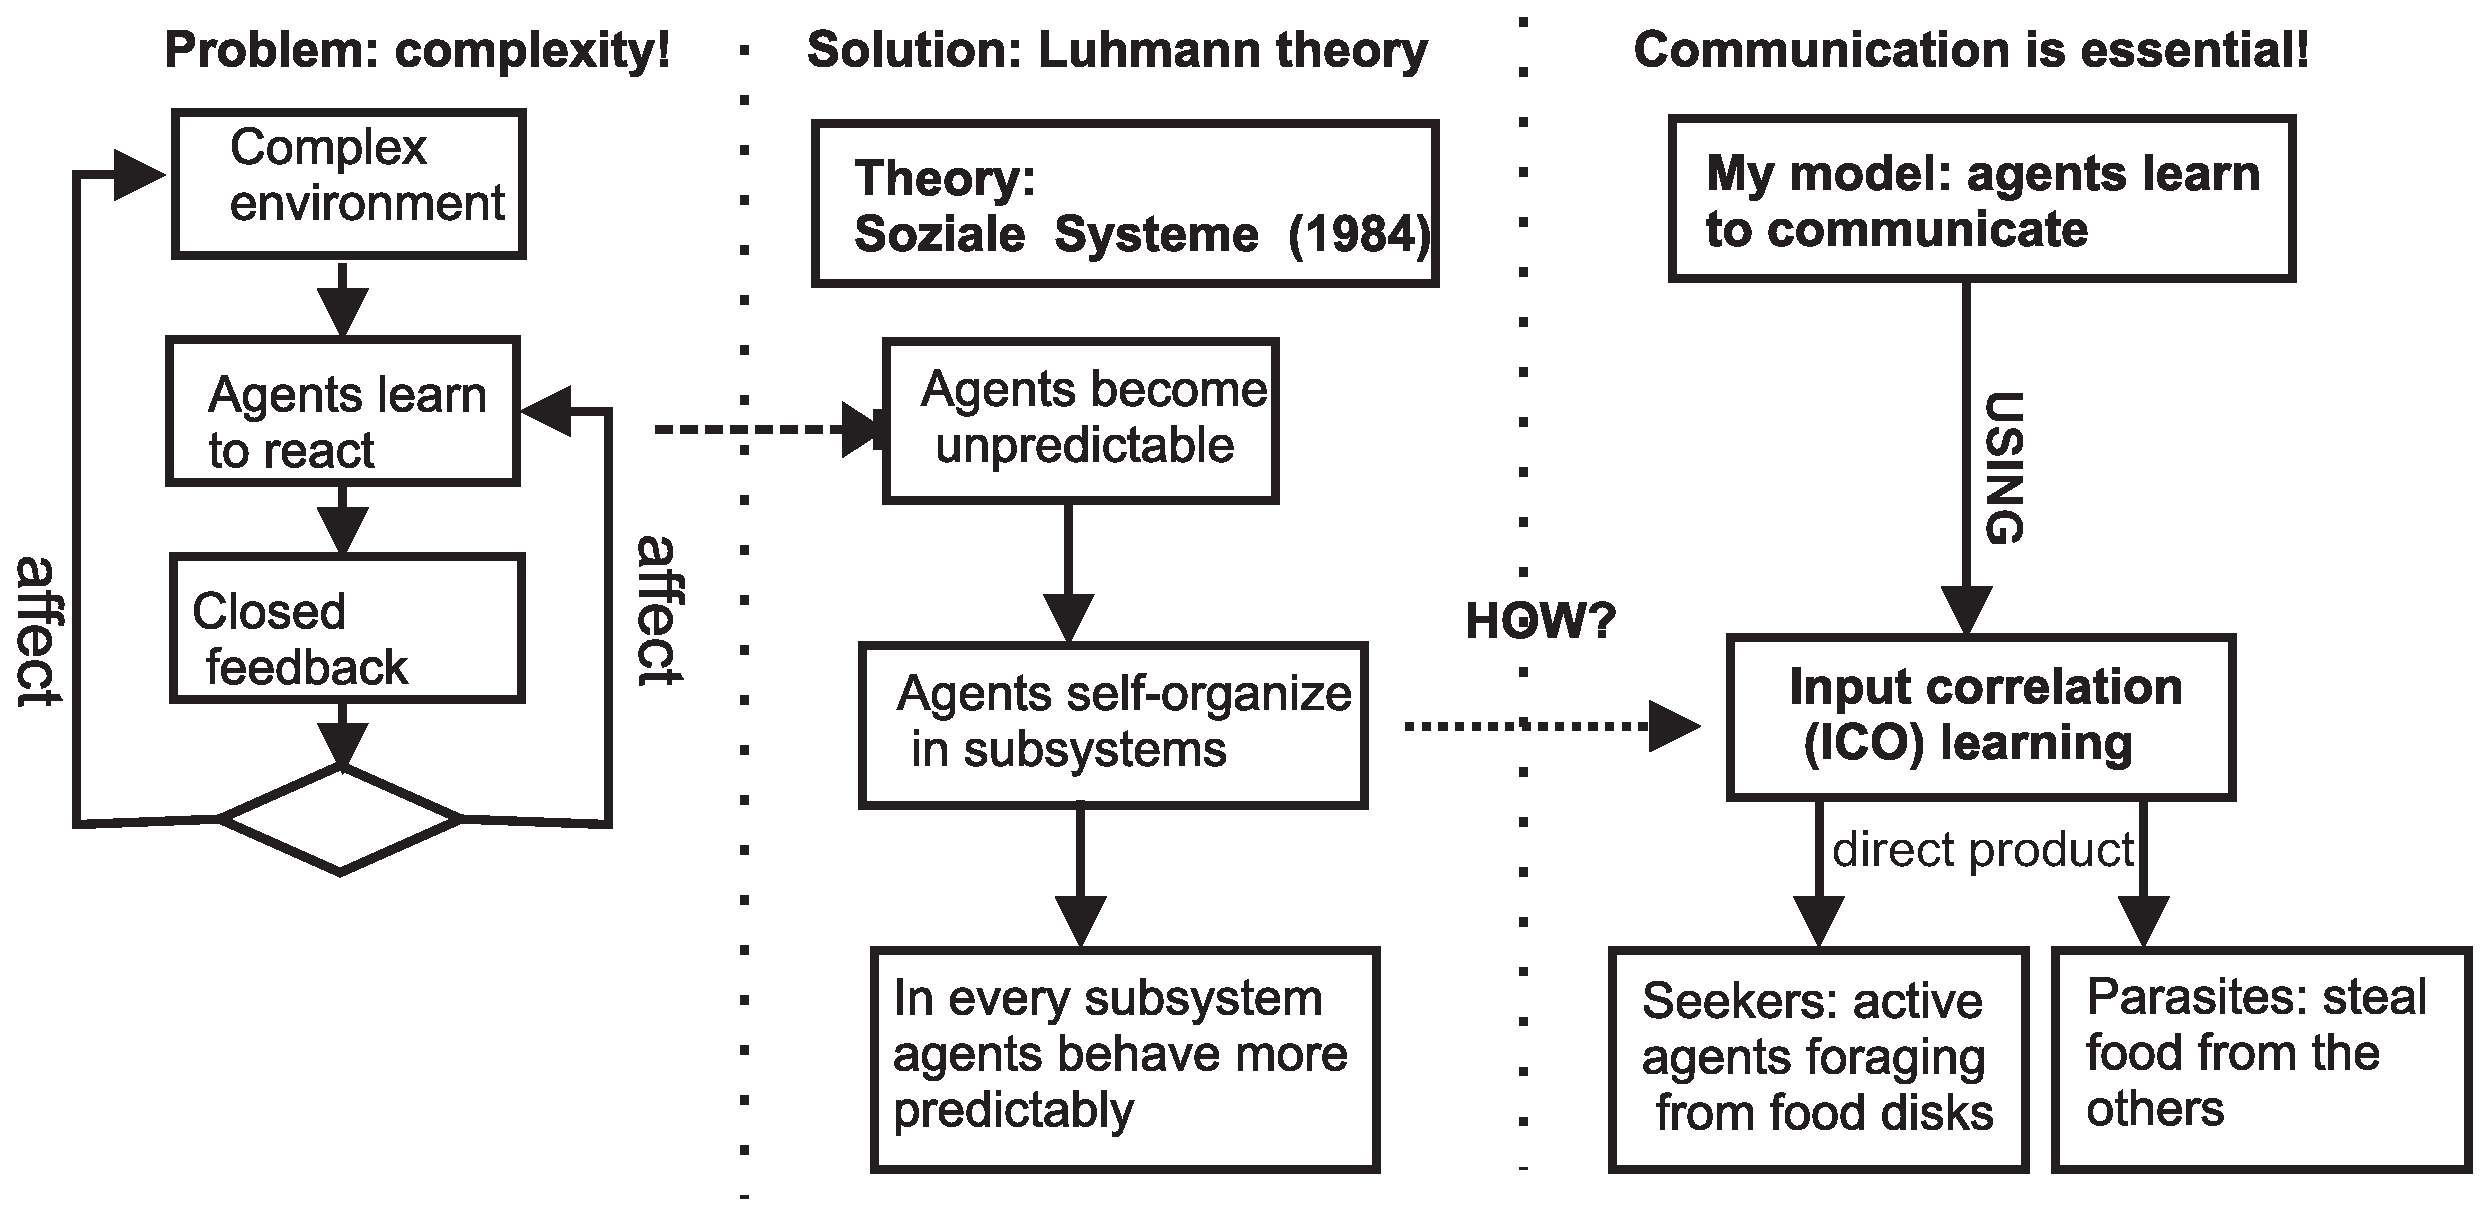
\includegraphics[width=1.0 \textwidth]{overview-1.eps}
\end{center}
\small{
\caption[Thesis research aim system]{Thesis objective at the system level \label{fig:overview-1}}}
\end{figure}

\begin{figure}[htbp]
\begin{center}
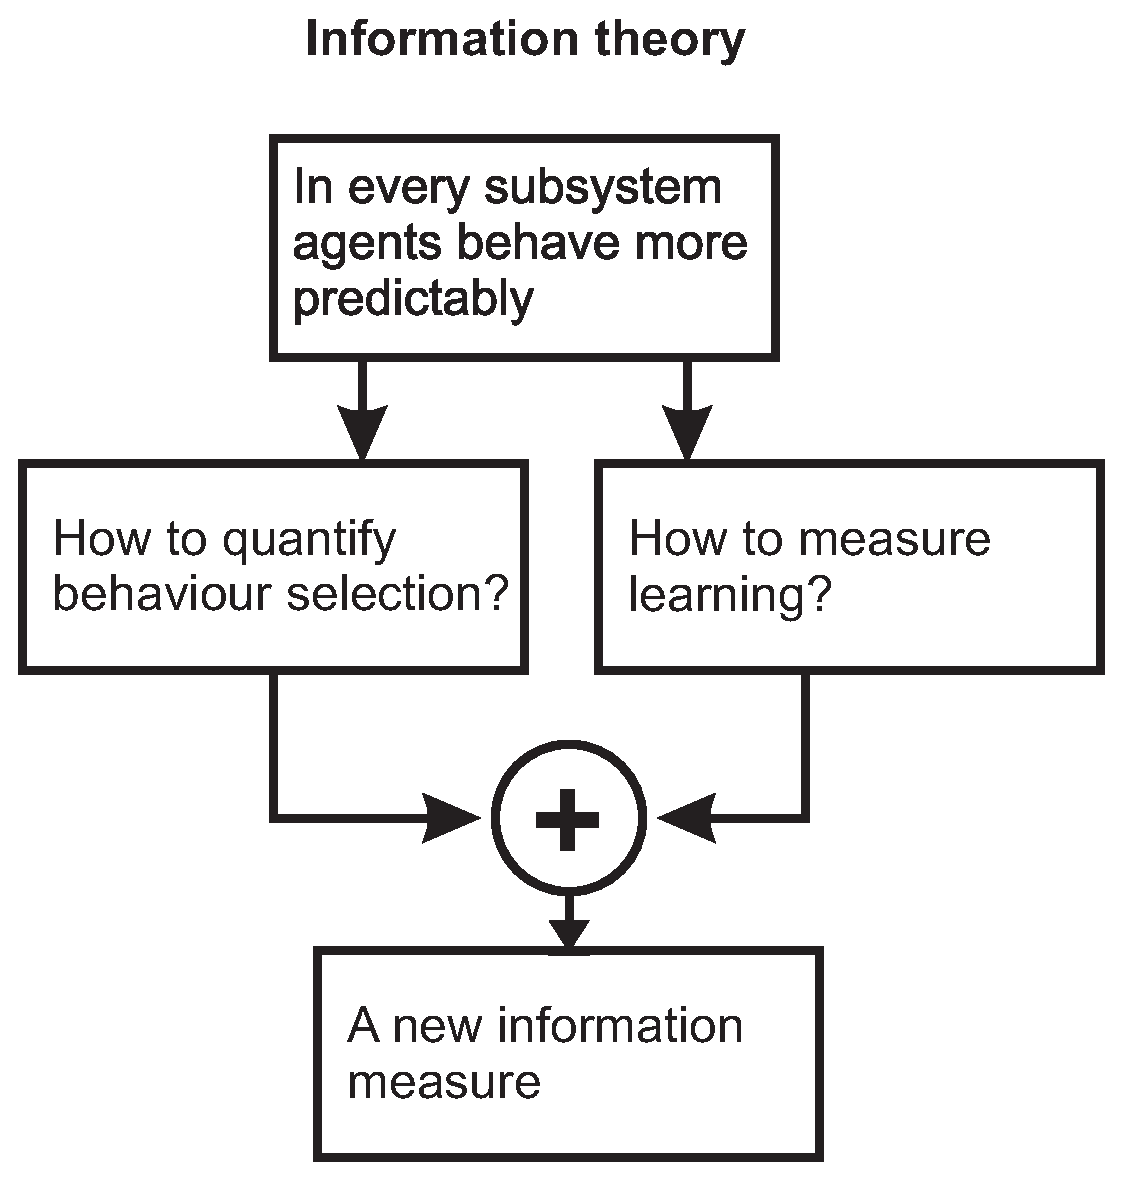
\includegraphics[width=0.5 \textwidth]{overview-2.eps}
\end{center}
\small{
\caption[Thesis research aim individual]{Thesis objective at the individual level \label{fig:overview-2}}}
\end{figure}
The aim of the thesis is to investigate the formation of sub-systems at a
system level as summarised in Figure \ref{fig:overview-1} and to
investigate the behaviour at an individual level as summarised in Figure \ref{fig:overview-2}.

The objectives of the thesis can be then summarised:
\begin{itemize}
\item implement a social system based on the Luhmann's hypothesis
\item verify the self-organising property (autopoiesis principle) of the system
\item measure the self-organising property of the system
\item quantify the self-organising property at the individual level with an
information theoretic approach
\item apply the same approach to different models
\end{itemize}

\section{Outline of thesis}
The thesis is divided into the following chapters:
\begin{itemize}
 \item this Chapter is a general introduction to this thesis
and a quick review of the existing literature.
 \item Chapter \ref{Chapter:Review} is a detailed review of literature closely related to this thesis.
 \item Chapter \ref{Chapter:Work} contains the main research and results
carried out by the author during his Ph.D.
 \item Chapter \ref{Conclusion} contains a summary of the results, a critical
comparison with the existing literature, a description of future work
and possible or existing industrial applications.
\end{itemize}

In Chapter \ref{Chapter:Work}, each Section was written to be a self-contained
module structured in the familiar order: Introduction, Methods, Results, and Discussion.
To avoid too much fragmentation a simple notation was used, for example in 
Chapter \ref{Chapter:Work}, Section \ref{Chapter7:Q learning application} 
is divided as follows:
\begin{itemize}
 \item Introduction: the application of information flow to Q-learning
 \item Methods: reinforcement learning
 \item Methods: Q-Learning algorithm
 \item Methods: Q-Learning connectionist
 \item Methods: The robot and the task
 \item Results: avoidance case
 \item Discussion
\end{itemize}
Each entry is then prefixed with the corresponding order.
All the sections are ordered in a logical manner, which does not correspond directly
to the chronological order of the research.
This happened for example with the Predictive Performance measure, which was
developed for a retinal robot and only after was applied to the data generated for
 the social system.
I have chosen a logical order so that the reader will be introduced gradually
to the topics.




\chapter{Background literature \label{Chapter:Review}}

\section{Introduction to the theory of Societies \label{Chapter1:SocialSystemTheory}}

This section contains an introduction to the theories about the generation of
human like societies and existing models in literature which replicate
artificial societies.

\section{A brief history of sociology}
Sociology is the study of society and aims to understand how social order is
possible.
In the last 350 years, sociologists have provided different explanations to the
generation of social order:
\begin{itemize}
 \item \citet{Thomas1651:Leviathan} attributed the generation to
a powerful state, the Leviathan
 \item \citet{Smith1776:WealthNations} attributed the generation
to an ``invisible hand''
 \item \citet{Durkheim1893} introduced the concept of norms
 \item \citet{Parsons1937:StructureSocialAim} extended the
Durkheim proposal by saying that norms are legitimated by values located in a
cultural system of a society
 \item \citet{Axelrod1984} suggested that the generation is
possible by rational choice of action with consideration for a long common future
(shadow)
\end{itemize}
A cardinal point in the theory of social order generation was introduced by
Parson as the \textit{the problem of double contingency}:
\begin{quote}
There are two crucial reference points for analysing interactions:
(1) That each actor is both acting agent and object of orientation both to
himself and to the others; and (2) that, as an acting agent orients to himself and
to others, in all primary modes of aspect. The actor is knower and object
of cognition, utiliser of instrumental means and himself a means, emotionally
attached to others and an object of attachment, evaluator and object of
evaluation, interpreter of symbols and himself a symbol. 
(International Encyclopedia of the Social Sciences,1968: 436)
\end{quote}

Following \citet{Talcott1968:SocioTheory,Luhmann95}
identified \textit{the problem of double contingency} as the main problem of
producing social order whilst expanding the idea with a new radical biological
principle called autopoiesis.

\subsection{Autopoiesis: from biology to social systems}
Luhmann based his social system theory on the concept of ``autopoiesis``,
originally formulated in biology by the two biologists \citet{Maturana1980}.
The biological concept of autopoiesis (from the Greek autos=self, poiein= to produce)
states that a living system recursively reproduces its elements through its own elements.
A living cell, for example, reproduces its own elements, like proteins or
and a plant grows its own leaves and roots.
The autopoietic system has 3 important properties and is described in Figure \ref{Fig:Autopoiesis:System}):
\begin{enumerate}
 \item operative closure: no operations can enter nor leave the system within its boundary
 \item interactional openness: the system has contact with its environment by means of disturbances
 \item structural coupling: environmental events can trigger internal processes but the internal
processes triggered are determined by the structures of the system
\end{enumerate}
The operative closure is symbolised by the partial feedback of the output to the 
input of the cell.
In essence autopoietic systems are at the same time open and closed systems;
open because they are influenced by their environment,
but also closed because environment does not directly
influence the structure and elementary processes of the systems.

The first and second property are also the basis of cognition:
\begin{quote}
Living systems are cognitive systems, and living as process is a process of cognition.
(Maturana and Varela 1980:13)
\end{quote}
The operations of an autopoietic system are defined as its cognitions: cognition is
a self-referential, autopoietic process.
This assumption is known as Radical Constructivism:
all ideas are constructs of the cognitive system and are a by-product of reality.
The most important contribution to the development of constructivism to neuro biological
 systems was pioneered by \citet{VanFoerster2003:Cybernetics}.
Every organism lives in a closed loop with its own environment and works only with neural activity.
The Figure \ref{Fig:Autopoiesis:Radical} shows how the cognitive system produces neural activity and
perceives neural activity: the environment is constructed as part of the feedback loop.
This self-reference property also exists at other layers, for instance in a call 
proteins create other proteins but the environment is coded as the protein production 
to maintain a membrane (made again by proteins).
This assumption is also important in the work of this thesis because artificial
agents, as well as human beings, construct their own reality. For instance a common behaviour
between animals is the natural reflex reaction to pain: when the skin is touching a
hot surface, the nervous system produces the idea of pain or heat.
The molecular property of the flame, triggered an action potential in the pain
receptor of the skin that then sent a reaction command in the motor cortex.
The physical event did not enter the cognitive system but only generated
a disturbance from the plateau state of the nervous system.

\begin{figure}[htbp]
\begin{center}
\includegraphics[width=0.8 \textwidth]{autopoiesis/neuralfeedback}
\end{center}
\small{
\caption[Radical constructivism example]{Radical constructivism example:
a burning flame is a physical system,
regulated by an oxygen reaction, when a finger touches it, a coupling is established
between the neural system and the flame.
The pain receptor produces neural activity, the brain generates a motor reaction, which then
 evokes an absence of sensory pain indicating that the reaction was good. 
The sensor produces again a different neural activity to encode the absence of pain.
\label{Fig:Autopoiesis:Radical}}}
\end{figure}

Later, in Section \ref{Section:ICOlearning} there is a clear explanation of the
implication of such an assumption.

The third property is the concept of self-organisation: the autopoietic system replicates
its elements by following a structure which is self-determined.
Thus we can  state that autopoiesis refers to the reproduction of the elements
and self-organisation refers to the determination of structures \citep{Luhmann2000}.

\begin{figure}[htbp]
\begin{center}
\includegraphics[width=0.8 \textwidth]{autopoiesis/maturanabiology}
\end{center}
\small{
\caption[Biological definition of autopoiesis]{The original definition given by Maturana and Varela:
An autopoietic machine is a machine organized (defined as a unity) as a network
of processes of production (transformation and destruction) of components which:
(a) through their interactions and transformations continuously regenerate and
realize the network of processes (relations) that produced them; and (b) constitute
 it (the machine) as a concrete unity in space in which they (the components)
exist by specifying the topological domain of its realization as such a network.
$[\dots]$ the space defined by an autopoietic system is self-contained and cannot be
described by using dimensions that define another space. When we refer to our
interactions with a concrete autopoietic system, however, we project this system
 on the space of our manipulations and make a description of this projection.
From \citet{Maturana1980} reproduced with permission of the publisher.
\label{Fig:Autopoiesis:System}}}
\end{figure}

Luhmann generalises the principle of autopoiesis to be a general form of system building
thus declaring that a system is autopoietic when it reproduces its own elements.
Figure \ref{Fig:Autopoiesis:General} describes the new hierarchy of autopoietic systems:
\begin{enumerate}
 \item level 1 contains the general definition
 \item level 2 contains living systems, psychic systems, neural systems and social systems
 \item level 3 contains societies, organisations and interactions
\end{enumerate}
Each system is described by the unit self-reproducible elements, in particular neural systems 
reproduces their own neural activity, living systems their own proteins and societies
 their own communications. 
In this thesis we are going to focus on the study of Societies \citep{Luhmann95}
which reproduce
themselves on the basis of communication and on the study of Neural Systems.
Moreover, Luhmann has also investigated the formation of organisations \citep{Luhmann2000} 
and social interactions \citep{Luhmann1993}.

\begin{figure}[htbp]
\begin{center}
\includegraphics[width=0.8 \textwidth]{autopoiesis/general}
\end{center}
\small{
\caption[General definition of autopoiesis]{Autopoiesis becomes a general
concept applied at different layers of
system formation. This thesis is focusing on studying the Social Systems.
\label{Fig:Autopoiesis:General}}}
\end{figure}

The next sections contains a descriptions of the neural systems that constitutes
the core of our artificial agents or robots.


\subsection{Neural systems \label{Introduction:NeuralSystem}}

The fundamental component of almost every living organism is its nervous system which
 is necessary for the the most vital activities like digestion, reproduction to the 
most complex ones like locomotion and cognition.
The most important assumption was made by \citet{VonFoerster85}, one of the founders of radical constructivism,
 who argued that the nervous systems is operationally closed: neural activity generates 
other neural activity and thus the environment is only a ''simulacra``.
The most basic type of a neural system is the reactive system, in control theory 
known also as a feedback system, which only reacts after a sensory event has occurred.
A feedback system can also be called a closed loop or self-referential system,
but I am going to use the most popular notation of closed loop system from now on.

\begin{figure}[htbp]
\begin{center}
\includegraphics[width=0.6 \textwidth]{neural/closedloop-1}
\end{center}
\small{
\caption[Closed loop reactive system]{
A simple closed loop system. 
Top: The transfer function $H_0$ transforms sensor signals
$X_0$ into motor signals $V$. The transfer function $P_0$ transforms the motor signals $V$
back into sensor signals $X_0$.
Bottom: the system can be simplified by dividing everything by $P_0$
\label{Fig:Neural:ControlReactive}}}
\end{figure}

The block diagram in Figure \ref{Fig:Neural:ControlReactive} represents a minimal system with feedback.
Each block contains the Laplace transform of the time domain function transfer:
\begin{itemize}
 \item $H_0(s)$ is the transfer function of the agent
 \item $P_0(s)$ is the transfer function of the environment
\end{itemize}
The transfer functions operates on neural signals which are the basic elements
 of the neurological system.
Because the systems is in closed loop form the following equations are valid:
\begin{eqnarray*}
  V(s)= H_0(s) \cdot X_0(s)\\
  X_0(s)=P_0(s) \cdot V(s) 
\end{eqnarray*}
Such a closed loop system can be stable or unstable and \citep{VonFoerster85} assumes,
like in traditional control theory, that it must operate in the stable state by 
using a negative feedback.
Stability is necessary in a linear system if the organism wants to reach a desired
 state after a finite time.
The main issue with this closed loop model is that the organism cannot distinguish
 itself from the environment because by dividing both the transfer functions by $P_0$,
the new transfer function $G(s)=H_0/P_0$ (see Figure \ref{Fig:Neural:ControlReactive}, bottom) 
does not distinguish any more from organism and environment due to the unity gain feedback. 
To avoid this issue, a disturbance $D$ must be defined as in Figure \ref{Fig:Neural:ReactiveDisturbance}.
The disturbance is anything which prevents the organism to keep its stable desired state 
and was also formulated by \citep{Ashby1956:IntroCybernetics} in its law of requisite variety which is going to
 be discussed in Section \ref{Chapter6:Information Flow}.

\begin{figure}[htbp]
\begin{center}
\includegraphics[width=0.8 \textwidth]{neural/closedloop-2}
\end{center}
\small{
\caption[Closed loop reactive system with disturbance]{
The closed loop system now contains a disturbance from the environment.
An example is the classical natural reaction to a burning sensation:
 the hand retracts when the pain receptor is activated by the contact
with the flame.
\label{Fig:Neural:ReactiveDisturbance}}}
\end{figure}

The disturbance this time cannot be eliminated by dividing the transfer functions by $P_0$.
A simple reactive system then can only react after a change it the desired state, 
a simple example is the motor reaction of our hand to a painful event like touching a 
flame. 
Another important point made by the radical constructivism theory is  that only actions which 
feed back to the organism's sensors can be observed by the organism. 
In the mentioned example then even a more complex motor reaction will only generate 
two possible state at the sensory input, one of pain and one of non pain.
Any other action which simply disappears in the environment cannot be
observed by the organism. Thus, there is no other chance for the organism as to
analyse its inputs as this is the only aspect that the organism is able to observe.
Even its own actions are only observable through its inputs.

A more advanced organism is one which has an anticipatory input signal $X_1$ as
 shown in Figure \ref{Fig:Neural:ProactiveDisturbance}:
when the agent is born only the inner loop $H_0,P_0$ is active but by using the 
association between $X_0$ and $X_1$ the agent can in the future avoid the 
painful signal by only using the anticipatory information $X_1$.
The reflex signal $X_0$ represents the initial behavioural
goal \citep{Verschure98summary} where $X_0=0$, while the predictive signal $X_1$
is provided naturally by the environment or the organism's sensor setup.

\begin{figure}[htbp]
\begin{center}
\includegraphics[width=0.8 \textwidth]{neural/closedloop-3}
\end{center}
\small{
\caption[Closed loop proactive system with disturbance]{
The inner feedback loop is established by the transfer functions $H_0$
and $P_0$. 
The outer feedback loop is established by the transfer functions $H_1$, $P_{01}$ 
and $P_1$. $D$ is the disturbance and $T$ delays the disturbance. 
The outer feedback loop observes the inner feedback loop and adjusts
so that the inner reflex loop is no longer needed.
\label{Fig:Neural:ProactiveDisturbance}}}
\end{figure}

The desired state, for example $X_0=0$ cannot be maintained all the time
as disturbances $D$ arrive at the loop occasionally. These disturbances enter
the inner loop delayed by time $T$. The undelayed disturbances enter the organism
via the sensor input $X_1$ which anticipates the input $X_0$ The signal at $X_1$
can now be used to observe the primary feedback loop ($X_0$,$P_0$) and determine 
what is the effect of on the primary feedback loop. This observation can be used to adjust
$H_1$ in a way that the inner feedback loop does not feel the disturbance any more.
This approach was succesfully implemented by \citet{PorrNecoISO2003} where a 
robot was using a camera system to learn the avoidance of obstacles.
The camera provided the visual anticipatory information required to predict the 
triggering of the touch avoidance sensor.
The robot used a learning statregy called $ISO$ which uses the correlation between
 vision and touch signals to learn the anticipatory reaction.
A more advanced form of $ISO$ called $ICO$ is used in this thesis as the main controller
 both for the software agent and the embodied robot.

The most interesting implication of this model when using multiple agents is the 
double contingency whereby each agent is disturbing the other as shown in Figure 
\ref{Fig:Neural:MutualDisturbance}.
Each agent is nested in multiple closed loops, because it receives the outputs of 
all the other agents in the environment via the disturbance summation with the 
environment itself.
Double contigency happens when all agents are learning continuously with, for example
ICO \citep{Porr2006ICO} or ISO \citep{PorrNecoISO2003} learning , from each other.
This learning loop was defined by Luhmann as the problem of double contigency:
an open ended interaction process where each agent try to predict the other.
A good metaphor is the game of chess where each player try to anticipate its opponent 
moves in the future: in a way the chess game is a sort of communicative process between
the two players which eventually comes to an end when the desired state (check mate) 
is achieved.
This dynamic process constitutes for Luhmann the necessary base for social generation.
It is possible that learning will never stabilise due to such multiple nested
 closed loops.

\begin{figure}[htbp]
\begin{center}
\includegraphics[width=0.8 \textwidth]{neural/closedloop-4}
\end{center}
\small{
\caption[Double contigency]{
Each organism output is summed to the motor feedback loop with the 
disturbance from the environment.
\label{Fig:Neural:MutualDisturbance}}}
\end{figure} 

Due to the complexity of such multiple interaction is not feasible to verify the 
property of stability and that is the reason why simulations were used in this 
thesis as the main tool.
In the social foraging task implemented in this thesis, learning stability was 
always achieved but it cannot be granted for every possible social task and 
must be verified case by case.
The ICO controller \citep{Porr2006ICO} was chosen to be the main block of each agent
 in my social model because they require simple computation, can be combined in parallel or series and
can be implemented in the analog domain or digital domain and have very good mathematical properties.
Another potential approach that was investigated prematurely was the use of 
model checking to predict the behaviour and properties of such a multi agent system and 
is discussed in the discussion section.
The next section contains a brief introduction to Braitenberg vehicles which 
are going to be used as the behavioural component of my artificial agents.

\subsection{Breitenberg vehicles \label{Intro:Braitenberg}}

A good controller is useless if it cannot be embodied in a physical robot.
The ICO and ISO controller were successfully implemented on a moving robot by
 adopting the approach developed by \citet{Braitenberg1986} who devised a simple
 yet effective method to implement avoidance and attraction behaviours on 
simple robots.
The most basic architecture is composed by a couple of sensory inputs, a couple of motors
and a matrix of connectivity which defines the behaviour of the robot.
The test case scenario is a vehicle moving on a planar surface which contains a light source
 be projected from above.
The vehicle has 2 light sensor which are able to measure the scalar gradient of 
the light source on the surface.
The motors are directly connected to the sensors via positive or negative proportional 
controllers.
Figure \ref{Fig:Braitenberg:Example1} shows that an avoidance behaviour can be implemented
 by using positive feedback connections:

\begin{itemize}
 \item a vehicle with symmetric connections from sensors to motors, dislikes the source 
of light by constantly avoiding it.
 \item a vehicle with crossed connections from sensors to motors, dislikes the source of light
but constantly turns toward it at maximum speed, as if it wanted to destroy it.
\end{itemize}

\begin{figure}[htbp]
\begin{center}
\includegraphics[width=0.8 \textwidth]{vehicles/Braitenberg-1}
\end{center}
\small{
\caption[Braitenberg vehicles positive feedback]{
An example of a coward and aggressive vehicle with only positive feedback connections.
\label{Fig:Braitenberg:Example1}}}
\end{figure}

Figure \ref{Fig:Braitenberg:Example2} shows that an attraction behaviour can be implemented
 by using negative feedback connections:
\begin{itemize}
 \item a vehicle with symmetric connections from sensors to motors, likes the source 
of light by carefully approaching it and reaching ideally zero velocity in proximity.
 \item a vehicle with crossed connections from sensors to motors, likes the source of light
but constantly search for other alternatives 
\end{itemize}

\begin{figure}[htbp]
\begin{center}
\includegraphics[width=0.8 \textwidth]{vehicles/Braitenberg-2}
\end{center}
\small{
\caption[Braitenberg vehicles negative feedback]{
An example of a lover and explorer vehicle with only negative feedback connections.
\label{Fig:Braitenberg:Example2}}}
\end{figure}

The behaviour of such vehicles can be enriched by including more sensors and so
 mixing positive and negative connections or by using non monotonic relationships
 between sensors and motors.
The agents that I used in the software simulations and robot implementations, 
are based on the Braitenberg framework but enriched with the power of ICO learning 
\subsection{Communication}
For Luhmann, the most important feature of a social system is that communication
is the basic form of the autopoietic reproduction of social systems.
Social systems consist of communicative processes (see Figure
\ref{Fig:Autopoiesis:Communication}), not human beings.

\begin{figure}[htbp]
\begin{center}
\includegraphics[width=0.8 \textwidth]{autopoiesis/elements}
\end{center}
\small{
\caption[Communication is the basis for society]{Living systems are based
on cellular mechanisms of reproduction and
their elements are proteins and molecules. Social systems are based on communication
processes which reproduces themselves. Psychic systems are based on self-reproducing
thoughts. Each system is structurally coupled with each other.
The structural coupling between psychic systems and communications is established
through Language. Language allows the ''synchronization`` between the two systems
but communication is also possible without it.
\label{Fig:Autopoiesis:Communication}}}
\end{figure}

Human beings are individuals in a society only when they communicate and
thus the limit of society is defined by the limit of communication.
Communication has been defined by Luhmann as a unity of 3 selective
and independent processes:
\begin{itemize}
 \item utterance: how do we utter it?
 \item understanding: how do we separate utterance from information?
 \item information: what was the utterance about?
\end{itemize}
Communication is an \textbf{emergent property} of the interaction between two psychic systems
as the three selections do not belong to each individual independently.
Each step is considered by Luhmann as a selection process from a set of possibilities,
in accordance with the definition of information of Shannon and Weaver \citep{Shannon1948}.
To explain the communication process Figure \ref{Fig:Autopoiesis:CommExample}
contains an example of a communication session between Ego and Alter.
The psychic system embodied in Ego has the intention or desired state of being alone
 because he/she is tired.
The first step for Ego is to select the appropriate utterance which in this case 
is the English sentence ''go away``.
At this point Alter receives the utterance and needs to understand it by extracting the 
information from it.
Alter then can decide to leave or to continue the conversation. Assuming that in the first
case, he leaves Ego alone and emits an utterance like ''Oky``, Ego will understand that 
its initial utterance ''go away`` was successful.
On the contrary if Alter persist and does not leave Ego alone, Ego will try
 indefinitely to produce other utterances until Alter leaves.
 
In Figure \ref{Fig:Autopoiesis:CommExample} Ego can also accept or reject the
meaning of the communication which implies a dynamic selection mechanism for
the continuation or interruption of the communication process.

\begin{figure}[htbp]
\begin{center}
\includegraphics[width=0.8 \textwidth]{autopoiesis/dialogexample}
\end{center}
\small{
\caption[Communication between alter and ego]{
Ego is a psychic system with a current goal or desired state.
When Ego is in contact with Alter in a contingent situation. he selects the utterance 
''go away`` to be communicated to Alter. Alter then needs to extract the 
meaning from such an utterance and infers that Ego wants to be alone. 
Then Alter can decide to continue in the conversation or quit it by just leaving
 Ego alone.
The acceptance or rejection of the understanding is an option in the communication.
\label{Fig:Autopoiesis:CommExample}}}
\end{figure}

The Luhmann interpretation of communication is therefore far more advanced
than the simple channel communication theory where the purpose is to transfer
meaning with minimal errors.
In this sense there is similarity with the work of \citep{Berger1975:URT} 
who developed an axiomatic theory to explain people's attempts to “make sense” of interpersonal
situations by reducing uncertainty through seeking information.
Additionally the concept of reducing uncertainty
during the understanding process being a motivation to continue a communication 
is not mentioned in the original work.
There is also another interesting implication of using Luhmann's communication 
which fits recent theories of the mind.
The use of expectations is tightly linked with the idea of estimating each other's
state of mind as described with greater detail in Section \ref{TheoryOfMind} and \ref{Conclusion:Language}.
So in summary, communications can reproduce themselves but what communications
are produced is related to the concept of expectation.
In the next section I am going to introduce the most relevant simulation model 
which captures the social ordered generation by using such a model of communication 
based on expectations.

\section{Social order generation by double contingency \label{Introduction:SocialOrderModel}}

The starting point for implementing a simulation which uses Luhmann's communication approach, 
was developed by \citet{SocialOrderScalability} which implemented the situation of
double contingency as the origin of social order.
The results produced by this approach were very promising


\subsection{Methods}
He started from a dyadic social interaction and then expanded it to a multi agent interaction.
Social order appears in the dyadic social interaction and also in the multi agent situation,
but only in certain conditions that we are going to explain.

The double contingency problem exists when a dyad composed of 2 entities (ego and alter) meet each other:
each actor has a double role of knower and object of cognition.

Parsons solved the problem of contingency by asserting that a common shared symbol system
is a pre-condition for the formation of a social order.
Therefore the dyad must share a culture derived from a history of previous relationships.

Luhmann solves the problem of double contingency by using a self-organisation process which
develops in time based on mutual expectations.
The only hypothesis he made was that alter and ego (the actors in the dyad) have a
necessity of predicting ``expectation-certainty'', which means Alter and Ego want to know what
is going on in this interaction.
Every entity expects that the other entity has expectations about its next activity.

The desire -or goal- of every agent during the interaction is to reduce the entropy -uncertainty- of the
Alter's actions given Ego's actions.

To give a simple example, when I say ``Hello'' to a friend, I expect to receive a ``Hello`` followed by
a form of embrace, typically a handshake possibly followed by a conversation. My friend will expect the same.
This is useful as we don't have to try out all our vocabulary every time to get somebody's attention!
Figure \ref{Fig:Dittrich:Model} explains the model with a simple example where
Ego says ''Good morning`` and alter replies with ''Good morning``, then Ego
asks ''How are you?'' but Alter ask a question about time.
This somehow puzzles Ego -delusion- because he wasn't expecting a question after
his question.
\begin{figure}[htbp]
\begin{center}
\includegraphics[width=0.8 \textwidth]{autopoiesis/expectations}
\end{center}
\small{
\caption[Expectations and communication structures]{
Upper block: an example of mutual expectation in a conversation.
Lower block: the simulation model with the Expectation-Expectation memory
and the Expectation-Certainty model.
\label{Fig:Dittrich:Model}}}
\end{figure}

So the model proposed by Dittrich begins with a simple dyad of 2 actors:
\begin{itemize}
 \item Ego initializes the interaction by choosing a message from a set of N possible ones
 \item Alter receives the message and replies with another one from the set of N
 \item the conversation continues from Ego and so on
\end{itemize}
The activity of an actor is to decide which message has to be sent given a received message.
This kind of action is a reduced model of Luhmann's communication because there 
is no distinction between information, transmission and understanding.
Ego chooses the message and sends it (information $+$ transmission) and
replies to the message without understanding it.
Also, agents do not show a motivated behaviour towards others, according
to goals and a shared symbolic system, as proposed in the Parson's model.

Each agent is motivated by 2 functions:
\begin{itemize}
 \item Expectation-Expectation \textbf{EE}: an agent wants to meet the
expectations of the other agent. It does so by keeping a memory of what actions
were chosen in response to other agents.
 \item Expectation-Certainty \textbf{EC}:  the reaction of the other agent
following its own activity should be as predictable as possible.
 \item Activity Value: a linear combination of $(1 - \alpha)EE + \alpha EC$.
 \item Activity Probability: a parameterised version of the activity
value $\gamma$ that can go from deterministic $\gamma \rightarrow \infty$
to probabilistic $\gamma \rightarrow 0$ .
\end{itemize}

Each agent chooses the activity which maximises the activity probability according
 to the parameter $\gamma$.
The parameter $\alpha$ accounts in a way the ''selfishness`` of the agent because
when $\alpha=1$ the agent will choose the action that will produce the most likely
reaction from Alter whereas when $\alpha=0$ the agent will choose the action
that Alter will expect more.

The problem is then to measure Social Order and see if the dyadic condition is
able to produce high values of social order. There are 2 different points
of view: a system view and an individual view.

At the individual level we can re-use the EC function to compute how certain
an agent is when it selects a message.
The average certainty $O_AV$ has a high value when certainty is high and thus
indicates high social order.

At the system level we can measure:
\begin{itemize}
 \item the average number of different activities $N_D$ selected during the
time interval: the lower the number the higher the order. An observer will
deduce that high social order is achieved if agents always select the same
activities out of a vast selection set.
 \item predictability of an activity $O_p$ or social integration: it measures
how predictable an activity of a randomly drawn agent Ego is, given the
activity presented on the sign by another randomly drawn agent Alter.
\end{itemize}

We can interpret the $O_p$ value as an index of the pattern formation in
the behaviour of action selection. The actors formed a closed system of
interaction because they are required to develop mutually predictive trust,
this closure indicates a first order separation degree between a system and its environment.

\subsection{Results}
For the dyadic case social order as measured either by $N_D$ and $O_AV$ emerges
for any parameter setting in $\alpha,\gamma, N$ with stable activity patterns
following robust to small disturbances.
Measuring social integration for the dyadic case is trivial because there are
only 2 agents who interacted with each other and thus it will be $O_p=1$.

The big challenge is then to scale up the dyadic case to the multi agent case.
If we have a population of few $M$ agents and we choose a random selection strategy
to pair interactions,
social order is high in terms of $O_P$ because is possible to predict each agent's 
reaction with a high degree of accuracy.
However at the individual level $O_AV$ is low because each agent is using the
 same memory to predict interactions with different agents.
As a consequence increasing $M$ decreases the $O_P$ system order.

Dittritch discovered that there are 2 changes required to produce high social
order with an increasing number of agents:
\begin{itemize}
 \item agents must calculate Expectation-Expectation from observation of the interaction of other agents
 \item agents must use only Expectation-Expectation for activity selection ($\alpha=0$)
\end{itemize}

At the individual level agents are cognitive entities able to perceive, memorise,
generalise and to make predictions.
For society to emerge they must be able to observe the interactions between others.

\subsection{Discussion}
The results of such a model were quite promising but there are also some weaknesses:
\begin{itemize}
 \item the system operates exclusively on a symbolic communicative system
 \item the system does not distinguish between actions which manipulate the environment 
and communications 
 \item the system is discrete and cannot operate in the analog domain
\end{itemize}

The mentioned issues were the main drives for the model described in this thesis because 
if such a social system needs to be implemented in the real world, the agents 
or robots needs to have a separate layer, one for the actions in the environment and one
 for the communicative events which are essentially symbolics.
Another desired property is the use of analogic based controllers which can 
then be implemented in very fast reactive electronic controllers or also 
digitized and implemented on a micro controller.
In the next section, I am going to describe the framework used to achieve such targets.





\section{Agent Based Modelling \label{Chapter3:ABMcomplex}}

This Section contains a summary of current modelling strategies for the simulation
of software agents which interact with each other like animal groups or human societies.

\subsection{SWARM and ABM}
The simulations of artificial agents in this Thesis were done by using an ABM approach.
In literature there is, unfortunately, a conflict in notations as well as several debates
in the differences between MAS\nomenclature{MAS}{Multi Agent System}, ABM (agent based models) and
SWARM\nomenclature{SWARM}{Collective behaviour of animals} intelligence.
The expression SWARM intelligence \citep{SwarmIntelligence} was introduced by
Gerardo Beni and Jing Wang in 1989, in the context of cellular robotic systems.
SWARM refers to a form of collective behaviour exhibited by groups of
 homogeneous animals: flocking is the swarm behaviour of birds,
herding is the swarm behaviour in quadrupeds, schooling is the swarm behaviour
in fish.
The definition given by the leader in this field Dr.Marco Dorigo follows:
\begin{quote}
Swarm intelligence is the discipline that deals with natural and artificial systems
composed of many individuals that coordinate using decentralized control and self-organization.
In particular, the discipline focuses on the collective behaviours that result from
the local interactions of the individuals with each other and with their environment.
Examples of systems studied by swarm intelligence are: colonies of ants and termites,
schools of fish, flocks of birds and herds of land animals. Some human artefacts also
fall into the domain of swarm intelligence, notably some multi-robot systems,
and also certain computer programs that are written to tackle optimization and
data analysis problems \citep{Dorigo:2007}.
\end{quote}
Swarm intelligence has been used to model the clustering behaviour of
ants, the nest building behaviour of wasps and termites,
flocking and schooling in birds and fish.
Particle swarm optimisation \citep{JamesShi2001:PSOgeneral}
is a population based stochastic optimisation technique for the solution of
continuous optimisation problems and therefore is used more in the realm of
functional mathematics.


The simulations used in this Thesis cannot be considered as Swarm simulations because
the agents are active learners and share some features with human like societies
rather than animal societies like ants.
Therefore the author will use the term ABM for referring to the actual implementation.
Nevertheless, there are some human behaviours like panic behaviour that can be
described as herding behaviour and thus can be still classified as Swarm behaviour
\citep{Bonomi2009:PedestrianDynamic,Georgoudas2006:PedestrianEvacuation,Kirchner2002:CASim,
Varas2007:CAevacuation,Zong2010:MultiObjAnt}.
The choice of the ABM term for my simulations in this Thesis was made for clarity
and to classify the work in this fast growing sector.

Research in ABM involves the investigation of autonomous, rational and flexible
behaviour for entities such as software programs or robots, and their interaction and
coordination in several areas including: robotics \citep{Kitano1997},
information retrieval and management \citep{IntroMultiAgent1,IntroMultiAgent2}
 and simulation \citep{GilbertConte1995:AIsocieties}. When designing agent systems, it is
impossible to anticipate all the potential situations an agent may encounter and to optimally
specify an agent behaviour in advance. Agents therefore have to learn from,
and adapt to, their environment, especially in a multi-agent setting.
This is especially true for multi-agent systems where in many cases global behaviour
emerges rather than being pre-defined.

ABM can be seen as the natural extension of the Ising model \citep{Ernst1925:Model} or
Cellular Automata-like models \citep{Wolfram1994:CellAutomata} which have been very successful
in the past decades at describing various physical phenomena like Ferromagnetic materials.

One important characteristic of ABMs, which distinguishes them from Cellular Automata,
is the potential asynchrony of the interactions among, and between, agents and
their environments. In ABM agents typically do not simultaneously perform actions at
constant time-steps, as in CAs or boolean networks. Rather, their actions follow
discrete-event cues or a sequential schedule of interactions. The discrete-event
setup allows for the cohabitation of agents with different environmental experiences.
Also ABMs are not necessarily grid-based like the Conway's game of life \citep{Gardner1970:GameLife} 
and can also simulate analogic agent controllers.
In particular, the richness of detail one can take into account in ABM makes
this methodology very appealing for the simulation of biological, social and
economic systems; where the behaviour and the heterogeneity of the interacting
components are not safely reducible to some reduced models or differential equations.

In essence the two reasons for the choice of ABM in this thesis are:
\begin{itemize}
 \item simulation in real time of parallel analog or discrete processes
 \item flexibility in the implementation of hardware based robots
\end{itemize}
To make a concrete case in Appendix \ref{Appendix:RobotSystem}, the software agent 
was implemented on a robotic kit called Lego and on a small robot called Pololu 3PI 
and in Appendix \ref{Appendix:simulation} there are some code examples taken from
 the Enki simulator which is able to describe the mechanical and electronical properties
 of a real Alice or Keplera robot including for example the motor noise and the jerkiness 
of the stepper motor.



\subsection{Single agent VS multi agent learning}
There are two main approaches to ABM systems and learning:
\begin{itemize}
 \item ``single agent learning``: existing machine learning algorithms are applied
directly to single agents in a MAS setting. Consequently, multi-agent learning is only
seen as an emergent property.
\item ''multi agent learning``: agents need to cooperate and communicate in order
to learn effectively.
\end{itemize}

Single agent learning \citep{StoneVeloso98:RoboCup,Porr2006ICO,Porr2003b} 
focuses on how one agent improves
its individual skills, regardless of the domain in which it is situated.
As discussed before, thanks to the closed loop property of such controllers the 
organism can still learn from the others by means of their motor actions which 
feedback into each others' inputs: each agent perceives the others as part of the environment feedback loop.
Previous research studies have shown how is possible to create  coordinated group behaviour 
with pure single-agent learning \citep{Sugawara98learningto}.
This is also the case, as we are going to see, for the model that is used in my research which
contains also a communication layer through which agents learn to cooperate in a foraging task.
Thus in my model each agent learns with a predictive controller \citep{Porr2006ICO}.
We investigate the influence of communication in the Section \ref{Chapter4:Social adaptation} 
where the property of double contingency is used succesfully to reproduce social order
 in artificial societies.





\section{Information theory for closed loop controllers \label{Introduction:InfoTheoryClosedLoop}}

This section contains the essential background for the application of information
theory to closed loop controllers.
It will be used extensively for the computation of information measures in the 
following sections.

\subsection{Introduction: closed loop controllers}
In control theory there are two main approaches: open loop control and closed
loop control. Open loop control is possible only when the law or transfer of the
 process I want to control is known. Natural systems are very hard to control
using the open loop approach because they are dynamic non-linear processes and
their parameters are subjected to noise. Closed loop control does not require
the full knowledge of the process and is based on the principle of action and reaction.
Adaptive controllers change their parameters according to the observed parameters of
the process to control: most biological organisms use the control loop approach.
The daily process of maintaining our body temperature is an example of such a system \citep{HumanBody}.
Until today cybernetics has provided a lot of adaptive controllers for the closed loop:
PID\nomenclature{PID}{Proportional Integration Derivative control} controllers
(see Figure \ref{Figure:maxcorr:PID}) and the Kalmann filter to mention the most important.
\begin{figure}[ht]
  \begin{center}
    \includegraphics[width=0.6 \textwidth]{maxcorr/InfoAgentTheory-2.eps}
    \caption[Classical PID controller]{
	     A classical PID controller described only by the proportional gain.
	      \label{Figure:maxcorr:PID}}
  \end{center}
\end{figure}
Artificial intelligence (AI) branched from cybernetics and used what was available
from the previous approaches, but it realised that designing artificial agents
for the real world using the previous
approaches was not possible: agents must be bio-inspired to live in our world.
Hebbian learning, neural networks, Q-learning, fuzzy logic and many others are
nowadays used in many artificial agent systems. However using these adaptive
controllers raises a big concern: how can I assess the performance of the agents?
The question is not as trivial as it seems: the agent adapts to the environment,
thus in general a more complex environment produce a more complex
behaviour \citep{NolfiInteraction}. 
But agents essentially perform input control to keep their desired state.
The only solution to that problem is to develop input based measures and not 
output based measures as I will demonstrate in Section \ref{Chapter5:Max Corr Input}.
Input contains the output of the agent through the environment,
therefore if the agent is learning, it means it is changing the inputs to achieve
a desired state (for example avoiding a painful signal).
This approach was introduced by Gibson \citep{Gibson1955:learning} who rejected
cognitivism and behaviourism for a more direct realism. 
He argued that organisms perform only input control, one of his most radical
 approach was the concept of ``affordances'' whereby the objects of our environment
 tell implicitly how they want to be operated.
Although there are some cases where organisms perform open loop forward control,
 the general principles described by Gibson are valid.
the general model is described in Figure \ref{Figure:maxcorr:Gibson}.

\begin{figure}[ht]
  \begin{center}
    \includegraphics[width=0.6 \textwidth]{maxcorr/InfoAgentTheory-4.eps}
    \caption[Gibson cybernetic approach]{
	     Gibson model of perception: the agent can only act and sense
	     on a sub-dynamic of the environment.
	     \label{Figure:maxcorr:Gibson}}
  \end{center}
\end{figure}

The theory of Shannon's information cannot be applied directly in closed loop
 systems because the information flow in an organism is asymmetric
(see Figure \ref{Figure:maxcorr:asymmetry}).
In the agent perspective the action is sensed via a representation of the
controlled process.

\begin{figure}[ht]
  \begin{center}
    \includegraphics[width=0.6 \textwidth]{maxcorr/InfoAgentTheory-3.eps}
    \caption[Information asymmetry in the organism]{
	     The problem of information asymmetry in the closed loop control case.
	      \label{Figure:maxcorr:asymmetry}}
  \end{center}
\end{figure}

In fact the traditional notion of Shannon entropy was extended to closed loop
systems by considering the sensory-motor loop as a communication channel which 
extends in time to propagate information from and to the environment.
For example \citet{Touchette2004} revisited the idea of a controller as
 an actuation channel that transforms input states to desired output states.
He also gives necessary and sufficient conditions for a system to be perfectly
 controllable and perfectly observable in terms of information and entropy.
His model is a Bayesian network composed by a sensor channel $S$,
an actuator channel $A$, the initial state of the system $X$ and the final
state of the system $X'$. The model as described in Fig. \ref{fig:tishby1} both
represented in Shannon's terms by their probability distribution matrix $p(a|s)$,
where $s$ is the input random variable of the channel and $a$ the output random
variable of the channel.
The controller is modelled as a random variable $C$ that takes an initial state
 $X$ of the system to a final target state $X'$. A closed loop controller chooses
a regulation $a_i \in A$ based on the state of the system $x_i \in X$, whereas an open loop
 controller chooses a regulation $a_i \in A$ that is independent of the sate of the system $x_i \in X$.
Open loop control is thus different from a closed loop control in terms of
mutual information $I(X,C)$ as described in Eq. \ref{infotheory:eq:control}: 
\begin{eqnarray}
open \; loop &:& I(X;C)=0\\
closed \; loop&:& I(X;C)>0
\label{infotheory:eq:control}
\end{eqnarray}

\begin{figure}[!htbp]
\begin{center}
\includegraphics[width=0.8 \textwidth]{ashby/figure-2}
\caption[Bayes formulation in traditional control]{
Bayesian formulation of open and closed loop.
A) Full control model.
B) Reduced open loop model.
C) Reduced closed loop model.
D) Single actuation channel model.
The only way to distinguish open loop from closed loop is by means of Eq. \ref{infotheory:eq:control}.
\label{fig:tishby1}
}
\end{center}

\end{figure}

The controller can be extended for the predictive case introduced in section \ref{Introduction:NeuralSystem},
by adding an additional variable $Y$ which is the predictor of $X$ as in Fig. \ref{fig:tishby2}:
$Y$ conveys information about $X$ and is used by the controller to infer the 
temporal relation between the predictor $Y$ and the reflex $X$.
This Bayesian model is investigated more in depth in section \ref{Conclusion:PredictiveBayes}.
\begin{figure}[!htbp]
\begin{center}
 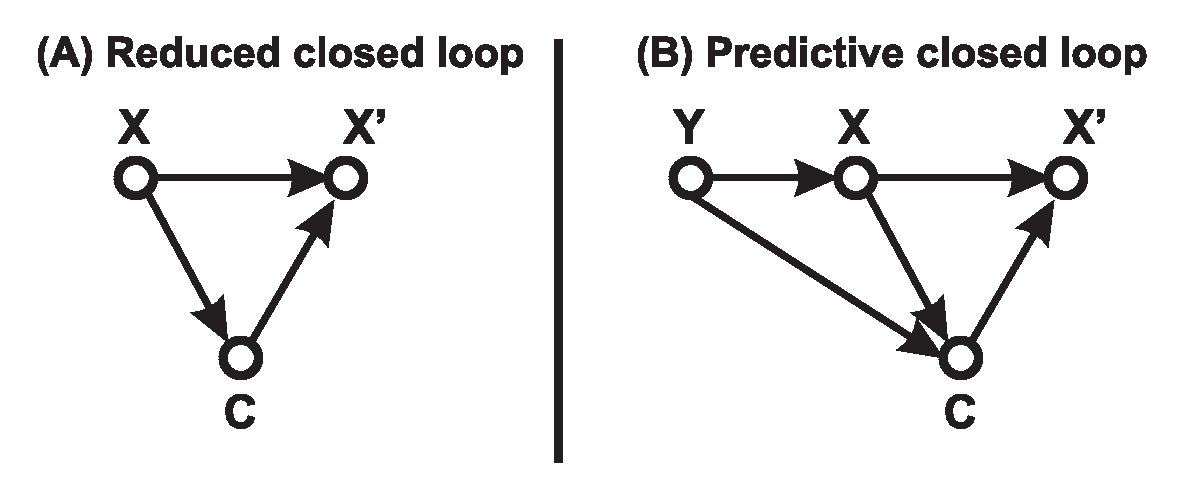
\includegraphics[width=0.8 \textwidth]{ashby/figure-4}
\caption[Bayes formulation in predictive control]{
Extended Bayesian formulation.
\textbf{A)} open loop case with sensor collapsed into controller $S=C$.
\textbf{B)} closed predictive loop with $Y$ predictive signal on $X$.
\label{fig:tishby2}}
\end{center}
\end{figure}

Other important tools were provided by \citet{Tishby1999:InfoBottle} with the 
the information bottleneck method which considers the ability of learning 
in predictive controllers related to the compression achieved when two or more
signals are mutually dependent.

The first practical application of information measures to closed loop controllers
was introduced by \citet{organizationInfo} who used the Tishby's framework
to implement an information based controller as described in Fig. \ref{fig:conclusion:polani}.
The approach used is similar to the one described in Fig. \ref{Figure:maxcorr:asymmetry} 
but with an optimization value provided by the information flow: the controller's
transfer function is a model of the environment and the goal of the controller
consists in maximizing the information flow from the motor output to the sensory input.
With this very general approach the controller is able to achieve meaningful states
without even defining a task objective.
The disadvantage of the approach is that the controller needs to have a good model
of the environment and needs to be able to do simulations and choose the best
path to maximize the information flow.


\begin{figure}[htbp]
\begin{center}
\includegraphics[scale=0.3]{figures/conclusion/polani2008.eps}
\end{center}
\vspace*{4pt}
\caption[Empowerment from Polani]{
The empowerment is defined as the maximum information flow
from the action $A_{t}$ to the sensors $S_{t+1}$ via the environment $R_{t}$.
The source of uncorrelated randomness $Z_{t}$ is useful to assess the controllability
when the organism is removed from the control law.
\label{fig:conclusion:polani}}
\end{figure}

A more general approach was introduced by \citet{LungarellaInformation} which
used several information based metrics to follow the learning curve of the robot
in a visual foveation task: the robot reduces the entropy around the centre of focus.
\citet{LungarellaInformation} describes a closed loop system as a system which
decreases the entropy, increases the information structure (statistical regularity),
decreases the complexity.

A similar approach was used by \citet{Ay2008:PredInformation} to modify the proportional
coefficient in the controller's function to allow an optimal exploration strategy
of an environment with obstacles: the mutual information between paste and future
is used to tune the gain $c$ so that the maximum of the predictive information defines the best exploratory
behaviour.

The main contribution earlier than Tishby to the cybernetic theory of controllers
was produced by Ashby in 1956 and it will be used heavily in this thesis.
Therefore the next section contains an overview of his framework.

\subsection{Regulation and entropy \label{Appendix:Ashby}}

\citet{Ashby1956:IntroCybernetics} defined clearly that the
 essential feature of a good regulator is to block the flow of variety from
disturbances to essential variables. Ashby uses variety precisely as the number
 of different states a variable can be and is equivalent to Shannon's entropy.
Thus variety and entropy can be used alternatively.
I use the same notation by Ashby so that it will be more clear how those concepts
can be applied successfully to predictive learning:
\begin{itemize}
 \item D is the domain of disturbances from the environment like a threat for an organism.
 \item E is the domain of the essential variable, can be partitioned in
$E= \eta \cup \overline{\eta}$, where $\eta$ is a partition of desired states
 or goals of the organism and its complementary partition $\overline{\eta}$
 represents the non-desired states.
 \item R is the domain of available regulations that the organism can perform
 \item T is the domain of the possible states of the environment.
 \item F is the combination of R and T.
\end{itemize}
The disturbance D tends to drive E outside the set of desired states $\eta$.
For open loop control systems the relationship between the mentioned variables 
is shown in Fig.\ref{fig:infotheory:ashby-model}(A).
Fig.\ref{fig:infotheory:ashby-model}(B) describes how the disturbance is absorbed by the regulator
 and the environment to keep a desired state.
\begin{figure}[!htbp]
\begin{center}
 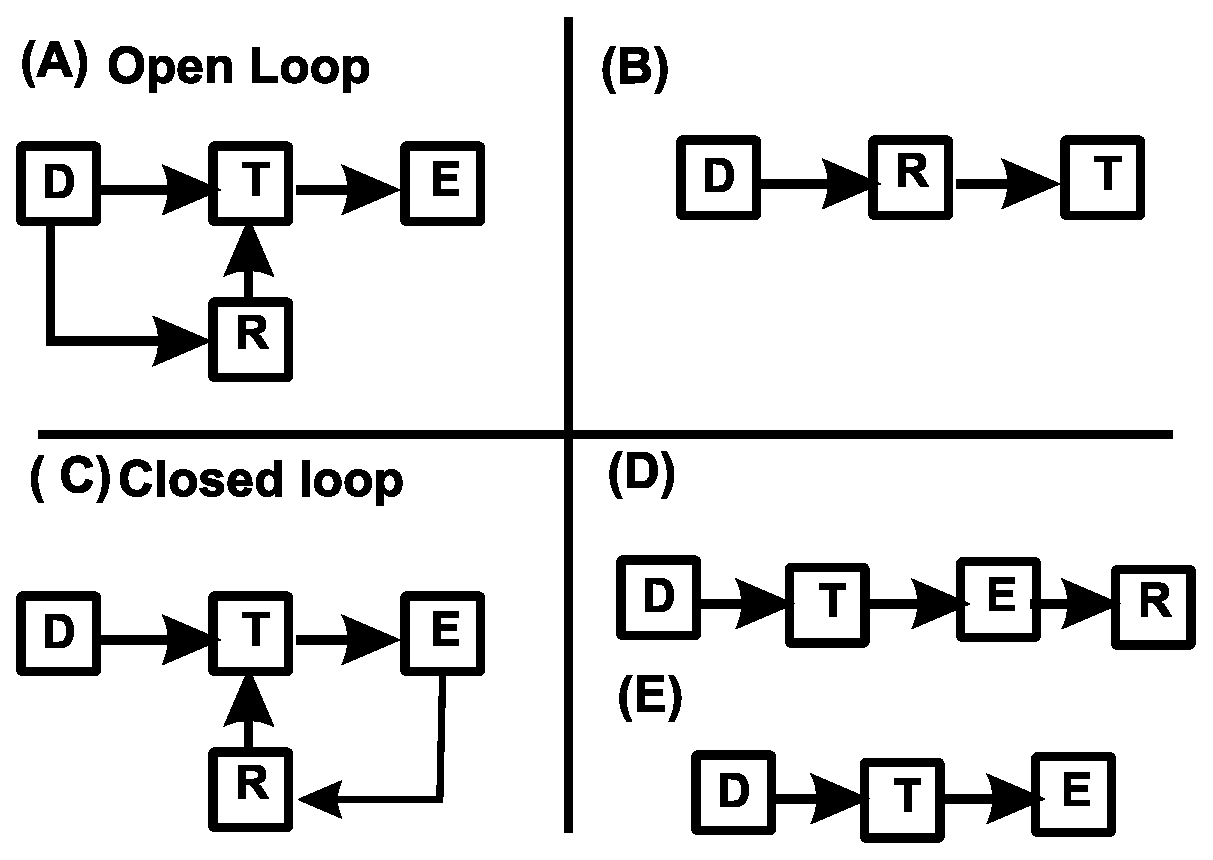
\includegraphics[width=0.6 \textwidth]{ashby/figure-1}
\caption[Ashby requisite variety]{Ashby law of requisite variety applied 
to the open loop case (A),(B) and the closed loop case (C),(D).
\label{fig:infotheory:ashby-model}
}
\end{center}
\end{figure}

Figure \ref{fig:infotheory:ashby-model}(C)(D) describes how the disturbance is absorbed by the regulator
 and the environment to keep a desired state in a closed loop configuration.

The problem of regulation is defined as follows: 
given E,$\eta$, T, and D, to form the mechanism R so that R and T, coupled, 
act to keep E within $\eta$.

\subsection{Direct regulation}
Ashby described direct regulation as a control strategy similar to what engineers
call open loop control.
The update rule for the direct regulation of Figure \ref{fig:infotheory:ashby-model}(A) follows:
\begin{itemize}
 \item D generates a disturbance $d(t)$
 \item $d(t)$ is the input to R which outputs $r(t)$
 \item the 2 values $d(t),r(t)$ are inputs to $T$ that produces $e(t)$
 \item the value $e(t)$ is a state in $E$ which can be a desired or non desired state
\end{itemize}
In the animal world, regulations in simple animals are direct: the organism reacts to the disturbance $D$ before it affects $E$.
A good example is in the life cycle of frogs: tadpoles reacts to a touch stimulus (for example
when a person poke them with a finger) with a swimming reaction opposite to the
direction of the stimulus.
After some time the tadpole will stop swimming: there is no way for the animal
to check if the disturbance was still there.

Most often in the animal world, the R's action cannot be completed before the output of T
is known: the regulator does not know the disturbance directly but only through
the environment or after the organism has experienced the disturbance.


\subsection{Closed loop regulation}
The closed loop regulation is defined when R receives its input from E and not from T
as in Figure \ref{fig:infotheory:ashby-model}(C).
The regulator does not receive directly the disturbance but only after it passed
the environment or the organism.

\begin{figure}
\begin{center}
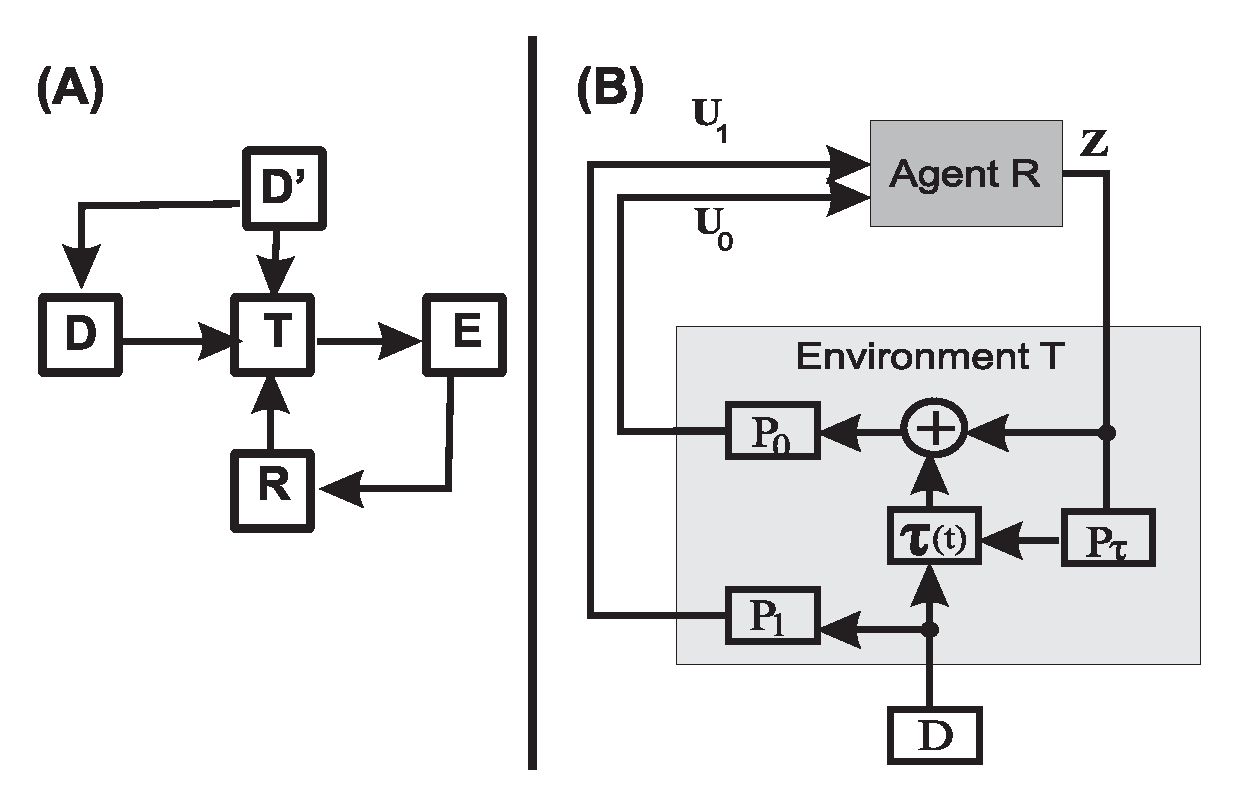
\includegraphics[width=0.8\textwidth]{ashby/figure-3}
\caption[Ashby law in predictive controllers]{
Ashby law of requisite variety applied to the ICO learning controller
\label{fig:infotheory:ashby2}}
\end{center}
\end{figure}

The special case of a predictive controller was not considered by Ashby and therefore
it will be necessary to formulate the necessary conditions for learning.
A possible extension of the Ashby's variety for the ICO controller is in Fig. \ref{fig:infotheory:ashby2}
on the right side there is the ICO controller of the robot and on the left side
there is the corresponding machine state model.
In Fig. \ref{fig:infotheory:ashby2}(A) the disturbance $D'$ is a predictor of $D$ and goes
through the environment $T$ affecting the essential variables $E$ of the controller.
In Fig. \ref{fig:infotheory:ashby2}(B) the diagram of the ICO controller 
This novel approach to predictive controllers is going to be investigated in Section \ref{Chapter8:Predictive Performance}.
In the rest of this section, the original formulation of Requisite Variety is 
introduced.

\subsection{The law of requisite variety}
Please note that with the same notation D,E,R,T,F in the diagrams we refer to
 the determinate or indeterminate (Markovian) closed transformation whose
allowed states are present in the corresponding domains.
\textbf{Definition of regulation:} an organism is a perfect regulator if
is able to keep the essential variables in a desired set $\eta$ in spite
of the disturbances.
\textbf{Regulation blocks the flow of entropy: } if F is a regulator, the insertion
of F between D and E decreases the variety that is transmitted from D to E.
How do we measure the performance of R as a regulator?
\textbf{The function of the regulator R is to reduce the entropy that is transmitted
 from D to E allowing the organism to be in the $\eta$ partition of desired states.}
Thus if F is missing the organism will likely experience the entire set $E$, with
a variety $H(E)$ but when F is introduced, the variety will be reduced to $H(\eta)<H(E)$.
Thus a perfect regulator will prevent the organism from knowing in what state the
disturbance was: the information channel that goes from the disturbance to the
essential variables is blocked totally by the regulator.

The law of requisite variety in terms of Shannon's entropy:
\begin{quotation}
The law of requisite variety says that R's capacity as a regulator cannot
exceed R's capacity as a channel of communication.
It can be formulated in Shannon's terms assuming that: $D$ is the noise that is
 being transmitted to $E$ the essential variables of the organism by means of $T$
the environment, $R$ the regulator is a correction channel whose input is $D$ and
whose output is $T$ whose role is to reduce the variety in the $E$ channel.
In an ideal case $H(E)=0$ such that $H(D)=H(R)$, the regulator must have
the same variety as the disturbance. 
\end{quotation}

\subsection{First law of requisite variety}
Let $D,R$ and $E$ are three random variables.
Hypothesis: when $R$ is given, the entropy of E cannot be less then that of D: $H(E|R)\geq H(D|R)$.
Then the minimum entropy of E is $H(D)+H(R|D)-H(R)$:
\begin{equation}
H(E)\geq H(D)+H(R|D)-H(R) \label{variety:eq:minh}
\end{equation}
\paragraph{Corollary 1:}
if R is a determinate function of D: $H(R|D)=0$, the minimum entropy of E is $H(D)-H(R)$.
The first law of requisite variety says that E's entropy can only be reduced by
 an equal increase in R's variety.
Proof:\\
For the chain rule of entropy:
\begin{equation}
H(R,D)=H(D)+H(R|D)=H(R)+H(R|D)
\end{equation}
substitute $H(E|R)$ for $H(D|R)$ in previous equation gives:
\begin{eqnarray}
H(D)+H(R|D) \leq H(R)+H(R|E)\\
H(D)+H(R|D) \leq H(R,E)\\
H(R,E) \leq H(R)+H(E)\\
H(D) +H(R|D)\leq H(R)+H(E)\\
H(E) \geq H(D) +H(R|D)-H(R)
\end{eqnarray}
The corollary was demonstrated in \citet{Ashby1956:IntroCybernetics}.

\subsection{Second law of requisite variety}
Let D,R and E be three random variables.
Hypothesis: when $R$ is given, the entropy of E cannot be less then that of
 D minus a constant K: $H(E|R)\geq H(D|R)-K$.
Then the minimum entropy of E is $H(D)+H(R|D)-H(R)+K$:
\begin{equation}
H(E)\geq H(D)+H(R|D)-H(R)+K
\end{equation}
The constant K is here used to model the ``handicap'' of the organism.





\chapter{Research work \label{Chapter:Work}}


\section{Introduction: Social Modelling of Artificial Agents}
\label{Chapter4:Social adaptation}
The aim of this section is to develop an Agent Based Model which satisfies the
autopoietic property of Social Systems as introduced in the previous
section \ref{Chapter1:SocialSystemTheory}.
The assumption here is that in an Artificial Society
subsystems are formed to reduce uncertainty.
Uncertainty is faced by agents when learning in their environment.
The simplest learning algorithm is an appropriate reflex which
guides the agent from or to a certain object, for example a wall or
food, as described in the previous section \ref{Intro:Braitenberg}. Learning enables the agent to
anticipate reflexes and to generate anticipatory behaviour as discussed in the previous 
section \ref{Introduction:NeuralSystem}. This, however, poses a problem because
when all agents learn, they change their behaviour all the time which
renders them more and more unpredictable to each other \citep{Luhmann95}.
\citet{Luhmann95} proposed that the creation of subsystems will overcome this
problem. Within these subsystems, agents perform more predictably, by
reducing their behavioural complexity. These subsystems are formed by
adaptive communication between the agents which seems to be essential to form
such subsystems.
Both the behaviour and communication is learned by the agent and is not imposed
on the agent.
The goal or motivation of each agent is to collect food, keep it and eat it until
consumed. Every agent broadcasts its hunger state, which can be used by other
agents, into the world.
This results in two subsystems where agents in the
first collect food and in the latter steal food from others.
The section is structured in this way: description of the agents, world and signals involved,
the learning rule used, agents' behaviours, sub-system formation
and effects of different communication strategies followed by a conclusion.

\subsection{Methods: A Model of the World}
\label{WorldModelSim}
The simulation model is composed of a 2 dimensional world bounded by walls.
It contains two different objects: agents and food sources.
The agents, referenced by their position as $a_{j}(t)$,where $a_{j}$
has 2 components (x,y coordinates indexed by $a_{j,x}$ and $a_{j,y}$),
with $j=1,..,N$. Agents move with a differential drive system named after
Braitenberg \citep{Braitenberg84}.
Food sources are disks located at fixed position $f_{j}(t)$ with $j=1,...,M$.
They can produce constant food or limited food.

\begin{figure}[htbp]
\begin{center}
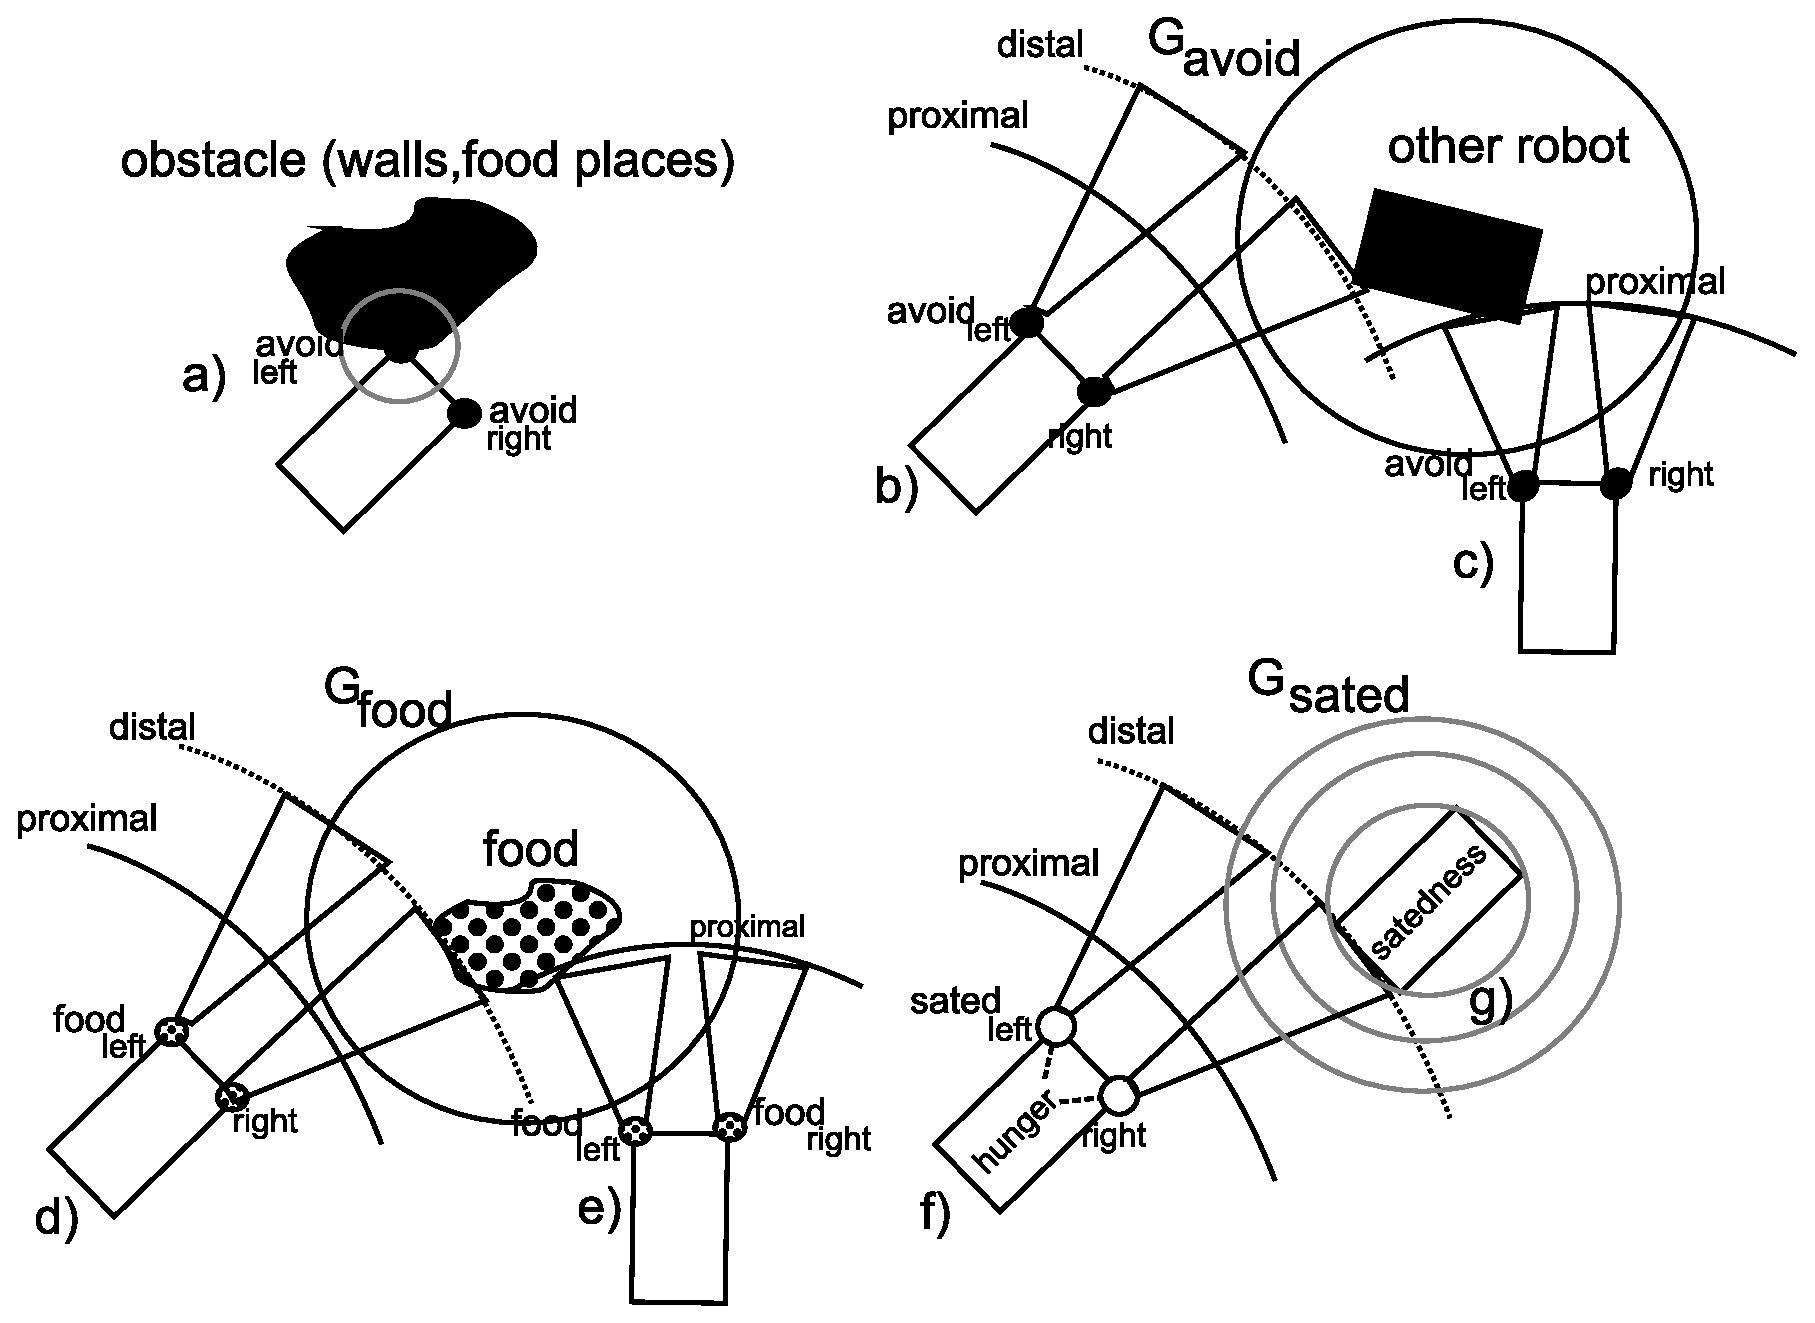
\includegraphics[scale=0.4]{figures/socialadapt/RobotScenario.eps}
\end{center}
\small{
\caption[Social computational model]{Overview of the different signals used in this simulation. 
Circles labelled with G (avoid,food,sated) represent uniform potential fields, circles on 
the robot's front are input sensor, cones irradiating from them represent the field of view 
of sensors, proximal and distal lines represent sensors range. Case a): an agent touches 
a food source or a wall with its proximal left avoidance sensor $avoid_{left,prox}$, 
a proximal signal is generated. Case b): an agent reads the potential field $G_{avoid}$ 
produced by another, with its right distal sensor $avoid_{right,dist}$. Case c): 
an agent reads the potential field $G_{avoid}$ produced by another agent, with 
both left and right proximal sensors $avoid_{left,prox},avoid_{right,prox}$. 
Case d): an agent reads the potential field $G_{food}$ produced by a food source, 
with its right and left distal sensors $food_{right,dist},food_{left,dist}$. 
Case e): an agent reads the potential field $G_{food}$ produced by a close 
food source, with both left and right proximal sensors $food_{left,prox},food_{right,prox}$. 
Case f,g): a hungry agent f (with $Hunger=1$) reads the satedness signal $G_{sated}$ 
produced by the sated agent g. \label{fig:sensors}
}}
\end{figure}

Agents have different sensors which enable them to sense
obstacles, other agents' presence and others' broadcasted state of satedness, at
different ranges (proximal and distal see Fig. \ref{fig:sensors}).
Every object labelled with a certain index $j$ produces a signal carried by a
uniform potential field $G_{j,type}$ with a limited range, which is sensed
by the corresponding sensor type (type can be avoid,food or sated).
The potential field $G_{j,type}$ is described by the equation of a circle which is centered
on $x_0,y_0$ with a $r$ radius:
\begin{equation}
(x-x_0)^2+(y-y_0)^2=r^2 \label{eq:circle}
\end{equation}
Every geometric point $x,y$ including a sensor or object which falls inside 
the circle $G_{j,type}$ assumes a unitary value.
The signals from the proximal sensors ($x_{0}$) are originally used to drive
the agents reflexes which can either be avoidance or attraction. The signals
from the distal sensors are used for learning so that the agent is able to
generate anticipatory reactions instead of the reflexes as introduced in section \ref{Introduction:NeuralSystem}.

In the next section I am going to describe the learning algorithm enabling the agent to
replace the reflexes with the predictive actions.
Once the learning algorithm is described, I will describe the different reflexes and possible
anticipatory reactions.
\subsection{Methods: ICO learning module}
\label{Section:ICOlearning}
The input correlation learning rule of \citet{Porr2006ICO} is a Hebbian learning rule,
it is unsupervised and performs a confounded correlation between a predefined reflex signal
($x_{0}$) and a reflex predicting signal ($x_{1}$). Hence, this learning
algorithm identifies and exploits causalities between temporal
sequential signals.
The ICO learning block was chosen because it is one of the simplest,fastest and computationally 
efficient approach to temporal learning.
It can also be easily implemented in analogic and digital systems without any
 particular modifications.

\begin{figure}[htbp]
\begin{center}
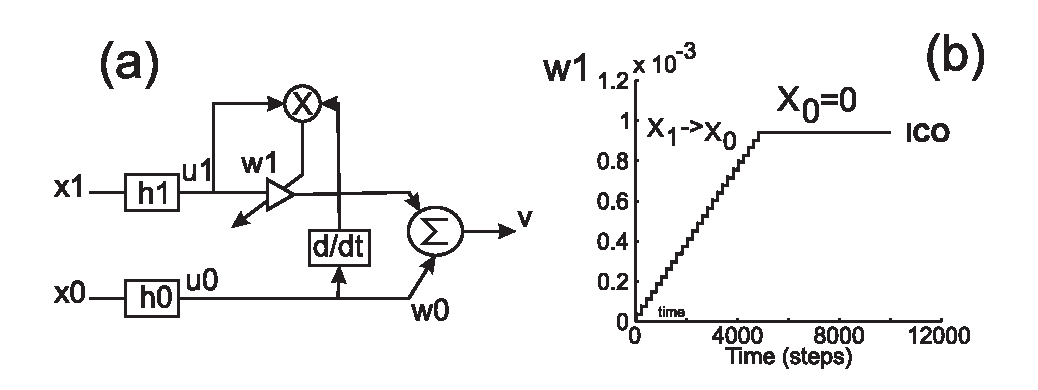
\includegraphics[scale=0.5]{figures/socialadapt/ico.eps}
\caption[Agent learns with the ICO learning]{Figure (a) shows the ICO learning basic
block composed by 2 inputs $x_{0},x_{1}$ filtered by $h_{0},h_{1}$ and the output $v$.
Figure (b) shows the weight change of $w_{1}$ during time. At the beginning $w_{1}=0$,
then for 5000 simulation steps $x_{1}$ anticipates $x_{0}$ and the $w_{1}$ grows until 1.0.
After 5000 simulation steps reflex is suppressed $x_{0}=0$ and $w_{1}$ stabilises to $1 \cdot 10^{-3}$.
\label{fig:ico}}
\end{center}
\end{figure}

Figure \ref{fig:ico} shows the ICO learning block which has two inputs $x_{0}$,$x_{1}$
from the agent's sensor that are filtered by low pass filters $h_{0},h_{1}$:

\setlength{\arraycolsep}{0.0em}
\begin{eqnarray}
&h(t)=&\frac{1}{b}e^{at}sin(bt) \label{eq:1}\\
&a   =&-\pi \frac{F}{Q} \label{eq:F}\\
&b   =&\sqrt{(2\pi F)^2 -a^{2}} \label{eq:Q}
\end{eqnarray}
\setlength{\arraycolsep}{5pt}

$F$ is the oscillation frequency and $Q$ the quality factor. The low passed
signals $u_{i}(t)$ are transferred with weight $w_{i}$ to the output
neurons (for more details see Appendix \ref{app:appendixICO}).

\setlength{\arraycolsep}{0.0em}
\begin{eqnarray}
u_1 &=& h \ast x_1 \\
u_0 &=& h \ast x_0
\end{eqnarray}
\setlength{\arraycolsep}{5pt}
where $\ast$ is the convolution operation which implement the filtering operation.
In the output neuron the output $v(t)$ is calculated by
summing up all incoming signals according to their weights:
\begin{equation}
v(t)=w_{0}\cdot u_{0}+w_{1}\cdot u_{1}
\end{equation}
which represent the input for the motor system.
The unsupervised character of the ICO learning rule is reached by
the synaptic weight $w_{1}$ to be adapted by the weight
change rule:
\begin{equation}
\frac{\partial w_{1}}{\partial t}=\mu u_{1} \frac{\partial u_{0}}{\partial t}
\end{equation}
The weight change is dependent on the derivative of the reflex input
signal $u_{0}$, the input signal $u_{1}$ and a
learning rate $\mu$. The
learning rule has been shown to be useful for avoidance and attraction
mechanisms and has fast and stable convergence.


\subsection{Methods: agent controller}
For the sake of simplicity, the agent's neural controller is analysed block
by block according to the requested behaviours (avoidance and attraction)
in Figs. \ref{fig:avoidance},\ref{fig:attractionAgent},\ref{fig:attraction}.
The core is composed of two ICO neurons, labelled with L-eft and R-ight,
connected to the motor outputs left and right. Both ICO neurons have a
constant bias input B with weight 4.0 that makes the robot move forward
if inputs are absent. Rectangular blocks labelled with L,R are low pass
filters, with parameters $F,Q$ referred to equations \ref{eq:F},\ref{eq:Q}.
Synaptic weights of the ICO block in Fig. \ref{fig:ico}(a) are labelled with
$W$ capital letter and two pedex that indicate the weight type
(predict is learned and reflex is fixed) and the synapse position (left,right).
ICO neurons have recurrent synaptic connections, labelled as
$W_{R2L},W_{L2R},W_{selfR},W_{selfL}$ to implement a hysteresis effect,
which causes the controller to not instantly follow signals as in \citet{Hulse2004,Paseman2002}).
It means reactions on an incoming signal are time shifted. This is useful to enable agents to escape from acute angles: if
an agent incurs in an concave acute angle and has not a hysteresis mechanism,
will get stuck inside, turning left and right alternatively.

\subsection{Methods: avoidance behaviour}
Agents and walls are obstacles. Agents produce obstacle
signals (see Fig.\ref{fig:sensors} (a) for obstacles and
Fig.\ref{fig:sensors} (b),(c) for other agents). Every agent $a_{j}(t)$ has a
potential field associated (see Eq.\ref{eq:circle}):
\begin{equation}
Gavoid_{j}(t)=G(x-a_{j,x}(t),y-a_{j,y}(t)).
\end{equation}
that is sensed by the corresponding inputs of other agents $a_{k}(t)$ (with $k\neq j$)
labelled as $avoid_{left,right}$. Walls and food sources
do not produce $G_{avoid}$, so that agents sense them using proximal signals that are
generated by collisions: when 2 distinct agents $j$ and $l$ collide at time $t_{0}$, such
that $||a_{j}(t)-a_{l}(t)||_{2}<D$ ($D$ is the radius of the
agent) an impulse is produced at $avoid_{l,r}$.
\begin{figure}[htb]
\begin{center}
\includegraphics[scale=0.45]{figures/socialadapt/avoidance.eps}
\end{center}
\vspace*{4pt}
\small{
\caption[Avoidance learning behaviour]{Avoidance network: ICO left and right are
two neurons implementing the ICO learning rule, their output is a sigmoid and
is connected (after normalization into $[v_{min},v_{max}]$) to the motor speed commands.
Grey triangles represents distal inputs, while white triangles represent proximal inputs.
The learned synaptic weights are associated to the distal synapses (thick lines) while
the fixed are associated to the proximal synapses (dotted lines).
To produce a retraction behaviour left and right weights must be different
such that
$W_{predict,L}>W_{predict,R}$ and $W_{reflex,L}>W_{reflex,R}$, if
$W_{predict,L}=W_{predict,R}$ and $W_{reflex,L}=W_{reflex,R}$ robot
will just go back without turning.\label{fig:avoidance}}}
\end{figure}
The neural controller for the avoidance behaviour is shown in
Fig. \ref{fig:avoidance} (see also \citep{Stamm2006}), every ICO neuron (left and right)
computes the following operations:

\begin{eqnarray}
ICO_{L}(t)&=B-h \ast avoid_r\cdot W_{reflexL}-h \ast avoid_{dist,r}\cdot W_{predictL}\\ \nonumber
	  &+W_{selfL}\cdot ICO_{L}(t-1) + W_{L2R}\cdot ICO_{R}(t) \label{eq:ICO:L1} \\ 
ICO_{R}(t)&=B-h \ast avoid_l\cdot W_{reflexR}-h \ast avoid_{dist,l}\cdot W_{predictR}\\ \nonumber
	  &+W_{selfR}\cdot ICO_{R}(t-1) + W_{R2}\cdot ICO_{L}(t)  \label{eq:ICO:R1}
\end{eqnarray}

The parameters used for the weights, the bias and the recurrent connections are
reported in the Appendix sections \ref{Appendix:HysteresysValue},\ref{Appendix:simulation}.
The recurrent connections between the left and right ICO neuron, are necessary
to implement a push-pull behaviour so that when the robot synchronously activates
both the left and the right input, only one ICO neuron will dominate thus evoking
a turn-back response. 
Connections between input synapses and ICO neurons (motor neurons) are
negative to evoke a retraction. 
The motor output is calculated with a sigmoid activation function on the ICO neuron
membrane as follow:

\begin{eqnarray}
V_{L}&=& \frac{1}{1+e^{-ICO_{L}}}\\
V_{R}&=& \frac{1}{1+e^{-ICO_{R}}}
\end{eqnarray}

The weight update learning rule is calculated for the weigts:

\begin{eqnarray}
\frac{\partial W_{predict,L}}{\partial t}&=& \mu \cdot avoid_{dist,l} \frac{\partial avoid_{l}}{\partial t}\\
\frac{\partial W_{predict,R}}{\partial t}&=& \mu \cdot avoid_{dist,r} \frac{\partial avoid_{r}}{\partial t}
\end{eqnarray}


\subsection{Methods: Agents and satedness communication}
Every agent has an internal state: hunger and its complementary satedness.
\begin{figure}[htbp]
\begin{center}
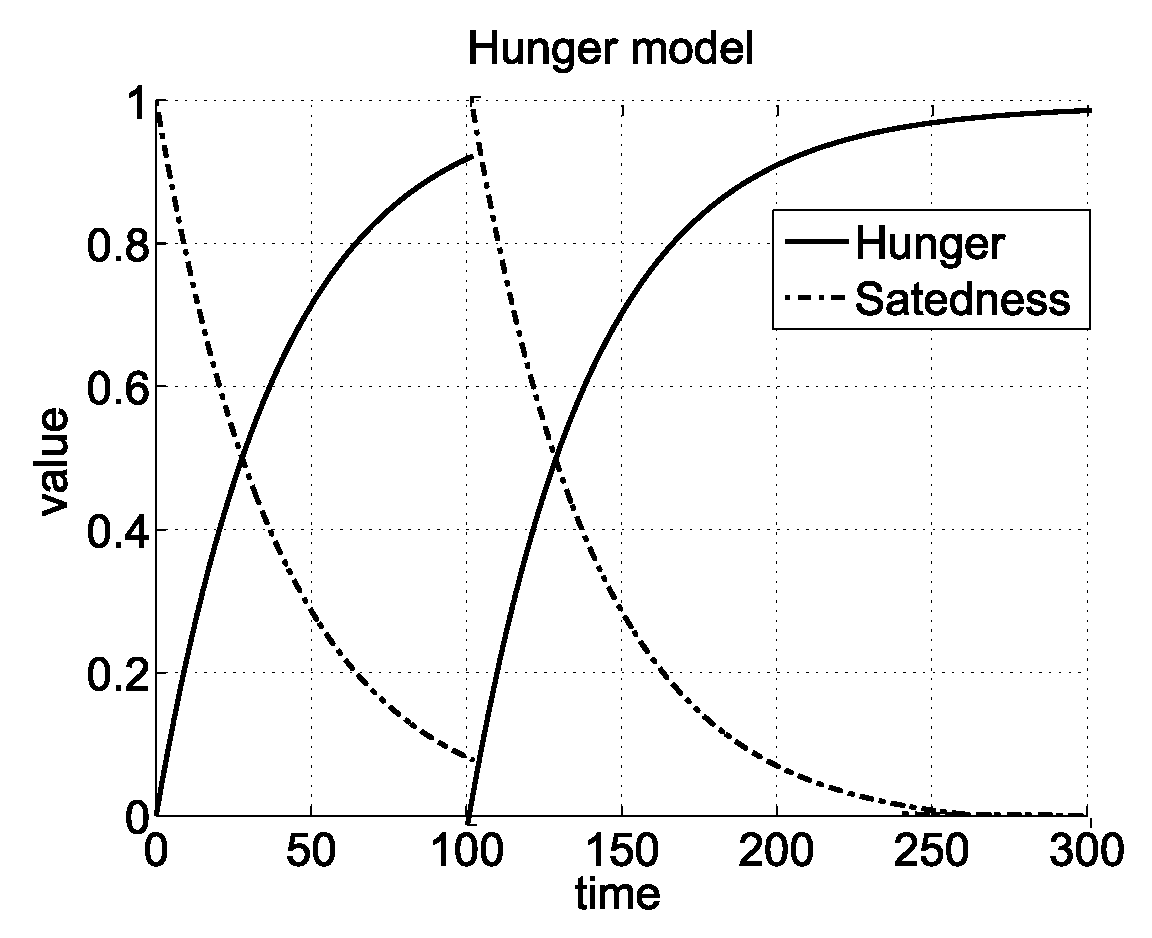
\includegraphics[scale=0.3]{figures/socialadapt/hungersatshift.eps}
\end{center}
\vspace*{4pt}
\caption[Energy state or hunger of the artificial agent]{
Hunger state in function of time. At time step 100 the agent touches a
food place, thus its hunger state is reset to 0 and so its complementary
satedness to 1. \label{fig:hunger}}
\end{figure}

The energy level of each agent is an exponential function of time:
\begin{equation}
H_{sated}(t)=
  \begin{cases}
   e^{-t/\tau_{starv}} & \text{if } t \geq t_b \\
   0       & \text{if } t < t_b
  \end{cases}
\label{eq:satstate}
\end{equation}
and complementary its hunger state is:
\begin{equation}
H_{hunger}(t)=1-H_{sated}(t)
\end{equation}
where $\tau_{starv}$ is the starvation factor and $t_b$ corresponds to the moment
when an agent touches a food source:
\begin{equation}
|food_{l,prox,d_{1}}(t_{b})+food_{r,prox,d_{1}}(t_{b})|>\theta_{F}.
\label{eq:touchfood}
\end{equation}
or touches a sated agent (see Fig. \ref{fig:hunger}):
\begin{equation}
|sated_{l,prox,d_{1}}(t_{b})+sated_{r,prox,d_{1}}(t_{b})|>\theta_{A}.
\label{eq:touchagent}
\end{equation}
and agent is touching an obstacle
\begin{equation}
|avoid_{prox,l}(t_{b})+avoid_{prox,r}(t_{b})|>\theta_{O}.
\end{equation}
where $\theta_{F},\theta_{A},\theta_{O}$ are thresholds for food, agents and
obstacles respectively.
In Fig. \ref{fig:attractionAgent}, internal state $H_{hunger}(t)$ is multiplied
for $food(t)$ (left,right and proximal,distal) and $sated(t)$ (left, right and proximal, distal).

Satedness internal state of agent $a_{i}$, is broadcasted to other agents
$a_{k}(t)$ (with $k\neq j$) by means of a potential field (see Fig.\ref{fig:sensors}(g) and Eq.\ref{eq:circle}):
\begin{equation}
G_{i,sated}(t)=H_{sated}(t) \cdot G(x-a_{i,0},y-a_{i,1}).
\label{eq:gsated}
\end{equation}
Agent $a_{k}(t)$ senses $G_{i,sated}$ (see Fig.\ref{fig:sensors} (f)) with 2
reflexive inputs $sated_{l,prox,d_{1}}(t)$ and 
$sated_{r,prox,d_{1}}(t)$ whose difference feeds the reflexive input:
\begin{equation}
x_{0}(t)=sated_{l,prox,d_{1}}(t) - sated_{r,prox,d_{1}}(t).
\end{equation}
and as predictive $sated_{l,prox,d_{2}}(t),sated_{r,prox,d_{2}}(t)$ whose
difference feeds the predictive input:
\begin{equation}
x_{1}(t)=sated_{l,dist,d_{2}}(t) - sated_{r,dist,d_{2}}(t).
\label{eq:foodagentpredictive}
\end{equation}
where $d_{2}>d_{1}$.
The equations \ref{eq:ICO:L1},\ref{eq:ICO:R1} of the ICO neurons are added to the
following synaptic inputs:

\begin{eqnarray}
ICO_{L}&=&-h \ast ( x_0 \cdot H_{hunger}) \cdot W_{reflex,A,L} \\ \nonumber
       & &-h \ast ( x_1 \cdot H_{hunger}) \cdot W_{predict,A,L} \label{eq:ICO:L2}\\
ICO_{R}&=& h \ast ( x_0 \cdot H_{hunger}) \cdot W_{reflex,A,R} \\ \nonumber
       & &+h \ast ( x_1 \cdot H_{hunger}) \cdot W_{predict,A,R} \label{eq:ICO:R2}
\end{eqnarray}
The reason for the sign inversion for the weights is that the inputs
are differential and thus is necessary for the left ICO neuron have
an input of opposite sign to the right ICO neuron.
The weight update rule this time is:
\begin{eqnarray}
\frac{\partial W_{predict,A,L}}{\partial t}&=& \mu \cdot x_1 \frac{\partial x_0}{\partial t}\\
\frac{\partial W_{predict,A,R}}{\partial t}&=& \mu \cdot x_1 \frac{\partial x_0}{\partial t}
\end{eqnarray}

Inputs for the attraction task are shown in Fig. \ref{fig:attractionAgent}.
When for example:  $x_{0}(t)>0$ implies that a sated agent is on the left
$sated_{l,prox,d_{1}}(t)>0$, the neural controller produces $v_{L}<v_{R}$,
agents turns left until $x_{0}(t)=0$ that means either $x_{0}(t)=x_{1}(t)$
(a sated agent is in front) or $x_{0}(t)=x_{1}(t)=0$ (no sated agent in front).
A hungry agent, is producing $G_{i,sated}(t)=0$ therefore other agents will be
 repelled since it is emitting only the $G_{avoid}$ signal.

\paragraph{Aggressive agents}\label{eq:aggressive}
If one wants to make an agent more aggressive  $H_{sated}(t)$ can be multiplied for the
distal sensors $avoid(t)$ left, right (in Fig.\label{fig:avoid} the $H_{hunger}$
block can be introduced after each of the grey triangles). It implies that when
an agent is not sated, it will ignore the obstacle signal $G_{avoid}$
produced by the other agent.

\begin{figure}[htb]
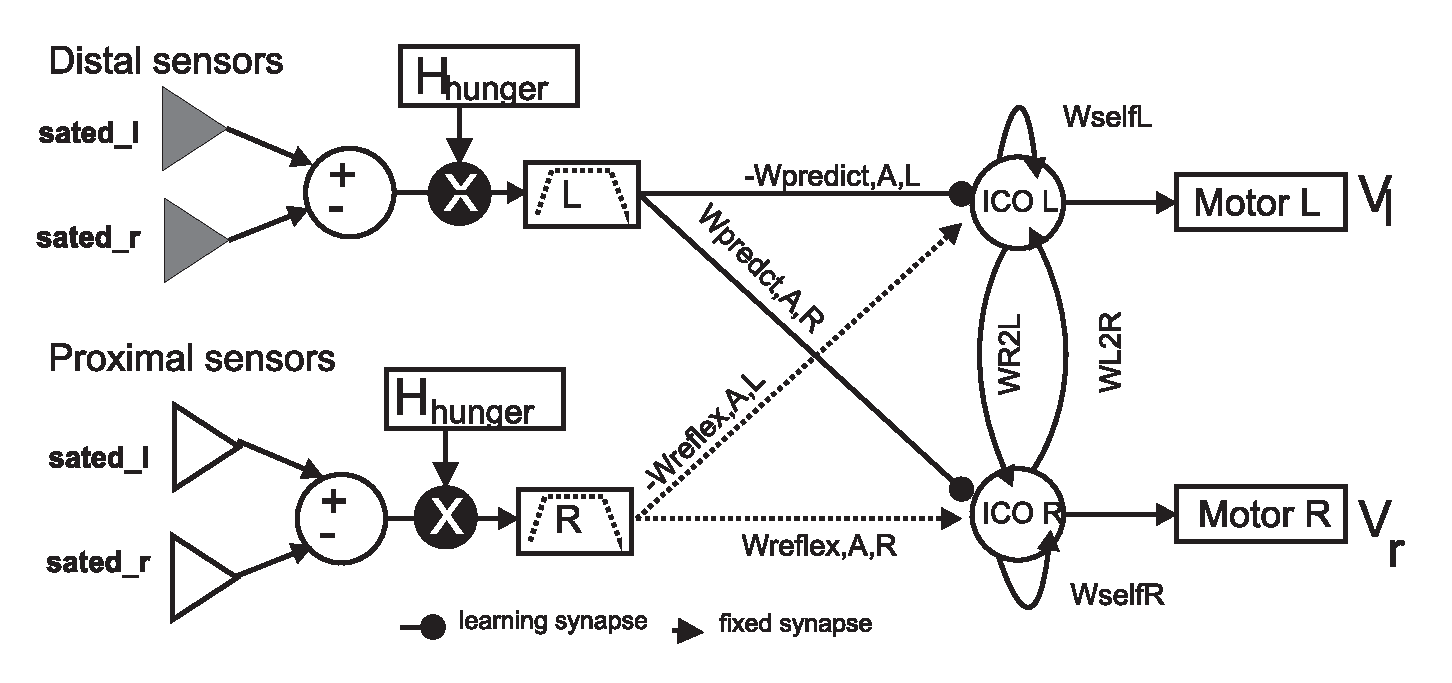
\includegraphics[scale=0.4]{figures/socialadapt/attractionAgent.eps}
\small{
\caption[Attractive behaviour for other agents]{
Attraction toward sated agents:two more inputs are added to the ico neurons.
Grey triangles represents distal inputs, while white triangles represent
proximal inputs. The learned synaptic weights are associated to the distal
synapses (thick lines) while the fixed are associated to the proximal
synapses (dotted lines). Synaptic weights must be equal in module and
opposite in sign $|W_{predict,A,L}|=|W_{predict,A,R}|$ and
$|W_{reflex,A,L}|=|W_{reflex,A,R}|$  where $A=agent$.
Hunger internal state is multiplied for proximal and distal
input difference \label{fig:attractionAgent}}
}

\end{figure}


\subsection{Methods: Food attraction}
Every food source $f_{j}(t)$ with $j=1,...,M$ produces the signal
(see Fig.\ref{fig:sensors} (d),(e) and Eq.\ref{eq:circle}):
\begin{equation}
G_{j,food}=G(x-f_{j,x},y-f_{j,y}).
\label{eq:food}
\end{equation}
which is sensed by agents $a_{i}$ by the inputs labelled as
$food_{left,right}$ (see Fig.\ref{fig:sensors} (d),(e)).
\paragraph{Constant food production}
Every food source contains a constant amount of food which means $G_{j,food}$
is always emitted.
\paragraph{Limited food production}
Every food source contains a limited amount of food modelled by the variable $q$ that
 is decremented every time an agent touches the food place at $t_{b}$:
\begin{equation}
q_{j}(t_{b}+1)=q_{j}(t_{b})-\theta q.
\label{eq:qfood}
\end{equation}
where ($\theta q$ is fixed).
When $q_{j}=0$ the food source $j$ is exhausted and food signal is suppressed $G_{j,food}=0$.
After a random period the food source is restored $q_{j}=1$.
\begin{figure}[htb]
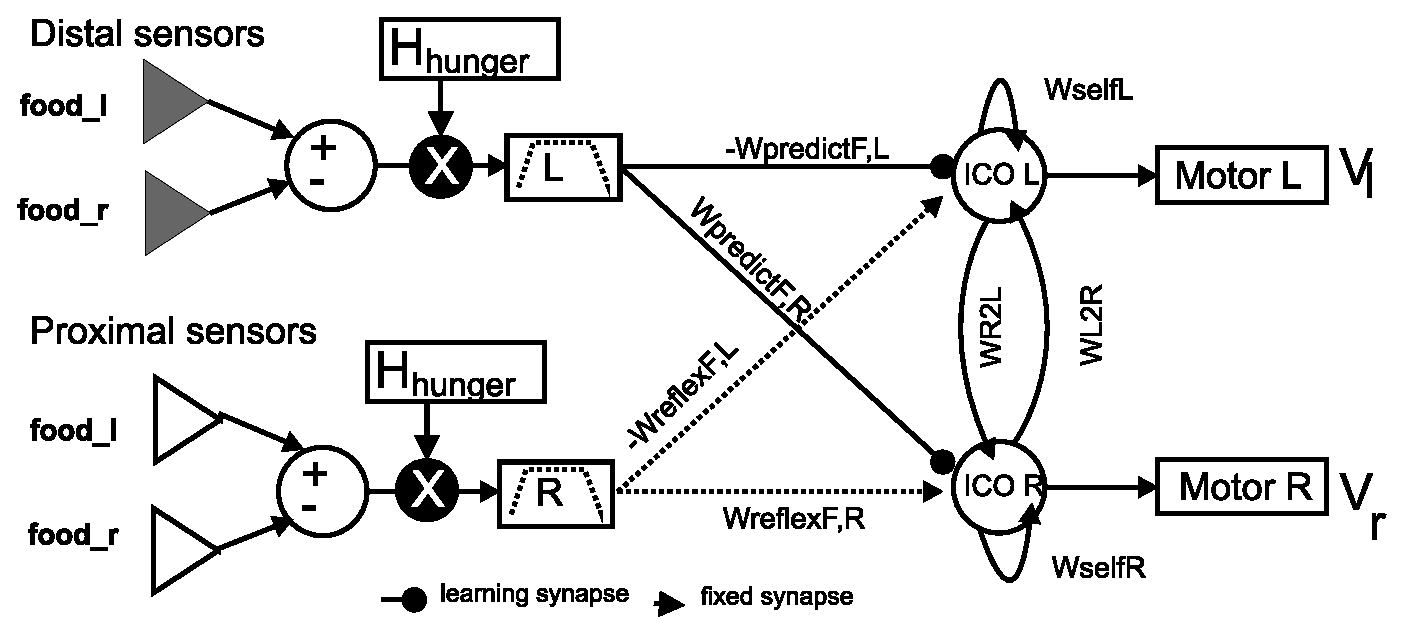
\includegraphics[scale=0.4]{figures/socialadapt/attractionFood.eps}
\vspace*{4pt}
\small{
\caption[Attraction learning behaviour for food]{Attraction toward food:
two more inputs are added to the previous network. Grey triangles represents
distal inputs, while white triangles represent proximal inputs.
The learned synaptic weights are associated to the distal synapses (thick lines)
 while the fixed are associated to the proximal synapses (dotted lines).
Synaptic weights in the attraction task must be equal in module and opposite
in sign: $W_{predict,F,L}=W_{predict,F,R}$ and $W_{reflex,F,L}=-W_{reflex,F,R}$
where $F=food$ \label{fig:attraction}}
}
\end{figure}

Required inputs for the attraction behaviour are introduced in
Fig. \ref{fig:attraction} (see also \citep{Stamm2006}),
for every ICO neuron an additional reflex is added:
\begin{equation}
x_{0}(t)=food_{l,prox,d_{1}}(t)-food_{r,prox,d_{1}}(t).
\end{equation}
$x_{0}$ it is the difference between the left and right proximal food input sensors.
A predictive input is added:
\begin{equation}
x_{1}(t)=food_{l,dist,d_{2}}-food_{r,dist,d_{2}}(t).
\end{equation}
$x_{1}(t)$ it is the difference between the left and right distal food input sensors.
Thus $d_{2}>d_{1}$ such that the distal food sensor values are
predictive on the proximal food sensors.
The equations \ref{eq:ICO:L2},\ref{eq:ICO:R2} of the ICO neurons are added to the
following synaptic inputs:

\begin{eqnarray}
ICO_{L}&=&-h \ast ( x_0 \cdot H_{hunger}) \cdot W_{reflex,A,L} \\ \nonumber
       & &-h \ast ( x_1 \cdot H_{hunger}) \cdot W_{predict,A,L} \label{eq:ICO:L3}\\
ICO_{R}&=& h \ast ( x_0 \cdot H_{hunger}) \cdot W_{reflex,A,R} \\ \nonumber
       & &+h \ast ( x_1 \cdot H_{hunger}) \cdot W_{predict,A,R} \label{eq:ICO:R3}
\end{eqnarray}
The reason for the sign inversion for the weights is that the inputs
are differential and thus is necessary for the left ICO neuron have
an input of opposite sign to the right ICO neuron.
The weight update rule this time is:
\begin{eqnarray}
\frac{\partial W_{predict,A,L}}{\partial t}&=& \mu \cdot x_1 \frac{\partial x_0}{\partial t}\\
\frac{\partial W_{predict,A,R}}{\partial t}&=& \mu \cdot x_1 \frac{\partial x_0}{\partial t}
\end{eqnarray}

When for example: $x_{0}(t)>0$ implies that food source is on the left, the neural
controller produces $v_{L}<v_{R}$, agent turns left until $x_{0}(t)$ becomes 0.

\subsection{Controller summary}
For clarity Fig. \ref{fig:controllerSummary} contains the simplified but full structure of the controller whereby the two
ICO neurons receive synaptic inputs from each synaptic input described before.
There are a total of twelve inputs because for every behaviour there are left and
right sensors for the distal and proximal case.
Because there are three behaviours, multiplied by 4 makes 12 parallel inputs.
The inputs are then low pass filtered as described before and summed at the 
ICO neuron $\sum$.
The left and right ICO neurons are also responsible for updating the weights
for the predictors.
The output of each ICO neuron is then fed into a sigmoid function which normalizes
the output in the $[-1,1]$ range for controlling the robot motors.

\begin{figure}
\begin{center}
\includegraphics[width=1.0\textwidth]{figures/socialadapt/ControllerSummary}
\end{center}
\vspace*{4pt}
\caption[Full schematic of the controller]{
The robot controller implements the 3 behaviours by using a linear
summation of all the synaptic inputs \label{fig:controllerSummary}}
\end{figure}


\subsection{Broadcasting signal mechanism}
\label{SocialSystem:Broadcast}
The main feature of a social system is the production and use of signals.
Thus each agent can emit the same field in equation \ref{eq:food} in the presence of a food source.
A more detailed discussion about signalling strategies is in the Conclusion section \ref{TheoryOfMind}.
There are only two possible signalling strategies in my model, honest and dishonest
strategies and are going to be described in the following sections.

\subsubsection{Honest food proximal signalling}
In this scenario agents signal the presence of food when they sense it using
the proximal inputs: $G_{food}$ is emitted by an agent when $food_{l,prox,d_{1}}(t)>0$, $food_{r,prox,d_{1}}>0$
and $|food_{l,prox,d_{1}}(t)-food_{r,prox,d_{1}}|<\theta F$ ($\theta F$ as Eq.\ref{eq:touchfood}).
This "genuine" social behaviour might increase the foraging performance of the colony,
but might cost the signaller because it can result in higher robot density and increased
competition and interference nearby the food (i.e. spatial constraints around the food disk:
only 9 agents can forage at same time). Thus, although beneficial to other colony members,
signalling of a food location can constitute a costly act \citep{AnimalSignals} because it
decreases the food intake of signalling robots. With this social rule agents tend to form
lines around the food zones: they are more organized then the previous case.

\subsubsection{Dishonest food proximal signalling}
In this case the agent "cheats" producing non predictable (using a uniform probability
of emitting $p(e)=0.6$) food signals when they are far away from the food zones
($food_{l,dist,d_{2}}=0$ AND $food_{r,dist,d_{2}}(t)=0$) and of course when they
are not sated ($H_{sated}(t)< 0.2$ a threshold). The percentage of cheaters used in the
test was: $10\%,50\%$,and $80\%$. Doing so an agent reduces the competition around the food zones.


\subsection{Results: analysis of formation in different cases}
The following sections contain the most important test cases for our model:
\begin{itemize}
\item general overview about the sub-system property and the food signalling strategies
\item a comparison of the food performance between adaptive communication and non communicative strategy
\item an insight to the honest behaviour with unlimited resources
\item an insight to the honest behaviour with limited resources and environmental changes
\end{itemize}

\subsubsection{Sub-system formation and adaptive communication}
During time agents learn to: avoid obstacles, search for food and search for
other sated agents.
Because all the inputs (see Fig. \ref{fig:controllerSummary}) are used in parallel
and summed linearly for the motor behaviour, the weights will develop independently
from each other in a competitive fashion.
For example when an agent sees a closer agent with food and a food source, the outcome
of the motor behaviour will depend on the weight status for each behaviour.
Thus agents can be classified in 2 classes, seekers and parasites,
according to their weights \footnote{$W_{predict,A}$ is the average
of $|W_{predict,A,L}|,|W_{predict,A,R}|$ and $W_{predict,F}$ is the average of $|W_{predict,F,L}|,|W_{predict,F,R}|$}:
\begin{equation}
\delta_{w,agent}=\frac{|W_{predict,A}(0)-W_{predict,A}(T_{sim})|}{W_{predict,A}(0)}.
\end{equation}

\begin{equation}
\delta_{w,food}=\frac{|W_{predict,F}(0)-W_{predict,F}(T_{sim})|}{W_{predict,F}(0)}.
\end{equation}

where the fraction is used to normalize the weight development, so in summary:
\begin{itemize}
 \item \textbf{An agent is a seeker} $\delta_{w,agent} > \delta_{w,food}$, if it is more
attracted by food places than other sated agents.
\item \textbf{An agent is a parasite} $\delta_{w,agent}\leq \delta_{w,food}$, if it is
more attracted by sated agents than food places.
\end{itemize}
This classification will then be compared to a subjective comparative analysis in
section \ref{Chapter8:PPsocial}.
Sub-system formation is analysed for 2 important test cases:
\begin{itemize}
 \item adaptive communication: the agents learn using both proximal and distal signals
 \item no communication: the agents do no produce the $G_{sated}$ food signal necessary
for the other agents to know whether food is available or not.
\end{itemize}
The non communicative condition does not imply that in Eq. \ref{eq:foodagentpredictive} distal
signals are suppressed but rather that agents will learn only when the neighbouring agent
is enough close to be sensed by the far sensors.
This implicate that learning will be happening still but only when robots are close 
to each other rather than via the broadcast field  $G_{sated}$.
For our simulation, a population of $N=20$ agents is provided with $M=4,10,18$ food sources sequentially.
Population dynamic is observed for a total duration of  $T_{sim}=80000$ (time step $\triangle T=0.01 s$).
Fig.\ref{fig:generalcomparison} resumes a total of 6 test cases: left column considers scarce resources
 ($M=4$ food sources against $N=20$ agents), right column considers abundant resources ($M=18$ food sources against $N=20$ agents).
Each one of them reports the number of seekers (thick line) and parasites (dotted line) in function of time.
The number of seekers $n_{s}(t)$ is complementary to the number of parasites $n_{p}(t)$: 
\begin{equation}
n_{s}(t)+n_{p}(t)=N \label{eq:social:ratio} 
\end{equation}
When the simulation is over $t=T_{sim}$ the ratio is:
\begin{equation}
n_{s}(T_{sim})+n_{p}(T_{sim})=N \label{eq:social:ratiofin} 
\end{equation}

\begin{figure}[htbp]
  \begin{center}
      \subfigure[No food signal, ratio $N=20,M=4$]{
	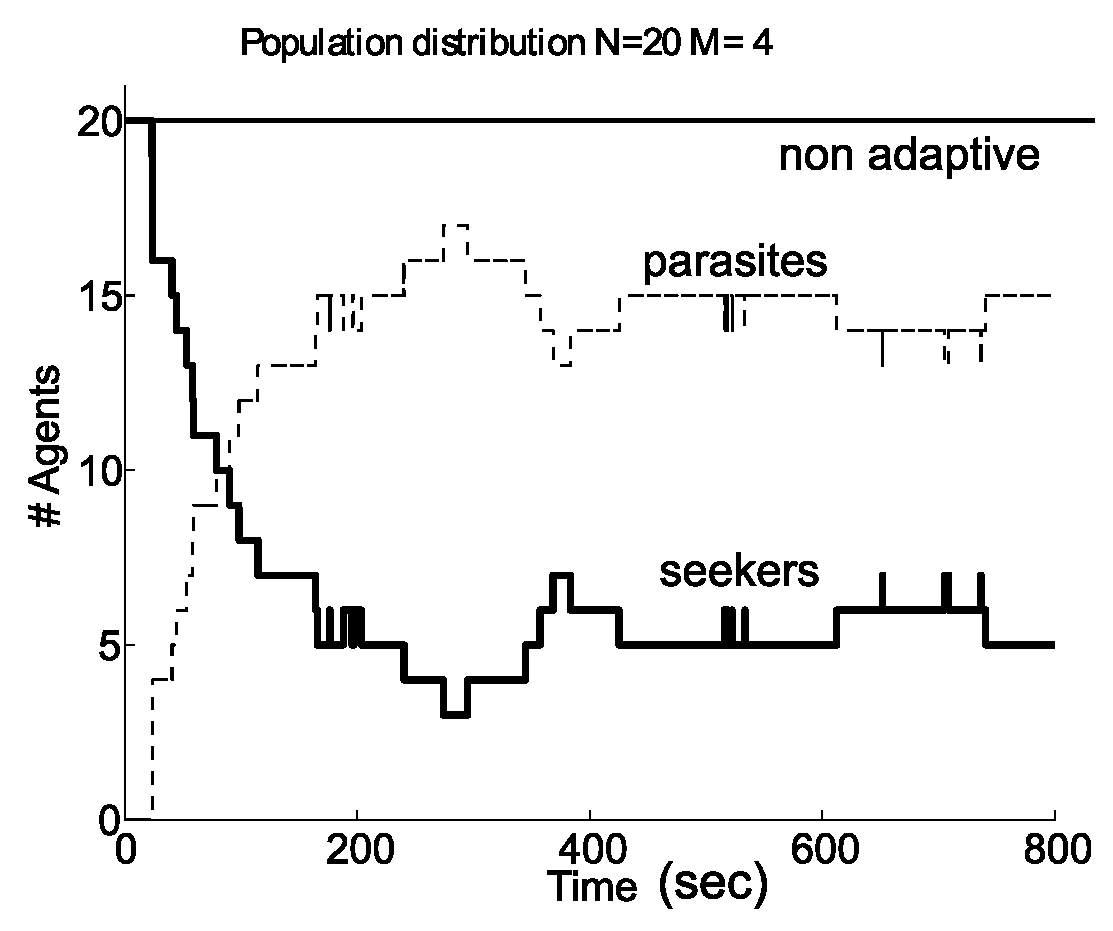
\includegraphics[width=0.4 \textwidth]{figures/socialadapt/nosignal/comm20TO4.eps}}
      \hspace{1pt}
      \subfigure[No food signal, ratio $N=20,M=16$]{
	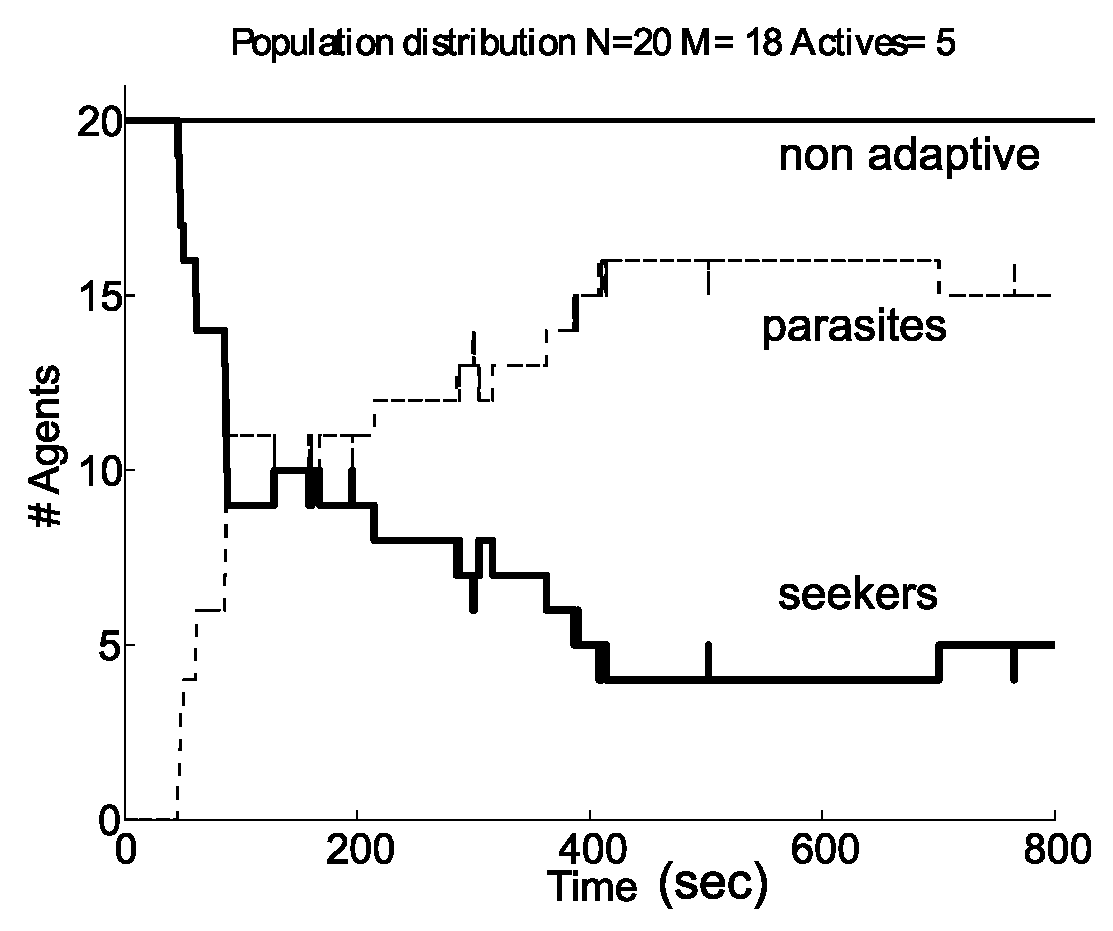
\includegraphics[width=0.4 \textwidth]{figures/socialadapt/nosignal/comm20TO18.eps}}
      \vspace{1pt}
      \subfigure[Honest food signal, ratio $N=20,M=4$]{
	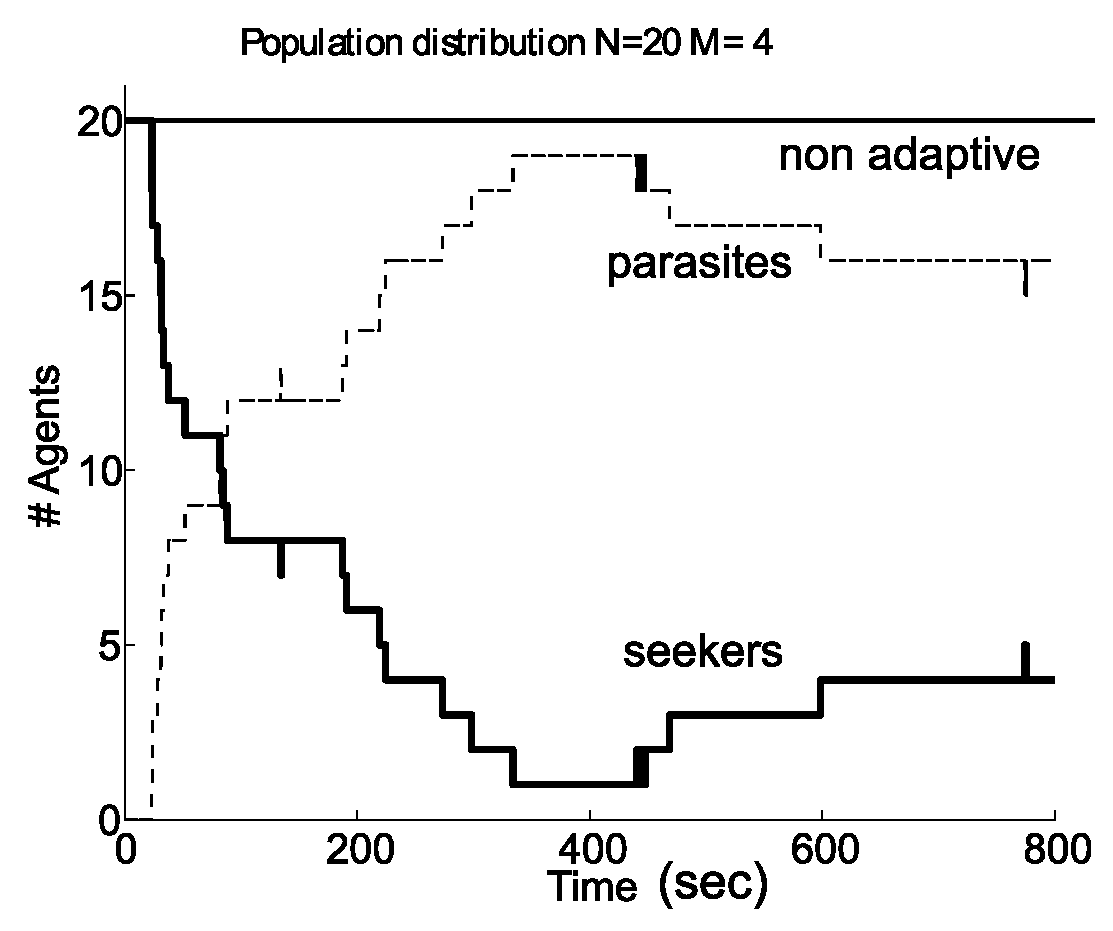
\includegraphics[width=0.4 \textwidth]{figures/socialadapt/honest/comm20TO4.eps}}
	\hspace{1pt}
      \subfigure[Honest food signal, ratio $N=20,M=16$]{
	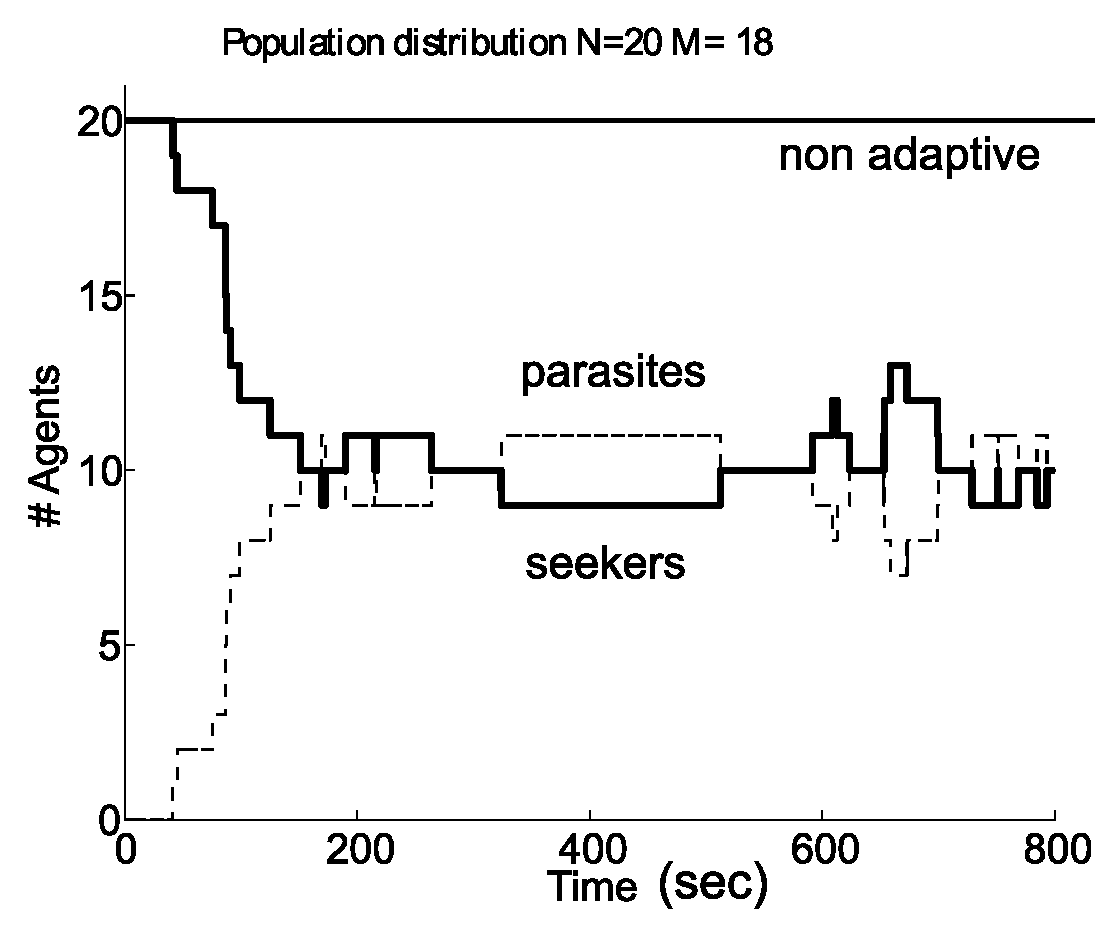
\includegraphics[width=0.4 \textwidth]{figures/socialadapt/honest/comm20TO18.eps}}
      \vspace{1pt}
      \subfigure[Dishonest food signal, ratio $N=20,M=4$, 18 cheaters]{
	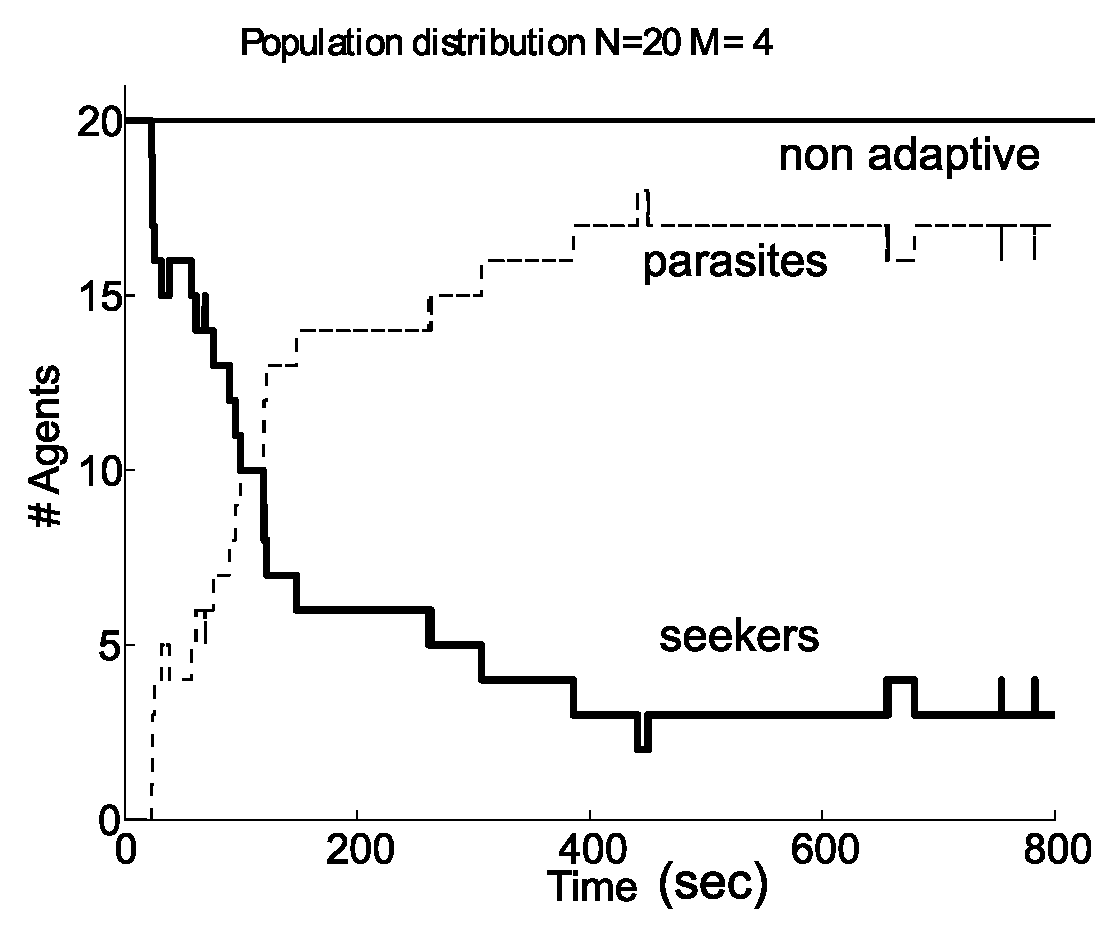
\includegraphics[width=0.4 \textwidth]{figures/socialadapt/deceptive/comm20TO4.eps}}
	\hspace{1pt}
      \subfigure[Dishonest food signal, ratio $N=20,M=16$, 18 cheaters]{
	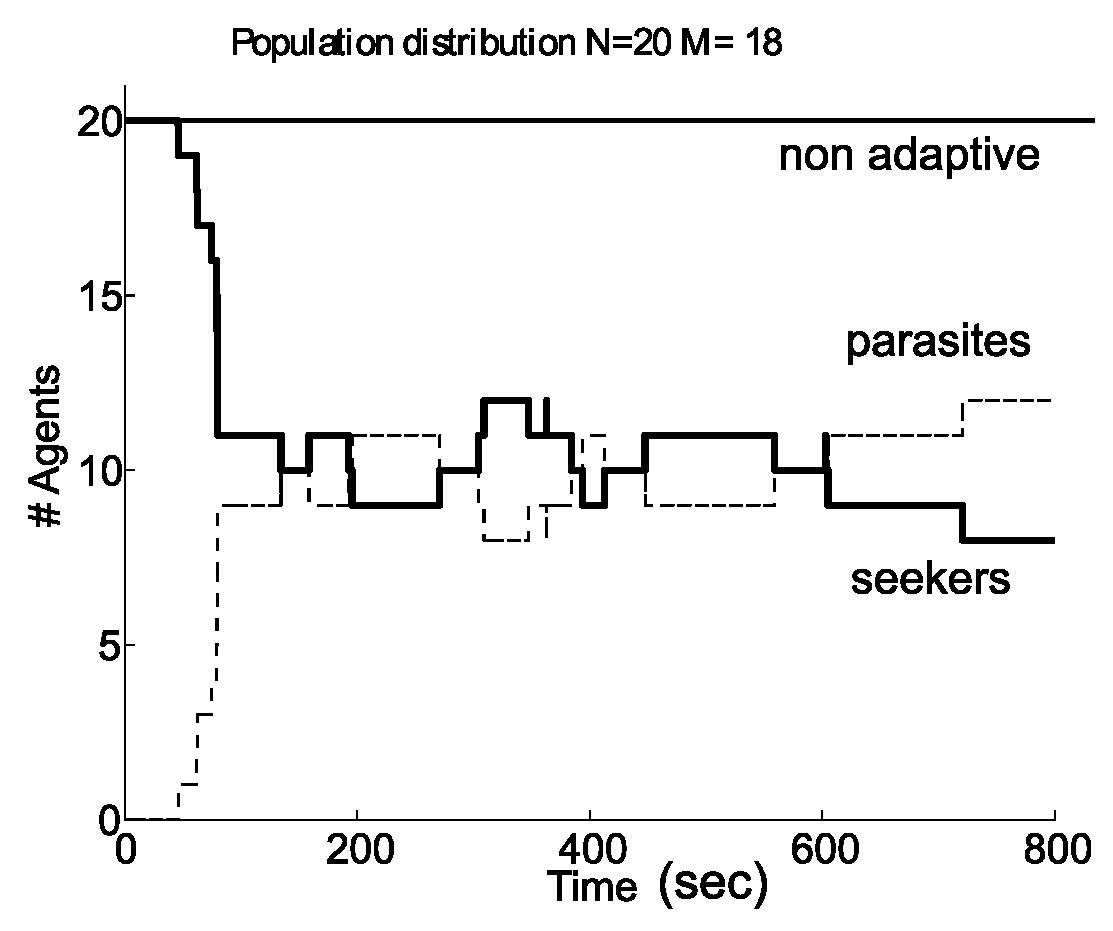
\includegraphics[width=0.4 \textwidth]{figures/socialadapt/deceptive/comm20TO18.eps}}
    \caption[Sub system formation in different conditions]{
	  Population distribution in different cases: x-axis is the simulation time expressed in seconds,
	  y-axis reports the number of seekers $n_{s}(t)$ and of parasites $n_{p}(t)$ in function of time.
	  There are 6 diagrams, and for every diagram the adaptive communication
	  strategy versus the non communicative strategy is reported. \label{fig:generalcomparison}}
  \end{center}
\end{figure}

Considering the different cases in Fig.\ref{fig:generalcomparison}, it can be said that :
\begin{itemize}
\item in non-adaptive communication: parasites are absent (also with aggressive configuration see condition \ref{eq:aggressive} ), suggesting that adaptive communication is a necessary condition for the generation of sub-systems. In all cases (a) to (f): $n_{s}(t)=20$ and $n_{p}(t)=0$ at any time.
\item parasitism is a quasi-stable condition: the numbers of seekers and thus parasites stabilise after a transitory phase. For example in case (a) population distribution reaches an equilibrium: $n_{s}(t)=5\pm 1$ and $n_{p}(t)=15\pm$ with $t>400 s$. After 800 seconds (data not shown) the population distribution oscillates around the equilibrium.
\item the population dynamic is depending on the ratio between agents $N$ and food resources $M$:
\begin{itemize}
\item with scarce resources ($M=4$) in cases (a),(c),(e) parasites are prevalent
\item with abundant resources ($M=18$) in cases (d),(f) parasites are balanced with seekers, whereas in case (b) parasites are prevalent.
\end{itemize}
\end{itemize}
Table \ref{tab:population} resumes the stabilisation property of the population for 3 main cases:
\begin{enumerate}
\item silence: agents do not use the food social signal
\item honest: agents signal the food presence honestly
\item dishonest: some agents signals the food presence dishonestly, the rest of them do not signal (like the silence case)
\end{enumerate}

There are 2 important observations to make:
\begin{enumerate}
\item the ratio of seekers over parasites ($n_{s}/n_{p}$) depends non linearly to
the ratio of agents to food sources in the silence and dishonest cases. For example in
the silence scenario (agents do not signal the food presence) $n_{s}=5,3,5$
respectively for $M=4,10,18$. Interpolation techniques suggests that the dependency
is of exponential type.
\item the ratio of seekers over parasites ($n_{s}/n_{p}$) depends proportionally to the
ratio of agents to food sources in the honest case. Number of seekers $n_{s}$ increases
accordingly with the food sources $M$ such that $n_{s}=4,8,10$ respectively for $M=4,10,18$.
\end{enumerate}

\begin{table}[htbp]
\caption[Tabular results for self organisation property]{
Table summarising self-organisation:
every element in the table is the couple $(n_{s}(T_{sim}),n_{p}(T_{sim}))$
which indicates the number of seekers and parasites when the simulation
at the end of the simulation}
\label{tab:population}
\begin{center}
\small{
\begin{tabular}{@{}c|ccc@{}}
\hline
Ratio $N/M$ & 20:4 & 20:10 & 20:18\\
\hline
Silence & $(5,15)$ & $(3,17)$ & $(5,15)$\\
\hline
Honest & $(4,16)$ & $(8,12)$ & $(10,10)$\\
\hline
Dishonest agents:2  & $(7,13)$ & $(4,16)$ & $(8,12)$\\
Dishonest agents:10 & $(5,15)$ & $(6,14)$ & $(1,19)$\\
Dishonest agents:16 & $(10,10)$ & $(3,17)$ & $(8,12)$\\
\end{tabular}
}
\end{center}
\end{table}

A possible explanation for the prevalence of the parasitic population with scarce resources is due to the space constraints of the food sources: only a few agents (in our case 9) can forage at the same time, therefore the agents learn to transport food for the others. When resources are abundant this constraint is removed therefore the parasitic strategy is no longer needed.

\subsubsection{Foraging performance and signalling strategies}
If one wants to analyse the performance of the system in consuming food,
one could measure the number of the total bites can be measured:
\begin{equation}
 F_{tot}=F_{seek}+F_{parasite} \label{social:totbites}
\end{equation}
where $F_{seek}$ is the number of total times agents touched food sources (Eq. \ref{eq:touchfood})
and $F_{parasite}$ is the number of total times that agents touched other sated agents (Eq. \ref{eq:touchagent}).
Having chosen that index, table \ref{tab:totalPerformance} shows the $F_{tot}$ 
for the different conditions and underlines the value when dishonest is superior to 
the honest strategy.
On the basis of total bites, I can state that:
\begin{itemize}
\item honest signal is better then silence when food resources are $M=4,10,18$
\item comparing the honest and the dishonest strategy:
with 10 dishonest agents the $F_{tot}$ is superior to the honest one when $M=4,10$
but not when $M=18$. With only 2 dishonest agents, $F_{tot}$ is bigger only with scarce resources.
With 16 dishonest agents, performance is superior only in the intermediate case with $M=10$ resources.
\end{itemize}
It is also obvious that the dishonest strategy pays only when resources are scarce, 
which is also intuitive and has been shown in other simulation or
behavioural experiments such as \citet{Brembs1996:CheatingPrisonerDilemma,Schwieren2010:CompetitionCheating}.
The main idea is that if everybody is cheating and is not punished, the information
in the system is no more reliable and will punish everybody indiscriminately.

\begin{table}[htbp]
\caption[Social System foraging performance]{
Table summarising the foraging performance: every value represents $F_{tot}$}
\label{tab:totalPerformance}
\begin{center}
\small{
\begin{tabular}{@{}c|ccc@{}}
\hline
Ratio $N/M$ & 20:4 & 20:10 & 20:18\\
\hline
Silence & 373 & 347 & 371\\
\hline
Honest & 385 & 358 & 376\\
\hline
Dishonest agents:2 & \underline{391} & 348 & 343\\
Dishonest agents:10 & \underline{406} & \underline{385} & 339 \\
Dishonest agents:16 & 317 & \underline{369} & 351\\
\end{tabular}
}
\end{center}
\end{table}

Another index for the system performance is the equality in the food distribution. 
It means that, if I consider the mean $\mu$ and standard deviation $\sigma$ of 
the food bites over the $N=20$ agents, the food is better distributed ideally when 
the average $\mu$ is high as well as the deviation $\sigma$ is high. 
This indicate that a good distribution is when all agents in average have a good amount of food when the deviation
is high and average is high.
But if the average is high and the deviation is low, it means that few agents have
collected a large amount of food and thus is not desirable for a sustainable society.
Table \ref{tab:foodDistribution} contains the computed values for each condition.

\begin{table}[htbp]
\caption[Social System food distribution]{Table summarising food distribution:
every element represent the couple ($\mu,\sigma$) where $\mu$ is the average of
the food bites+agents bites over the agent population, and $\sigma$ is
the standard deviation. They are calculated at the end of the simulation.
}
\label{tab:foodDistribution}
\begin{center}
\small{
\begin{tabular}{@{}c|ccc@{}}
\hline
Ratio $N/M$ & 20:4 & 20:10 & 20:18\\
\hline
Silence & $(18.65,2.16)$ & $(17.35,2.83)$ & $(18.55,4.11)$\\
\hline
Honest & $(19.25,3.00)$ & $(17.90,2.51)$ & $(18,3.27)$\\
\hline
Dishonest (2 cheaters) & $(19.55,1.85)$  & $(17.40,2.09)$   & $(17.15,3.79)$\\
Dishonest (10 cheaters) & $(20.30,2.13)$  & $(19.25,2.63)$  & $(16.95,3.41)$\\
Dishonest (18 cheaters) & $(15.85,5.34)$ & $(18.45,2.58)$  & $(17.55,2.67)$\\
\end{tabular}
}
\end{center}
\end{table}

\begin{itemize}
\item for scarce resources $M=4$ and 2 cheaters: the best distribution comes 
with honesty:  $\mu_{honest}=19.25$ and $\sigma_{honest}=3.0$.
\item for scarce resources $M=4$ and 18 cheaters: dishonest has a smaller 
average  $\mu_{dishonest}=15.85$ but a better variance $\sigma_{honest}=5.34$ 
compared to the silence and honest strategy which has respectively a $\sigma_{silence}=2.16$ 
and $\sigma_{honest}=3.00$.
\item for abundant resources the honest and silence strategies are nearly equal, 
but with silence the variance is bigger $\sigma_{silence}=4.11)\sigma_{honest}=3.27$.
\item for abundant resources and any percentage of cheaters the honest strategy 
has the larger mean $\mu_{honest}=18.3$ and a comparable variance.
\end{itemize}


\subsubsection{Adaptive vs non communicative foraging performance}
In this scenario the honest communication strategy is compared to the non 
communicative behaviour. In figure \ref{fig:foraging1} it is reported the  
the number of total bites $F_{tot}$ (see Eq. \ref{social:totbites}) on the y-axis
in function of the simulation time on the x-axis for two cases: 
adaptive and non communicative strategy when the agents use the social honest signal. 
In case (a), where resources are scarce, before the sub-systems are formed 
(before $1x10^{4}$) $F_{tot}$ is equal in both cases, but during learning and, 
furthermore when the agents organise, the adaptive case overcomes the non
 adaptive one. In case (b), where resources are abundant, $F_{tot}$ is 
equal during all the time, because a strategy to optimize the food gathering
 is not essential.

\begin{figure}[htbp]
\begin{center}
\includegraphics[scale=0.3]{figures/socialadapt/foraging1.eps}
\end{center}
\vspace*{4pt}
\caption[Foraging performance comparison]{Foraging performance comparison:
thick line is the adaptive communication with honest signalling and the
dotted line is the non-adaptive communication case with honest signalling.
\textbf{Case (a):} scarce resources adaptive communication win.
\textbf{Case (b):} abundant resources, performances are equal
\label{fig:foraging1}}
\end{figure}


\subsubsection{Honest behaviour and unlimited resources}
In this scenario the agent honestly signals the presence of food places which
always produce the $G_{food}$ potential.
For this simulation, a population of $N=20$ agents is provided with $M=4,10,18$
food places sequentially. Population dynamic is observed for a total duration
of  $T_{sim}=80000$ (time step $\triangle T=0.01 seconds$).
Figure. \ref{fig:comparison} reports the number of seekers (thick line) and
parasites (dotted line) in function of time. 
The number of seekers $n_{s}(t)$ is complementary to the number of parasites 
$n_{p}(t)$: $n_{s}(t)+n_{p}(t)=N$.
The population ratios of seeker to parasites ($r(T_{sim})$) at the end of the
 simulation for every case $M=4,10,18$ are respectively $r(T_{sim})=4/16,8/12$ and $10/10$.
\begin{itemize}
\item in non-adaptive communication: parasites are absent (also with aggressive configuration see \ref{eq:aggressive}), suggesting that adaptive communication is a necessary condition for the generation of sub-systems.
\item in adaptive communication parasitism is a quasi-stable condition. With scarce resources ($M=4$), after 600 seconds, the number of seekers (see Fig. \ref{fig:comparison} (a)) stabilises to 4. With abundant resources ($M=18$), after 600 seconds, the number of seekers (see Fig. \ref{fig:comparison} (b)) stabilises to 10. After 800 seconds (data not shown) small oscillations around the stable point occur in both cases, suggesting that the system has reached an attractor.
\item the population ratio between seekers and parasites $r(T_{sim})$ depends on the ratio between the number of robots and the number of food places $N/M$:
\begin{itemize}
\item with scarce resources ($M=4$) parasites are prevalent: $n_{p}(T_{sim})=16\pm1 > n_{s}(T_{sim})=4\pm1$.
\item with abundant resources ($M=18$) seekers and parasites are in dynamical equilibrium (oscillate around the stable point after $T_{sim}$ steps): $n_{p}(T_{sim})=10\pm1$ and $n_{s}(T_{sim})=10\pm1$.
\end{itemize}
\end{itemize}
An explanation for the prevalence of the parasitic population with scarce resources is due to the space constraints of the food sources: only a few agents (in our case 9) can forage at the same time, therefore agents "transport" food for the others. When resources are abundant this constraint is removed therefore parasitism is not essential.

\begin{figure}[ht]
  \begin{center}
      \subfigure[Case considering scarce resources: in non adaptive-communication only seekers are present (top line is constant to 20 agents), in adaptive communication sub-system formation is achieved and parasites become more than seekers after 80 seconds]{
	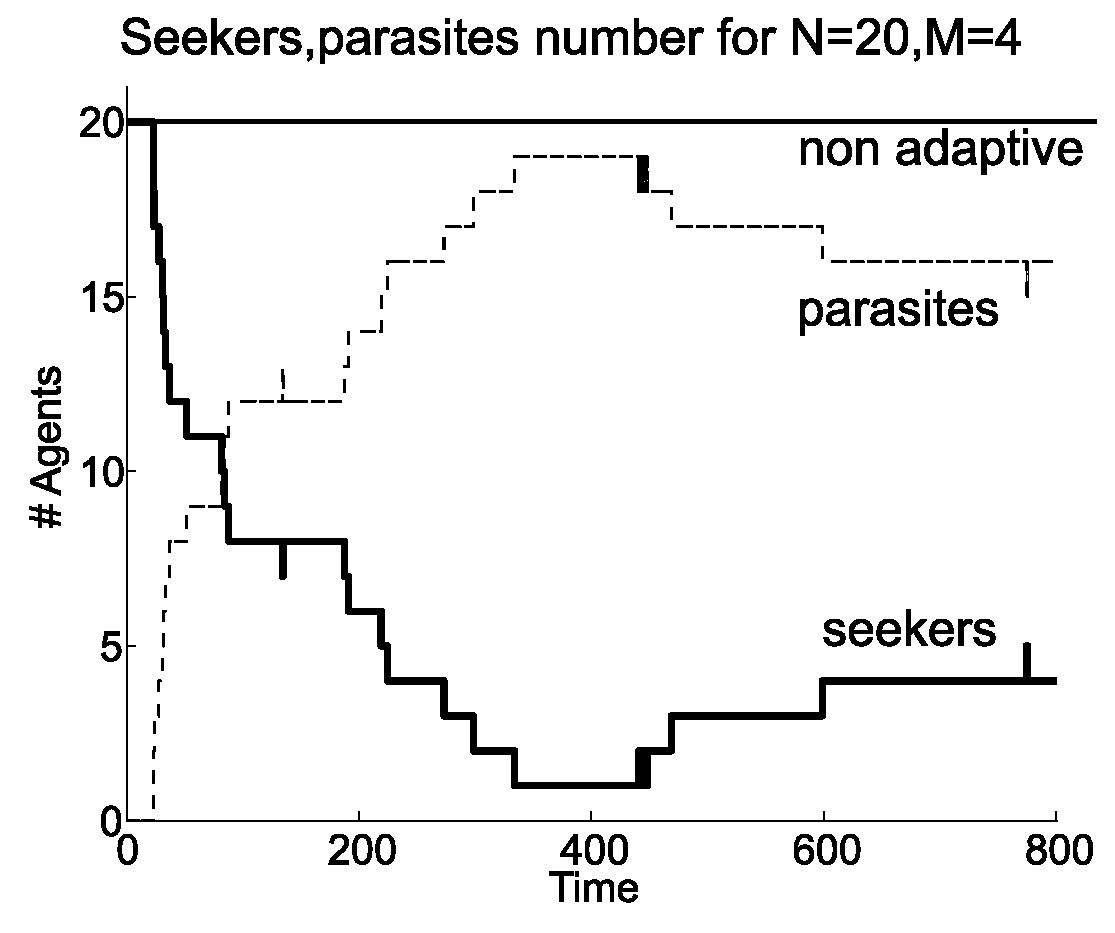
\includegraphics[width=0.4 \textwidth]{figures/socialadapt/20to4.eps}}
	\hspace{1pt}
      \subfigure[Case considering scarce resources: in non adaptive-communication only seekers are present (top line is constant to 20 agents), in adaptive communication sub-system formation is achieved and parasites are in equilibrium with seekers after 200 seconds]{
	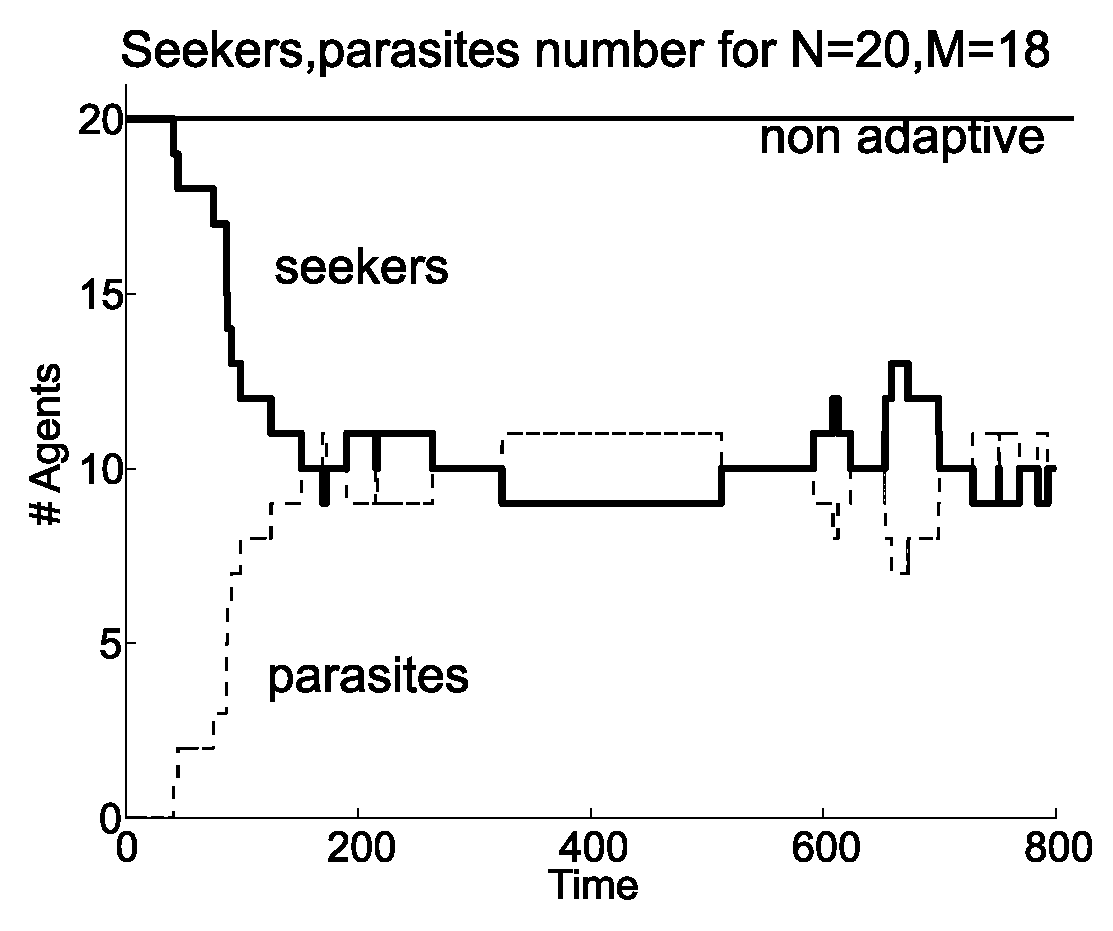
\includegraphics[width=0.4 \textwidth]{figures/socialadapt/20to18.eps}}
    \caption[Self organisation with honest behaviour and unlimited resources]{\label{fig:comparison}}
  \end{center}
\end{figure}
To analyse the performance of the system in consuming food: the number of the total bites $F_{tot}=F_{seek}+F_{parasite}$ it is considered.
$F_{seek}$ is the number of total times that agents touched food sources (Eq. \ref{eq:touchfood}) and $F_{parasite}$ is the number of total times that agents touched other sated agents (Eq. \ref{eq:touchagent}). In table \ref{tab:performance} it is reported the foraging performance (average $\pm$ range) over 100 simulations and it can be noticed that adaptive communication provides the best performance only for scarce resources and an equal performance for abundant resources.

\begin{table}[htbp]
\caption[Foraging performance with unlimited resources]{
Table summarising foraging performance over 100 simulations.
With scarce resources, performance is superior using adaptive communication,
with abundant resources performances are equal since food distribution
through parasites is not essential.}
{
\begin{tabular}{@{}cccc@{}}
\hline
Ratio $N/M$ & 20:4 & 20:18\\
\hline
Adaptive communication & $F_{tot}=396\pm2$ & $F_{tot}=319\pm2$\\
\hline
Non-adaptive communication & $F_{tot}=355\pm2$ & $F_{tot}=319\pm2$\\
\hline
\label{tab:performance}
\end{tabular}}
\end{table}

\subsubsection{Honest behaviour and limited resources}
In this scenario the agent honestly signals the presence of food which is limited in time.
For this simulation, a population of $N=20$ agents is provided with $M=4,10,18$
food places sequentially. Population dynamic is observed for a total duration
of  $T_{sim}=80000$ (time step $\triangle T=0.01 seconds$).
The population ratios of seeker to parasites ($r(T_{sim})$) at the end of
the simulation for every case $M=4,10,18$ are respectively $r(T_{sim})=5/15,8/12$
and $10/10$.
\begin{itemize}
\item in non-adaptive communication: parasites are absent (also with aggressive
configuration see \ref{eq:aggressive}), suggesting that adaptive communication
is a necessary condition for the generation of sub-systems.
\item in adaptive communication parasitism is a quasi-stable condition.
With scarce resources ($M=4$), after 600 seconds, the number of seekers
(see Fig. \ref{fig:limitedcomparison} (a)) stabilize to 5. With abundant resources ($M=18$),
after 600 seconds, the number of seekers (see Fig. \ref{fig:limitedcomparison} (b))
stabilises to 10. After 800 seconds (data not shown) small oscillations around
the stable point occur in both cases, suggesting that the system has reached an attractor.
\item the population ratio between seekers and parasites $r(T_{sim})$ depends
on the ratio between the number of robots and the number of food sources $N/M$:
\begin{itemize}
\item with scarce resources ($M=4$) parasites are prevalent:
$n_{p}(T_{sim})=15\pm1$ $>$ $n_{s}(T_{sim})=5\pm1$.
\item with abundant resources ($M=18$) seekers and parasites are in dynamical
equilibrium (oscillate around the stable point after $T_{sim}$ steps):
$n_{p}(T_{sim})=10\pm2$ and $n_{s}(T_{sim})=10\pm2$.
\end{itemize}
\end{itemize}

\begin{figure*}
\centerline{\subfigure[Case considering scarce resources: in non adaptive-communication
 only seekers are present (top line is constant to 20 agents), in adaptive communication
 sub-system formation is achieved and parasites become more than seekers after 200 seconds]{
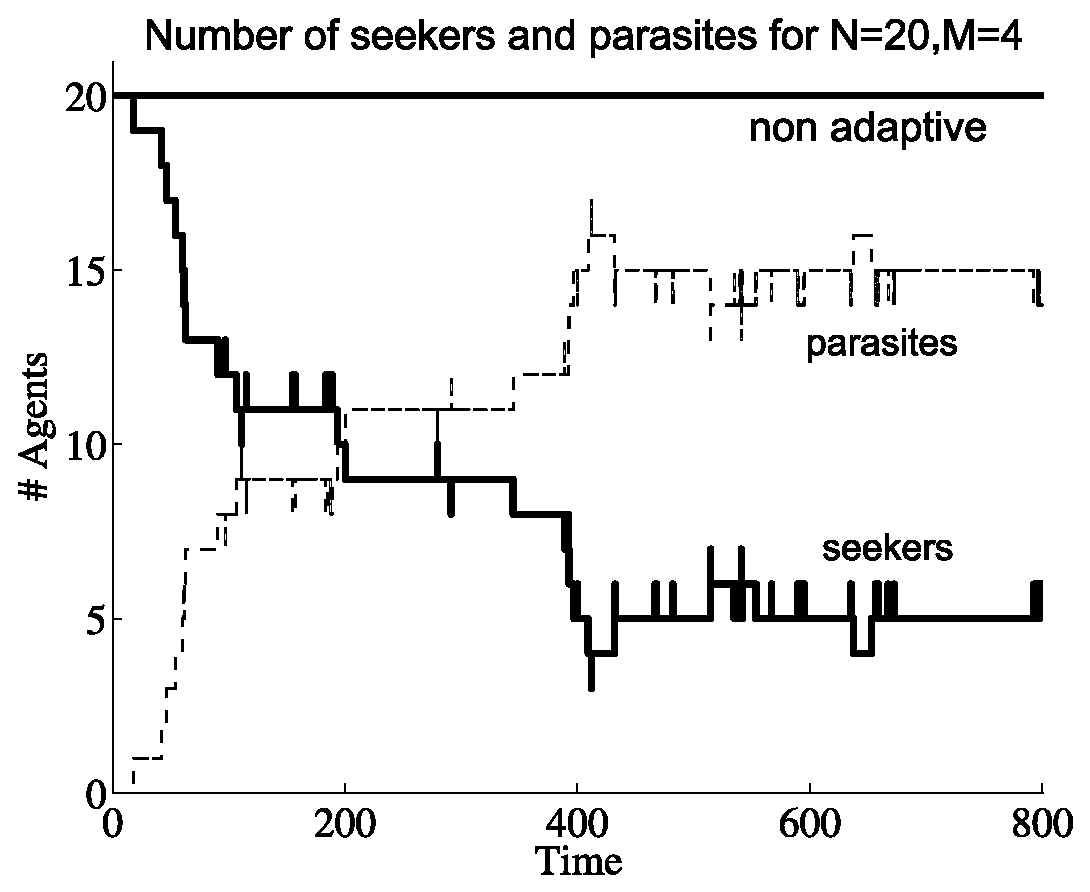
\includegraphics[width=2.4in]{figures/socialadapt/limited/20to4.eps}
\label{fig_first_case}}
\hfil
\subfigure[Case considering scarce resources: in non adaptive-communication
only seekers are present (top line is constant to 20 agents), in adaptive
communication sub-system formation is achieved and parasites are in equilibrium
with seekers after 200 seconds]{
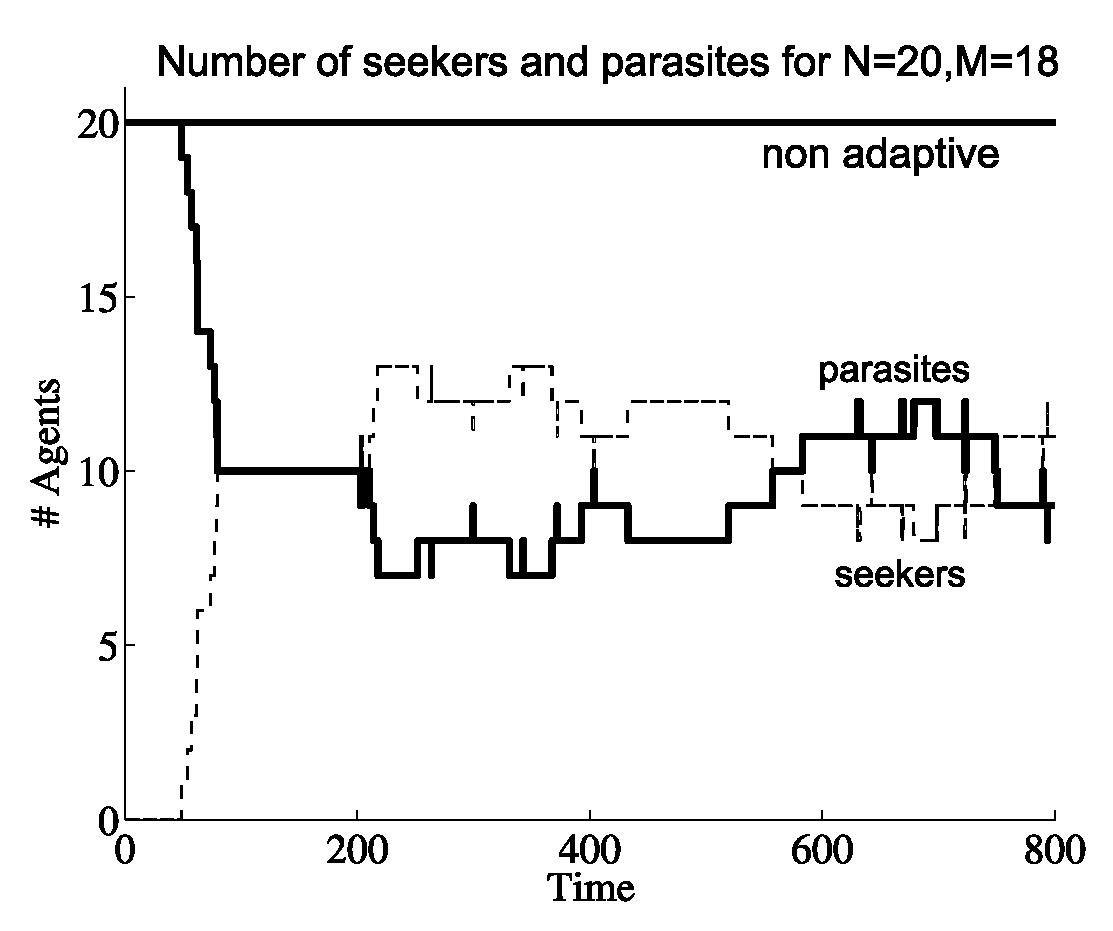
\includegraphics[width=2.4in]{figures/socialadapt/limited/20to18.eps}
\label{fig_second_case}}}
\caption[Self organisation with honest behaviour and limited resources]{\label{fig:limitedcomparison}}
\label{fig_sim}
\end{figure*}
An explanation for the prevalence of the parasitic population with scarce
resources is due to the space constraints of the food places: only few agents
 (in our case 9) can forage at the same time, therefore agents "transport"
food for the others. When resources are abundant this constraint is
removed therefore parasitism is not essential.

To analyse the performance of the system in consuming food: the number of the total
bites $F_{tot}=F_{seek}+F_{parasite}$ it is considered.
$F_{seek}$ is the number of total times that agents touched food sources
(Eq. \ref{eq:touchfood}) and $F_{parasite}$ is the number of total times that
agents touched other sated agents (Eq. \ref{eq:touchagent}).
In table \ref{tab:limitedperformance} the foraging performance
(average $\pm$ range) over 100 simulations is demonstrated and it can be noticed that adaptive
communication provide the best performance in term of food foraging for scarce
and abundant resources. Why is the performance better than the unlimited case?
Because this time the food resources are limited in time and space, so even when
 there are a lot of food resources the agents must collaborate to maximise
the food collection.

\begin{table}
%% increase table row spacing, adjust to taste
\renewcommand{\arraystretch}{1.3}
\caption[Foraging performance with limited resources]{
Table summarising foraging performance over 100 simulations.
Adaptive communication has the best performance for both scarce
and abundant resources.}
\label{tab:limitedperformance}
\begin{center}
\begin{tabular}{@{}cccc@{}}
\hline
\hline
Ratio $N/M$ & 20:4 & 20:18\\
\hline
Adaptive communication & $F_{tot}=439\pm2$ & $F_{tot}=340\pm2$\\
\hline
Non-adaptive communication & $F_{tot}=320\pm2$ & $F_{tot}=230\pm2$\\
\end{tabular}
\end{center}
\end{table}

\subsubsection{Stability analysis for changes in population}
Every self organizing system should be stable to external variations in the 
parameter space, this property is generally known as robustness to variation.
If the number of agents are changed during simulation the system reacts promptly
and stabilize to a new state. In Fig.\ref{fig:agentAdd} seekers are stabilised
in the range $4\pm1$, when 6 more agents are added at time 400,
seekers stabilize again in the range $7\pm1$

\begin{figure}[htb]
\begin{centering}
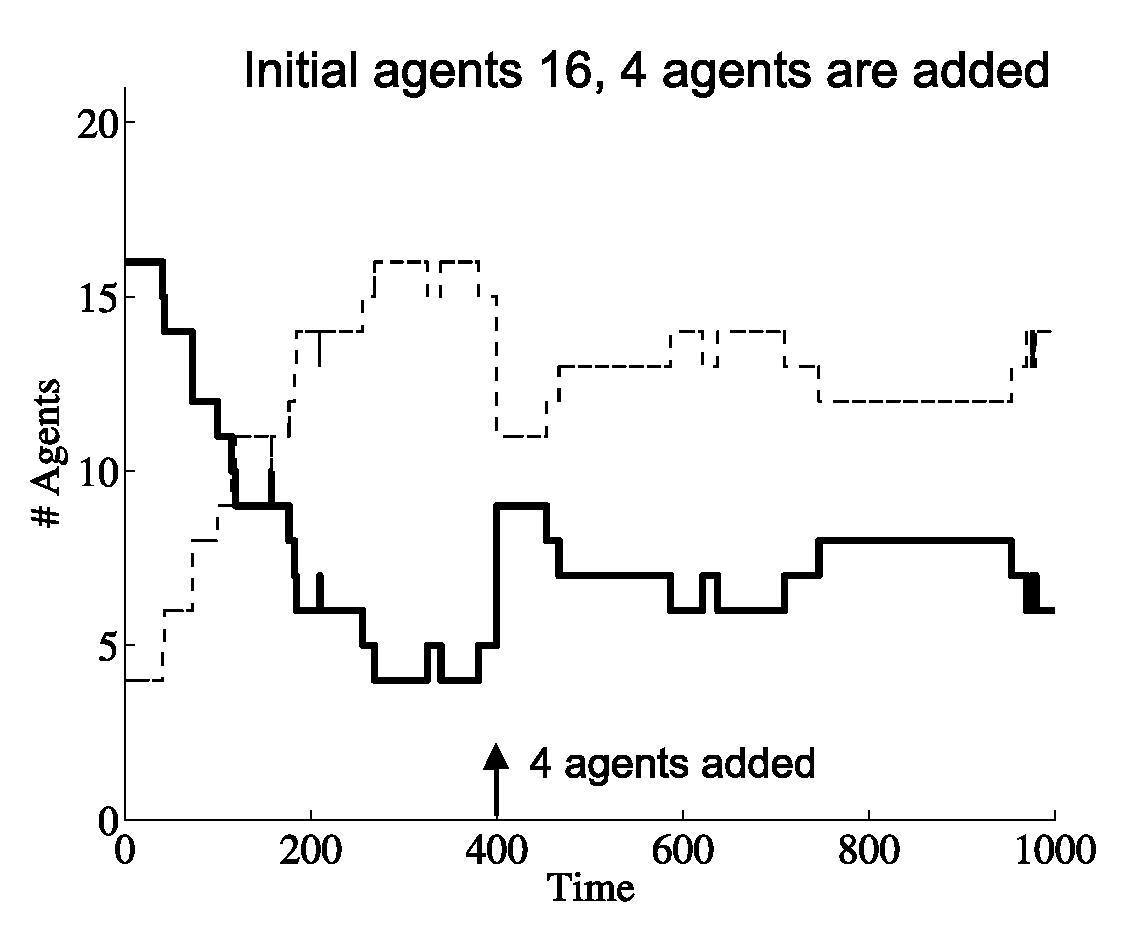
\includegraphics[width=0.6 \textwidth]{figures/socialadapt/limited/agent4more.eps}
\small{
\caption[Self organisation sensitivity to agent parameters]{
Simulation starts with 16 agents, then 4 agents are added
after 400 seconds.\label{fig:agentAdd}}
}
\end{centering}
\end{figure}

This property indicates that the system is robust to a variation in the number
of agents: the system will adjust automatically to the new equilibrium with a certain
response time.
The system is also robust to a variation in the food resources, although with 
a slower response time (not shown in the Figure).
This stability is a good feature especially for real implementation of 
social systems where disturbances from the environment are likely to occur
very often and the designer is certain that the system will be stable enough
to keep with the foraging task.


\subsection{Discussion: sub system formation in the social model}
The simulations of a social system based on pro-active learning agents has shown
very promising results.
First of all the system self-organizes by means of individual specialization 
to the environment conditions which are the number of agents and number of food resources.
Agents are based on a simple, yet effective learning mechanism called ICO which
can be extended to implement competitive behaviours.
Because internal processing is avoided, agents respond to the changes of their
environment in a timely fashion.
The system is able to generate sub-systems as Luhmann proposed by means of communication,
in absence of communication specialization is not possible.
Other embodiments for the learning controller could have been chosen, for instance
with Q-learning \citep{watkins92a} reactive agents are given a description of the
current state and have to choose the next action so as to maximise a scalar
reinforcement received after each action.
The task of the agent is to learn from indirect, delayed reward, to choose sequences of actions
that produce the greatest cumulative rewards. Reinforcement learning algorithms attempt to find
a policy that maps states of the world to the actions the agent ought to take in those states.
In economics and game theory, reinforcement learning is considered as a boundedly rational
interpretation of how equilibrium may arise. Reinforcement models for MAS suffers of 2 disadvantages:
\begin{enumerate}
\item complexity may be exponential in the number of environmental states.
\item discrete models: agents choose from a set of actions in a discretised world
\end{enumerate}
This problem is crucial in MAS: when an agent is learning the value of its actions
in the presence of other agents, it is learning in a non stationary environment.
In \citep{Qlearning-MAS} a novel exploration strategy, for
the Q-algorithm applied in a predator-prey game to obtain convergence, is introduced.
Unfortunately the cost of communication in their model is very expensive,
so they discuss only the case without communication.
Our learning rule ICO, is unsupervised and is computationally efficient (since it does not rely on states)
and inspired on the evidence that organism tends to maintain a weak homoeostasis
with the environment as demonstrated by \citet{McFarland93}.
In \citep{tan97multiagent} Q-learning is applied in a predator-prey game,
where agents cooperate in different ways. It is interesting to analyse the
communication method called sharing sensation. The model is composed of 1 hunter,
1 prey and a scouting agent. At each step, the scout sends its action and sensation
back to the hunter: the hunter relies initially on his sensation and
then on the scout's sensation. Therefore the scout can be compared in our model
 as the distal signal: hunter can see the prey at longer distances.
Performance (number of steps to capture a prey) is then compared in the 2 cases:
scouting versus no scouting. Performance is superior in the scouting case
,as well as in our model performance, it is superior when agents use both
proximal and distal signal (see table \ref{tab:performance}).
Another approach used to develop communication in MAS is in \citet{Floreano-MAS}
where a genetic-algorithm is used to evolve 1000 robots (divided in 100 colonies).
The control system used is a feed-forward neural network with 10 inputs and 3 output neurons.
The network was encoded using a genetic string of 240 bits. Synaptic weights are only
evolved and not learned and robots had a sensory-motor cycle of 50 ms.
Our controller makes use of 12 inputs (2 more) and 2 motor neurons + 1 the
$G_{satedness}$ signal, but does not use a sensory-motor cycle allowing fast responses.
Thus \citet{Floreano-MAS} makes use of genetic selection and recombination to produce
robots behaviours (communication strategies). Hence the agent system do not self organise
in classes.
Other similar works, making use of evolved recurrent neural networks
(RNNs \nomenclature{RNN}{Recurrent Neural Networks})
are reported in \citet{EmergenceCommMas} and \citet{OriginsComm}. In \citet{OriginsComm}
a population of agents evolved for the ability to solve a collective navigation problem
develop individual and social/communication skills. A particular evolved behaviour
resembles our system differentiation: ``a differentiation of the modalities with
which communication is regulated (... e.g. specialised asymmetrical interaction
forms in which one robot acts as a speaker and one robot acts as an hearer)''.
In \citep{EmergenceCommMas} the evolutionary adaptivity of RNNs to
varying environmental conditions, such as the number of interacting robots is studied.
In my model the system specializes in a group that gets the food and distributes it (seekers) and
the other one (parasites) collects it.
The communication strategy was robust only for small changes. In our model,
agents adapt continuously to the environment, they self-organise efficiently
with varying robot number $N$ and varying $M$ food sources.
Moreover the system converges to a quasi-stable state thanks to the stability
provided by the learning rule.
The system performance in terms of food foraging behaviour was analysed for 
a honest and dishonest signalling strategy both in terms of food distribution
and in terms of total energy acquired.
This study can be used to predict the performance of a social robotic system in
a real test case so that the designer can choose the parameters according to the
desired performance.
In the following sections, I will introduce input measures that quantify the
agent performance and information selection as suggested by Luhmann. 







\section{An input based information measure for adaptive controllers}
\label{Chapter5:Max Corr Input}

This Section describes the development of an information measure
to assess the learning performance of the, previously described, learning agents
in the social system.

Therefore the main purpose of this Section is to introduce a couple of correlation 
based performance measures which are computed at the sensory inputs of the agent.
The first measure is called \textbf{maxcorr}, is very simple and
can be computed in real time without any probability estimation.
The \textbf{maxcorr} measure can then be normalised by using a logarithmic approach
to express the learning performance in terms of bits and thus is called \textbf{AI measure} .
The simplicity of the AI measure derives from the dependency on the
representation used by the controller/agent, but it has the disadvantage of
not being general, as described in the discussion.

\subsection{Introduction to the maxcorr input measure}
This section describes an information measure suitable for closed loop
controllers that makes use of temporal unsupervised learning. It can be applied
for example to ICO/ISO learning, differential and temporal Hebbian learning.
This information measure estimates how much the agent/controller has learnt
and is directly correlated to the weight change of the learning rule used.
The measure is based on the agent's perspective (at the input side) rather
than at output side as previous approaches. Looking at the output is equivalent
 to analysing behaviour and has a disadvantage: agents adapt to the complexity
of the environment thus even a simple reactive agent has increasing complex
behaviour in an increasingly complex environment \citep{NolfiInteraction}.
As I argued before in the previous Section \ref{Introduction:InfoTheoryClosedLoop}, 
organisms perform input control because
neural activity (motor output) generates other neural activity (sensory input) and 
so it is clear that an input measure can capture the performance of any agent, especially
 the one that are based on ICO/ISO controllers which performs input correlation.
Input                                                                                                                                                                                                                                                                                                                                                                                                                                                                                                                                                                                                                                                                                                                                                                                                               control is a closed loop property and is agent centric, whereas output control is 
observer centric. 
To my best knowledge, this is the first approach for the closed loop case,
which is not based on the traditional concept of Shannon's entropy.
In this model agents are learning to avoid obstacles and each other using a proximal signal
(touch sensor as pain) and a predictive signal (vision). An information
measure is computed on these inputs to verify if the agents are learning.
Firstly the author introduces the information measure based on the cross correlation
of the agent inputs, then he applies the measure to two types of agent controllers (a complex and a simplified model)
for an avoidance task with multiple agents.
Finally the measure is computed on the social setting described in section \ref{Chapter4:Social adaptation}.

\subsection{Methods: controller assumptions}
The following assumptions were made for the development of the measure:
\begin{itemize}
\item the controller is a MIMO (multi input multi output) or MISO (multi input single output)
\item input signals can be analog or digital
\end{itemize}

The closed loop measure is based on the cross correlation to be applied to the
input signals (minimum is 2) of the adaptive controller.
Cross correlation of two real analog signals $x(t),y(t)$ of a real variable $t$
(in our case time), denoted as $corr(x,y)$ is defined by:
\begin{equation}
corr(x,y)=\int_{-\infty}^\infty x(\tau)\,y(t+\tau)d\tau.
\end{equation}
Cross correlation for realisable devices (software or hardware implementations)
must be computed in finite time, that means computing the cross correlation
in a limited time window $T<\infty$:
\begin{equation}
corr(x,y)=\int_{t}^{t+T} x(\tau)\,y(t+\tau)d\tau.
\end{equation}
Cross correlation for digital signals (sampled analog signals) as two discrete
time series $x_{n},y_{n}$ with $n=1,..,N$ is defined as:
 \begin{eqnarray}
 R_{xy}(m)=\sum_{n=0}^{N-m-1}x_{n+m}y_{n} & m \geq 0 \\
 R_{yx}(-m)=0 & m <0\\
 c_{xy}(m)=R_{xy}(m-N) & m=1,2,...,2N-1\label{eq:xcorrdigital}
\end{eqnarray}

The cross correlation give us a measure of the linear synchronisation between x and y.
Its absolute values range from zero (no synchronisation) to 1 (maximum synchronisation)
and it is symmetric: $c_{xy}(m)=c_{yx}(m)$. Peaks in the cross correlation determine
the phase delay between signals (for other cross-correlation variation see \ref{Appendix:crosscorr}).

The next section describes a complex model for an avoiding robot using the ICO
learning rule.

\subsection{Methods: complex model configuration}
The simulation model is composed of a 2 dimensional world bounded by walls
as described before in Chapter \ref{WorldModelSim}.
The agents are indexed by their position as $a_{j}(t)$, where $a_{j}$
has 2 components (x,y coordinates indexed by $a_{j,x}$ and $a_{j,y}$),
with $j=1,..,N$. Agents move with a differential drive system (two wheels).

In this configuration the agent has only an avoidance behaviour:
\begin{itemize}
\item left and right reflexes makes him retract when both synapses are active
\item left and right distals are being used later on when the agent has learned
the association of distal to reflexes.
\end{itemize}

Agents and walls are obstacles. Agents produce obstacle signals.
Every agent $a_{j}(t)$ has a potential field associated (see Eq.\ref{eq:circle}):
\begin{equation}
Gavoid_{j}(t)=G(x-a_{j,x}(t),y-a_{j,y}(t)).
\end{equation}
that is sensed by the corresponding inputs of other agents $a_{k}(t)$
(with $k\neq j$) labelled as $avoid_{left,right}$. Walls
don't produce $G_{avoid}$, so that agents sense them using proximal signals that are
generated by collisions: when 2 distinct agents $j$ and $l$ collide at time $t_{0}$, such
that $||a_{j}(t)-a_{l}(t)||_{2}<D$ ($D$ is the radius of the
agent) an impulse is produced an impulse is produced at $avoid_{l,r}$.
\begin{figure}[htb]
\begin{center}
\includegraphics[scale=0.45]{figures/infomeasure/avoidance.eps}
\end{center}
\vspace*{4pt}
\small{
\caption[Avoidance ICO behaviour]{
Avoidance network: ICO left and right are two neurons implementing the
ICO learning rule, their output is a sigmoid and is connected (after
normalisation into $[v_{min},v_{max}]$) to the motor speed commands.
Grey triangles represent distal inputs, while white triangles represent
proximal inputs. The learned synaptic weights are associated to the distal
synapses (thick lines) while the fixed are associated to the proximal synapses
(dotted lines). To produce a retraction behaviour left and right weights
must be different such that
$W_{predict,L}>W_{predict,R}$ and $W_{reflex,L}>W_{reflex,R}$, if
$W_{predict,L}=W_{predict,R}$ and $W_{reflex,L}=W_{reflex,R}$ robot
will just go back without turning.\label{fig:inputcorr:avoidance}}}
\end{figure}
The agent's controller, (shown in Fig. \ref{fig:inputcorr:avoidance}) is composed of:
\begin{itemize}
\item two input synapses: left and right with one reflex and one distal signal per synapse.
\item two ICO neurons: left and right cross connected as left synapse with right motor and right synapse to the left motor.
\item two output motors: respectively for the left and right ICO neuron connected to the left and right motor speed.
\end{itemize}

Every ICO neuron (left and right) has 2 corresponding reflexes
(left, right short range sensors) connected:
\begin{eqnarray}
x_{0,l}(t)=avoid_{prox,r}(t) & x_{0,r}(t)=avoid_{prox,l}(t)
\end{eqnarray}
and 2 corresponding predictive signals (left, right long range sensors) connected:
\begin{eqnarray}
x_{1,l}(t)=avoid_{dist,r,d_{o}}(t) & x_{1,r}(t)=avoid_{dist,l,d_{o}}(t).
\end{eqnarray}

The neural controller for the avoidance behaviour is shown in
Fig. \ref{fig:avoidance} \citep{Stamm2006}, every ICO neuron (left and right)
computes the following operations:

\begin{eqnarray}
ICO_{L}(t)&=B-h \ast x_{0,r} \cdot W_{reflexL}-h \ast x_{1,r}\cdot W_{predictL}\\ \nonumber
	  &+W_{selfL}\cdot ICO_{L}(t-1) + W_{L2R}\cdot ICO_{R}(t) \label{eq:input:ICO:L1} \\ 
ICO_{R}(t)&=B-h \ast x_{0,l}\cdot W_{reflexR}-h \ast x_{1,l}\cdot W_{predictR}\\ \nonumber
	  &+W_{selfR}\cdot ICO_{R}(t-1) + W_{R2}\cdot ICO_{L}(t)  \label{eq:input:ICO:R1}
\end{eqnarray}

The parameters used for the weights, the bias and the recurrent connections are
reported in the Appendix sections \ref{Appendix:HysteresysValue},\ref{Appendix:simulation}.
The recurrent connections between the left and right ICO neuron, are necessary
to implement a push-pull behaviour so that when the robot synchronously activates
both the left and the right input, only one ICO neuron will dominate thus evoking
a turn-back response. 
Connections between input synapses and ICO neurons (motor neurons) are
negative to evoke a retraction. 
The motor output is calculated with a sigmoid activation function on the ICO neuron
membrane as follow:

\begin{eqnarray}
V_{L}&=& \frac{1}{1+e^{-ICO_{L}}}\\
V_{R}&=& \frac{1}{1+e^{-ICO_{R}}}
\end{eqnarray}

The weight update learning rule is calculated for the weights:

\begin{eqnarray}
\frac{\partial W_{predict,L}}{\partial t}&=& \mu \cdot x_{1,l} \frac{\partial x_{0,l}}{\partial t} \label{eq:maxcorr:wleft}\\
\frac{\partial W_{predict,R}}{\partial t}&=& \mu \cdot x_{1,r} \frac{\partial x_{0,r}}{\partial t} \label{eq:maxcorr:wright}
\end{eqnarray}


\subsection{Methods: cross correlation and ICO learning}
Cross correlations are computed for the left and right synapse at fixed non
overlapped time windows $\triangle T$ expressed in seconds.
Considering Eq. \ref{eq:xcorrdigital} $N_{s}=\triangle T/\delta t$ is the number
 of samples in a time window of $\triangle T$ with a $\delta t$ as sampling time.
Left and right cross correlations are computed for every non overlapping time window $k=1,2,...$
\begin{eqnarray}
xcorr_{left}(k)=corr(H(x_{1,l}),H(x_{0,l}))=corr(u_{1,l},u_{0,l})\\
xcorr_{right}(k)=corr(H(x_{1,r}),H(x_{0,r}))=corr(u_{1,r},u_{0,r})
\end{eqnarray}
where $k$ is the index of the time window where the cross correlation was computed,
$H$ is a high pass filter that removes the constant component (generally referred as $DC$)
from the cross correlation diagram. Removing the $DC$ bias is necessary for the application
of statistical measures (see Appendix \ref{Appendix:crosscorr}).
In our model the high pass filter $H$ because the inputs of my artificial agents 
are receiving only discrete events, so essentially impulses with a 0 bias as in figure \ref{fig:ico}.
For every time window $k$, I computed the maximum $max$, energy $E$,power $P$ of the
left $xcorr_{left}(m,k)$ and right $xcorr_{right}(m,k)$ cross correlation plus the average of
the weight change for left and right $W_{predict,L},W_{predict,R}$.
\begin{eqnarray}
M(xcorr_{left}(k))=& \max\limits_{m}(xcorr_{left}(m,k)) \label{eq.maxcorr:mleft}\\
M(xcorr_{right}(k))=& \max\limits_{m}(xcorr_{right}(m,k)) \label{eq.maxcorr:mright}\\
E(xcorr_{left}(k))=& \sum\limits_{m} xcorr_{left}(m,k)^2  \\ 
E(xcorr_{right}(k))=& \sum\limits_{m} xcorr_{right}(m,k)^2 \\ 
P(xcorr_{left}(k))=& \frac{\sum\limits_{m} xcorr_{left}(m,k)^2}{N} \\
P(xcorr_{right}(k))=& \frac{\sum\limits_{m} xcorr_{right}(m,k)^2}{N} \\
Avg(W_{predict,left},k)=&\frac{\sum\limits_{m} W_{predict,left}(m+k N_{s})}{N_{s}} \\
Avg(W_{predict,right},k)=& \frac{\sum\limits_{m} W_{predict,right}(m+k N_{s})}{N_{s}} \\ 
\end{eqnarray}
The reason why I have computed this values for the left and right synapse is that
these weights develop independently from each other as in Eq. \ref{eq:maxcorr:wleft},\ref{eq:maxcorr:wright}.
Since energy and power are related measures only energy is computed (see Appendix \ref{app:energy}).
The average of the weight change for the left and right distal synapses is computed
 to validate the information measure for the result section.

\subsection{Methods: a simplified model}
The agent controller can be over simplified by using only one weight and thus one
ICO controller for the avoidance behaviour.
The difference between the left and right far antennas provides $x_{1}$ and the
difference between the left and right near short antennas provides $x_0$.
The band pass filters in Fig.\ref{maxcorr:methods:ico1} generate $u_{0},u_{1}$
that are damped waves if $x_0,x_1$ are delta pulses.
The transfer function of the band pass filter is specified in the Laplace-domain as:
\begin{eqnarray}
h(t)& &\leftrightarrow H(s) =\frac{1}{(s+p)(s+p*)}\\
h(t)&=&\frac{1}{b}e^{at}sin(bt)\\
a &=&-\pi \frac{f}{q}\\
b &=&\sqrt{(2\pi f)^2 -a^{2}}
\end{eqnarray}
where $p*$ represents the complex conjugate of the pole $p = a + ib$, $f$ is the
oscillation frequency and $q$ is the quality factor of the filter.
ICO correlates the predictive signal $u_{1}$ with the reflexive signal $u_{0}$
according to the formula:
\begin{equation}
 \frac{d\omega_1}{dt}=\mu \cdot u_1 \cdot \frac{du_0}{dt}
\end{equation}
where $\omega_1$ functions now as the weights of the more complex model in Eq. \ref{eq:maxcorr:wleft},\ref{eq:maxcorr:wright}.
Then the output $z$ of the controller is used to control the steering angle of
the robot such that an obstacle on the left $u_0>0$ will produce an anticlockwise turn,
whereas an obstacle on the right $u_0<0$ will produce a clockwise turn.
The controller learns to avoid the error signal $u_{0}$ using the predictive
signal $u_{1}$. Fig.\ref{maxcorr:methods:ico1}(A) illustrates how the learning
is achieved and (B) describes how the agents interact with the world.
A purely reactive agent has only a reflexive behaviour via $u_0$ and will never
learn to avoid the loop error signal $u_{0}$: it will touch the obstacle and
produce a trajectory like (1). When the agent starts to learn ($\omega_{1}>0$)
it will use the $u_{1}$ to prevent $u_0$, thus avoiding the obstacle before touching
it like the trajectory in (2).
Figure \ref{maxcorr:methods:ico1}(C) shows how the reflex signal is shifted forward
in time and reduced in amplitude due to the anticipatory motor reaction of the controller.
\begin{figure}[!htbp]
\begin{center}
%\framebox[4.0in]{$\;$}Schematic1
%\fbox{\rule[-.5cm]{0cm}{4cm} \includegraphics[scale=0.6]{Schematic1} \rule[-.5cm]{4cm}{0cm}}
\includegraphics[width=0.6 \textwidth]{figures/infomeasure/simple/simplemodel.eps}
\end{center}
\caption[Simplified control model]{A) Schematic diagram of the closed-loop learning
 system with inputs $x_0$ and $x_1$, synaptic weights $\omega_0$ and $\omega_1$ and
 motor output $z$. $P_0$ and $P_1$ are the transfer functions of the reflexive and
 the predictive pathway. BP block is a 2 pole band pass filter. B) Agent setup with
 short range antennas (reflexive inputs, $x_0$) and long range antennas (predictive inputs, $x_1$).
The agent is learning to avoid obstacles and walls using its short and long range antennas.
The motor reaction will reduce the intensity of the painful reflex $x_0$ as well as
 delay its occurrence. C) Schematic diagram of the input correlation learning rule
 and the signal structure \citep{Porr2006ICO}. The $u_0$ and $u_1$ are respectively
 the difference between the filtered values of the left and right antennas of
the agent. During learning the $u_0$ peak will be shifted in time and reduced
 in amplitude.} \label{maxcorr:methods:ico1}
\end{figure}

\subsection{Methods: anticipatory information}
Within the simplified model, the equations in \ref{eq.maxcorr:mleft} and \ref{eq.maxcorr:mright}
collapse in a unique value which is defined as $cc(t)$ as in Eq. \ref{eq:maxcorr:cc}.
Intuitively the information measure grows when the agent is using anticipatory information
and is zero when the agent is not able to predict its reflex.
Before learning the predictive signal $u_1$ is followed always by the reflex signal $u_0$
with the same amplitude, while after learning the amplitude of $u_0$ is likely reduced.
An ideal learner will be able to reduce totally the reflex $u_0$ to 0.
One will also notice that generally, after learning, the reflex $u_0$ will not only
be reduced but also delayed in time.

\begin{figure}[htbp]
\begin{center}
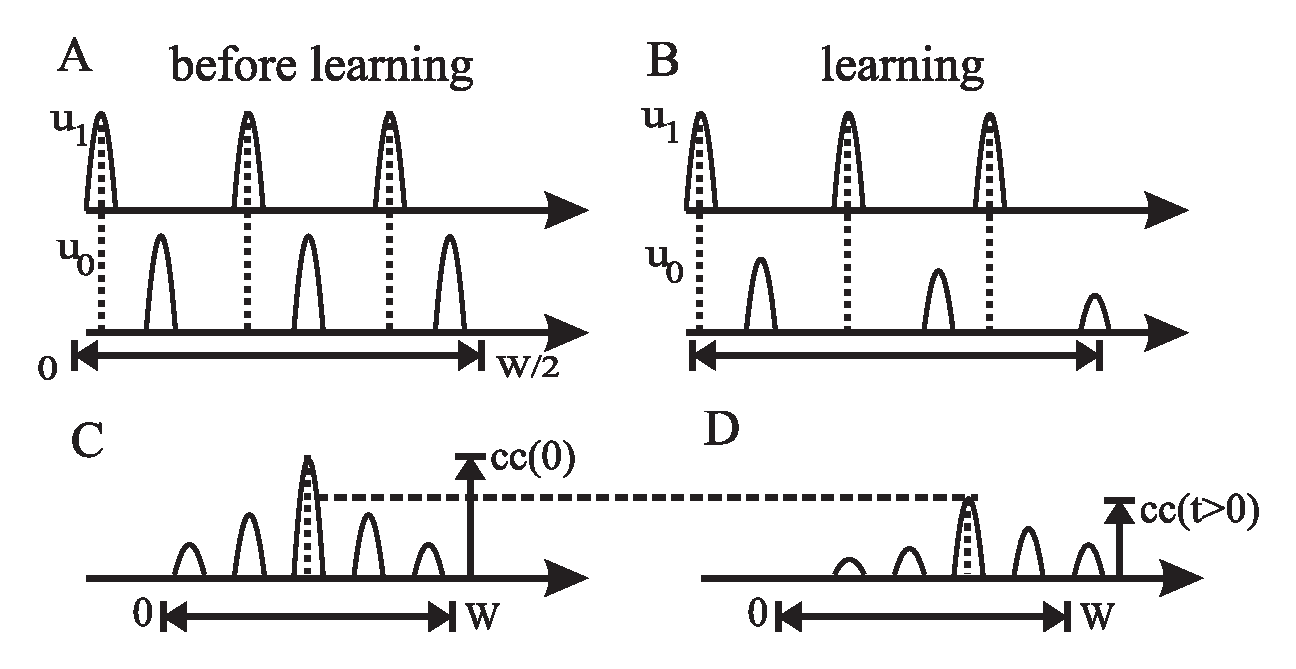
\includegraphics[width=0.6 \textwidth]{figures/infomeasure/simple/temporalsignal.eps}
\end{center}
\begin{small}
\caption[Temporal signal development during learning]{A) Illustration of the signals $u_1,u_0$
of a non learning agent. The peaks are periodic but off phase and with same amplitude.
B) Same time diagram for a learning agent. C) Cross correlation of $u_1$ and $u_0$ for the non learning case.
D) Cross correlation of $u_1$ and $u_0$ for the learning case.}
\label{methods:xcorr}
\end{small}
\end{figure}

Fig.\ref{methods:xcorr} shows a typical temporal diagram of events for a non
learning agent A and for a learning one B.
If one takes the cross correlation between the $u_1$ and $u_0$ for both cases,
it is possible to understand by the cross correlation which agent is learning and
 which one is not. For instance the non learning agent has a cross correlation
that is not shifted in time and reduced in amplitude like in Fig.\ref{methods:xcorr}(C),
while a learning agent has a cross correlation that is shifted in time and reduced
in amplitude like in Fig.\ref{methods:xcorr}(D).
My purpose is now to quantify this performance by using an information based measure
in terms of information bits.
Therefore a normalised version of $cc(t)$,$AI$ is computed in 2 steps:
\begin{align}
cc(t)=max (\sum_{\tau=-\frac{W}{2}}^{\tau=\frac{W}{2}} u_{1}(t)\cdot u_0(t+\tau)) \label{eq:maxcorr:cc}\\
AI(t)=-log_{2}(\frac{cc(t)}{cc(0)})\\
0 \leq \frac{cc(t)}{cc(0)} \leq 1
\end{align}
$cc(t)$ is the maximum of the cross correlation between the error signal and
the predictive signal in the time window $W$ that must be sufficiently large
to take at least a pairing of $u_1$ with $u_0$ when learning is off. $cc(0)$
is the maximum of the cross correlation computed when the agent is not learning,
whereas $AI(t)$ takes the ratio between the current and the initial cross correlation,
thus the argument of the logarithm will range from 0 to 1 because the correlations
following the first one can at least be equal to the first one.
When learning is off, the agent's predictive signal precedes the reflex signal whose
amplitude is not reduced hence $AI\simeq 0$, when learning is on, the agent learns
to reduce the error $u_{0}$, using an earlier motor reaction elicited by $u_{1}$,
thus the $AI \rightarrow \infty$ in the ideal case of perfect learning.
In terms of information bit, a reduction of $cc(t)$ by half can be interpreted
as an improvement of 1 bit as discussed in the results section.
In terms of information, if the agent is learning continuously the number of bits of
the $AI$ will increase in time until the agent has completely avoided the reflex.
In the next section I go back to the complex model and compute the cross correlation
and energy for the left and right synapses.
After that I will perform a benchmark of $AI$ for a the simplified model.
Both measures are taken in a multi agent scenario to see the effects of 
multiple learning agents.
I then compute the $AI$ for the simplified model in the social system and
draw some conclusions.

\subsection{Results: complex model results}
Simulations with the complex model were executed with an increasing number of agents in a rectangular
bi-dimensional world with obstacles. 
The software used to simulate the agents is Enki \footnote{http://home.gna.org/enki/}
an open source simulator for multiple robots interacting on a flat surface.
The simulator implements collisions, physics support (like slip, friction etc..)
and features 4 realistic robots.
For our simulations I used a group of Alice robots and setup the experiment as follow:
\begin{itemize}
\item $N=2$ agents and  $M=2$ obstacles
\item $N=4$ agents and $M=2$ obstacles
\item $N=4$ agents and $M=2$ obstacles, and an introduction of an agent
\end{itemize}
Agents for every case are numbered from $0$ to $N-1$.
The world's area $A_{world}$ is proportional of a factor $K$ to the sum of the agent's area:
\begin{equation}
 A_{world}=K_{a} \cdot (\sum_{i=1}^{N} A_{agent} )+ K_{o} \cdot (\sum_{i=1}^{M} A_{obstacle} )
\end{equation}
where  $A_{world}$,$A_{agent}$,$A_{obstacle}$ are respectively the area of the world,
the area of the agent and the area of the obstacle.
This normalisation technique is necessary to provide approximately the same amount 
of sensory events when the area get more crowded.
Intuitively speaking, if I keep the same area and add an increasing amount of agents
there will be a proliferation of collision and thus reflexes as well as predictor
events and thus comparison of the measures will not be reliable.
Simulation time for every setup was set to $T_{max}=600000$ steps,
$\triangle T=600 $, with sampling time $\delta t=0.01$ seconds.
Learning is switched on $\mu >0$ for $t> \triangle T=600$:
the cross correlation of the first time window is
computed when agents are only using reflexes (reactive agents).
If I compute the measure for two purely reactive agents as in Fig. \ref{entropy:reactive},
I can see that the values are constant for the left and right synapse: the agent is not learning
anything about the causal relations of distal and proximal signal.
This is because the $u1$ event is followed always by a $u0$
with the same amplitude and thus $xcorr$ amplitude is steady as described in the 
simplified model of Figure \ref{methods:xcorr}(A,C).

\begin{figure}[ht]
  \begin{center}
    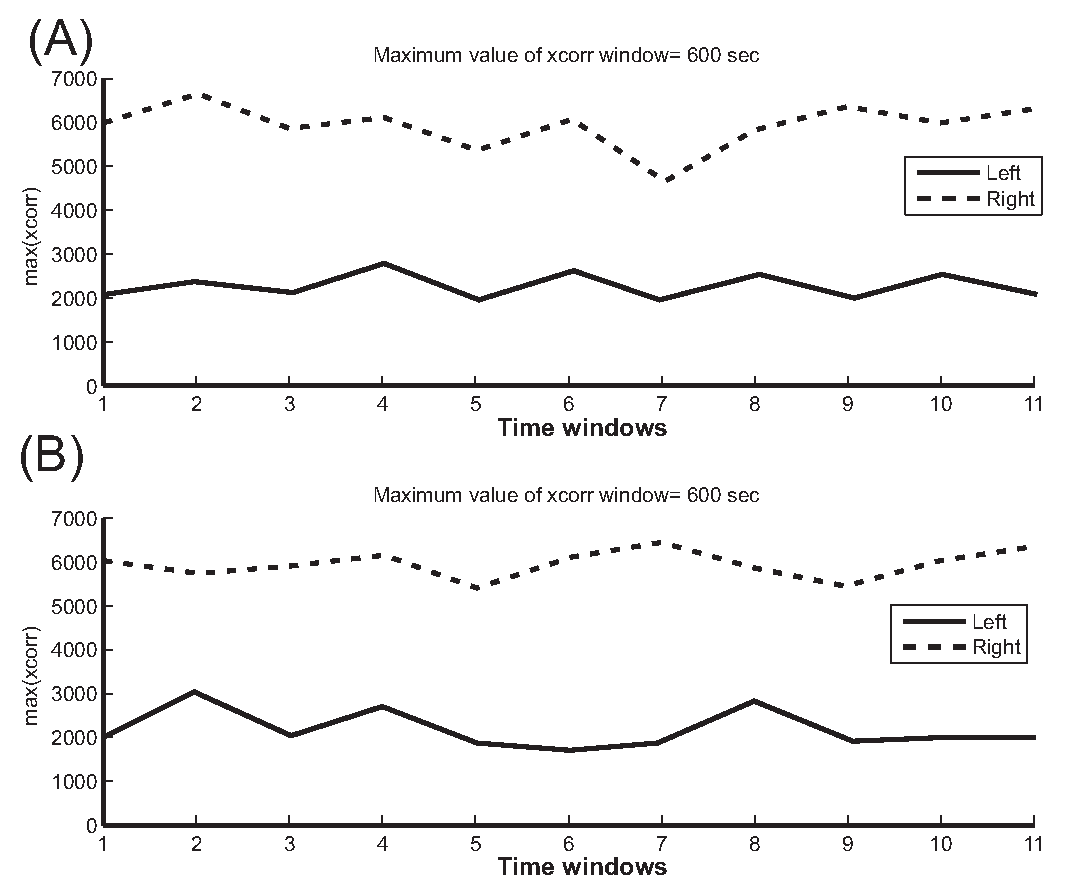
\includegraphics[scale=0.6]{figures/infomeasure/maxcorr_nolearn.eps}
    \caption[Max correlation for non learning agents]{
	     Two agents are moving in the environment without learning $\mu=0$.
	     The $M(xcorr_{left}(k)),M(xcorr_{right}(k))$ are computed for each reactive agent, A and B.
	     The measure is constant: agents are not learning anything from
	      the environment. \label{entropy:reactive}}
  \end{center}
\end{figure}
Another important property to notice in Fig. \ref{entropy:reactive} is the difference
in the offset between the $M(xcorr_{left}(k))$ left maximum cross correlation and
the $M(xcorr_{right}(k))$ right maximum cross correlation.
This is due to the initial bias of the avoiding behaviour for the agent, because 
$W_{predict,L}>W_{predict,R}$ and thus the agent tends to turn on the left each
time an obstacle is encountered.

\paragraph{Experiment with 2 agents and 2 obstacles}
Fig.\ref{fig:N2M2} shows the measures for $N=2$ learning agents and $M=2$ obstacles.
\begin{itemize}
 \item Fig.\ref{fig:N2M2}(a) contains the $M(xcorr_{left}(k))$, $M(xcorr_{right}(k))$ in the upper panel
and the $Avg(W_{predict,left},k)$, $W_{predict,right},k)$ in the lower panel for the first agent.
 \item Fig.\ref{fig:N2M2}(c) contains the $M(xcorr_{left}(k))$, $M(xcorr_{right}(k))$ in the upper panel
and the $Avg(W_{predict,left},k)$, $W_{predict,right},k)$ in the lower panel for the second agent.
\item Fig.\ref{fig:N2M2}(b) contains the $E(xcorr_{left}(k),E(xcorr_{right}(k))$ in the upper panel
and the $Avg(W_{predict,left},k)$, $W_{predict,right},k)$ in the lower panel for the first agent.
\item Fig.\ref{fig:N2M2}(d) contains the $E(xcorr_{left}(k),E(xcorr_{right}(k))$ in the upper panel
and the $Avg(W_{predict,left},k)$, $W_{predict,right},k)$ in the lower panel for the second agent.
\end{itemize}

Each agent this time is learning $\mu>0$ to avoid each other and so the weights are
decreasing $W_{predict,right},k)$ like in Fig.\ref{fig:N2M2}(a) bottom, although not equally
because the left input is stronger and does not allow the same amount of learning
on the right input.
The weight change reflects the  corresponding correlation measure Fig.\ref{fig:N2M2}(a) up,
because the cross correlation for the left $M(xcorr_{left}(k))=0$ and right $M(xcorr_{right}(k))=0$
goes to zero when the weights are stabilised, indicating that the reflex is not triggered
any more when $k>7$.

Oscillation of $M(xcorr_{left,right})$ are present because the agent is learning on average to avoid
the reflex: that means sometimes due to the complexity of the environment some
unpredictable events can still occur.
For example agent 1 can appear suddenly in the range of agent 0 which is already
avoiding another obstacle and inevitably will hit either the obstacle or the agent 1.

The energy of the signal is useful to estimate the complexity of the environment
composed by the obstacles and the other learning agents:
the more pairing of distal and proximal events the bigger the energy.
Energy is high $E(xcorr_{left}(k))$ and $E(xcorr_{right}(k))$ when all agents are unpredictable
(learning rate is not stable) $k<6$ as in Fig.\ref{fig:energy1N2M2},\ref{fig:energy2N2M2}
Indeed increasing the number of agents to $N=4$ increases the level of energy and conversely, 
decreasing the number of agents reduces the level of energy.

\begin{figure}[htbp]
  \begin{center}
      \subfigure[Cross correlation maximum $M(c_{d}(k))$ for left (straight) and right (dashed) synapses. Measures from agent 0.]{
	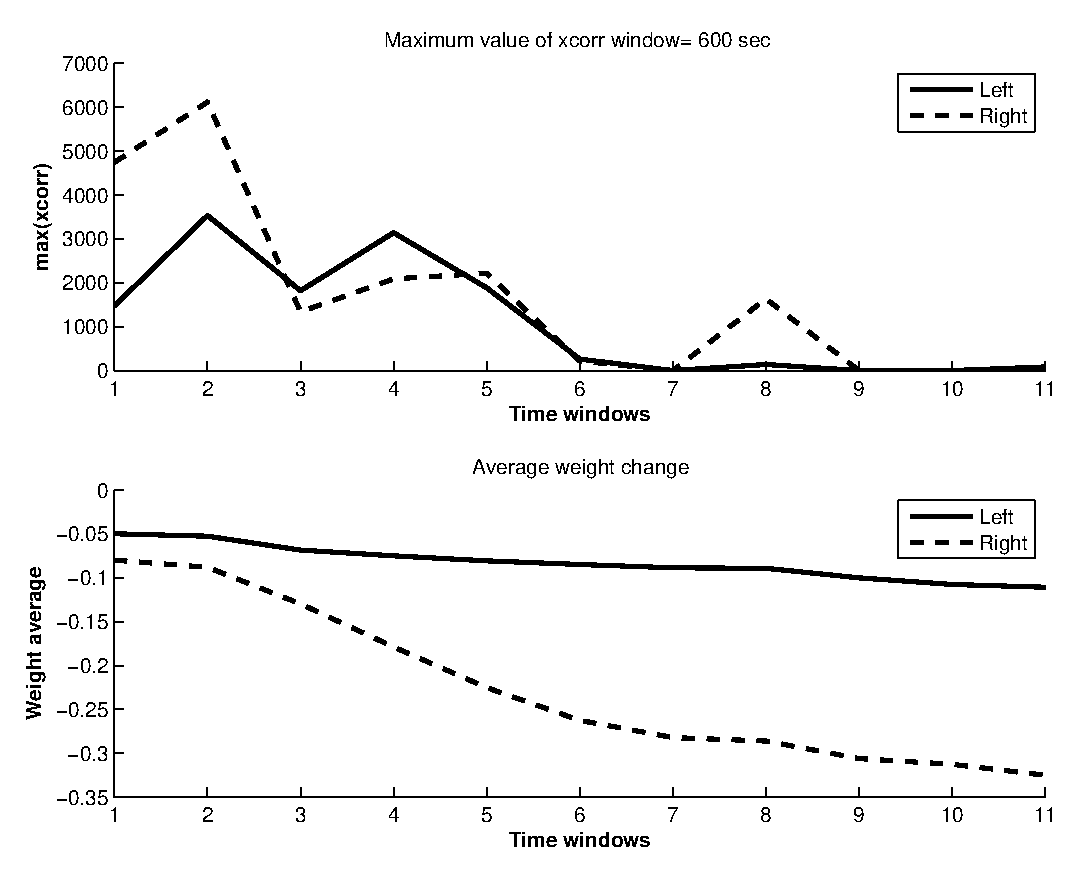
\includegraphics[scale=0.3]{figures/infomeasure/N2/maxcorr_N=0_w=600.eps}}
	\hspace{1pt}
      \subfigure[Energy $E(xcorr_{d}(k))$ for left (straight) and right (dashed) synapses. Measures from agent 0.\label{fig:energy1N2M2}]{
	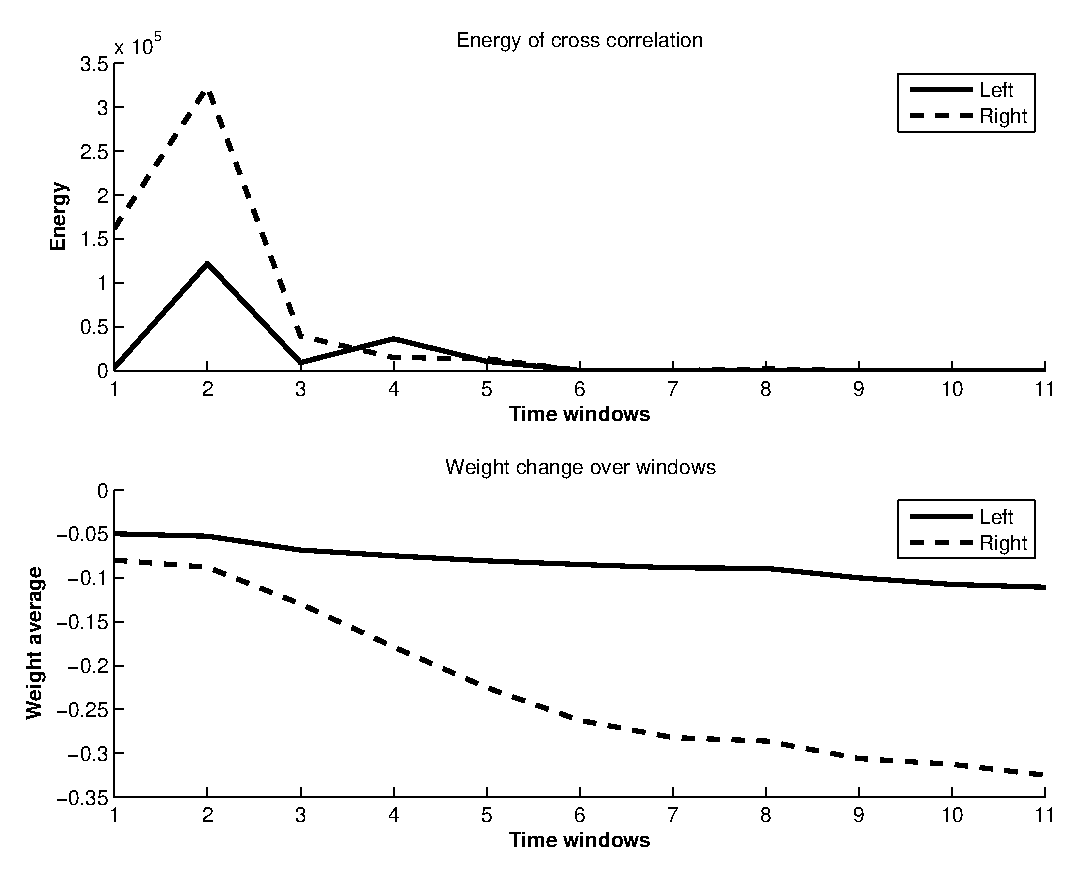
\includegraphics[scale=0.3]{figures/infomeasure/N2/power_xcorr_N=0_w=600.eps}}
      \subfigure[Cross correlation maximum $M(c_{d}(k))$ for left (straight) and right (dashed) synapses. Measures from agent 1.]{
	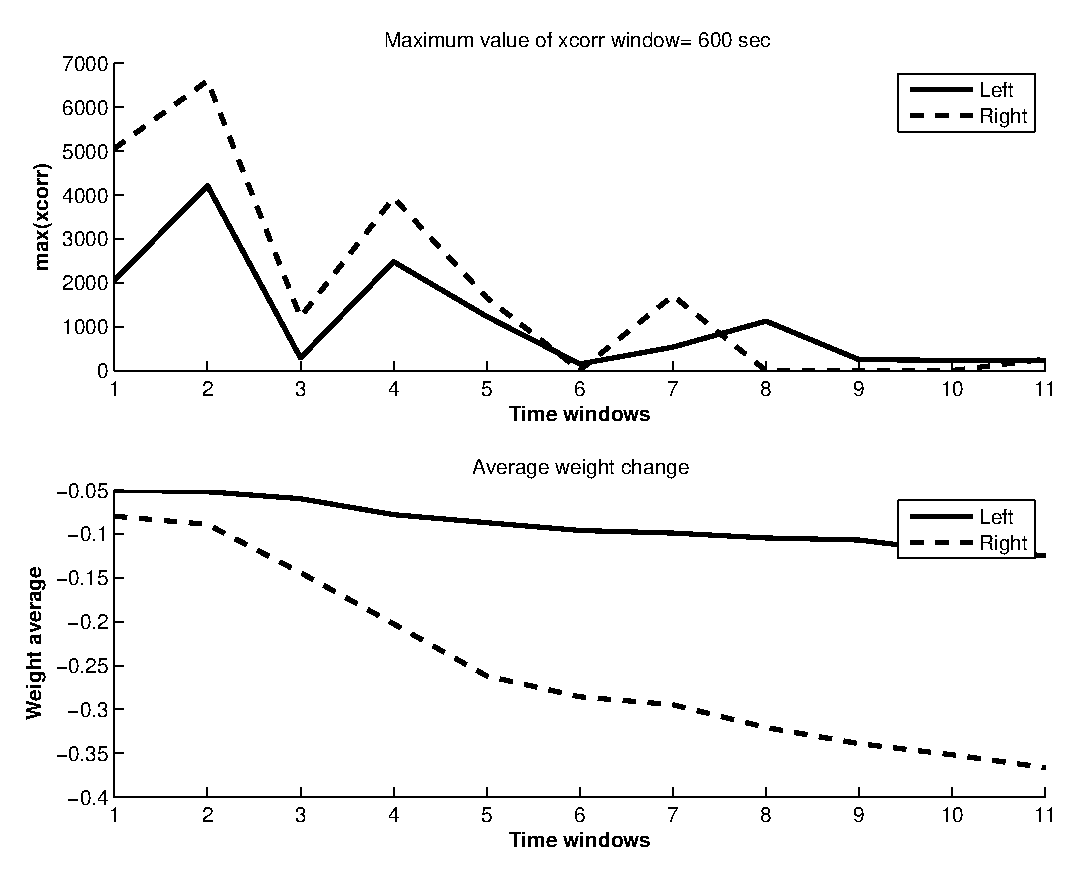
\includegraphics[scale=0.3]{figures/infomeasure/N2/maxcorr_N=1_w=600.eps}}
	\hspace{1pt}
      \subfigure[Energy $E(xcorr_{d}(k))$ for left (straight) and right (dashed) synapses. Measures from the agent 1.\label{fig:energy2N2M2}]{
	\includegraphics[scale=0.3]{figures/infomeasure/N2/power_xcorr_N=1_w=600.eps}}
    \caption[Max correlation for two learning agents]{Information measure analysis for $N=2$ agents
	      and $M=2$ obstacles computed in $k=1,...,11$ time windows.
	      Learning is switched on for all agents when ($k>1$). \label{fig:N2M2}}
  \end{center}
\end{figure}

\paragraph{Experiment with 4 agents and 2 obstacles}
The same considerations apply to the case of 4 agents with 2 obstacles.
Figs.\ref{fig:N4M2a} shows the measures for the first group of 2 agents and Fig.\ref{fig:N4M2b}
shows the measures for the second group of 2 agents.

\begin{figure}[htbp]
  \begin{center}
      \subfigure[Cross correlation maximum $M(c_{d}(k))$ when $N=4$ agents and $M=2$ obstacles for left (straight) and right (dashed) synapses. Measures from agent 0.]{
	\includegraphics[scale=0.3]{figures/infomeasure/N4/maxcorr_N=0_w=600.eps}}
	\hspace{1pt}
      \subfigure[Energy $E(xcorr_{d}(k))$ when $N=4$ agents and $M=2$ obstacles for left (straight) and right (dashed) synapses. Measures from the agent 0.]{
	\includegraphics[scale=0.3]{figures/infomeasure/N4/power_xcorr_N=0_w=600.eps}}
\subfigure[Cross correlation maximum $M(c_{d}(k))$ for left (straight) and right (dashed) synapses. Measures from agent 1.]{
	\includegraphics[scale=0.3]{figures/infomeasure/N4/maxcorr_N=1_w=600.eps}}
	\hspace{1pt}
      \subfigure[Energy $E(xcorr_{d}(k))$ for left (straight) and right (dashed) synapses. Measures from the agent 1. Learning starts after the first window.\label{fig:energylong}]{
	\includegraphics[scale=0.3]{figures/infomeasure/N4/power_xcorr_N=1_w=600.eps}}
    \caption[Max correlation for 4 learning agents A]{
      Information measure analysis for $N=4$ agents and $M=2$ obstacles computed
      in $k=1,...,11$ time windows. Learning is switched on for all agents
      when ($k>1$).\label{fig:N4M2a}}
  \end{center}
\end{figure}


\begin{figure}[htbp]
  \begin{center}
\subfigure[Cross correlation maximum $M(c_{d}(k))$ for left (straight) and right (dashed) synapses. Measures from agent 2.\label{fig:eqlearning}]{
	\includegraphics[scale=0.3]{figures/infomeasure/N4/maxcorr_N=2_w=600.eps}}
	\hspace{1pt}
      \subfigure[Energy $E(xcorr_{d}(k))$ left (straight) and right (dashed) synapses. Measures from the agent 2.\label{fig:energypeak} ]{
	\includegraphics[scale=0.3]{figures/infomeasure/N4/power_xcorr_N=2_w=600.eps}}
\subfigure[Cross correlation maximum $M(c_{d}(k))$ for left (straight) and right (dashed) synapses. Measures from agent 3.]{
	\includegraphics[scale=0.3]{figures/infomeasure/N4/maxcorr_N=3_w=600.eps}}
	\hspace{1pt}
      \subfigure[Energy $E(xcorr_{d}(k))$ for left (straight) and right (dashed) synapses. Measures from the agent 3.\label{fig:energylong2}]{
	\includegraphics[scale=0.3]{figures/infomeasure/N4/power_xcorr_N=3_w=600.eps}}
    \caption[Max correlation for 4 learning agents B]{
	Information measure analysis for $N=4$ agents and $M=2$ obstacles computed
	in $k=1,...,11$ time windows. Learning is switched on for all agents
	when ($k>1$). \label{fig:N4M2b}}
  \end{center}
\end{figure}

As with the previous case the maximum cross correlations of each agent go
to zero when the learning is stable.
For example agent 2 in Fig.\ref{fig:N4M2a}(a,b) stabilises his learning weights
after $k>6$ time windows.
Comparing the maximum of the cross correlation for left and right synapses for all cases,
on average it occurs that $M(xcorr_{left}(k))>M(xcorr_{right}(k))$,$\forall k$:
agents learn more to use the left synapse which therefore is more responsible for the motor
behaviour. As a result the left synapse is more exposed to obstacle signals.
Instead the agent in Fig.\ref{fig:eqlearning} learns equally with both synapses
and in this case $M(xcorr_{left}(k))\cong M(xcorr_{right}(k))$.

An interesting property of the energy $E(xcorr_{d}(k))$ is that in all cases it tends
to zero $E(xcorr_{d}(k)) \cong 0$ when the weight change is stable $Avg(W_{predict,d},k) \cong 0$.
But there are exceptions like cases in Fig.\ref{fig:energylong},\ref{fig:energylong2}
where $E(xcorr_{d}(k)) \cong 0$ for $k>5$ even if the agent is still slowly learning.
This is due to the fine tuning that happens after the initial learning step, essentially
there are still some minor weak collisions which adjust the weights by a small factor.

The energy values can be used to for example agent 2 has a peak in the energy value
as in Fig.\ref{fig:energypeak} because there was an great learning experience at $k=4$,
where the weights' values jumped from $-0.08$ to $-0.18$.
Because the energy value calculates the density of collision events, it can be used
to verify the learning speed of the weight development.

\paragraph{Adding one agent}
When one more agent is added in the simulation at the time window $k=6 s$,
the other agents are ``surprised'' by its behaviour thus they need to adjust their weights.
I am investigating to what extent this behaviour can constitute a sort of primitive social teaching:
if there are some experienced robots the new ones do not have to learn a lot because the others are
compensating for their mistakes.
I can make a hypothesis that there is a critical mass of new agents
when the new ones need to start to learn as well.
The reader must remember that this model is not based on knowledge transfer models of
social colonies: the agents are not learning by imitation.
Learning by imitation requires rather complex functions which are not present in
simple organisms or agents like the one used in this simulation.

% % the energy signal has a peak for every agent: energy is an index of the ``surprise'' or novelty of new signals.
% The new inexperienced agents will be aided by the others to learn: their mates are already good in avoiding so
% for them will it be easier to learn. it is interesting to note that they learn less than others in the same time
% window: this effect is a feature of collaborative colonies where new members are facilitated by the experienced ones.
Fig. \ref{info:agentadd} shows the $M(xcorr_{left}(k)),M(xcorr_{right}(k))$ values
for an experienced agent.
When the new agent is dropped in the arena at time window 6, the agent sees it
by a peak in the cross correlation and thus needs to adjust its weights.  
\begin{figure}[htbp]
  \begin{center}
    \includegraphics[scale=0.65]{figures/infomeasure/agentvariation.eps}
    \caption[Max correlation variation analysis]{A new agent is introduced
	    for t=6, the other agents needs to adjust their weights to the new
	    ``unpredictable'' friend.
\label{info:agentadd}}
  \end{center}
\end{figure}
Unfortunately I did not have any more time to carry extensive analysis, but 
it would have been interesting how the performance of newly introduced agents is affected
by the other experience agents.
Probably the newly introduced agents wouldn't require a lot of learning as the
others are already successfully avoiding.

\subsection{Results: simple case results}
In this simple case there are 2 agents navigating in a rectangular space with
a number of 2 obstacles that are placed randomly in the environment (see Appendix \ref{Appendix:simplesocialsim}). 
Every simulation is run for $T=30$ minutes with a time step of $\varDelta=0.01s$,
the window for the correlation is $W=10$ seconds, therefore $cc(t)$ is computed
for $t=1,2,...,180$.

Anticipatory information is averaged over 100 simulations:
every simulation is randomised in terms of the robots' and obstacles' initial positions.
In the first time window the learning of the agents is switched off and $cc(0)\simeq 0.7071$
because the reflex of the agent is already preventing a full force impact, whereas for
$cc(t>0) \leq 0.7071$ because the impact of the collision can only be equal or decreased.

Fig.\ref{avoidance:resume}(B) shows that AI increases and stabilises to 6 bits when agents
have learned successfully: they are using 6 bits in the predictive loop to reduce the reflex.
Instead non learning agents are not using any bit to reduce the reflex.
The noise visible in Fig.\ref{avoidance:resume} is due to the random repositioning of the
obstacles and random collisions. In a perfect world if agents were able to avoid
perfectly $cc(t)\simeq 0$ and so $AI(t)\rightarrow \infty$.

\begin{figure}[htbp]
\begin{center}
\includegraphics[width=0.6 \textwidth]{infomeasure/simple/infoapplication.eps}
\end{center}
\caption[Max correlation application to a simplified case]{
\textbf{A)} Two agents are learning to avoid obstacles in a closed rectangular world.
At the very left the agent is only reacting to the obstacle thus $AI\simeq0$,
at the very right the agent has learnt successfully how to exploit the predictive
signal $u_1$ to avoid the contact thus $AI > 0$. 
\textbf{B)}  Anticipatory information computed for 2 learning agents.
When learning is stable it reaches a baseline level, $AI(t)\simeq 6$ bits.
If agents are not learning the anticipatory information is low $AI(t)\simeq 0.5$
bits, because $cc(0)\simeq 0.7071$}
\label{avoidance:resume}
\end{figure}

\subsection{Results: simplified social model results}
I apply now the \textbf{AI measure} to a social system such as the one published
in \citet{DiProdiMultiAgent} and described in section \ref{Chapter4:Social adaptation}
where a social system whose task is cooperative food foraging.
As for the avoidance case the agents learn how to use the distal sensors to
approach food (to increase their energy) or other agents (to get their energy).
Agents can forage directly from the food patches (see Fig.\ref{social:learning1}(B))
or reduce the energy of other agents who have previously got food (see Fig.\ref{social:learning1}(D)) .

Thus every agent has two competitive signals:
one from the food patches and one indicating the energy level of the other agents.
Indeed when antennas are in contact with another agent with high energy they produce
impulses on $x_{1,e}$ for far contacts and on $x_{0,e}$ for near contacts,
whereas when they are in contact with a food patch they produce impulses on $x_{1,f}$
for far contacts and on $x_{0,f}$ for near contacts.

Therefore the agent has 2 learning weights $\omega_{1,e}$ for energy and $\omega_{1,f}$
for food that both contribute to the motor output. When the simulation starts,
all agents have $\omega_{1,e}=\omega_{1,f}$ and therefore they approach any object because
according to the situation they will choose the food or the nearby agent.
Nevertheless during the simulation some agents (the seekers) will become more
attracted by the food  $\omega_{1,e}<\omega_{1,f}$, while the others (the parasites)
will become more attracted by the other agents with energy $\omega_{1,e}>\omega_{1,f}$.
An agent changes class or behaviour when the weights are swapped 
i.e. a seeker $\omega_{1,e}<\omega_{1,f}$ becomes a parasite $\omega_{1,e}>\omega_{1,f}$
(or viceversa) thus contributing to the system instability.

The bar diagram of Fig.\ref{social:learning1}(E) shows for every time window how
many times this swap has happened.The system self-stabilises to a number of seekers
and parasites whose number depends on the available resources:
in this case with 4 food resources there are 6 parasites and 4 seekers.
With more resources e.g. 10, there will be 6 seekers and 4 parasites.

Luhmann theorised that sub-systems are formed to reduce the complexity of the perceived environment:
in this case this means that agents are discarding part of the closed loop information.
This process is shown in Fig.\ref{social:learning1} by computing $AI$ for the energy and for the food signal.
The $AI(u_{1,e},u_{0,e})=AI_{energy}$ represents the anticipatory information for the energy attraction and the $AI(u_{1,f},u_{0,f})=AI_{food}$ for the food attraction.
For seekers the $AI_{food}>AI_{energy}$ increases as the system differentiates and conversely for the parasites $AI_{energy}>AI_{food}$.
In term of information it means that seekers are using $AI_{food}-AI_{energy}=2$ bits more to reduce the energy signal, whereas parasites are using $AI_{energy}-AI_{food}=2$ bits more to reduce the food.
\begin{figure}[!htbp]
\begin{center}
\includegraphics[width=0.8 \textwidth]{figures/infomeasure/simple/socialmeasure.eps}
\end{center}
\caption[Max correlation and learning in the simplified case]{B) A parasite is an agent that prefers an energy signal to a food one.  D) A seeker is an agent that prefers a food signal to an energy one produced by another agent. B) For parasites the anticipatory information for food is less than that one of the energy. C) For seekers the anticipatory information for energy is less than that one of
the food. E) There are a total of $N=10$ agents of whom 6 turn into parasites, and 4 turn into seekers after 20 time steps. The system stabilisation is a function of time: at the very
beginning agents are using both signals and their behaviour is unpredictable because they are switching between the 2 competitive behaviours.
After 20 time windows the agents have a more predictable behaviour resulting by the selection of the information. Minor oscillations are again
due to the noise resulting from the interaction between learning agents.}
\label{social:learning1}
\end{figure}


\subsection{Results: differentiation and information measure}
I then computed the information measure $xcorr(k)$ in the same social model \citep{DiProdiMultiAgent}.
The results were compatible again with Luhmann's theory of information reduction
and social differentiation.
The Fig.\ref{info:social} is the outcome of computing the information on a
group of $N=10$ robots and $M=2$ food places.
There are 6 parasites and 4 seekers. In Fig.\ref{info:social} (A) for the 4 seekers
 the information measure of the food's signal is smaller than the average information
 measure of the agent signals. This means that the seekers learn to use only one
signal out of two in order to simplify the closed loop model.
In Fig.\ref{info:social} (B) for the 6 parasites the information measure of the
 agents' signal is smaller than the average information measure of the food's signals.
This means that the parasites learn to use only one signal out of two in order to
 simplify the closed loop model. As I expected when the system is not stable
 Fig.\ref{info:social} (C)  -the agents are switching their class-
the information measure for the food signals and the agent signals are
crossing each other, but when the system becomes stable - switching rate is
approaching 0- I can see that the two information measures start to separate.

\begin{figure}[htbp]
  \begin{center}
    \includegraphics[scale=0.5]{figures/infomeasure/LearningDifferentiation.eps}
    \caption[Max corr computed on the social system]{The information measure computed
      on a group of $N=10$ robots. (A) information measure computed on the 4 seekers
      and compared to the average measure of the 6 parasites. (B) information measure
      computed on the 6 parasites and compared to the average measure of the 4 seekers.
      (C) The switching rate: how many agents changes their class for every time window.
      The system is stable when the switching rate is 0, in this case after 7 windows.
      \label{info:social}}
  \end{center}
\end{figure}

Luhmann theorised that in society, specialised groups emerge when they reduce
the uncertainty of the environment-system boundary in a recursive process.
The model's results validate his theory because agents are selecting to use one
information rather than the other one to simplify the model of the environment's loop.

\subsection{Discussion}
Devising a measure of information for learning agents in a closed loop is a challenging task.
Previous approaches in the literature are all based on the concept of Shannon's
entropy applied to adaptive controllers.
There are 3 main problems in using Shannon's entropy:
\begin{itemize}
 \item it ignores semantics when dealing with transmitted data: when a sequence of
symbol is transmitted, every symbol carries the same importance, only their probability
 of occurrence plays a role in Shannon's model.
\item is not suitable for closed loop: joint and disjoint probabilities change continuously
 in the closed loop and therefore they must be estimated continuously.
\item probability encoding discards temporal information: positive and negative phase
 delay induces the same variation in the mutual information measure (see Appendix A).
\end{itemize}
\citet{PhysRevLett.84.1156} consider the perception action-loop
 in terms of a communication channel-like model.
Also \citet{organizationInfo} recently has been using the
same approach: the perception-action loop enables an agent to use its actuators
as a channel to transmit information into the environment.
The information can later be acquired from the environment by the same agent or other agents.
 In our measure there is no such transfer channel: temporal information
relevant to the agent is computed only at the inputs which contains the feedback
 of the outputs. It is simple and easy to compute and it does not require the modelling of the agent's
 controller as an information channel.
Recently, \citet{shannonSemantic} has been working on evolving sensors and has
 introduced an operational notion of Shannon-type quantification of relevant information:
\begin{itemize}
 \item it quantifies relevance with respect to a given agent or decision system.
 \item it yields a measure for the usefulness of sensors or about an agent's state
of knowledge with respect to a POMDP (partial observable markov decision process)
\end{itemize}
The problem of this approach is that it requires a discrete formulation of
an agent, and its application to a general controller is not possible.
The limit of the \textbf{maxcorr} measure is that it is dependent on the particular implementation
of our controller and cannot be applied to other adaptive algorithms unless
they are based on a similar temporal input structure.
The limit of the \textbf{AI measure} is that although it quantifies the learning
behaviour in terms of bits, it does not provide an axiomatic framework and
thus can be mathematically weak.
Therefore in Section \ref{Chapter6:Information Flow}, the author developed a more
advanced measure based on the concept of information flow which is inspired by the
work of \citet{LungarellaInformation}.




\section{Information flow for adaptive controllers \label{Chapter6:Information Flow}}

This Section describes an improvement of the previous information measure described
in Section \ref{Chapter5:Max Corr Input}.
The new theoretical framework, based on Shannon's communication theory
 and on Ashby's law of requisite variety, is suitable for artificial agents
using predictive learning.
The framework quantifies the performance constraints of a predictive adaptive
controller as a function of its learning stage.
In addition, I formulate a practical measure, based on information flow,
that can be applied to adaptive controllers which use Hebbian learning,
input correlation learning (ICO/ISO) and temporal difference learning.
The framework is also useful in quantifying the social division of tasks in a
social group of honest, cooperative food foraging, communicating agents.
Simulations are in accordance with Luhmann, who
suggested that adaptive agents self-organise by reducing the amount of sensory
information or, equivalently, reducing the complexity of the
perceived environment from the agent’s perspective.

\subsection{Introduction: Ashby's theory}

Information measures are usually defined for input/output systems where
they determine the quality of the transmission. Behaving agents,
however, act as closed loop systems in which there is no clearly defined
difference between input and output.
What matters most for the organism is to compensate for disturbances introduced by
 the environment in the perception action loop. If there is no disturbance,
the organisms cannot differentiate between themselves and the environment.
Consequently, the concept of information in these
systems needs to be revised \citep{RadicalConstruct}.

A method for defining closed loop information has been proposed by \citet{Ashby1956:IntroCybernetics}
the so called \textit{requisite variety} .
The measure is based on the premise that closed loop systems aim to maintain
a desired state.
The goal of a feedback loop is then to minimise the deviation from the desired
state i.e. the number of bits required to successfully
compensate a disturbance acting on the forward loop. In this
way, the method quantifies the variety, or bits, originating from the
disturbance. For example, if the disturbance has a variety of 10 bits and
survival requires a desired state of 2 bits, then the reaction to that disturbance
must provide a variety of 8 bits.
Ashby then proved that error controlled closed loop systems (like PID controllers 
discovered by \citet{PID}) cannot achieve perfect regulation.
More recently, \citet{PhysRevLett.84.1156} in Theorem 10 proved
that the entropy reduction achieved by a closed loop system
is bounded by the entropy reduction achieved by the open loop control plus
the mutual information gathered by the estimation of the state.
However the advent of predictive controllers, such as Q-learning \citep{TD},
that predict future states, requires an extension of the information theory for
predictive learning.

In this section, I present an extension to
the law of requisite variety, called \textit{the predictive requisite variety},
that quantifies the theoretical limits of control (as well as providing a performance index)
for predictive adaptive controllers.
I argue that a predictive adaptive controller acts as a reactive system before learning
and as an open feed-forward system after learning.
A reactive system comprises an error controlled closed
loop and is non optimal because it only reacts after a
deviation from its desired state has happened.
The environment usually contains predictive signals which can help the agent to
react before the error is presented \citep{Verschure2003}. Thus, bio inspired controllers
can be provided with a predictive signal (like vision) and a reflexive signal (like touch).
Learning then has the task of avoiding the trigger of the reflexive reaction -
thus creating an open loop forward controller which discards
the information of the reflexive signal.

Learning is then quantified by the increase in the information flow of the predictive
loop and by a corresponding decrease in the information flow of the closed loop.
Information flow, or transfer entropy, is not a new idea (see for
example \citep{infoFlow,transferEntropy}) but it has never been applied to
predictive agents in order to assess their learning performance.
The analysis of a predictive agent with a single behaviour, say for
example obstacle avoidance, can be done by calculating the information flow of the
sensory-motor loop.

Analysis becomes more complicated when an agent is provided with a set of
competitive behaviours in a social scenario where agents use predictive
learning- see, for example, ISO \citep{Porr2003rsoc} or ICO \citep{Porr2006ICO}
- and are therefore learning from each other.
The task of the social system in this analysis is cooperative food foraging
in which every agent has 3 adaptive behaviours which are:
avoidance for obstacles, attraction to food disks and attraction to others with food.
Agents communicate honestly, always signalling to others when they find food.
When the social system is adapting, it self-organises into 2 sub-systems each
described by a dominant behaviour: seekers have a dominant attraction for food
disks, parasites have a dominant attraction to others with food.
The information flow explains how the social system divides itself
into sub-systems by looking at the information processing of every agent.
\citet{Luhmann95} proposed that differentiation of social systems is
caused by a decrease in information processing of each subsystem and this
is consistent with my information flow measurements.

The following sections covers the topics: regulation and
entropy (as defined originally by Ashby), a new information measure for predictive
learning, a simulation model with social adaptive agents, results and a discussion.


\subsection{Methods: Ashby's law of requisite variety}
First, it is necessary to review Ashby's Law of Requisite Variety for the forward
(see Fig.\ref{fig:ashby1}(B)) and closed loop controller (see Fig.\ref{fig:ashby1}(A)).
Fig.\ref{fig:ashby1} uses the same notation introduced by Ashby:
\begin{itemize}
 \item \textbf{D} is the finite state machine whose states are the disturbances from the environment
 \item \textbf{E} is the finite state machine whose states are the essential variables partitioned
in $E= \eta \cup \overline{\eta}$, where $\eta$ is a partition of desired states or
 goals of the organism and its complementary partition $\overline{\eta}$ represents
 the non-desired states.
 \item \textbf{R} is the finite state machine whose states are the available regulations/actions that the organism can perform
 \item \textbf{T} is the finite state machine whose states are the set of possible states of the environment
\end{itemize}
In this work I consider deterministic finite state machines but the analysis
can also be extended to Markov processes as in \citet{FSMbook}. It is very important
for my analysis to understand that only the forward controller can achieve
perfect regulation whereas the closed loop controller cannot because the reflex
always comes too late.
\citet{Ashby1956:IntroCybernetics} stated that a good controller $R$ blocks
 the flow of variety\footnote{Ashby defines variety precisely as the number
of different states a variable can take and is equivalent to Shannon's
entropy $H$ measured in bits.} from disturbances $D$ to essential variables
 $E$: if R is a regulator, the insertion of R between D and E decreases the
 variety that is transmitted from D to E.
An organism can be described by a body $R$ with goals to be achieved $\eta$
 and an environment $T$ which forms a closed loop between actions and sensors.
As an analogy, the organism is a perfect regulator if is able to keep
 the essential variables E within a desired sub-set $\eta$ in spite of the
disturbances D -thus having a null entropy for E, $H(E)=0$.

\paragraph{Definition and properties}
If no regulator $R$ is provided (see Fig.\ref{fig:ashby1}(C)), the disturbance D
tends to drive $E_0$ outside a set of desired states $\eta$ by means of the
environment $T$.
Thus, in the worse case, the disturbance completely controls the status of the organism:
\begin{equation}
H(D)=H(E_0)\label{eq:initial}
\end{equation}
which means all the disturbances is transferred intact to the organism.
\begin{figure}
\begin{center}
\includegraphics[scale=0.3]{lawvariety/lawvariety1_fonts}
\caption[Law of requisite variety for learning and non learning agents]{(A)
The organism with a closed loop controller. (B) The same organism with an forward
controller. (C) The organism before regulation. (D) An adaptive controller is a
 mix of forward and closed loop control. Every block is a finite state machine
whose inputs are indicated by incoming arrows and outputs are indicated by
outgoing arrows. \label{fig:ashby1}}
\end{center}
\end{figure}
The regulator $R$ can be connected in a feed-forward configuration as in
Fig.\ref{fig:ashby1}(B) or in a closed loop configuration as in Fig.\ref{fig:ashby1}(A).
The performance of the forward regulator is measured by the maximum entropy
reduction $\Delta H^{max}_{forward}$ which is the difference between the entropy
of the essential variable $H(E_0)$ before regulation and after regulation $H(E)$.
\begin{equation}
\Delta H^{max}_{forward}=H(E_0)-min H(E)\label{eq:Hreduction}
\end{equation}
The maximum entropy reduction in the forward condition $\Delta H^{max}_{forward}$
 can be calculated by using the Law of Requisite Variety:
\begin{equation}
H(E)\geq H(D)+H(R|D)-H(R)\label{eq:lawvariety1}
\end{equation}
where $H(R|D)$ is the regulator noise\footnote{If the controller is not noisy $H(R|D)=0$}.
Thus:
\begin{equation}
\Delta H^{max}_{forward}=H(R)-H(R|D)\label{eq.deltaforward}
\end{equation}
because combining Eq.\ref{eq:Hreduction} and Eq.\ref{eq:lawvariety1} gives:
\begin{equation}
\Delta H^{max}_{forward}=H(E_0)-H(D)-H(R|D)+H(R)
\end{equation}
Considering the initial condition in Eq.\ref{eq:initial} I obtain Eq.\ref{eq.deltaforward}:
\begin{equation}
\Delta H^{max}_{forward}=H(D)-H(D)-H(R|D)+H(R)=H(R)-H(R|D)
\end{equation}
The quantity $\Delta H^{max}_{forward}$ in Eq.\ref{eq.deltaforward} tells us that
better performance can be achieved by either increasing the regulation entropy
$H(R)$ or by decreasing the controller noise $H(R|D)$.
A closed loop controller cannot achieve perfect regulation ($H(E)=0$) as it requires
a deviation from the desired state $\eta$ to work $H(E)>0$.
Thus, the disturbance transmits all its entropy to the essential variable $H(D)=H(E)$
and no entropy reduction can be achieved:
\begin{equation}
\Delta H^{max}_{close}=0\label{eq.deltaclosed}
\end{equation}
When $H(E)=0$, $R$ blocks the information flow in the channel $D\rightarrow E$
and thus no information is transmitted to $R$ for the regulation task: the regulator $R$
is asserting a perfect control on $E$ without knowing the status.
This property was proved by absurd in \citet{Ashby1956:IntroCybernetics}.
In the next section I extend the law of requisite variety for adaptive controllers.

\subsection{Methods: the law of adaptive requisite variety}
An adaptive controller (see Fig.\ref{fig:ashby1}(D)) is a mix of a forward
\citep{feed-forward} and closed loop controllers \citep{PID} because $R$ now has
2 inputs: $D$ and $E$. I can think of $D$ as a predictor of the deviation
of $E$, because $D$ transfers its entropy to $E$ by means of the environment $T$.

In order to explain the new law, I introduce the mutual information $I(E,R)$
for the closed loop channel $E\rightarrow R$ with the corresponding channel
capacity $C_{E,R}$:
\begin{eqnarray}
I(E,R)=H(E)+H(R)-H(E,R)\\
C_{E,R}=\max_{p(E)} I(E,R)
\end{eqnarray}
the mutual information $I(D,R)$ for the forward channel $D\rightarrow R$ with the
corresponding channel capacity $C_{D,R}$:
\begin{eqnarray}
I(D,R)=H(D)+H(R)-H(D,R)\\
C_{D,R}=\max_{p(D)} I(D,R)
\end{eqnarray}
The channel capacity of the regulator channel $D \rightarrow T$ is then $C_{R,T}$.

The adaptive controller (denoted ada) begins as a closed loop controller with
$\Delta H^{max}_{ada}(before)=H^{max}_{close}$ (see Eq.\ref{eq.deltaclosed}) as
 it mainly uses the $E\rightarrow R$ reflex channel and blocks the $D \rightarrow R$
predictor channel whose mutual information is very low. In summary:
\begin{eqnarray}
0<I(E,R)\leq C_{E,R}\\
I(D,R)\simeq 0\\
\Delta H^{max}_{ada}(before)=0
\end{eqnarray}
The adaptive controller achieves perfect regulation (see Eq.\ref{eq.deltaforward}) when
\begin{equation}
\Delta H^{max}_{ada}(after)=H^{max}_{forward}
\end{equation}
because it blocks the $E\rightarrow R$ reflex channel and opens the $D\rightarrow R$
 predictor channel. To summarise:
\begin{eqnarray}
0<I(D,R)\leq C_{D,R}\\
I(E,R)\simeq 0\\
\Delta H^{max}_{ada}(after)=H(R)-H(R|D)
\end{eqnarray}
If I assume realistically that the regulator has a common channel capacity
$C_{E,R}=C_{D,R}=C_{R,T}$, the constraint for learning becomes:
\begin{equation}
I(E,R)+I(D,R) \leq C_{R,T}\label{eq.constraint}
\end{equation}
thus an adaptive controller can achieve optimal regulation $\Delta H^{max}_{ada}(after)$
when it is able to compensate the mutual information of the closed loop $I(E,R)$
with the mutual information of the forward controller $I(D,R)$.
An imperfect regulator will likely work in the sub-optimal regime $I(D,R)<I(E,R)$.
So to quantify the performance of an adaptive predictive controller I have to
compute the mutual information $I(D,R)$ and $I(E,R)$.
This is however not always possible because it is hard to identify the reflex
 channel and the predictor channel.
Therefore in the next section I use an approximation of these 2 quantities
using the concept of information flow.

\subsection{Methods: information flow for adaptive predictive controllers}
Looking at Fig.\ref{fig:ashby1}(D), I can estimate $I(E,R)$ by computing the
information flow of the reflex-output channel $Z^n \rightarrow  U_0$ and $I(D,R)$
by computing the information flow of the predictive-output channel $Z^n \rightarrow  U_1$.
I denoted them as:
\begin{eqnarray}
MI^n_{U0}=I(Z^n,U_0) \leftrightarrow I(E,R)\label{eq.mi0}\\
MI^n_{U1}=I(Z^n,U_1) \leftrightarrow I(D,R)\label{eq.mi1}
\end{eqnarray}
where $U0$ is the reflex input, $U1$ is the predictor input and
$Z^{n}$ the extended output:
\begin{equation}
Z^n=[z(k) z(k+1)\dots z(k+n-1)]
\end{equation}
which contains $n$ outputs of the agent and $U$ the random variable describing the
temporal signal $u(k+n)$ which is the input of the agent resulting from
previous actions as described in \citet{organizationInfo,quantifyInfo}.
Fig.\ref{methods:ico1}(A) shows an organism composed of 3 ICO \citep{Porr2006ICO}
controllers and the corresponding information flow measures for every controller.
Each ICO controller takes 2 continuous inputs $U0,U1$ and one continuous output $Z_{n}$.

ICO correlates the predictive signal $u_{1}$\footnote{$u_{1}$ and $u_{0}$ indicates
temporal signals $u_{1}(t)$ and $u_{0}(t)$} with the derivative of
the reflexive signal $u_{0}$ according to the formula:
\begin{equation}
 \frac{d\omega_1}{dt}=\mu \cdot u_1 \cdot \frac{du_0}{dt}
\end{equation}
where $\omega_1$ is the gain of the predictive signal $u_{1}$ and $\mu$ is the
learning speed (see Fig.\ref{methods:ico1}(C)).

Since the ICO controller works in continuous mode, the input and output signals
must be discretised in order to compute the information flow and channel capacity (see Simulation Details).
The two measures $MI^n_{U0},MI^n_{U1}$ are used to compute the channel capacities $C_{E,R}$ and $C_{D,R}$:
\begin{eqnarray}
\zeta^n(Z^n \rightarrow U0)=\max_{p(Z^n) } MI^n_{U0}  \leftrightarrow C_{E,R} \label{eq:c0}\\
\zeta^n(Z^n \rightarrow U1)=\max_{p(Z^n) } MI^n_{U1}   \leftrightarrow C_{D,R} \label{eq.c1}
\end{eqnarray}
In the simulations in the next section, I will estimate the mentioned quantities
for individual agents of a social group.

\subsection{Methods: information flow applied to MISO controller}
The previous measures are applied to a social system where all agents learn continuously
from each other and from the environment. This scenario is very interesting because
the social system is able to self-organise by forming 2 sub-systems with task division.
The social system described in \citet{DiProdiMultiAgent} is composed of $N$
identical agents and $M$ food disks randomly placed in a square world for
every simulation (for more details see Appendix \ref{Appendix:InfoFlowSimDetails}).
Food disks contain a certain amount of food that is depleted
when an agent finds it. The task is cooperative food foraging.
The simulated agent is shown in Fig.\ref{methods:ico1}(B) and has also been used
by \citet{Kulvicius2009:analysisdifferential}:
it is a Braitenberg \citep{Braitenberg} vehicle with 2
lateral wheels and 2 antennas. By default the agent drives straight forward,
with speed $v=1$ units per time step. It has 2 sensor-pairs, near contact
antennas and far contact antennas.

Every agent has a MISO (multiple inputs single output) controller and a variable
of 1 bit for the food status. The agent has 3 competitive tasks: avoid obstacles
(empty food disks and other agents without food), find food from the disks,
find foods from other agents with food.
The MISO is composed of 3 parallel ICO controllers (see Fig.\ref{methods:ico1}(A))
which are provided with a reflex input error $u_0$, a predictive signal error $u_1$,
a learnt weight $\omega_1$ and an output $z$.
The outputs of the 3 ICO controllers are summed to $z=z_{Av}+z_{Fo}+z_{Af}$
\footnote{Av stands for obstacle avoidance, Fo for food attraction and Af for attraction to others with food}
which gives the steering angle: $z=0$ the robot goes straight forward at speed $v$,
 $z>0$ the robot rotates clockwise, $z<0$ the robot rotates anti-clockwise.
\begin{figure}
\begin{center}
\includegraphics[width=1.0\textwidth]{lawvariety/controller_fonts}
\end{center}
\caption[MISO controller with triple behaviour]{(A)
MISO controller composed of 3 stacked ICO controllers for avoidance, food attraction
 and attraction to others.
The output of every controller is summed to $z$. For every controller/behaviour the
 pair of mutual information is computed
between the output and the input $MI^n_{U0},MI^n_{U1}$. (B) Agent with short antennas
 (reflexive inputs, $x_0$) and
long antennas (predictive inputs, $x_1$). The agent is learning to avoid obstacles.
The motor reaction will reduce the
intensity of the painful reflex $x_0$ as well as delay its occurrence.
(C) Schematic diagram of the input correlation learning
rule and the signal structure \citep{Porr2006ICO}. The $u_0$ and $u_1$ are,
 respectively, the difference between the filtered
 values of the left and right antennas of the agent. During learning the $u_0$
peak will be shifted in time and reduced in
amplitude as the agent learns successfully by increasing the predictor
gain $\omega_1$. \label{methods:ico1}}
\end{figure}
Every simulation is run for $0\leq k \leq 6 \cdot 10^5$ time steps and is divided in 3 stages.
At every stage, each agent produces 6 input time series and 1 output
 time series $z(k)$ which means that I can calculate the information flow for every pair of
reflex-output and predictor-output: $MI^n_{U0},MI^n_{U1}$.
For a single simulation:
\begin{enumerate}
 \item for $0\leq k_1\leq 2 \cdot 10^5$ all agents are reactive ($\mu=0$).
	For each agent $i={1,...,N}$ I have 3 pairs of information flow:
	\begin{enumerate}
	\item avoidance: $MI^n_{Av,U1},MI^n_{Av,U0}$
	\item food attraction: $MI^n_{Fo,U1},MI^n_{Fo,U0}$
	\item others attraction: $MI^n_{Af,U1},MI^n_{Af,U0}$
	\end{enumerate}
 \item for $2 \cdot 10^5<k\leq 4 \cdot 10^5$: every agent is learning $\mu=1.0$
and the weight for every ICO controller $\omega_{1,Av}$,$\omega_{1,Fo},\omega_{1,Af}$ is increasing.
 \item for $4\cdot 10^5< k_3\leq 6 \cdot 10^5$: every agent stops learning $\mu=0.0$
and is using the last weight set at $k=4\cdot 10^5$. For each agent I compute again
the 3 pairs of the $MI^n$.
\end{enumerate}

The channel capacities for every agent are computed by providing each isolated output
$z=z_{Av}$,$z=z_{Fo}$,$z=z_{Af}$ with a source of independent randomness during a simulation
of $2\cdot 10^5$ time steps for every case.
Then I apply the Blahut-Arimoto algorithm \citep{Blahut1,Blahut2} with a bound
 error of $\varepsilon =10^{-11}$ and 5000 maximum iterations to estimate the channel
 capacity for every agent in the reflex-output loop
$\zeta^n(Z^n_k \rightarrow U0)$. There is no difference between $\zeta^n(Z^n_k \rightarrow U0)$
of every agent so I define $\zeta^n_{all}$. To compute the capacity for the predictor-output loop
$\zeta^n(Z^n_k \rightarrow U1)$ I use the same approach but preset the weights of every agent
to an arbitrary high value to simulate perfect learning:
\begin{equation}
\omega_{1,Av}=10.0,\omega_{1,Fo}=10.0,\omega_{1,Af}=10.0
\end{equation}
and I obtain the same results
\begin{equation}
\zeta^n(Z^n_k \rightarrow U1)=\zeta^n(Z^n_k \rightarrow U0)=2.0
\end{equation} for $n \geq 2$ as anticipated in Eq.\ref{eq:c0},\ref{eq.c1}.

\subsection{Results}
The results of this sections are based on a set of 100 simulations with 
$N=10$ agents and $M=5$ food disks.
All agents start with the same weights for every ICO controller $\omega_{1,Av}=0.1$,
$\omega_{1,Fo}=0.1,\omega_{1,Af}=0.1$.
In stage 3 there are 5 agents with $\omega_{1,Af}<\omega_{1,Fo}$ and 5 agents with
$\omega_{1,Af}>\omega_{1,Fo}$. 
The first group of agents - identified by the indexes 1,7,3,9,2 -
is characterized by a strong attractive 
behaviour for the food disks (see Fig.\ref{fig:summary} (B)), whereas the second group 
- identified by the indexes 5,8,4,10,6 - is characterized
by a strong attractive behaviour for others agent with food (see Fig.\ref{fig:summary} (E)). 

I estimate the $MI^4$ in stage 1 and stage 3 for every agent by using the corrected
 standard deviation formula \citep{Rouslton}. Before learning (Fig.\ref{fig:summary} (A),(D))
the reflex-output loop predominates over the predictor-output loop for both the
food attraction behaviour and the others attraction behaviour:
\begin{eqnarray}
MI^4_{Af,U1}<MI^4_{Af,U0} \simeq 0.0025\\
MI^4_{Fo,U1}<MI^4_{Fo,U0}\simeq 0.001.
\end{eqnarray}

After learning (stage 3). the configuration is reverted and the predictor-output
loop dominates the reflex-output loop for both behaviours as in
Fig.\ref{fig:summary}(B), (E):
\begin{eqnarray}
MI^4_{Af,U0}\ll MI^4_{Af,U1}\\
MI^4_{Fo,U0} \ll MI^4_{Fo,U1}
\end{eqnarray}

This result matches my expectations in terms of the increase of $I(D,R)$ and
decrease of $I(E,R)$.
If I compare the $MI^4_{Af,U1}$ in Fig.\ref{fig:summary}(B) to $MI^4_{Fo,U1}$
in Fig.\ref{fig:summary}(E) I can see that the agents with indices 1,2,3,4,5
(parasites) have a larger weight $\Delta W_{Af}\simeq 2.0$ (see Fig.\ref{fig:summary}(C))
for the attraction to others and, therefore, a larger information flow
$MI^4_{Af,U1}>MI^4_{Fo,U1}$, whereas agents with indices 6,7,8,9,10 (seekers)
 have a larger weight change $\Delta W_{Fo}\simeq 2.0$ for the food attraction
and so a bigger $MI^4_{Fo,U1}>MI^4_{Af,U1}$.

Thus, the information measure is directly correlated with the weight change and
can be used to quantify the learning performance of a single agent before and
after learning. However, it can also be used to quantify the dominant behaviour
and, consequently, the self-organising properties of social systems.


\begin{figure}
\begin{center}
\includegraphics[width=1.0\textwidth]{lawvariety/allpanel}
\begin{small}
\caption[Information flow before and after learning]{
\textbf{(A)} Information flow before learning for attraction to others $MI^4_{Af,U1}$ (grey bars)$,MI^4_{Af,U0}$ (black bars)
expressed in bits.
\textbf{(B)} Information flow after learning for attraction to others in bits.
\textbf{(C)} Weight difference for every agent: $\Delta W_{Af}=\omega_{1,Af}-0.1$, $\Delta W_{Fo}=\omega_{1,Fo}-0.1$
\textbf{(D)} Information flow before learning for attraction for food $MI^4_{Fo,U1}$ (grey bars), $MI^4_{Fo,U0}$ (black bars) in bits.
\textbf{(E)} Information flow after learning for attraction for food in bits. Error bars are centred on the average for 100 simulations.
The error width is equal to the maximum-minimum interval of the computed measures over 100 simulations.
The agent's indexes are only reported for 1 simulation, because for the rest of the simulations the order outcome
was shuffled. In this set of simulations there were $N=10$ agents with $M=5$ food resources.
\label{fig:summary}}
\end{small}
\end{center}
\end{figure}

In Fig.\ref{fig:Cmax} I measure the efficiency of the reflex-output and predictive-output 
loop $MI^4_{Av,U1},MI^4_{Av,U0}$ for the avoidance behaviour in relation to the capacity 
for the agents $\zeta^4_{all}=2.0$. Fig.\ref{fig:Cmax}(A) shows
that before learning $MI^4_{Av,U0}$ is using 0.25\% of the full channel capacity and 
Fig.\ref{fig:Cmax}(B) shows that after learning $MI^4_{Av,U1}$ is using about 0.45\% of the channel capacity.
\begin{figure}
\begin{center}
\includegraphics[width=0.8\textwidth]{lawvariety/percentage}
\caption[Information flow and capacity]{
(A) Efficiency for every agent of the reflex-output and predictive-output loop
 in terms of capacity before learning (stage 1):
$MI^4_{Av,U0}/\zeta^4_{all} \%$ (dark bars),
$MI^4_{Av,U1}/\zeta^4_{all}\%$ (grey bars).
(B) Efficiency after learning (stage 3).  \label{fig:Cmax}}
\end{center}
\end{figure}
The $MI$ of order $n=1,2,3$ does not provide enough discrimination for the previous
analysis because the output history of the agent is too short to be correlated with the inputs.
The capacity $\zeta^n_{all}$ takes its maximum of 2 bits when $n \geq 2$.
\subsection{Discussion}
In summary, I have introduced an extension to Ashby's
requisite variety theory called the law of adaptive requisite variety,
computed the information flow to measure the learning performance for agents with
competitive behaviours and found the relation between the efficiency of the information flow $MI$ and the weight change
of the adaptive controller $\Delta \omega_1$.

I also linked the information approach to the Luhmann theory that sub-systems are formed
to reduce the perceived complexity of the environment.
In my simulations, after the learning experience 5 agents have a dominant
attraction behaviour for food disks (seekers) and 5 have a dominant attraction
behaviour for others (parasites).
The seekers mainly use the predictive information of the food disks while the
parasites mainly use the predictive information of the others who posses food.
Thus, the conclusion is that predictive learning in a social context
leads to the formation of subsystems. This can be demonstrated with the help of my approach.

While \citet{organizationInfo,polaniEmpowerment} and \citet{LungarellaInformation,optionsOpen}
used the empowerment measure as a general cost function to optimise the agent's
behaviour or evolution, I use it as the upper bound of the MI to measure the efficiency of the sensory-motor loop use.
\citet{AyClosedLoop} uses an adaptive controller which maximises
the excess entropy (the mutual information
between past and present) at the input side to achieve a working regime exploratory
and sensitive to the environment.
I can calculate the MI for this case by considering the reflex as the present input
and the predictor as the past history.
My approach is not restricted to MISO controllers.
\citet{Kulvicius2009:analysisdifferential} measures the temporal input development, the
output and path entropy of the adaptive agents to study the optimality of the antenna ratio for an avoidance task,
thus completing the tools required to evaluate a single task controller.

The following section \ref{Chapter7:Q learning application} contains some experiment
regarding the application of the mutual information to a Q-learning agent to
verify that this approach is feasible also with reward based learning.
After that, the section \ref{Chapter8:Predictive Performance} introduces a mono-dimensional
measure called Predictive Performance which summarises the learning performance
with a singular scalar measure.
This is necessary to avoid the multi dimensional analysis based on the mutual information
of the predictor and reflex pathway: for every behaviour, like the food attraction,
I have to look at both the values $MI^4_{Fo,U0},MI^4_{Fo,U0}$.
Things get more complicate when it is necessary to compare the performance of 
different agents, because then there is no normalisation basis for doing so.
Another issue is the absolute performance in terms of regulation: how can I identify
if one agent despite its efforts was able to keep its desired state.
These questions will be answered in the section \ref{Chapter8:Predictive Performance}. 





\section{Introduction: information flow in Q-learning \label{Chapter7:Q learning application}}

This Section applies the information flow to an artificial agent
which uses reinforcement learning for an an obstacle avoidance task.
The purpose of the experiment is to prove that the same principles introduced
in the previous chapters apply to such a different on-line learning principle.
I will introduce first reinforcement learning, then describe the
robot-environment task with the learning controller and finally shows the
result of the application of the information flow.

\subsection{Methods: reinforcement learning }

Reinforcement learning \citep{TD} is characterised by a learning problem: an agent
learns from its interactions with the environment to achieve a goal.
Any method that is suited to solve this problem, is considered to be
a reinforcement learning method.
A reinforcement learning system is composed by:
\begin{itemize}
 \item the agent: the learner and decision maker decides to make an action $a_t$
 \item the environment: what interacts with the agent. It is described by a
state $s_t$ and gives a reward $r_{t+1}$ for each action.
 \item a policy $\pi_t$: a mapping from perceived states of the environment to
actions to be taken when in those states
 \item a reward function: a mapping from perceived states (or state-action pairs)
of the environment to a reward (a number).
The reward defines what are the good and bad events for the agent.
 \item a value function $V^{\pi}$: a mapping from perceived states to a value
which represents the expected total amount of reward that can be accumulated
over the future.
 \item optionally a model of the environment
\end{itemize}

The agent and the environment interact in time steps $t=0,1,2,3,4$
\footnote{for simplicity we assume a digital simulation but it can be extended
to the continuous case see \citep{TDrealtime}}.
At each time step t, the agent produces a representation of the environment's state,
$s_t \in S$, where  $S$
is the set of possible states and on that basis it takes an action $a_t \in A(s_t)$,
where $A(s_t)$ is the set of available actions in the state $s_t$.
One step later, the agent receives a numerical reward $r_{t+1}\in R$ and
find itself in a new state $s_{t+1}$.
At each time step the agent implements a mapping from states to probabilities
of selecting each possible action. The probabilities are
computed thanks to the agent's policy, where $\pi_t(s,a)$ is a mapping from
each state $s$ and action $a$ to the probability
of taking action  $a_t=a$ when in state $s_t=s$.
The vast majorities of reinforcement learning algorithms are based on estimating
the value function that estimates
how good it is for the agent to be in a given state. The positivity is defined in
terms of future rewards.
Thus, the value function $V^{\pi}(s)$, is the expected return when starting in
$s$ and following $\pi$ thereafter:
\begin{equation}
 V^\pi(s)=E{R_t|s_t=s}
\end{equation}
$V^{\pi}(s)$ is the state-value function for policy $\pi$.
There is also the complementary function $Q^\pi$ called the action-value function
for policy $\pi$: $Q^\pi$ is the the expected
 return starting from s, taking the action a, and thereafter following policy $\pi$:
\begin{equation}
 Q^\pi=E_\pi{R_t|s_t=s,a_t=a}
\end{equation}
Reinforcement learning methods specify how the agent changes its policy
as a result of its experience.
This framework is quite flexible and can be applied to different scenarios:
the states can be low-level sensations or they can be more
 abstracts like symbolic descriptions, the actions can be low level motor
commands or high level decisions like mental choices.
The general rule to define the boundary between the agent and the environment
is that anything that cannot be changed arbitrarily
by the agent is considered to be the environment.
The agent-environment boundary represents the limit of the agent's absolute control,
not of its knowledge. Indeed the agent may know
everything about its environment but the reward computation is out of the control
of the agent because it cannot be influenced arbitrarily.
The agent goal is to maximise the total amount of reward it receives in
the long run, in the simplest case of an
episodic task it is defined as:
\begin{equation}
 R_t=r_{t+1}+r_{t+2}+r_{t+3}+\cdots +r_T \label{eq:Qlearn.Rsimple}
\end{equation}
where T is a final time step. An episodic task, like playing a chess game
or solving a maze, is characterised by a terminal state, when
the agent ends up in this state, the environment is reset to its starting state.
If the goal requires a continuous-control, the final time T would be infinite and
therefore we cannot maximise an infinite time series,
therefore equation \ref{eq:Qlearn.Rsimple} needs to be modified as:

\begin{equation}
 R_t=r_{t+1}+\gamma r_{t+2}+ \gamma^2 r_{t+3}+\cdots =\sum_{k=0}^{\infty} \gamma^k r_{t+k+1} \label{eq:Qlearn.Rinf}
\end{equation}
where the parameter $\gamma$, $0\leq \gamma \leq 1$ is called the discount rate.
It determines the present value of future reward:
\begin{itemize}
 \item if $\gamma=0$, the agent maximises only immediate rewards and so
it chooses $a_t$ to maximise only $r_{t+1}$
 \item as $\gamma $ approaches 1, the agent consider future rewards more important.
\end{itemize}
The value functions $V^\pi$ and $Q^\pi$ are estimated from experience.
For example, if an agent follows the policy $\pi$
and maintains an average, for each state encountered, of the actual returns that
have followed that state, then the average
 will converge to the state's value, $V^\pi(s)$, as the number of times that
state is encountered approaches infinity.
If separate averages are kept for each action taken in that states, it will
converge to the action values, $Q^\pi(s,a)$.
The next section describes the connectionist Q-learning approach that will be
used by the agent for an obstacle avoidance task.

\subsection{Methods: Q-Learning algorithm}
The Q-Learning algorithm suggested by Watkins in 1989 [1] is one of the most popular
reinforcement learning algorithms.
In Q-Learning the purpose of the agent is to find a control policy $\pi$ which maximises the value function defined as:
\begin{equation}
 V(s_t) \leftarrow E{\sum_{k=0}^{\infty} \gamma ^k \cdot r_{t+k}}
\end{equation}
$V(s_t)$ depends on the sequence of actions determined by the policy $\pi$.
Q-Learning works on a Q-function which is computed from the value function in such a way:
\begin{equation}
Q(s_t,a_t) \leftarrow r_t +\gamma \cdot V(s_{t+1})
\end{equation}
where $a_t$ is an action chosen at time t out of the set of possible actions $A$.
Because the purpose of the system is to maximise the sum of total reward, $V(s_{t+1})$ is replaced by
$max_{a \in A} Q(s_{t+1},a)$ and thus the previous equation becomes:
\begin{equation}
Q(s_t,a_t) \leftarrow r_t +\gamma \cdot max_{a \in A} Q(s_{t+1},a)
\end{equation}
$Q$ is a 2-D table where the rows contains actions and the columns contains
states or vice-versa.
When the state-action space is large (especially in continuous cases) more
resources are required to store the table of evaluation.
To solve those problems, the following approaches were introduced in the literature:
\begin{itemize}
\item discretisation of the Q table: Q table of large size is split into several
Q tables of smaller size \citep{BartoSutton1983:Qtable}
\item Hamming distance approach
\item CMAC \nomenclature{CMAC}{Cerebellar Model Articulator Controller} method by Albus
\item RBF \nomenclature{RBF}{Radial Basis Functions} similar to CMAC
\item Neural Networks as suggested by Lin \citep{Lin92:memoryapproaches}
\end{itemize}
The following section describes the use of a a multilayer perceptron 
\nomenclature{MLP}{Multi Layer Perceptron Network} as a Q-
learning table approximation. The joint use of MLP
and the Q-learning algorithm is called connectionist Q-learning method.
\subsection{Methods: Q-Learning connectionist}
The tabular representation of the Q-function is replaced by a set of neural networks, each for every action.
States are forwarded to the inputs of the neural network and outputs are the estimates of the Q-values.
During each iteration of the learning algorithm, the current state of the system is forwarded to the inputs of
each neural network, but the weights are only updated for the network whose action was selected.
The weight correction error for the single step Q-learning is:
\begin{equation}
e_t=r_t+\gamma \cdot \max_{a \in A} Q(x_{t+1},a_{t+1})-Q(x_t,a_t)
\end{equation}
The modified connectionist Q-Learning algorithm is summarised with the following pseudo code:
\begin{enumerate}
 \item Set eligibility traces equal to zero, $e_0=0$
 \item Initialize time at $t=0$.
 \item Select an action, $a_t$
 \item If $t>0$, update the weights
 \item $w_t=w_{t-1} + \alpha \cdot ([r_{t-1}+\gamma \cdot \underset{a \in A}{\max Q_{t}} - Q_{t-1}]\cdot \triangledown_w Q_{t-1}
	    + [r_{t-1}+\gamma \cdot \underset{a \in A}{\max Q_{t}} - \underset{a \in A}{\max Q_{t-1}}]\cdot e_{t-1})$
 \item $e_t=\triangledown_w Q_{t} + \gamma \lambda e_{t-1}$ \\
       Calculate the output gradient $\triangledown_w Q_{t}$ only for the network whose action
	was chosen
 \item Execute action $a_t$ and receive reward $r_t$
 \item If the absorbing state is reached, then stop; otherwise $t \leftarrow t+1$ update time
and go to Step 3.
\end{enumerate}



\subsection{Methods: the robot and the task}
The robot is a Braitenberg vehicle as already described in Section \ref{WorldModelSim}
that can only execute 3 actions: move forward, turn left and right by a predefined angle.
The robot is situated in a square arena where 20 obstacles are placed randomly for each
session.
The task of the robot is to minimise the number of collisions by learning appropriate
motor responses from its sensory information.
The sensory information is generated by an array of floor binary sensors numbered
from 1 to 9 (see Figure \ref{fig:qlearning:robot}) that detect the presence
or absence of an obstacle on the world (binary input information).
The robot receives a reward signal $r(t)$ at time $t$
The geometric simulation parameters are described in the Appendix \ref{Appendix:QLearnSimDetails}.
The parameters for the MLP Q-learning algorithm are:
\begin{itemize}
 \item the learning rate is $\alpha=0.8$
 \item the forgetting rate for the eligibility traces is $\gamma=0.8$
 \item the Q-learning factor $\lambda=0.2$
\end{itemize}
The robot must receive a reward signal from the environment to be able to discriminate
between good and bad actions.
The reward structure was assigned in this way by the author:
\begin{itemize}
 \item $r(t)=0.1$ if at time $t$ the robot has moved forward successfully
 \item $r(t)=-0.2$ if at time $t$ the robot has collided with an obstacle
 \item $r(t)=0$ if at time $t$ the robot has collided with a wall of the world
\end{itemize}

\begin{figure}[tbp]
\begin{center}
\includegraphics[width=0.6 \textwidth]{qlearning/Q-Learning-Robot.eps}
\end{center}
\small{
\caption[Q learning robot]{Simplified diagram of the q-learning robot.
The yellow dots represent a binary input for the detection of the obstacle.
 \label{fig:qlearning:robot}}}
\end{figure}

For each simulation (see Figure \ref{fig:qlearning:robot-sim1}) the robot goes
through three different stages:
\begin{itemize}
 \item in $T_0=[0,1\cdot 10^6]$ the robot is purely reactive and does not learn by
imposing $\lambda=0.0$
 \item in $t=(1\cdot  10^6, 2 \cdot  10^6]$ the robot fully learning by
imposing $\lambda=0.8$
 \item in $T_\infty=(2 \cdot  10^6, 4 \cdot  10^6]$ the robot has learned from the previous
section and now uses his weights $w$ to avoid the obstacles.
\end{itemize}

\begin{figure}[tbp]
\begin{center}
\includegraphics[width=0.8 \textwidth]{qlearning/robotreflexsim1.eps}
\end{center}
\small{
\caption[Q learning environment]{The obstacles are marked as yellow at the beginning.
When an obstacle is touched it becomes orange to keep track of the collision history.
The number of collisions and the average reward are shown in the simulation window.
The red status label describes in what stage the robot is.
 \label{fig:qlearning:robot-sim1}}}
\end{figure}

\subsection{Results: avoidance case}
The information flow is calculated as in the previous Section \ref{Chapter6:Information Flow},
but in this case it is very easy because the output $Z$ and the input $S$ of the robot
are already discrete.
The input $S$ is a binary word of 9 bits:
\begin{equation}
S={S_1 S_2 S_3 S_4 S_5 S_6 S_7 S_8 S_9}  \label{eq:qlearn:S}
\end{equation}
where each bit indicates if the sensor has touched the obstacle.
For example the string $S={1 0 0 1 0 0 0 0 0}$ indicates that the obstacle has
collided with the input sensor in position 1 and 4 (see Figure \ref{fig:qlearning:robot}).
The output $Z$ is encoded with a word of 2 bits:
\begin{equation}
Z={Z_1 Z_2}   \label{eq:qlearn:Z}
\end{equation}
which encodes the 3 possible actions:
\begin{itemize}
 \item move forward $Z_{fwd}={0 0}$
 \item turn left    $Z_{left}={0 1}$
 \item turn right   $Z_{right}={1 0}$
\end{itemize}
in this case 1 combination $Z_{null}={0 0}$ is not used because there are
only 3 actions performed by the robot.
To apply the information measure described in the Section \ref{Chapter6:Information Flow},
it is necessary to distinguish between the proximal or reflex signal X and the
distal signal Y.
The sensor inputs numbered 1,4,7 are far from the robot and thus can be
regarded as distal inputs, whereas the inputs 3,6,9 are closer to the robot
and thus can be regarded as proximal or reflex signals.
\begin{itemize}
 \item $MI(X,Z)$ is the mutual information between the output Z and the reflex input X
 \item $MI(Y,Z)$ is the mutual information between the output Z and the distal input Y
\end{itemize}
$X$ is thus encoded with a 3 bit word, $Y$ is encoded as a 3 bit word and
$Z$ as described before as a 2 bit word.
The information flow is computed from the previous quantities, by concatenating
the output Z $n$ times:
\begin{itemize}
 \item $MI^n(X,Z)$ is the information flow of order n between the output Z and the reflex input X
 \item $MI^n(Y,Z)$ is the information flow of order n between the output Z and the distal input Y
\end{itemize}
I then calculated the reflex and distal information flow for the robot during the purely reflex phase and after learning.
Table \ref{tab:Qlearning:infoflowtable-worandom} shows the relevant values
for a typical simulation run before and after learning:
\begin{itemize}
 \item because the agent has an instantaneous motor response, the order was computed
for $n=4,5,6$ actions
\item $R_0$ indicates the average reward received by the robot before learning
\item $R_\infty$ indicates the average reward received by the robot after learning
\end{itemize}
Table \ref{tab:Qlearning:infoflowtable-wrandom} shows the same results for the
same robot but with a 10\% probability of choosing random actions during learning.
This strategy increases the exploration probability and results in a better
performance because $R_\infty=0.0791>0.0688$ for the case without random selection.
The clear result is that when the robot is learning is reducing the reflex information
flow $MI(X,Z)$ and increasing the predictive information flow $MI(Y,Z)$,
even though this behaviour was not designed but learned by the Q-learning approach.
For example, if I consider the information flow of order 5 from Table \ref{tab:Qlearning:infoflowtable-wrandom},
before learning the robot is using $MI^{5}(X,Z)=1.0446$ bits in the reflex loop
and only $MI^{5}(Y,Z)=0.0376 $ bits in the predictive loop but after learning,
the robot is using less information from the reflex loop $MI^{5}(X,Z)=0.0271$ and
more information from the predictive loop $MI^{5}(Y,Z)=1.8086 $ bits.
Same interpretation applies to the other cases described in the tables.

\begin{table}[htbp]
\addtolength{\tabcolsep}{-2pt}
\centering
\begin{tabular}{| c|| c| c | c| c | c | c |}
\hline
$\underbrace{Order}_ n$& $\underbrace{MI(X,Z)}_{T_0}$& $\underbrace{MI(Y,Z)}_{T_0}$ & $R_0$ & $\underbrace{MI(X,Z)}_{T_\infty}$& $\underbrace{MI(Y,Z)}_{T_\infty}$ & $R_\infty$ \\
\hline
4 & 0.0965 & 0.0864 & 0.0429 & 0.0102 & 0.3691 & 0.0688 \\
\hline
5 & 1.0815 & 0.0864 & 0.0429 & 0.103 & 0.3747 & 0.0688 \\
\hline
6 & 0.0965 & 0.0874 & 0.0429 & 0.0104 & 0.3824 & 0.0688 \\
\hline
\end{tabular}
\caption[Information flow for avoidance robot]{Table containing the information flow when
the robot is avoiding the obstacles without random selection of the actions. \label{tab:Qlearning:infoflowtable-worandom}}

\end{table}

\begin{table}[htbp]
\addtolength{\tabcolsep}{-2pt}
\centering
\begin{tabular}{| c|| c | c | c | c| c | c |}
\hline
$\underbrace{Order}_ n$& $\underbrace{MI(X,Z)}_{T_0}$& $\underbrace{MI(Y,Z)}_{T_0}$ & $R_0$ & $\underbrace{MI(X,Z)}_{T_\infty}$& $\underbrace{MI(Y,Z)}_{T_\infty}$ & $R_\infty$ \\
\hline
4 & 0.0521 & 0.0481 & 0.0473 & 0.0249 & 0.7861 & 0.0791 \\
\hline
5 & 1.0446 & 0.0376 & 0.0473 & 0.0271 & 1.8086 & 0.0791 \\
\hline
6 & 0.0523 & 0.0484 & 0.0473 & 0.0303 & 0.8240 & 0.0791 \\
\hline
\end{tabular}
\caption[Information flow for avoidance robot]{Table containing the information flow when
the robot is avoiding the obstacles with random selection of the actions at 10\%. \label{tab:Qlearning:infoflowtable-wrandom}}

\end{table}

\subsection{Discussion}
The application of the information flow to this simple case of obstacle avoidance,
gives an insight about the actual learning outcome of the robot.
Before learning the robot uses a mixed combination of close and far sensors,
whereas after learning the robot decreases the use of the close sensors
for the benefit of the far ones.
The initial use of the information flow is different for the ICO learning case
which is programmed to use the reflex stimuli as a sort of wired behaviour.
The Q-learning does not have any hard wired behaviour but only a random
initialisation of the weights in the neural network and thus there is no preference
between the stimuli.
After learning the algorithm it discovers that is not a good idea to react
when the obstacle is too close even though the rewards are identical for
a close or far collision.
Although the computation of the information flow shows a clear development of 
behaviour from reactive to predictive, in ICO the reflex acts as the ``reward'' or 
the punishment channel in relation to Q-learning.
Thus a more intuitive approach would have been to compute the two mutual 
informations $MI(R,Z)$ between output and reward as the reflex loop and $MI(Y,Z)$
between output and distal input.
The main disadvantage of using this approach is that due to the sparsity of the 
reward signal it is necessary to use a more complex information model and was avoided
to have a more behavioural based measure where we know how the agent is using
its input differently.
In summary by comparing the ICO approach with the Q-learning approach,
there is similarity in terms of the strategy adopted by the robot in this particular
scenario.
It would be interesting to investigate if the similar property holds for
different experimental setups where the task is not just attraction or avoidance.
This investigation was not carried further in the Thesis as it was far away from the
main topic but it is certainly something that can be investigated in the future.



\section{The Predictive Performance measure \label{Chapter8:Predictive Performance}}

In the previous Sections, I have demonstrated that information flow measurements 
provide an index of how well each reflex and predictive pathway are used.
In this Section, I will combine the information flow measurements with the reflex entropy
to generate a single value which measures the learning performance.
This scalar value is called Predictive Performance.

\subsection{Introduction to closed loop measures}
In my research study, I formulated a novel closed loop information measure -
called predictive performance - which quantifies the learning
performance of a line following robot.  The robot is a classical
Braitenberg vehicle (like the one described in Section \ref{Intro:Braitenberg}) 
which has 2 retinal inputs functioning as far
sensors and 2 small sensors acting as reflexes. The robot learns to
follow tracks of different complexity by developing a retinal field
using temporal sequence learning (ICO).  I argue that measuring
only the retinal weights (input) or the angular motion (output)
provides a wrong estimate about the robot's adaptation to the track
curvature.  Thus an objective measure of the robot's performance
-track deviation- is compared against the retinal field map and
against the predictive performance measure.  Simulations show that a
robot with poor track performance has high retinal weights but a low
predictive performance. Whereas a robot with a good track
performance has high retinal weights and high predictive
performance.  Therefore the predictive performance is a subjective
measure of adaptation which reflects the objective performance of
the robot.  The measure can be extended to other types of adaptive
predictive controllers.

Information measures are usually defined for input/output systems
where they determine the quality of the transmission. Behaving agents,
however, act as closed loop systems (see Fig.\ref{PPmeasure:Figure1}) in which
there is no clearly defined difference between input and output because
the motor output influences the sensor input and so forth. What
matters most for the organism is to compensate for disturbances $P$
introduced by the environment into the perception action loop as in
Fig.\ref{PPmeasure:Figure1}(A). If there is no disturbance, the organism cannot
differentiate between themselves and the environment. Consequently,
the concept of information in these systems had to be revised
\citep{RadicalConstruct}.

\begin{figure}[!hbt]
	\begin{center}
		\includegraphics[width=0.9\textwidth]{figures/ppmeasure/1}
	\end{center}
	\caption[Information flow in the adaptive controller]{ 
	  {\bf A)} The organism is connected to the
          environment via the motor output $Z$ and the reflex sensory
          input $\epsilon_{0}$. The environment introduces a disturbance $d$
          via the transfer function $p_0$ which in turns change the
          reflex $\epsilon_{0}$. The organism wants to keep the reflex to 0, so
          its desired state is $\epsilon_{0}$.{\bf B)} An organism can learn to
          keep its desired state by using a predictive input $\epsilon_{1}$,
          providing that the disturbance $d$ acts on the reflex $\epsilon_{0}$
          with a delay of $t$. {\bf C)} After learning the organism
          should have reduced the reflex to 0 by using the predictive
          information $\epsilon_{1}$.  
	  \label{PPmeasure:Figure1}}
\end{figure}
 


The new information measure called 
\textsl{Predictive Performance} is based on a previous work from
\citet{Porr2005kyb} which showed
that a predictive adaptive controller must increase the predictive
information flow and reduce the reflex information flow.
In essence the controller acts as a reactive system before learning and as an
open loop forward system after learning. In contrast to the
previous work my new measure is independent of the learning
rule and is not using its weights to compute the predictive
performance. Instead I have employed a purely information theoretical
approach.

I demonstrate my measure Predictive Performance in a simple
robotics task where a robot has to learn to follow a line which is laid
out with different curvatures so that different levels of difficulty
can be evaluated. Learning drives the development of receptive
fields in the robot similar to \citet{Kulvicius2007:RFrobot}. 
 
The Predictive Performance applied in this case, not only quantifies
the relative performance of the robot for the 3 different tracks but
also gives an index of the learning ability achieved by the robot
for every single track. Numerical simulations show that the robot
reduces the reflex information flow during learning and increases the
retinal information flow if learning was effective. More
specifically I show that an increase of Predictive Performance of
a pixel in the receptive field is not equivalent to a high weight
in the learning algorithm, which shows that one cannot rely on the
open loop property to predict the performance of the agent but
that instead it is necessary to use such a closed loop measure.

This rest of this section is divided as follows: setup of the robot,
learning architecture, task and performance, symbols and convention
used, application of the predictive requisite variety to a simple non
learning robot, then to a full learning robot and finally the discussion.


\begin{figure}[!hbt]
	\begin{center}
		\includegraphics[width=0.9\textwidth]{figures/ppmeasure/2}
	\end{center}
	\caption[Retinal robot setup]{ Physical and neuronal setup of the receptive field
          (RF) development using the simple learning
          architecture. {\bf A)} Left and right retinal fields. The
          receptive filed positions are denoted by
          $x_{1_{i,j}}^{L,R}$, where $i=1 \ldots N_{rf}, j=1 \ldots
          N_{rf}$ are the indices of the RF pixels, and sensor field
          positions $x_0^{L,R}$. {\bf B)} The simple neuronal setup of
          the robot. Symbols $u$ 
          denote filtered input signals $x$, $\rho$ connection weights
          and $v$ the output of the neuron used for steering. $v$ is
          calculated by the method shown in C and its corresponding
          Eq.~\ref{NeuralOutput} given in Eq.~\ref{AngleComputation}
          and transforms $v$ to the motor output. $a$ is the
          acceleration gain and $b$ is the braking gain. 
          Schematic diagram of the learning system. Inputs $x$,
          resonator filters $h$, connection weights $\rho$, output
          $v$. The symbol $\otimes$ denotes a multiplication, $d/dt$ a
          temporal derivative. The amplifier symbol stands for a
          variable connection weight. Dashed lines indicate that input
          $x_1$ is fed into a filter-bank. {\bf C)} Resonator filters
          $h_0$ (solid line) for the input signal $x_0$ and $h_{1,k}$
          (dashed lines) for the $x_1$ given by parameters
          $f_{1,k}=2.5/k~Hz$, $k=1,\dots ,10$ for the filter-bank in
          the $x_1$ pathway. Frequency of the $x_0$ pathway was
          $f_0=1.25~Hz$. Damping parameter of all filters was
          $Q=0.6$. \label{PPmeasure:Figure2}}
	
\end{figure}



\subsection{Methods: experimental setup \label{Chapter8:RobotStructure}}

The agent's task is to follow a black track of constant width but
variable curvature in a 2 dimensional white arena.  The agent is
provided with a controller with a reflex steering behaviour which in
most of cases (except of very shallow turns) will not be sufficient to
steer the curve.  As a consequence the robot looses the track.
The learning goal is thus to learn predictive and smoother steering
reactions in order to stay on the track and to avoid the initial
reflex.

The reflex is generated by using two pixels close to the bottom of
the robot's visual field are are called $x_0^L$ and $x_0^R$ which
generate a difference signal $\epsilon_0$ which is used as the reflex
signal for steering and also drives learning of the receptive
fields.

The agent uses 2 predictive receptive fields $x_{1,i,j}^{L}$ and
$x_{1,i,j}^{R}$ for the left and right eye respectively. The receptive
fields have a size of $N_{rf} \times N_{rf}~px$ (Fig.~\ref{PPmeasure:Figure2}~A)
where each pixel within the receptive field represents an individual
input $x_{1,i,j}$. The left and right pixel intensities are then
combined into left and right difference signals pixel by pixel:
\begin{eqnarray}
\epsilon_0 & = & x_0^L(t) - x_1^R(t) \label{diffX0} \\
\epsilon_{1,i,j}(t) & = & x_{1,i,j}^{L}(t) - x_{1,i,j}^{R}(t) \label{diffX1}
\end{eqnarray}

All difference signals are then filtered by low pass filters
\begin{eqnarray}
u_0(t) & = & h_0(t) * \epsilon_0(t) \label{filterReflex} \\
u_{1,i,j,k}(t) & = & h_{1,k}(t) * \epsilon_{1,i,j}(t) \label{filterPred}
\end{eqnarray}
where $h_0(t)$ and $h_{1,k}(t)$ are 
low-pass filters which I define by its impulse
response:
\begin{equation}
	h(t)=\frac{1}{\beta}e^{\gamma t}\sin(\beta t),
\end{equation}
where, $\gamma=-\pi f/Q$ and $\beta={\sqrt{(2 \pi f)^2 - \gamma^2}}$,
with $f$ the frequency and $Q>0.5$ the damping. The index
$k$ in Eq.~\ref{filterPred} denotes a filter bank for the predictive
inputs so that every pixel of the receptive field is fed into $1\ldots K$
filters. This filter bank will be used for learning which is described
in the next section.

The filtered signals Eq.~\ref{filterReflex} and Eq.~\ref{filterPred}
are then fed into a summation unit where every signal
have a weight associated to it:
\begin{equation}
v = \rho_0 u_0 + \sum\limits_{i,j,k} \rho_{1,i,j,k} u_{1,i,j,k}
\label{NeuralOutput}
\end{equation}
where $v$ is is the steering angle which is calculated as the robot's
position in the cartesian bi-dimensional space ($S_x(t), S_y(t)$).

The robot has a constant speed of 1 Unit/s
\begin{eqnarray}
	s(t)& = & \Theta\left[speed-|v|\cdot b\right ]\\
	z(t)& = & z(t-1)-v(t) \cdot a \label{AngleComputation}
\end{eqnarray}
where $a$ is the acceleration gain 
$a=0.02$, $b$ is the breaking factor $b=0.005$ and $\Theta$
is the heaviside function.
$a$ controls the angular speed of the robot whereas $b$ simulates
breaking during turning.

\begin{eqnarray}
	S_x(t) & = & S_x(t-1)+s(t)\cdot\cos(z(t))\label{PositionComputationx}\\
	S_y(t) & = & S_y(t-1)+s(t)\cdot\sin(z(t))\label{PositionComputationy}
\end{eqnarray}
where $z(t)$ and $s(t)$ are computed in the previous equation
Eq.\ref{AngleComputation}.


\subsection{Methods: learning algorithm}

The temporal sequence learning rule was used again for learning \citep{Porr06}. 
The general scheme of such learning algorithm is presented in Fig.~\ref{PPmeasure:Figure2}~C. 

Weights change according to an input-input correlation (ICO) rule :
\begin{equation}
\dot\rho_{i,j,k} = \mu u_{i,j,k} \dot{u}_0,~~~j>0,
\end{equation}
which is a modification of the isotropic sequence order (ISO) learning rule \citep{Porr03a}. 
The behaviour of this rule and its convergence properties are discussed in \citep{Porr06}. 
The indices $i$ and $j$ denote the different pixels and the index
$k$ is the filter number of the filter bank. 

The filter bank is needed to establish a temporal overlap of the
signals from the receptive field and the reflex
as demonstrated in
Fig.~\ref{PPmeasure:Figure2}C.
Remember that the
sensor fields $x_0^{L,R}$ are located at the bottom whereas sensor
fields $x_{1,i,j}^{L,R}$ are placed higher up from the reflex.

The time delay $T$ between the predictive receptive field $x_{1,i,j}$ and 
the reflex $x_0^{L,R}$ depends on the
speed of the robot and direction angle with respect to the
curvature. As shown in older studies of
\cite{Porr03a,Porr06}, the number of filters $K$ is not critical and
here $K=10$ was used. The simulated robot has a speed of $1~Unit/s$
with filter coefficients $f_{k=1\ldots K}=0.1 k$, for the
filter-bank in the $x_{1,i,j,k}$ pathway. The frequency of the $u_0 = h_0 * x_0$ 
pathway was
$f_0=1.25~Hz$. Damping parameter of all filters was $Q=0.6$.



\subsection{Methods: symbols and conventions}

Before introducing the new measure Predictive Performance, it is necessary to
define the notation, symbols and information measures on which it is built. I am
first defining the used symbols, then introduce the necessary
information measures and finally, I will define my predictive performance.


\subsubsection{Symbols and conventions}

The symbols used in this section follows the convention:
\begin{itemize}
\item capital letters such as $X$ indicate a random discrete variable.
\item the symbols of the random variable are indicated by the set
  $X=\{x_1,x_2,...,x_S\}$ where $S$ is the number of symbols in this
set.
\item non capital letters such as $x$ indicate the corresponding
  discrete time series $x(k)$ from which I estimate the density
  $P(X)$ of the corresponding random variable $X$.
\item a time series is an ordered sequence of symbols
  $x(t)=\{x_i(0),... \}$ for $t \geq 0$
\item the estimated entropy of a random discrete variable $X$ is
  identified by $H(X)$ and is measured in bits.
\end{itemize}
I then identify my controller with the following variables and
measures:
\begin{itemize}
 \item $E_{0}$: random variable for reflex input
 \item $E_{1,i,j}$: random variable for predictive input
 \item $Z$: random variable for motor output
 \item $H( E_{0} ),H(E_{1}),H(Z)$: entropy of the random variables $E_0,E_1,Z$
 \item $I(X,Y)$= mutual information between variable $X$ and variable $Y$
 \item $MI^n(X,Y,\tau)$= mutual information of order $n$ between $X$ and 
	the delayed version of $Y$ by factor $\tau$ (see section \ref{sec:MutualInfo} for more details)
 \item $MI(X,Y)=MI(X,Y,\tau=1)$ 
\end{itemize}

In the following subsections I am going to describe the different information measures
 which can be applied to the robot.
I show that these measures by themselves are not a good measure for the performance of 
the agent but combined will provide a measure which reflects the performance of the 
agent in a normalised way.
Fisrtly the input information measures are introduced, secondly in the closed loop
 and finally the combination to form the Predictive Performance.

\subsubsection{Input reflex entropy}
The entropy $H(E_0)$ is the uncertainty of the reflex input or the
average description necessary to encode the reflex $D_{0}$. Before
I am going to look at the actual values I need to recall that
the reflex input is part of the reflex loop (see Fig.~\ref{PPmeasure:Figure1})
via the differences of $x_0^L-x_0^R$, 
$v_0$, $z$, the environment $p$ and back to $\epsilon_0$. This
loop is disturbed by the perturbation $d$ which is then eliminated
by the loop. Remember that $\epsilon_0$ is essentially an error signal which has to be
kept close to zero which is only the case for Eq.~\ref{d0time2}.
However, because it is a reflex loop the feedback
loop always reacts too late so that the input $\epsilon_0$ can never
reach a constant value. Thus, the entropy at $\epsilon_0$ reflects the
entropy originating from $d$. In my
setup the reflex has an alphabet of 3 symbols $E_0=\{-1,0,1\}$ to
encode the line position on the left, right or center. The condition
$H(E_0)=0$ of null entropy, indicates that the closed loop controller
has achieved perfect regulation, however there are 3 possible
conditions with equal null input entropy:
\begin{eqnarray}
\epsilon_{0}(t) & = \{1 ,1, 1, 1\} & \rightarrow H(E_0)=0 \label{d0time1} \\
\epsilon_{0}(t) & = \{0, 0, 0, 0\} & \rightarrow H(E_0)=0 \label{d0time2} \\
\epsilon_{0}(t) & = \{-1, -1, -1, -1\} & \rightarrow H(E_0)=0 \label{d0time3}
\end{eqnarray}
I can exclude condition Eq.~\ref{d0time1} and Eq.~\ref{d0time3} because
they only arise when the feedback loop has failed totally.
In order to have a successful learning, it is required at least a working feedback 
loop \citep{RadicalConstruct} as a starting point.
A perfect organism would have an input sequence identical to Eq.~\ref{d0time2},
 however due to the causal nature of the sensory-motor loop there will be always a 
delay between the reaction and the disturbance as in  Eq.~\ref{d0time4} and Eq.~\ref{d0time5}.
Thus there is never  zero entropy at $\epsilon_0$ as long as the reflex keeps the robot on track:
\begin{eqnarray}
\epsilon_0(t)=\{-1, 0, 1, 0, -1, 1\} &\rightarrow  H(E_0)=1.6\label{d0time4}\\
\epsilon_0(t)=\{-1, -1, 0, 0 ,1, 1\} &\rightarrow  H(E_0)=1.6\label{d0time5}
\end{eqnarray}
the entropy reaches a maximum of 1.6 bits which means that the input
has a uniform distribution and thus is not constant in time. The
input entropy does not tell us anything about the effort that the
controller is doing to keep its desired goal, because it might be that
the robot is not moving at all or that the environment is very
simple (e.g. straight line). For that reason I need to define
now truly closed loop measures.


\subsubsection{Retinal predictive entropy}
Remember that the goal of the learning algorithm is to make
the reflex pathway redundant. In order to achieve this
it aims to predict the trigger of the reflex via the reflex
input (see Eq.~\ref{diffX0})
with the predictive inputs of originating from the
difference of the receptive fields (see Eq.~\ref{diffX1}).

I define $H(E_{1,i,j})$ as the uncertainty of the predictor
inputs at the retinal position $(i,j)$, whereas 
\begin{equation}
H(E_{1})=\frac{1}{N_{rf}^2}\cdot \sum\limits_{i,j=1}^{N_{rf}} H(E_{1,i,j})
\end{equation}
is the average entropy of the retinal differential input.

\subsubsection{Mutual information}
\label{sec:MutualInfo}
The previous sections described only input measures but I also need additional
 measures calculated between the output and the input of the agent to measure
the information flow in the closed loop.
The mutual information takes into account the performance of the controller
by measuring how the controller reacts to the error signals at the
reflex and predictive inputs:
\begin{enumerate}
\item $MI(Z,E_0,\tau,n)$: mutual information of the reflex loop
\item $MI(Z,E_{1,i,j},\tau,n)$: mutual information of the predictive loop for
  the single input $E_{1,i,j}$
\item $MI(Z,E_1,\tau,n)$: average mutual information of the predictive loop
  which is computed as:
  \begin{equation}
    MI(Z,E_{1})=\frac{1}{N_{rf}^2}\cdot \sum\limits_{i,j=1}^{i,j=N_{rf}} I(Z,E_{1,i,j},\tau,n)
  \end{equation}
\end{enumerate}
where the parameter $\tau$ is the temporal difference between the motor output $z$ 
and the sensory input $\epsilon_0,d_{1,i,j}$ and $n$ is the sensory integration window.
For instance when computing $MI(Z,E_0,\tau,n)$, I am considering as the 
random variable $Z$ the motor output $z(k)$ and as random variable $E_0$ the
sensory input sequence $d_{0}(k+\tau),d_{0}(k+\tau+1),...,d_{0}(k+\tau+n-1)$. 
When $\tau$ and $n$ are omitted that indicates that the mutual information has been maximised 
over the 2 parameters:
\begin{equation}
MI(Z,E_{0/1,i,j})=\max_{\tau,n} MI(Z,E_{0/1,i,j},\tau,n)
\end{equation}

The mutual information $MI(Z,E_0),MI(Z,E_{1,i,j})$ is a measure of the 
\textit{controllability} of the agent. To demonstrate this
I show the two extreme cases:
\begin{itemize}
\item if $MI(Z,E_0)=0$ then $Z$ and $E_0$ are independent.  It means
  that there is no correlation between the actions and the inputs of
  the robot.  Imposing a motor value does not give a desired input.
  For example the series:
 \begin{eqnarray}
z(t) & = &\{1, 2, 3, 4 ,5 ,6\}\\
\epsilon_{0}(t)& =&\{-1 ,0 ,-1, 1, -1 ,0, 1\}
\end{eqnarray}
have null mutual information $MI(Z,E_0,\tau=1)=0$ bits.
\item if $MI(Z,E_0)=max(H(Z),H(E_0))$ then $Z$ and $E_0$ are perfectly
  dependent.  It means that this time when the robot imposes a motor
  action it will have a better chance of reading a desired input.  For
  example if $MI(Z,E_0)=1.6$ bits, then the robot can choose a motor
  action and read a desired input in an average run.  But if the robot
  looses 0.6 bit and goes to $MI(Z,E_0)=1.0$ then in the average run 1
  particular motor action will yield 2 equiprobable inputs at $E_0$ and
  thus the robot has less control over its environment.
\end{itemize}
An equivalent description of the mutual information can be done with
the conditioned entropy:
\begin{eqnarray}
MI(Z,E_0) & = & H(E_0)-H(E_0|Z)\\
MI(Z,E_{1,i,j}) & = & H(E_{1,i,j})-H(E_{1,i,j}|Z)
\end{eqnarray}
Here $H(E_0|Z)$ and $H(E_{1,i,j}|Z)$ are the conditional entropies. 
Since $H(E_0)\geq H(E_0|Z)$,
this characterization is consistent with the non negativity property
of entropy. If entropy $H(E_0)$ is regarded as a measure of
uncertainty about a random variable, then $H(E_0|Z)$ is a measure of
how much the motor output $Z$ has no influence over the input $E_0$.
This is the amount of uncertainty remaining about $E_0$ after $Z$ is
chosen, and thus the right side of the first of these equalities can
be read as the amount of uncertainty in $E_0$, minus the amount of
uncertainty in $E_0$ which remains after $Z$ is chosen, which is
equivalent to the amount of uncertainty in $E_0$ which is removed by
imposing $Z$.  In a broader sense the mutual information $MI(Z,E_0)$
measures the quantity of information that the robot is able to recover
from its inputs given its outputs.  In control theory I can think
about the $MI(Z,E_0)$ as a measure of the controllability: if it is 
maximum it means the robot can reach any desired input by a determined
action, if not the robot cannot reach certain desired states with
absolute certainty.

However, the mutual information via the reflex or the predictive
pathway itself is not sufficient as a performance measure. Remember
that I would like to measure the success of learning, especially if it
is using the predictive
pathway via $\epsilon_{1,i,j}$ to eliminate the pathway via $\epsilon_0$.
In other words I need to verify if the mutual information is
transferred from the reflex to the predictive pathway \textsl{and}
that the error of the reflex has been reduced to $\epsilon_0=0$ after learning. 
I combine these requirements in one measure called 
``predictive performance'' which I am describing in the
next section.


\subsection{Methods: Predictive Performance measure}
The predictive performance measure is computed by considering the
information measures introduced before. The subscript $t=0$ and $t=\infty$ indicate
respectively the measure computed before learning and after learning after the weights 
have been stabilised.
Table \ref{table:PPmeausure:Values} contains the four values that are relevant
to the agent's performance:

\begin{table}[htbp]
\caption[Information values for the \textbf{PP} computation]
{Information measures used for the computation of Predictive Performance. \label{table:PPmeausure:Values}}
\begin{center}
  \begin{tabular}{| l | l | l | l |}
    \hline
		    & $H(E_0)$ & $MI(Z,E_{1,i,j})$ & $MI(Z,E_0)$\\ 
    \hline
    before learning & $H(E_0)_{t=0}$ & $MI(Z,E_{1,i,j})_{t=0}$ & $MI(Z,E_0)_{t=0}$ \\ 
    \hline
    after learning &  $H(E_0)_{t=\infty}$& $MI(Z,E_{1,i,j})_{t=\infty}$ & $MI(Z,E_0)_{t=\infty}$ \\ 
    \hline
  \end{tabular}
\end{center}
\end{table}

The predictive performance is then computed as:
\begin{equation}
PP_{i,j}= \frac{H(E_0)_{t=0}-H(E_0)_{t=\infty}}{H(E_0)_{t=0}}\cdot 
\frac{MI(Z,E_{1,i,j})_{t=\infty}}{MI(Z,E_0)_{t=0}}
\label{eq:PPmono}
\end{equation}
The two factors of this equation need to be discussed now:
\begin{itemize}
\item The first factor of Eq.~\ref{eq:PPmono} provides a measure
  reflecting the reduction of entropy of the error signal $E_{0}$
  which drives the reflex. Remember that the goal of learning is to
  avoid the reflex which in an ideal case will lead to no trigger of
  the reflex or $\epsilon_0=0$. In a realistic scenario the reflex entropy
  will decrease but the never reach zero because the agent might do
  mistakes from time to time.  In general the entropy should be lower
  after learning than before: $H(E_0)_{t=0}\geq H(E_0)_{t=\infty}$.
  Thus, the first factor in Eq.~\ref{eq:PPmono} will be one for
  perfect avoidance of the reflex and zero for no change in the reflex
  entropy.
\item The second factor makes sure that the agent controls its own
  actions before ($MI(Z,E_0)_{t=0}$) and after
  ($MI(Z,E_{1,i,j})_{t=\infty}$) learning. This factor makes sure that
  before and after learning the agent is able to generate actions
  which control its own inputs. Remember that before learning this is
  done via the reflex input and that this is my starting point. After
  learning the agent should be in control of its own actions via the
  predictive inputs.  Ideally, these two mutual information values
  should be similar which means that control before and after is
  guaranteed. Or in other words, the controllability should be
  transferred from the reflex ($MI(Z,E_0)_{t=0}$) to the predictor
  ($MI(Z,E_{1,i,j})_{t=\infty}$).
\end{itemize}

An example of a perfect learner can be an agent with the following values:

\begin{center}
  \begin{tabular}{| l | c | c | c |}
    \hline
		& $MI(Z,E_0)$ & $MI(Z,E_{1,i,j})$ & $H(E_{0})$\\ \hline
    before learning & \textbf{2.5 bits} & 1.5 bits & \textbf{3 bits} \\ \hline
    after learning & 0 & \textbf{2.5 bits } & \textbf{0 bit}\\ \hline
  \end{tabular}
\end{center}
which results in a Predictive Performance of $PP=1$ (see Eq.~\ref{eq:PPmono}).
The important values here are in bold. The mutual information is completely transferred
from the reflex pathway to the predictive pathway and the error in $\epsilon_0$ is reduced 
to zero bits. In fact a necessary but not sufficient condition for learning is that 
$MI(Z,E_0)_{t=0} \cong MI(Z,E_{1,i,j})_{t=\infty}$ because the predictor should be able to
provide information that has to be learned or exploited by the controller.
The following section describes behavioural experiments conducted to demonstrate 
the predictive performance.

\subsection{Results: behavioural experiments}

\subsubsection{Task}
The task of the robot is to follow a track.
I designed tracks of increasing difficulty.
There are three simple tracks (see Fig.\ref{PPmeasure:Maps}(A)) with an increasing curvature ratio and a complicate
track (see Fig.\ref{PPmeasure:Maps}(B)) with left and right turns of different curvatures.
The retinal field that will be learned will have different structure for every track and the robot
will show a different level of performance.
\begin{figure}[!hbt]
	\begin{center}
		\includegraphics[width=0.9\textwidth]{figures/ppmeasure/3}
	\end{center}
	\caption[Track shape of increasing curvature]{
	{\bf A)} Three tracks of increasing difficulty: shallow, intermediate and step. 
	The Cartesian coordinate system has origin in the bottom left corner. 
	{\bf B)} A maze track with different curvatures, the robot starts in the middle.
	\label{PPmeasure:Maps}} 

\end{figure}

\subsubsection{Behavioural performance}
In order to assess the Predictive Performance, it is necessary to introduce an objective 
or behavioural performance. 
Learning is successful when the robot is not triggering the reflex any more, thus
minimising its distance from the track.
Thus the deviation from the track is simply defined as the
average deviation of the robot's position (defined by the mass centre
of the robot) from the track.  It is obtained from the robot's driving
trajectory and is calculated by the Euclidean distance:
\begin{equation}
\psi=\frac{1}{N_{sim}} \sum_{t=0}^{N_{sim}-1} \sqrt{(S_x(t)-x_t(t))^2+(S_y(t)-y_t(t))^2} \,\, units,
\label{deviation}
\end{equation}
where $S_x(t)$ and $S_y(t)$ are the coordinates of the robot's
position at time moment $t$, $x_t(t)$ and $y_t(t)$ are the coordinates
of the track point from which the distance to the robot's position is
minimal, and $t=0\ldots N_{sim}-1$ denote the driving duration and is
measured in simulation steps.  This measure $\psi$ will be used as an
objective measure of the robot's performance for each track type.


\subsubsection{A simple non-learning robot}
Before applying the Predictive Performance to a complex retinal based robot, it is
better to measure it on a simplified robot with few parameter and an intuitive behaviour.
The simplified robot is described in Fig.\ref{PPmeasure:Figure4} and to its parameters $k_1,k_2$,
it is possible to show how the predictive performance work when the robot
switches between the reflex pathway $\epsilon_0$ to the predictive pathway $\epsilon_{1,i,j}$ by
manually setting the gain of the reflex and predictor. The reflex
$x_0$ here is a digital $b/w$ line sensor and the predictor $x_{1,i,j}$ is a
$b/w$ retina of 4x4 pixels. The difference between the left and right
reflex $\epsilon_{0}$ is fed into a band pass filter to produce $u_{0}$. The
difference between the left and right retina $x_{1,i,j}$ is fed into 16
band pass filters to produce $u_{1,i,j}$. The distance between the
reflex and the predictor is $y$ and will assume the following values ($y=\{6,12,24\}$ units) 
to do a comparative analysis of the performance.\\

\begin{figure}[!hbt]
	\begin{center}
		\includegraphics[width=0.9\textwidth]{figures/ppmeasure/4}
	\end{center}
	\caption[Simple retinal robot]{
	{\bf A)} A simple non learning robot with a 4x4 retinal field. 
	{\bf B)} In this configuration the robot uses only its reflex $\epsilon_0$ and ignores -while still experiencing- the predictor $\epsilon_{1,i,j}$. 
	{\bf C)} In this configuration the robot uses only its predictor $\epsilon_{1,i,j}$ and ignores -while still experiencing- the reflex $\epsilon_0$. 	
	\label{PPmeasure:Figure4}} 
\end{figure}

The neuronal output is computed as the synaptic input summation of the reflex and predictor:
\begin{equation}
  \begin{array}{ll}
	v(t)=k_1\cdot u_{0}+k_2 \sum\limits_{i,j}^{i,j=4} u_{1}\\ 
        \mu=0
  \end{array}
\label{MotorSimple}
\end{equation}
Where the parameters $k_1,k_2$ can be set to only test the reflex pathway when
$k_2=0$ and test the predictor pathway when $k_1=0$.
The robot is not learning anything because the learning speed is set to
zero -$\mu=0$- thus the weights are steady. The parameters $k_1,k_2,a,b,\rho_{1,i,j}$ are 
tuned manually so that the robot is able to complete the track.
The predictive information flow here is a simple average over the individual retina channels
because these channels have no specific meaning as they have been chosen manually.
The predictive information flow becomes:
 \begin{equation}
 MI(Z,E_1)=\frac{1}{16} \sum\limits_{i,j=1}^{i,j=4} MI(Z,E_{1,i,j})
 \end{equation}
indicating that Eq.\ref{eq:PPmono} for the PP is essentially reduced to a single pixel 
for the reflex and a single pixel for the predictor. 

Table \ref{table:PPmeausure:TableSimplePP} contains the computed parameters for 
the PP measure in the maze track scenario.
The first column shows the different distances $y$ between the predictor and the reflexes
in pixels which is used here to vary the level of difficulty for learning.
I am going to argue that both fractions in Eq.\ref{eq:PPmono} are needed to combine
the measures which include mutual information with the measure of the reflex entropy.


\begin{table}[htbp]
\addtolength{\tabcolsep}{-2pt}
\caption[Table with entropy values for simple robot]{Table measuring the predictive performance for different distances $y$ of the predictor as seen in Fig.\ref{PPmeasure:Figure4}(C). \label{table:PPmeausure:TableSimplePP}}
\begin{small}
\begin{center}
  \begin{tabular}{|l|c|c|c|c|c|c|c|c|}
    \hline
    $y$ & $\underbrace{MI(Z,E_0)}_{t=0}$ & $\underbrace{MI(Z,E_1)}_{t=0}$ & $\underbrace{MI(Z,E_0)}_{t=\infty}$& $\underbrace{MI(Z,E_1)}_{t=\infty}$ & $\underbrace{H(E_{0})}_{t=0}$ & $\underbrace{H(E_{0})}_{t=\infty}$ & $PP$ \\ \hline
     6 &4.16 bits&3.99 bits&0& 3.7 bits& 0.137551&0&0.89\\ \hline
     10 &4.16 bits&4.12 bits&0& 3.91 bits& 0.137551&0&0.939\\ \hline
     12 &4.16 bits&4.17 bits&0.0453& 3.91 bits& 0.137551&0.00536&0.902\\ \hline
  \end{tabular}
\end{center}
\end{small}
\end{table}

First of all the reflex input entropy $H(E_{0})$ is the standard measure
to evaluate the performance of a closed loop controller: the entropy is zero when
the desired state is achieved ideally after learning.
The sixth and seventh column of Table \ref{table:PPmeausure:TableSimplePP} contain
the input entropies of the reflex before $t=0$ and after $t=\infty$ learning.
When the distance is $y=6,10$ the reflex pathway is totally removed $H(E_{0})_{t=\infty}=0$,
whereas for the distance $y=12$ there is a remaining error of $H(E_{0})_{t=\infty}=0.00536$,
indicating that in very few occasions the robot sill needs to use its reflex even when
the predictive pathway is performing most of the steering reaction.
This obviously contributes to a lower Predictive Performance in the last row of the table.
Nevertheless, a zero input entropy at $\epsilon_0$ does not mean that learning has been
successful. For example, the robot could have just driven into an easier section of a track
like a straight line where the absence of steering does not trigger any reflex.
This issue can now be solved by considering the mutual information between output and inputs
(see columns 2-5 in Table \ref{table:PPmeausure:TableSimplePP}).
The first column shows the mutual information of the reflex pathway $MI(Z,E_0)_{t=0}$
before learning which is identical for all cases.
The next column shows the mutual information of the predictive pathway $MI(Z,E_1)_{t=0}$
before learning that provides whether or not learning is possible.
A non-zero value indicates that the predictor is highly correlated with the output z
and therefore learning is possible.
The next two columns contains the mutual information for the reflex and 
predictive pathway after learning: a robot with an uncorrelated behaviour will generate
very low values for mutual informations.
An agent which has learned to use the predictive pathway will generate instead
high values for the mutual informations.

It is impossible to use only the mutual information of the reflex loop after learning
to determinate the performance because, for example when the distance is $y=6,10$
$MI(Z,E_0)_{t=\infty}=0$. This condition would indicate a total loss of control
in the robot but the interpretation is ambiguous because the reflex entropy $H(E_0)\simeq 0$
is almost null because $\epsilon_0$ is converging to zero. This basically means that 
the reflex pathway after learning $MI(Z,E_0)_{t=0} \simeq 0$ becomes unused.

However there is an important property that has to be observed: when the agent
transfer its control from the reflex pathway to the predictive pathway the mutual information
has to be transferred as well from the reflex pathway $MI(Z,E_0)_{t=0}$ to the
predictive pathway $MI(Z,E_0)_{t=\infty}$.
Table \ref{table:PPmeausure:TableSimplePP} clearly show how the initial information flow
of the reflex pathway which is about 4.16 bits is transferred to the information flow
of the predictor pathway almost intact (just a little less than 4 bits) for the cases
$y=10,12$. For the short configuration $y=6$ the reduction was from 4.16 to 3.7 bits
but this is due to the manual setup of the weights.

This is the reason why the predictive performance uses both the input entropy 
$H(E_{0})$ and the mutual information $MI(Z,E_0)_{t=0}$ before learning and
after learning $MI(Z,E_0)_{t=\infty}$.

The last column of Table \ref{table:PPmeausure:TableSimplePP} contains the predictive
performance computed for each parameter setting of the $y$ distance.
The maximum value is achieved when $y=10$ because there is a good information transfer
from the reflex to the predictor pathway $4.16 \rightarrow 3.91 $ bits and a null
input entropy after learning $H(E_1)=0$.
For $y=12$ the performance is lower because the input entropy after learning
$H(E_1)=0.00536$ the input entropy is bigger then 0.
The worse performance is for $y=6$ because of the lower information transfer
$4.16 \rightarrow 3.7 $ but with null input entropy after learning $H(E_1)=0$.
This shows that minimizing the reflex entropy it not sufficient to generate a
controllable robot.

The best performance $PP=0.939$ is achieved when the predictor-reflex distance is 
at $y=10$, but how does it relates to the real objective performance of the robot?
Table \ref{table:PPmeausure:TableSimpleTrack} provides the answer by computing the
track deviation when the robot is following the track.
For instance when the PP is maximum for $y=10$ the track deviation $\Psi\simeq4.038$
is minimum, whereas for the worse performance when $y=6$ the PP is minimum and 
the track deviation is maximum $\Psi\simeq4.95$.
This relationship between PP and $\Psi$ indicates that the predictive performance
is well correlated with the objective track performance of the robot.
The first row in Table \ref{table:PPmeausure:TableSimpleTrack} also measures
the track deviation when the robot is only using the reflex $\Psi\simeq 1.93$ and 
shows that after the robot switch to the predictive pathway the track deviation 
is bigger rather then smaller as one would expect for a learning robot.
Essentially a purely reflex 
based robot has the best performance $\Psi \simeq 1.93$ compared to the only predictor based case. 
This is because I have chosen the gain of the predictor field to an arbitrary gain
by ``hand'' that produces over steerings even though the robot is always on track.
Because the robot's retinal weights are manually set, it was not possible to 
achieve a better performance but for an autonomous learning robots 
learning must provide a better track deviation.

\begin{table}[htbp]
\caption[Track deviation values for simple robot]{Table measuring the track deviation $\Psi$ for the simple robot 
as seen in Fig.\ref{PPmeasure:Figure4}(B),(C) on the maze track. \label{table:PPmeausure:TableSimpleTrack}}
\begin{center}
  \begin{tabular}{| l | c | c |}
    \hline
     Mode & $\Psi$ \\ \hline
     only reflex & 1.936951 \\ \hline
     only predictor at $y=6$  & 4.959343\\ \hline
     only predictor at $y=10$ & 4.038652\\ \hline
     only predictor at $y=12$ & 4.119643\\ \hline
  \end{tabular}
\end{center}
\end{table}

The adaptive receptive field solves exactly this problem: setting the gain of every
pixel in the retinal field to minimize the reflex error.
In the following sub sections I am going to show what happens in the learning case.

\subsubsection{A learning robot}
In this section the predictive performance for the learning robot described in 
Figure \ref{PPmeasure:Figure2} is computed. 
The robot has a retinal field of 15x15 pixels (see section \ref{Chapter8:RobotStructure}), 
where each pixel has a weight and a set of filter banks so that the retina 
can develop a receptive field.
The PP values are computed for each pixel and then compared to the synaptic weights
of the receptive fields.
This section is divided in two sub cases:
\begin{itemize}
 \item the predictive performance is computed as in the simplified case before and after learning for the three standard tracks
 \item the predictive performance is computed during learning during the maze track
\end{itemize}

\paragraph{Predictive Performance after learning}
The robot completes each track $NT_{before}$ times before learning
(only reflex behaviour $\mu=0$) and $NT_{after}$ times until weights $\rho_{1,i,j,k}$
are stabilised ($\mu>0$).
The values $NT_{before},NT_{after}$ are different for each track because generally speaking
a more complex trajectory will required a longer stabilisation period.
The following list contains the observed values for each track:
\begin{enumerate}
\item for the shallow track $NT_{before}=22$,$NT_{after}=10$. 
\item for the middle track $NT_{before}=22$,$NT_{after}=9$. 
\item for the step track $NT_{before}=22$,$NT_{after}=17$. 
\item for the maze track $NT_{before}=1$,$NT_{after}=1$.
\end{enumerate}

The learning speed is set to $\mu=0.5 \cdot 10 ^{-8}$, there are $K=10$ bank filters
for each pixel input and the distance between the retinal field and the reflex sensor
is set to $y=6$.
There is no need to freeze the ICO weights because learning quickly stabilises
during the experiment.
Simulations are run with the learning robot and the following conditions:
\begin{enumerate}
\item for the shallow track in Figure \ref{PPmeasure:shallow}.
\item for the middle track in Figure \ref{PPmeasure:middle}.
\item for the step track in Figure \ref{PPmeasure:step}.
\item for the maze track in Figures  \ref{PPmeasure:MazeFinalReflex},\ref{PPmeasure:MazeFinalLearning}.
\end{enumerate}
Figures \ref{PPmeasure:shallow},\ref{PPmeasure:middle},\ref{PPmeasure:step} contain 4 panels:
\begin{description}
 \item[A] The retinal field contains the learned weights $\rho_{1_{i,j}}$ averaged over the $n=10$ filters for each retinal pixel within the coordinate $i=1,...,N_{rf}$,$j=1,...,N_{rf}$
 \item[B] The retinal flow $MI(Z,E_{1,i,j})$ computed when the robot is only using the reflex $E_0$ for every pixel $(i,j)$
 \item[C] The trajectories produced by the robot during learning. The small inset shows the average weight development of the retinal field $TOTAL_{RF}=\sum_{i,j,k} \rho_{1_{i,j,k}}$ over time.
 \item[D] The predictive performance $PP_{i,j}$ is computed after the weights have been stabilised.
	  The values of the reflex input entropy used to compute the $PP_{i,j}$ for each track are 
          summarised in Table \ref{table:PPmeausure:TableReflexFullTracks}.
\end{description}

It is time to compare the weight development and the Predictive Performance for
each track from the shallow to the step one.
The main message is that for the easier track the weights and the Predictive Performance
are nearly identical whereas for the most difficult track there is a substantial difference
because high weights does not mean better performance.
 
\begin{table}[htbp]
\caption[Reflex input values for the 3 tracks]{Table of the reflex input entropy used for the calculation of the Predictive Performance
in Figs.\ref{PPmeasure:shallow},\ref{PPmeasure:middle},\ref{PPmeasure:step}.
$t_L$ is the time until the weights have stabilised. The distance between the reflex pixels
and the predictor was always set to $y=6$.\label{table:PPmeausure:TableReflexFullTracks}}
\begin{center}
  \begin{tabular}{| l | c | c | c | c | }
    \hline
    \textbf{track type}  & $y$  & $\underbrace{H(E_{0})}_{t=0} $ & $\underbrace{H(E_{0})}_{t=t_L} $ & $t_L$ \\ \hline
    shallow 		 & 6 	& 0.149802 	    & 0.0 & 1000 \\ \hline
    middle  		 & 6    & 0.152688 	    & 0.0 & 1250 \\ \hline
    step    		 & 6 	& 0.154852 	    & 0.0 & 2500 \\ \hline
  \end{tabular}
\end{center}
\end{table}

$H(E_{0})_{t=t_L}=0$ means that the reflex is successfully eliminated in every case once learning is stable.
This indicates that apparently the robot performs well in each track type, but there is a substantial difference 
in the retinal flow and hence in the predictive performance for each case.

For the \textbf{shallow track} in Figure \ref{PPmeasure:shallow}, stable learning is accomplished
after twelve learning experiences ($LE=12$) and a retinal field with an average value of $TOTAL_{RF}=0.6$ is developed.
The average track deviation is $\psi=5.0571$ and the predictive performance is resembles
the retinal field to some extent.
The predictive performance has a maximum of $0.8 < 1.0$ lower than
the maximum value of 1.0 which would indicate the complete elimination of the reflex
pathway and total controllability of the robot's actions.
In this case the weights (Figure \ref{PPmeasure:shallow}(C)) and the Predictive Performance (Figure \ref{PPmeasure:shallow}(D))
are nearly identical.
The total synaptic weights (Figure \ref{PPmeasure:shallow}(B)) is lower compared
to the middle and step track because the robot manage the track without any
particular effort.
The shape of both the receptive field and of the Predictive Performance show that
the robot is using essentially a triangular group of pixels on the top left of the retina.
The highest weights are located close to the reflex and thus will generate stable
correlations between predictor and reflex.
The robot does not attempt to use the pixels on the top of the retina which does
not generate reliable correlations.

\begin{figure}[!hbt]
	\begin{center}
	\includegraphics[width=0.9\textwidth]{figures/ppmeasure/5}
	\end{center}
	\caption[Performance for the shallow track]{
	{\bf A)} Retinal field developed during learning in the shallow track configuration as in Figure \ref{PPmeasure:Maps}(A).
		      The learning experiences required to have stable learning were 12.
	{\bf B)} Retinal flow before learning $\mu=0$ achieves a maximum of 0.35 bits. 
	{\bf C)} Trajectories produced by the robot during learning. The controller stabilizes its average retinal weight at about $TOTAL_{RF}=0.6$ after 1000 time steps. The average deviation of the track is $\psi \simeq 5.05$  
	{\bf D)} Predictive Performance for every pixel. The robot is using mainly a diagonal strip with a peak in the left bottom corner. \label{PPmeasure:shallow}}
\end{figure}

For the \textbf{middle track} in Figure \ref{PPmeasure:middle}, stable learning is accomplished
after nineteen learning experiences ($LE=19$) and a retinal field
with an average value of $TOTAL_{RF}=1.4$ is developed.
The average track deviation is $\psi=3.8572$ and the predictive performance has a
maximum of 0.91.
In terms of weights the robot is using a diagonal and straight group of pixels.
Comparing the weights (Figure \ref{PPmeasure:middle}(C)) and the
Predictive Performance (Figure \ref{PPmeasure:middle}(D)),
it is evident that while the weights are high along the diagonal line, pixels further up
are not strongly utilised as pixels closer to the robot.
This is due to the already very steep angles which can no
longer be used to generate a smooth steering action. One could say that the
robot is taking a higher risk by increasing the weights further out but they do
not contribute as strongly to the Predictive Performance as the ones closer to
the robot. However, overall the robot still manages this track with ease which is
reflected in the high Predictive Performance values and low track deviations.

\begin{figure}[!hbt]
	\begin{center}
		\includegraphics[width=0.9\textwidth]{figures/ppmeasure/6}
	\end{center}
	\caption[Performance for the intermediate track]{
	{\bf A)} Retinal field developed during learning in the shallow track configuration as in Figure \ref{PPmeasure:Maps}(A).
		      The learning experiences required to have stable learning were 19.
	{\bf B)} Retinal flow before learning $\mu=0$ achieves a maximum of 0.35 bits. 
	{\bf C)} Trajectories produced by the robot during learning. The controller stabilizes its average retinal weight at about $TOTAL_{RF}=1.6$ after 1250 time steps. The average deviation of the track is $\psi \simeq 3.85$.  
	{\bf D)} Predictive Performance for every pixel shows that the robot is using a wider area compared to the shallow case and with higher maximum of 0.9. \label{PPmeasure:middle}}
\end{figure}

For the \textbf{step track} in Figure \ref{PPmeasure:step}, stable learning
is accomplished after eighteen learning experiences ($LE=18$) however the robot
is not able to stay on the track without learning.
A retinal field with an average value of $TOTAL_{RF}=1.5$ is developed.
The average track deviation is $\psi=6.5$ and the predictive performance is different
from the retinal field. The retinal flow before learning does not have any particular structure as the robot is not able to stay in track
with the only reflex. The predictive performance has a maximum of 0.45 and indicates that the robot is using few pixels in the lower 
left corner.
Here, I have greatest difference between weight
distribution (Figure \ref{PPmeasure:step}(C)) and Predictive Performance (Figure \ref{PPmeasure:step}(D)).
While the weights are higher further away from the symmetry axis, the Predictive Performance is
only high close to the robot’s reflex sensors indicating that the pixels further out
are not able to improve the robot’s behaviour.
The last example demonstrates that there is a distinct difference between Predictive
Performance and weight distribution. It clearly shows that high weights
are no guarantee for success in terms of closed loop performance. Instead, the
Predictive Performance gives us a much better indication of whether a certain
pixel contributes to the closed loop performance as shown by the simulations.

\begin{figure}[!hbt]
	\begin{center}
		\includegraphics[width=0.9\textwidth]{figures/ppmeasure/7}
	\end{center}
	\caption[Performance for the step track]{
	{\bf A)} Retinal field developed during learning in the step track configuration as in Figure \ref{PPmeasure:Maps}(A).
		      The learning experiences required to have stable learning were 18.
	{\bf B)} Retinal flow before learning $\mu=0$ stays at about 0.1 bits. 
	{\bf C)} Trajectories produced by the robot during learning. The controller stabilizes its average retinal weight at about $TOTAL_{RF}=1.44$ after 2600 time steps. The average deviation of the track is $\psi \simeq 6.5$.  
	{\bf D)} Predictive Performance for every pixel. The robot is using a wider area but with lower values. \label{PPmeasure:step}}
\end{figure}

\paragraph{Predictive Performance during learning} 
So far I have calculated the
Predictive Performance at the end of learning. However, while the robot traverses
along the line it will learn along the worst experience and then only continue to
adjust its weights when it encounters a more challenging turn. 
Fig. \ref{PPmeasure:MazeFinalReflex}(A)
shows the maze track experiment where the robot has to master a track 
where it encounters different levels of difficulties.
When the robot is learning on the maze track as in Figure \ref{PPmeasure:MazeFinalLearning}(B)
there are 2 stages of learning:
\begin{itemize}
\item the first one happens from the beginning to point P1.
\item the second one happens from point P2 to point P3.
\end{itemize}

Therefore the predictive performance and retinal field is computed for the 
2 stages in \ref{PPmeasure:MazeFinalLearning}(C,D,E,F).
Remember that learning is error driven and it is only triggered when the reflex is utilised.
The robot manages the track with and without learning, however learning reduces the track deviation from
$\psi = 5.20$ before learning (Fig. \ref{PPmeasure:MazeFinalReflex}) to 
$\psi = 3.86$ after learning (Fig. \ref{PPmeasure:MazeFinalLearning}).
In Fig. \ref{PPmeasure:MazeFinalReflex}(A) the trajectory is approximated by a
broken line whereas in Fig. \ref{PPmeasure:MazeFinalLearning}(A) 
the trajectory overlaps almost perfectly to the track thus indicating a high performance.
The values required to compute the Predictive Performance for the reflex case
are reported in Table \ref{PPmeasure:MazeFinalReflexValue}.

Fig. \ref{PPmeasure:MazeFinalLearning}(A) shows how the mutual information of the
retina looks like during a purely reflex behaviour ($\mu=0$) and is necessary to compute
the Predictive Performance for the latter case Fig. \ref{PPmeasure:MazeFinalLearning}(B)
when learning is enabled $\mu>0$. 
Learning is happening whenever the reflex is triggered. From the start until P1 
the robot learns continuously because the reflex is used heavily and the weights grow (see the total receptive
weight value in Fig. \ref{PPmeasure:MazeFinalLearning}(B)).

Then at P1 the receptive field controls learning without
resorting to the reflex and the weights stabilise. This works fine until the robot
drives into a very steep curve at P2 where the reflex had to be used again and
learning kicks in until the robot reaches more shallower curves at P3.
In order to calculate the Predictive Performance at intermediate points I
need to average over a certain period of time.
Looking at the total weight development (Fig. \ref{PPmeasure:MazeFinalLearning}(B)),
I can therefore calculate the Predictive Performance for two sections defined 
as Stage 1 and Stage 2. 

The Predictive Performance increases
from a maximum of 0.44 in stage one (Fig. \ref{PPmeasure:MazeFinalLearning}(D)) 
to a maximum of 0.84 in stage two (Fig. \ref{PPmeasure:MazeFinalLearning}(F))
thus indicating a relevant step in learning and the level of difficulty.
During the first stage the Predictive Performance shares some similarity
with the weights (Fig. \ref{PPmeasure:MazeFinalLearning}(C)) but in stage 2 there
is a strong difference (Fig. \ref{PPmeasure:MazeFinalLearning}(C,F))
because the Predictive Performance is high in the upper left triangle of the
receptive field. This again demonstrates the added value of calculating the Predictive
Performance to assess which pixels of the retina are actually contributing to the
success of the robot and which do not.

\begin{table}
  \begin{tabular*}{1.0\textwidth}{@{\extracolsep{\fill}}| l | c | c | c |}
    \hline
    \textbf{track type}  & $y$ & $\underbrace{H(E_0)}_{t=0}$ & $\underbrace{H(E_0)}_{t=t_L}$ \\ \hline
    maze stage 1 & 6 	& 0.130942	& 0.0  \\ \hline
    maze stage 2 & 6 	& 0.130971 	& 0.0  \\ \hline
  \end{tabular*}
\caption[Mutual information values for maze track]{Table containing the mutual
information values for the reflex in the maze track before and after learning.\label{PPmeasure:MazeFinalReflexValue}}
\end{table}

\begin{figure}[!hbt]
	\begin{center}
		\includegraphics[width=0.9\textwidth]{figures/ppmeasure/8}
	\end{center}
	\caption[Reflex only robot on the maze track]{
	{\bf A)} Trajectory of the robot in the maze track when only the reflex is used ($\mu=0$). 
	{\bf B)} Mutual information $MI(Z,E_{1,i,j})_{t=0}$ for the retina computed during a track run
        \label{PPmeasure:MazeFinalReflex}}
\end{figure}

\begin{figure}[!hbt]
	\begin{center}
		\includegraphics[width=0.9\textwidth]{figures/ppmeasure/9}
	\end{center}
	\caption[Full learning robot on the maze track]{
	{\bf A)} Trajectory of the robot in the maze track during a full learning session.
	{\bf B)} The average retinal field plotted against time. The learning is stable in Stage 1 and Stage 2.
There are 2 phases during the run marked with $[P1,P2]$ and $[P3,P4]$ where the robot does not learn
anything new.
	{\bf C)} Retinal field is constant during Stage 1.
	{\bf D)} Predictive performance in Stage 1. 
	{\bf E)} Retinal field is constant during Stage 2.
	{\bf F)} Predictive performance in Stage 2. 
	\label{PPmeasure:MazeFinalLearning}
	}
\end{figure}

\subsection{Results: application of PP to social systems \label{Chapter8:PPsocial}}

The predictive performance can be applied then to the social system
setting described in Section \ref{Chapter6:Information Flow} where
I already computed the required values.
Figure \ref{fig:PPmeasure:social}, left column shows the outcome of computing the predictive
performance measure for the food and others attraction behaviour.
The white bars contain the PP measure for the attraction behaviour $PP_{Fo}$, whereas
the black bars contain the PP measure for the others attraction behaviour $PP_{Af}$.
I have applied the measure for 3 different scenarios:
\begin{itemize}
 \item a group of $N=10$ agents and $M=5$ food sources, generates five seekers and five parasites.
The agents identified with $1,7,3,9,2$ have $PP_{Fo}> PP_{Af}$ therefore they are
seekers.
The agents identified with $5,8,4,10,6$ have $PP_{Fo}< PP_{Af}$ therefore they are
parasites.
 \item a group of $N=10$ agents and $M=2$ food sources, generates two seekers and eight parasites.
The agents identified with $6,5$ have $PP_{Fo}> PP_{Af}$ therefore they are
seekers.
The agents identified with $3,9,2,7,8,4,10,1$ have $PP_{Fo}< PP_{Af}$ therefore they are
parasites.
 \item a group of $N=10$ agents and $M=8$ food sources, generates eight seekers and two parasites.
The agents identified with $5,9$ have $PP_{Fo}> PP_{Af}$ therefore they are
seekers.
The agents identified with $4,10,3,1,2,7,8,6$ have $PP_{Fo}< PP_{Af}$ therefore they are
parasites.
\end{itemize}

This outcome is compared with the weight development as shown in Fig.\ref{fig:PPmeasure:social},
right column where the weight level for each agent is shown.
There is a critical observation between the discrepancy of weight levels and predictive performance:
high weights does not necessary mean high performance.
For each case one can notice that:
\begin{itemize}
 \item a group of $N=10$ agents and $M=5$ food sources (see Fig. \ref{fig:PPmeasure:social:1}): agents numbered 7 and 3 have
an equal performance as agents 9,2 $PP_{7,3}(Af)\simeq PP_{9,2}(Af)$ although their weights are
lower $W_{7,3}(Af) < W_{9,2}(Af)$.
 \item a group of $N=10$ agents and $M=2$ food sources (see Fig. \ref{fig:PPmeasure:social:2}): agents numbered 6 and 5 have
a different performance $PP_{5}(Af) > PP_{6}(Af)$ although their weights are
similar $W_{5}(Af) \simeq W_{5}(Af)$. Agent $2$ has $W_{2}(Fo) \gg W_{2}(Af)$ but
its predictive performance is similar  $PP_{2}(Af) \simeq PP_{2}(Fo)$
 \item a group of $N=10$ agents and $M=8$ food sources (see Fig. \ref{fig:PPmeasure:social:3}): agents numbered 5 and 9 have
an equal performance $PP_{5,9}(Af) \simeq PP_{5,9}(Fo)$ although their weights are
differently distributed $W_{9}(Fo) \gg W_{9}(Af)$.
\end{itemize}

Again like the previous retinal field case, the weights are not a reliable measure of
the performance of the agents.
Especially in a highly dynamical social system, agents can be lucky and just find
food by chance.
One could be tempted to correlate the $PP_(Fo),PP_(Af)$ with the number of 
successful food bites or food stolen from other agents but this has the same limits
of looking at the weight.
A corresponding verification via an objective measure like $\psi$ in Eq. \ref{deviation}
would require a complex trajectory analysis for each agent in relationship to each others'
trajectories and therefore was not attempted for computational issues and lack of time.
However basing my assumptions on the previous track follower, I am confident that
the predictive measure can be trust and so agents $5,1$ are the best performing
agents in Fig. \ref{fig:PPmeasure:social:2}. 

\begin{figure}[htbp]
    \begin{center}
%
        \subfigure[When there are 10 agents and 5 food sources, 5 seekers and 5 parasites are generated]{%
            \label{fig:PPmeasure:social:1}
            \includegraphics[width=0.9\textwidth]{ppmeasure/social/row1.eps}
        }\\%
        \subfigure[When there are 10 agents and 2 food sources, 2 seekers and 8 parasites are generated]{%
           \label{fig:PPmeasure:social:2}
           \includegraphics[width=0.9\textwidth]{ppmeasure/social/row2.eps}
        }\\ %  ------- End of the first row ----------------------%
        \subfigure[When there are 10 agents and 8 food sources, 8 seekers and 2 parasites are generated]{%
            \label{fig:PPmeasure:social:3}
            \includegraphics[width=0.9\textwidth]{ppmeasure/social/row3.eps}
        }%
    \end{center}
    \caption[Predictive Measure computed for the social system]{%
     Predictive Measure (PP) computed in the social system for: 
      \textbf{A)} 10 agents and 5 food sources,
      \textbf{B)} 10 agents and 2 food sources,
      \textbf{C)} 10 agents and 8 food sources.
      Left column contains the PP measures with white bars for the food attraction behaviour $PP(Fo)$,
      black bars for the other's attraction behaviour $PP(Af)$.
      Right column contains the weight developed after the system is stabilised for the
      same behaviours $W(Fo),W(Af)$.    \label{fig:PPmeasure:social}
    }
\end{figure}

According to this new results, I can state that the weight are an actual
representation of the social division.
However in the future if the developer wants to use more complex agents
in artificial societies, it will be necessary to compute the $PP$ for 
each behaviour and then compare the different behaviours rather then relying exclusively 
on the weight development.


\subsection{Discussion}

The original Shannon's Information Theory \citep{Shannon1948} has been applied
to closed loop systems in several studies like \citet{Ashby1956:IntroCybernetics,Tishby1999:InfoBottle,TouchetteLloyd2004:InfoApproachControl}.
The scope of my predictive performance measure is to unify the Ashby's original theory of requisite variety \citet{Ashby1956:IntroCybernetics}
with the recent frameworks based on mutual information \citep{Tishby1999:InfoBottle} and Bayesian models of perception-action loop \citet{Klyubin2004:Organization,Klyubin2005:Empowerment,Klyubin2007:Representation,Klyubin2008:KeepOptions}.
The Information Bottleneck \citep{Tishby1999:InfoBottle} is an information theoretic framework that finds concise
representations for an `input' random variable that are as relevant as possible for an `output' random variable.
This framework has been used successfully in various supervised and unsupervised applications but cannot be used
as a measure of performance in closed loop controllers.
Building on this initial theoretical work, additional studies were done on
closed loop-systems from an agent-perspective considering the information
 processing properties of such system in the context of what would be
 beneficial for the agent itself \citep{Klyubin2007:Representation,Klyubin2008:KeepOptions,Prokopenko2006:EvolveCoordination,
Lungarella2005:MethodsInfo,LungarellaSporns2006:MappingFlow}.
An interesting agent-centric measure called ``empowerment'' was introduced by \citet{Klyubin2005:Empowerment,Klyubin2008:KeepOptions}.
Empowerment is defined as the maximum amount of information that an agent could
send from its actuators to its sensors via the environment, reducing in the simplest
case to the external information channel capacity of the channel from the actuators
to the sensors of the agent.
The empowerment is then used as an utility function that can be maximised
 by the agent's behaviour or by genetic evolution to produce meaningful states.
The empowerment can also be measured  to assess the performance of a general
adaptive agent but it is necessary to disregard the actual behaviour of the agent
and to model how the agent could behave in principle (disregarding the actual
behaviour of the agent can be imagined as removing the agent's controller and
studying the remaining “empty shell” which is the agent's body).

The fundamental difference between the Predictive Performance and empowerment is that
the first is used to quantify the performance of a general adaptive controller
whereas the second is used to drive the controller and at the same time to measure optimality.

Some other studies are focusing specifically on adaptive closed loop systems \citep{Porr2006cf,Kulvicius2010:infomeasure,LungarellaSporns2006:MappingFlow}.
\citet{Lungarella2005:MethodsInfo} has proven that for a saliency based attentional behaviour
-based on a PT camera- 
the spatial mutual information increases and entropy decreases around the foveation point.
The information measure was only computed for the visual input of the 
PT camera whereas my predictive performance measure takes into
account the interplay of the sensory motor loop for the driving robot.
Another essential difference with this study is the use
of a purely reflex behaviour whereas my approach includes both
reflex and learning behaviour.

A similar approach was used by \citet{Der2008:PredictiveInfo,Ay2008:PredInformation}
 where the authors defined a predictive information measure $PI$ as the mutual
 information between past and future sensor values to estimate the adaptation
 of a mobile robot to its environment. The mobile robot used in their study was a purely 
reflexive controller described by a parameter $c$ which was chosen to simulate
 different behavioural regimes and how the $PI$ was changing.
Again this study is similar to \citet{Lungarella2005:MethodsInfo} because
 is based on a reflex controller and considers only the input:
the transfer entropy is computed between the visual input $S$ and the motor outputs
$M$ for different robot implementations with and without learning.
In the experiment, when the robot is using reward-based learning, the 
transfer entropy is able to track the attention from red objects to blue objects
following a change in the reward signal.
This result is consistent with my observations on the visual flow which shows
how the mobile robot has been adapted to different track shapes.
My Predictive Performance goes further than just measuring the 
information flow because is able to identify if the agent is learning
and being a scalar value avoids the complexities associated with multi dimensional analysis.

\citet{Kulvicius2010:infomeasure} makes a very complete study about 
the adaptive properties of driving robots in a square and circular environments.
The mobile robots are using ICO learning but have only
2 spring antennas rather then a retinal input like my experiment.
The author is able to predict the temporal development of the weights by using an analytical 
model which takes into account the predictive and reflex timing of the input events.
The author then measures energy, input/output ratio and output entropy to 
estimate what is the best antenna ratio for a given environment.
Although their modelling approach is correct, to compute the input/output ratio
one must be able to separate the output contribution of the reflex from the
predictor.
This is not possible in a black box scenario whereas the observer is not able
to discriminate the contribution of the reflex and predictor input.
The speed of learning is then computed as the maximum value of the input/output ratio
and together with the path entropy is used to measure the optimality of the robot.
The path entropy is essentially the output motor entropy and thus indicates
the complexity of the trajectories generated.
The main difference with my work is that I summarize the performance 
of the agent to one value which tells us how good the agent is learning.

The development of the predictive performance is motivated by the original 
paper of \citet{Porr2006cf} where the predictive information is
 computed by summing the weights of the ICO learning rule \citep{Porr2003b}:
the higher the weights the higher is the predictive information.
There are 2 issues with this approach:
firstly I trust what the agent has learned without looking at the
 environment's feedback, secondly it can only be applied to ICO/ISO learning agents.
In the simple case of \citet{Porr2006cf} where the robot 
is using only one ICO neuron the predictive information
 is reliable but it cannot be applied to my case where the retinal
 input is multi dimensional.

The development of visual receptive fields, for example in the primary
visual cortex, has been an intriguing problem addressed in numerous
studies
\citep{Olshausen96,Blais98receptivefield,Weber99orientationselective,Hurri03:SimpleCellReceptive,Kording04:HowAreCell,Wyss06:ModelVentralVisual}.
Whereas in these previous studies the agents operate in open-loop, my
agent learns in a closed loop manner as proposed by
\citet{McKinstry06:CerebellarModel}. The development of the receptive field has been
investigated already by \citet{Kulvicius2007:RFrobot,Kulvicius2010:RFinformation}
which shows that RF can drive the motors of the robot in order to
create better and more stable behaviour, and that development will
stop as soon as the system has obtained behavioural stability after
learning.

In summary, in this study I have analysed an adaptive predictive controller
with the intention to quantify the information used effectively by the robot 
before and after learning.
I introduced the predictive performance to measure the learning ability
of the robot in different tracks.
The robot is facing tracks with increasing difficulty -increasing curvature ratio- 
and is always learning to follow the tracks.
I demonstrated that the predictive performance computed from the agent's 
perspective is consistent with the objective performance on the track.
Additionally I argue that there is a limit in the potential information that an agent can learn,
that enable us to set an upper bound for normalisation purposes.
So the predictive performance help us to measure how much information flow 
the robot is using to achieve its goal without being biased by the absolute weight development.
The predictive performance can be applied to every type of predictive adaptive control 
as long as the predictive and reflex inputs can be identified and is a useful tool 
that can can be used to give an objective estimate of the performance by evaluating information at the subjective level.
The predictive performance is also very useful to determine the performance in the
social system scenario where the highly dynamical setup does not allow the estimation
of an agent performance by looking at the weights.





\chapter{Conclusion \label{Conclusion}}

\section{Summary of results}
This thesis has developed a computational model for the implementation
of artificial societies based on the theoretic foundation of Luhmann.
The societies are based on software agents which learn simple avoidance
and attraction behaviours by means of a biologically inspired Hebbian rule.
The intra agent communication is based on a minimalist implementation
of Luhmann's communication model and is simple enough to generate the self-organising
behaviour of social sub-division.
The social division was assessed initially by looking at the synaptic weight development
of each agent individually.
This approach implies that the agents are considered as white or grey boxes, which
means that the approach is not feasible if I consider a general agent whose
internal status is not accessible (black box).
Therefore I have then firstly developed two input measures called \textbf{maxcorr} and \textbf{AI},
secondly input/output measures \textbf{MI} to reflect the complexity reduction
in their agent's behaviour and a single called \textbf{Predictive Performance} to gauge the learning 
performance of the agent.
The measure has proven successful in measuring not only the behavioural reduction in
a social setting but also the learning performance of the agent.
This measure is general enough to be applied also to other learning controllers,
for instance a Q-learning avoiding robot.
The strength of this approach compared to previous work is that it is
an information based measure that can be applied to real agents
as well as simulated agents.
Previous models in literature are based on discretised models or strategic games.
In the following section \ref{Conclusion:Discussion}, I am going to described the
modelling choices used in the thesis.
After the discussion there is a series of 
In section \ref{Conclusion:FutureWork} there is a description of possible extensions 
of the social system model, a potential application and a better analysis based on
model checking.
In section \ref{Conclusion:Thoughts}, I introduce some interesting topics as well as philosophical
questions about the relationship between information theory, the theory of mind,
psychology, language and neuroscience.
In section \ref{Conclusion:Industrial} there is a small overview of the existing
commercial systems relying on social robotic systems.

\subsection{Discussion \label{Conclusion:Discussion}}

The most relevant work that was done in the past about the implementation
of Luhmann's principle in a computational model is the one of \citet{SocialOrderScalability}.
The model is implemented as a language game where agents are learning
during mutual interactions.
The social model that was developed in this thesis, although it does not include
 a complete communication protocol described by Luhmann and used by Dittrich,
it is capable of generating sub-systems.
It also has mainly 2 advantages:
\begin{itemize}
 \item it is a real time simulator where the agents interact and learn continuously
 from each other rather then being limited to a simulated game.
 \item it can be implemented on a real robotic system as described in the Appendix 
\end{itemize}

The other advantage, compared to \citet{SocialOrderScalability}, is that
the agents integrate action and communication in a very transparent manner
thus facilitating a future expansion of the system.
The communication used in the model is mono directional and one to many:
this has an operative advantage in terms of fast response times if the
system has to adapt to environmental changes.

As a comparative analysis, previous works in information measures was performed by the following authors,
that used information theoretic cost functions to optimise the agent's behaviour:
\begin{itemize}
\item \citet{organizationInfo} evolves controllers to maximise the information transfer
of the sensory-motor loop (empowerment) and discovers that to use memory efficiently they perform 
compression as in Figure \ref{fig:conclusion:polani}.
\item \citet{LungarellaInformation} uses mutual information to generate information structures by motor feedback.
\item \citet{AyClosedLoop} maximises the excess entropy (the mutual information between past and present) 
 of the agent's input thereby changing the controller's parameter to achieve a 
 working regime (exploratory and sensitive to the environment) for the robot.
\end{itemize}

There is a substantial difference between the afore mentioned approaches and the
one used in this thesis:
the predictive performance discussed in Section \ref{Chapter8:Predictive Performance}
calculates the learning ability of a general adaptive controller
 based on the information flow.
This is different from the other study by \citet{organizationInfo,LungarellaInformationStructure,AyClosedLoop} 
which use the information flow as a reward signal for the agent to learn.
Nevertheless there are compatible results that shows how the
two approaches are complementary.
For example the experiment made by \citet{LungarellaInformationStructure}
where he computed entropy measures on a saliency-driven attention
task, where a camera foveates red blocks. The entropy for the
foveation case is less than the random case:
this means that a closed loop system induces statistical regularities
in the information flow.
My results coming from the social system application yields
a similar concept: agents regularise their inputs
by selecting information which affects their motor behaviour.
There is a mutual relation between perception, information and action:
agents select the information which in turns change their
behaviour and their predictability.
Indeed in Fig.\ref{social:learning1}(D) the system is unstable
when every agent is using all the information and thus producing
non predictive behaviour. But when agents start to select the
relevant information, they simplify their behaviour and intrinsically reinforce
the stability of the system since agents mutually benefit from the increased predictability.
Therefore the Predictive Performance is also used to measure the degree of behavioural
selection of each agent during the social division as also described in Section \ref{Chapter8:PPsocial}.

Another interesting experimental work in the field of performance measure was produced 
by \citet{Kulvicius2009:analysisdifferential} where the measure was the argument of the maximum 
cross correlation between the antenna's events $\bar{\tau}$ in a fixed time window.
\citet{Kulvicius2009:analysisdifferential} shows that for more complex environments $\vec{\tau}$ has a larger
deviation compared to the case of more simple environments.

The predictive performance can also be applied to reinforcement learning \citep{TD}
as demonstrated in Section \ref{Chapter7:Q learning application} where
the information flow was computed for a simple robot avoiding obstacles.
Although the author did not have time to compute the predictive performance, 
only the information flow, there are no evident limits that will stop
the computation of the predictive performance.

The predictive performance was finally applied to the social system scenario
as demonstrated in Section \ref{Chapter8:PPsocial} to show how agents
select either behaviour in terms of information flow.
This analysis show how the agents are selecting the information path and 
how is related to their weights' development.
It also shows that performance cannot be based on the analysis of the weights
but can only be reliably assessed via the predictive performance.

The following section describes what modelling choices were done during the
research and how they were justified.

\subsection{Modelling choices}
In the theory of social communication \citet{Luhmann95} and previous cybernetic
 experts asserted that an artificial agent or organism does not have mutual expectations
 from other entities except than other agents. An example which explains this condition is
 the difference interaction between a person and an object or a person with another person.
We have a direct expectation for an object because we know that it only adheres to the
 laws of gravity and we know that throwing it will make a parabolic trajectory in the air.
We have a mutual expectation between ``ego'' me and ``alter'' you, because we both try
 to predict what we are thinking. In a way that is more similar to a chess game where each
 player tries to predict the next move of the other in order to maximize his chance of victory.
In the deterministic memory based model developed by \citet{SocialOrderScalability}, social
 order arose from the social interaction of agents.
Therefore my choice in the model was to separate the prediction of the world/environment from the
 prediction of other agent's actions.
The identification of alter and ego was not included in the model and is left for future work,
however most advanced organisms like mammals and primates are able to recognize their
interlocutor and so maintain different expectations according to their previous interactions.
The language used to communicate the food information is similar to a sign language which is based
on the action layer, the most simple example could be the everyday traffic flow of cars.
The left light arrow indicates that the car in front of us is going to turn left and vice-versa.
This kind of sign language is used in the animal world and has been extensively studied by 
\citet{AnimalSignals}.
A good example is the evolution of the ritualisation of the mating and fighting behaviour
as briefly described in Figure \ref{fig:conclusion:ritualizationmodel}.

\begin{figure}[htbp]
\begin{center}
\includegraphics[scale=0.3]{figures/conclusion/Ritualization-3.eps}
\end{center}
\vspace*{4pt}
\caption[Ritualization model]{This diagram shows how Ethologist explain
the evolution of animal signalling or language 
\label{fig:conclusion:ritualizationmodel}}
\end{figure}

A more advanced communication language uses a symbolic language which is based
on top of the action or sign language:
primates developed a more advanced mean of communication using sound and developing
 specialized areas of the brain like the ``Brocha area'' in humans and equivalent
structures in the singing birds \citep{FoxP2Gene:Nature:2001,FOXP2Identification:2005}.

A sign or ritualised language is constrained by the environment and cannot develop further, 
this is why a better model would require the use of a symbolic language which I am
going to describe in the next section.

\subsection{A theory of language}
\label{Conclusion:Language}

This section contains first an introduction to the theories regarding the development
of human and animal languages.
It contains a brief summary of the current knowledge about the biological
roots of language formation and experiments which try to replicate artificial
language.

The communication model used in the social systems is very basic and mimics essentially
the simple mechanism of signals used in simple animals like primates or event insects.
The power of a more abstract or symbolic language has been assessed in lesion brain
studies where basically it was discovered that intelligence is rooted in language.
The recent discovery of the FOXP2 gene -dubbed the "language gene"- has provided
an astonishing example of the importance of the Broca's functional area;
in humans, mutations of FOXP2 cause a severe speech and language
disorder \citep{FoxP2Gene:Nature:2001,FOXP2Identification:2005}.

A model of language development, was achieved by \citet{Steels:1998:OriginsOntologies,Steels:1999:TalkingHeads}, 
the talking heads experiment shows that a grounded language can indeed be
evolved and contain many properties seen in natural languages like polysemy and
synonyms.
\citet{Steels:1999:TalkingHeads} has investigated how artificial agents can self-organize
languages with natural-language like properties and how meaning can co-evolve
with language. His hypothesis is that language is a
complex adaptive system that emerges through adaptive interactions between
agents and continues to evolve in order to remain adapted to the needs and
capabilities of the agents.
Thus a community of language capable agents can be viewed as a complex adaptive
system which collectively solves the problem of developing a shared
communication system.
To achieve that, the community must reach an agreement on a set of forms
(a sound system in the case of spoken language), a set of meanings (the
conceptualisations of reality), and a set of form-meaning pairs (the
lexicon and grammar).
The experiments implemented interactive robots that were programmed to play language games and
observed the characteristics of the languages that emerged; surprisingly the
agents were able to self organize and develop a common language, which resembled many features of human like
languages, without the help of an external teacher. 
The pre-requisite for the emergence of language is the cognitive and
 sensory-motor ability at the individual level; without the ad-hoc apparatus for
exchanging information and the ability to categorize the environment it is impossible to develop a language.

The experiments shows that for a language to emerge there are several conditions:
\begin{itemize}
 \item a common frame of attention
 \item the ability of perspective change
 \item a reliable system of communication
 \item adaptive learning
\end{itemize}

A sign language can emerge by interacting agents in the world: organisms can develop
an alphabet of actions that will generate a predictive behaviour. Put simply, the agents have mutual 
expectancies from each other: if agent A sees a red square
in front of him, it will produce a tone say at 150 Hz and agent B maybe will produce
a tone say at 300 Hz. With time the agents will use a common alphabet to indicate
different geometric shapes. This is possible because (A) both agents have the same or
similar computational capacities and (B) both agents can imitate each others actions.
Imitation is very important for the development of language and it has been discovered
that this important function is implemented by mirror neurons both in primates and
humans \citep{Buccino200:MirrorNeurons}. Even non primates like birds, must have a brain circuit
generated by the gene PX64 to enable them to reproduce acoustic sounds of similar pitch.
Birds that doesn't have this gene cannot develop a common language, even children who
lack this gene are not able to develop a proper language. It turns out that
if an agent is to be able to learn a language they must have a capacity to imitate and process in memory 
actions performed by his peers.

My current communication model on the contrary is limited or bounded to the properties
of the environment: doing so limits the recursivity of a symbolic system.
I need a higher process that is able to abstract the embodied
actions' that happen in the world to a higher level of actions (let's call them symbols
but they can be sounds or tones) that are able not only to refer to the objects of
the real world but also to each other.

It is very easy to see the limit of an embodied language system: a well known studied
effect is that one of the foraging domestic pigeons (which google sarcastically claims
use a new “page ranking”system). Pigeons do have a good visual system but can
detect food relatively well on the ground, once a pigeon finds a possible source of food
it goes on the ground and randomly samples the ground to find the lucky spot!
Another pigeon flying nearby will see his fellow pigeon wondering around the interesting
spot and with some probability it will go on the ground and look for the food itself!
If we repeat the step many times for each time a pigeon passes nearby we can see an
entire storm of pigeons eating “imaginary” food! This kind of behaviour [reference]
is a positive feedback mechanism which is based on a priory knowledge of the pigeon:
the fact that if a fellow pigeon is looking for food on the ground then there should
be something there! To some extent pigeons base their decisions on Bayesian inference.
Surprisingly for very simple behaviours this also humans base their choices on Bayesian
inference. This was shown in a very simple experiment that you can do when you feel
bored: walk along the street with a friend and at a given time stop and look up at a 
point in the sky. After 1 hour you will get other 20 people doing that and so on.
This primitive communication language happens if, as we said before, all the necessary
conditions are met: a joint frame of attention for the pigeons looking for food on
the ground and for the humans looking at some point in the sky, the ability to
imitate actions (here we suppose to move to the same point in the space) and the
ability to remember what the other are doing. How this a-priory knowledge has
developed could depend on many factors, it's certainly due to the evolution
mechanism as well as on our personal experience. For us it's very hard to get
fooled by that trick more than one time as we may infer that when a group of
people gather in that situation it has no importance, but for the pigeon it is another
story. Pigeons will keep that behaviour because it is beneficial:
on average they will be able to find some food and therefore will keep
their a-priory estimate so that next time they will come back.
For the unlucky pigeon that, by a series of unfortunate events, will not get any food,
there will be a life of solitude and eventually an early retirement!
The conclusion here is that language cannot be based solely on actions because,
they are embodied in the environment where they are performed.
Thus to develop a more complex language, the organism must be provided with
an additional layer of sensory-motor loop designed or adapted for the purpose of communication.


\subsection{Language model and control}
A control model which includes language was used in \citet{Steels:1999:TalkingHeads}
and is summarised in Figure \ref{Fig:Language:Talk}
where two artificial agents play the role of the speaker and the hearer each
time they meet each other in a rule based language game.
The model adopted by Luc Steels includes similar features to Luhmann, the
intentionality is achieved by the goal to reduce uncertainty, the utterance module
also involves the information selection, and parsing the utterance is basically
the understanding process.

\begin{figure}[htbp]
\begin{center}
\includegraphics[width=0.8 \textwidth]{autopoiesis/languageModel}
\end{center}
\small{
\caption[Luc Steels language model]{
Both the speaker and the hearer have a layered architecture:
the language system takes care of the production and parsing of the utterance,
the conceptual system takes care of the understanding,
the sensory-motor system includes the modelling of the world and the intention
or goal of the agent.
\label{Fig:Language:Talk}}}
\end{figure}

In the talking head experiment \citep{Steels:1999:TalkingHeads}, every communication round
is composed of one speaker and one hearer.
The speaker and hearer share a whiteboard (called ``the context``)
full of geometric coloured shapes (triangles, squares, circles).
The speaker, uses image segmentation to choose a topic like ''the green triangle``
or ''the square in the top left corner``.
The speaker then, chooses a word from its dictionary to describe the topic,
then it emits a ''linguistic hint`` to the hearer.
Based on the linguistic hint, the hearer tries to guess what topic the speaker
has chosen, and he communicates his choice to the speaker by pointing to the object.
The hearer points by transmitting in which direction he is looking.
The game is considered successful if the topic guessed by the hearer is equal
to the topic chosen by the speaker.
The game fails if the guess was wrong or if the speaker or the hearer failed at
some earlier point in the game.
In case of failure, the speaker indicates the topic he had in mind, and both
agents try to ''synchronize`` their dictionaries to be more successful in future games.
The talking head experiment shows that a grounded language can indeed be
evolved and contains many properties seen in natural languages, such as polysemy and synonyms.

In my simulations what the agents are missing is the conceptual system layer
of Figure \ref{Fig:Language:Talk} which generated concepts and extract meanings
from the language system.
The world model of my agents is quite simple because it basically reduces a multidimensional
time series in a single integrated value which is the ICO weight.
The world model is of course a bottle neck for the conceptual system but that
does not imply that a simple conceptual layer cannot be developed.
For example part of the plan in my simulations was to introduce a ``telepathy'' feature
whereby the agents shares their own weight with each other.
When the agent receives the weight from one if his fellow, it can decide whether
to use it or not.
If the weight is beneficial, then is going to keep it otherwise is going to reject it.
This simple mechanism allow agents to share their representation of the world
and assigning a simple binary meaning: does it work or not?
With this sort of communication, one would also expect a faster convergence in the
self-organization property because agents does not have to experience everything
but can just try to apply somebody's else knowledge.
This feature unfortunately as explained in Figure \ref{Fig:Language:Telepahty}
was not implemented for the lack of time but would be
certainly improve the model complexity and possibly generate more complex collective
behaviour. 

\begin{figure}[htbp]
\begin{center}
\includegraphics[width=0.8 \textwidth]{Telepathy}
\end{center}
\small{
\caption[More advanced language model]{
In this situation there are three agents.
Agent 2 behaviour is to be attracted by agent 3 due to its current weight status $w12$.
Agent 1 is going to learn the food attraction behaviour and consequently
transmitting his weight $w11$ to Agent 2.
Agent 2 will receive the communication from Agent 1 and will decide to try
the new weight $w12$.
If the operation is successful it will keep the new weight $w12$ and overwrite
its previous one $w11$.
\label{Fig:Language:Telepahty}}}
\end{figure}


It is also equally important to study animal language and see what are the
main differences with the human language.
Due to the complexity of the cognitive abilities of humans, in this Thesis
I used models of language closer to animals rather then
humans, and so I am going to describe in the following sections some experimental
evidence of animal language.

\subsection{What is going on in an animal's head?}
What do the signals given by primates, and their responses, tell us about how monkeys think?
When we see an animal do something, it is tempting to assume that it's thinking as we
would if we behaved in the same way. But, as we explain in the context of alarm calls,
this need not to be so. Sometimes, however, by appropriate use of playback experiments,
we can get answers.
\subsection{Do signals convey information about the external world?}
Some signals convey information about the signaller. For example the black and yellow
stripes on a Cinnabar Moth caterpillar carry the message ''I am distasteful', a
fact about the signaller, not about the world external to the signaller.
In our model, agents show to the other, their state of satedness: it's the same concept.
But other signals do carry such information: for example, a bird alarm call carries the
message ``there is a predator close by'' or in my framework, the agent signals the
presence of a food resource in front of it by changing its colour. So what's the point?
It's about what, if anything, goes on in the mind of the receiver of the signal.
Is the receiver genetically programmed to react to the alarm (a pure reactive agent) or
is the receiver formulating a hypothesis of the external world (a non reactive agent)?
To be specific, when a Vervet Monkey hears a Leopard alarm, it climbs a tree.
Does it do so because it forms an image of a Leopard in its mind and behaves accordingly,
or because it follows the behavioural rule ``when you hear that call, climb a tree'' ?
We know that a Vervet will behave appropriately when it hears a Leopard alarm,
even when no Leopard is present.
But what is going on in its head? \citet{Seyfarth2000:AwarenessMonkey} attempted
to answer this question by habituating experiments.
Summarizing their conclusion ``Vervet Monkeys, therefore, appear to interpret
their calls as sounds that represent, or denote, objects and events in the external world''.
Current imaging studies are shedding more light into the mechanism of humanoid brains
 but there is still a lot of unknown processes.

\subsection{Do signallers intend to alter the behaviour of receivers?}
\label{TheoryOfMind}
\citet{Moller1998:FalseAlarmCalls} argues that subordinate birds gave false alarms to drive away more dominant
individuals and thereby gain access to food. It requires only that individual birds learn that
giving an alarm note increases their access to food: the calling bird does not
have to think ``if I give an alarm, other birds will think that there is a predator and fly away''.
An even more cautious interpretation is that the behaviour is not learnt at all:
it's innate in all situation in which calling has been selectively favoured in the past.
In my framework some agents cheat to decrease food competition, but to keep the model
simple this behaviour is not learned, only a percentage of the population is
cheating (see Section ``Animal theory: social signals''). In this example,
there is no need to assume that an animal ascribes thoughts and beliefs to others.
Humans certainly do. What of other primates?
A summary of Dennett's classification of ``intentionality'' \citep{Dennett1987:Intentional}:
\begin{itemize}
 \item \textit{Zero-order intentionality.} The signaller holds no beliefs or desires:
 a black and yellow caterpillar is a likely example.
 \item \textit{First-order intentionality.} The signaller holds beliefs,
but no beliefs about the beliefs of others.
A Great Tit giving an alarm does not believe that there is a predator (if the signal is honest),
or that the alarm will not increase its access to food (if the signal is a lie),
but in neither case need it have any beliefs about what other Great Tits are thinking.
 \item \textit{Second-order intentionality.}  The signaller ascribes thoughts and beliefs to the receiver.
\end{itemize}
The existence of zero-order and first-order intentionality in animals
should not be controversial. One problem is relevant for the second-order intentionality:
the influence on the signaller of the presence of potential signal hearers.
Vervets and others (including ground squirrels and chickens) do not call when alone.
This shows that animals may be aware of the presence of other individuals before giving an
alarm, but does not require that they ascribes thoughts to others. To summarise,
although animals are influenced, when signalling, by the presence and relatedness of
potential hearers, they do not seem to be influenced in their signals by the
knowledge that hearers might be supposed to possess (e.g. a monkey already giving the
alarm call is supposed to know that a leopard is present) Is there any evidence that
signallers ascribe beliefs to others? A theory  called ``Machiavellian Intelligence''
was formulated by \citep{Byrne1988}. The specific thesis is that
group-living primates have been selected to deceive other group members, and that this
requires that they develop a ``theory of mind'': they are able to ascribe beliefs to others.
There is a general agreement that primates do sometimes send signals which causes others
to behave as if they have been deceived. However, as said before about the hawk alarma call,
 this does not require that the signaller ascribes beliefs to others: it is sufficient that
 the signaller learns by experience that the false signal has the desired effect on
 the receiver's behaviour.
Human children, for example, develops the ability to ascribe beliefs when they are 4 years old
\citep{WimmerPerner1983:ChildMind}.
There is no doubt that some animal signals do potentially carry information
about the external world, and that receivers of such signals respond in a way
that would be appropriate if they had acquired that information. It is much harder
 to decide in particular cases whether the receiver in fact acquires
the information, or whether it merely responds appropriately.
According to the theory of animal signals \citep{AnimalSignals}, signals in my simulations can
 be regarded as:
\begin{enumerate}
\item the field $G_{sated}$ in eq. \ref{eq:gsated} is an index signal, expressing
a quality of the agent (its state of satedness) which cannot be faked.
\item the field $G_{food}$ in eq. \ref{eq:food} could be regarded as a costly
signal or a free signal
\end{enumerate}
I did two different simulations considering, $P_{e}(t)$ as the efficacy cost
needed to ensure that the information can be reliably perceived, $P_{s}(t)$ cost
 needed by the handicap principle \citep{Zahavi1975:MateSelection} to ensure honesty.
Efficacy cost is considered free in my simulation (see section \ref{SocialSystem:Broadcast}):
\begin{enumerate}
\item $G_{food}$ as an honest signal with $P_{e}(t)=0$ and $P_{s}(t)>0$ because competition for food will increase
\item $G_{food}$ as a dishonest signal with $P_{e}(t)=0$ and $P_{s}(t)=0$ because the agent that hasn't food, does not have any disadvantage.
\end{enumerate}
The model that I used is based on the zero order intentionality and one of the aim
for future research is to achieve the second order intentionality.



\section{Future work \label{Conclusion:FutureWork}}

An important improvement for the model will be to use the symbolic language
module as described in section \ref{Conclusion:Language} with the double contingency
feature described in section \ref{Introduction:SocialOrderModel}.
With this kind of approach agents will show a motivated behaviour towards others, 
develop their own language and not just share a symbolic system (as proposed in the Parson's model).
Thus one can have the power of a grounded language model and the
potential for social interaction to build an accurate model of Luhmann's society.
The $ICO/ISO$ learning controller could still be used to implement the action layer,
but other approaches will be required to implement the symbolic communication layer.
There are also some other extensions and considerations that can be included in future
models and are described in the following sections.


\subsection{Model based checking for property verification \label{Conclusion:ModelCheck}}

The research on agent-based learning systems
currently relies on simulation results to infer the correctness of system properties.
These inferences are derived from averaging set of simulation results. 
However an alternative approached based on model checking can be used
to verify the properties of a learning system without the need of a simulation.
In a preliminary study with a fellow PhD student Ryan Kirwan from the computer
science department I have proved that it is indeed possible, with the correct
 abstraction model, to apply model checking to a dynamic learning agent and 
 prove some properties for a multi agent non learning system and a single
 learning agent.
The application of model checking to autonomous learning agents is novel
  and thus not straightforward.
  
\subsection{Economic models of learning agents}

Bayesian inference is a fundamental process behind human perception,
memory and cognitive judgement. While Bayesian inference has been investigated
 at the individual level, there are few studies regarding the implications of
 using Bayesian decision making in a multi agent social scenario.
\citet{Verschure98epistemol} argues that bayesian inference is an equivalent formulation to 
adaptive predictive control beacuse it is essentially a computational approach 
equivalent to the dynamical approach of neural based systems.
Thus it is possible to use Bayesian inference in a decision making task which requires
a selection between several actions i.e. an action policy.
An interesting economic social experiment can be setup where the goal of the
 artificial agent is to win a virtual English auction.
Every agent has a Bayesian predictive policy and/or an expectation about the
 others to decide the next move.
Therefore the simulated model takes into account the mix of subjective and
 social knowledge.
The social knowledge is based on the mutual expectation, a fundamental property
 of social systems. Luhmann hypothesised that high degree of behavioural dynamics
 can be achieved by using expectations as valuable knowledge for reducing
contingency about each others' behaviour and goals.
Therefore the author expects that a social based approach will generate
a realistic dynamic behaviour even in auction based games.
In the following sections the author describes a ABM system based on
 auction bidding that considers social expectations.

\subsection{Homogeneity in societies}
Luhmann did not pose any constraints on the homogeneity of social systems,
because his social model is essentially ``actor-free``.
This choice theoretical choice is quite good because it allows great flexibility
to build heterogeneous societies.
The only requirement is the need of a psychic system coupled to the communication
system.
For Luhmann a psychic system is a system able to generate thoughts, although there 
is a philosophical debate whether or not machines are able to 
think, dream or create, a psychic system can be implemented as a goal oriented behaviour
and a language module as proposed by Luc Steel.
It is useful therefore to distinguish between:
\begin{itemize}
 \item homogeneous societies: composed of identical entities, either artificial agents or humans
 \item inhomogeneous societies: composed of mixed entities like artificial agents and humans
\end{itemize}
There was a period of excitement in research after science fiction writers envisioned
 the integration of artificial intelligence entities in human societies.
Note that the very first "robots" in fiction, the neologism "robots" from Karel
Capek's R.U.R. \citep{Karel1920:RUR}, were actually Artificial Humans
 and not the clanking metal humanoids we now associate with that term.
A better and earlier term is Android from the greek andro- "human" + eides "form,
shape" meaning an "automaton resembling a human being". The term was first
mentioned by St. Albertus Magnus in 1270 and was popularized by the French writer
 Villiers in his 1886 novel L'\`{E}ve future.
There were and there still are efforts in producing androids which can be accepted
 by humans, avoiding the famous ``Uncanny Valley'' introduced by
Masahiro Mori as ``Bukimi no Tani Gensho''.
The latest androids are able to mimic the human aspect thanks to recent
advantages in material structures (artificial hairs, silicon skin)
The current problem is then to provide the androids with the intelligence to
interact socially and safely with humans.
Many researchers attempted the direct approach of designing social robots by
looking at the single human-robot interaction with an engineering top-down approach.
The design of social robots contains a variety of disciplines including:
mechatronic, science of materials, psychology, neuroscience, haptic interfaces,
voice recognition, speech synthesis, power systems etc.
It is certainly an interesting field, but it is mainly driven by technologist
and behavioural scientists,and thus is proceeding at a slow pace considering 
also the cost involved with building androids.

\subsection{Symmetry breaking in collective decision-making}

The self-organising property of social systems can be formulated
in terms of decision making because effectively one can imagine
that the agents has to make a collective choice about their division.
Collective decision making in social systems is often driven
by self-organising principles such as the choice of nest sites and food sources
by ant colonies and the aggregation of bees
\citep{Franks2003:StrategiesAnts,Dussutour2009:NoiseDecisionAnts,Meyer2008:noise-induced,
 Kornienko2009:ReembodimentOfHoneybee}.
Similar dynamics are present in bacteria colonies \citep{Reading2006:quorumbacteria} and even economic
markets \citep{Gerard2000:HitsFlopsDynamic}.

In my computational model the agent (individual) needs to decide whether to
obtain some food itself or steal the food from the others.
Because each agent has no initial preference or bias,
the agent needs to make a decision at the individual level
based on his memory (synaptic weight) and actual
sensory inputs (antennas).
Symmetry breaking means that the society will reach a majority
or unanimous decision.
In my case that implies that there will be a non equal distribution
of seekers and parasites.
It may not be obvious why the social system must always operate under symmetry breaking
even when there are 2 equally good sources.
This in fact happens in nature where for example many species
will converge on a single food source rather then equally distributing
between the 2 equally good food sources  \citep{Camazine2001:SelfOrgBiological}.

Symmetry breaking in self-organised decision making usually
arises from the interaction between positive and negative feedback loops.
The positive feedback in my model is the progressive weight increase
of the synapse which orientates the agent toward one behaviour,
for example food seeking.
The negative feedback in my model is the collision resulting from
a crowded group of agents going for the food.
The balance between these 2 systems has been shown to be a stable
and flexible enough decision system \citep{Dussutour2009:NoiseDecisionAnts,Meyer2008:noise-induced}.

The most common analysis of this coupled system is via differential equations,
but as stated before, the model is very complex to be described, especially
because the agents are active learner and thus their properties change
during time.

The alternative is to use a reduced statistical model which captures
only the relevant property of the symmetry breaking.
An early study in this field was done by \citep{Hamann2010:modelsimmetry} which described
the symmetry breaking in the honeybee behaviour and an emergent
density classification task with a simple stochastic differential equation.

\section{Information theory and control \label{Conclusion:Thoughts}}


\subsection{On the perils of predictive learning}
Predictive learning is not the best solution for every situation. Why?
Because predictive learning is based on our subjective knowledge about the
world statistic in where we live. To give a clear explanation about when predictive
 learning fails we can think in probabilistic terms. Suppose we have a black box
that generates a stream of data, this can be the stock market, an auction on ebay
 or a football match. We don't know anything about the model behind the generation.
It could be in the worst case a markov process that generates events with maximum
 entropy. Nevertheless in the short run we only observe a causal relation between
 event A and event B, predictive learning that in the general formulation finds
the causal relationships between two events, A and B, and will infer that event B follows
 event A with probability 1! Predictive learning doesn't know the statistics behind
 the process generator because of its limited sampling capacities. If it was able
 to have an infinite sampling time (say the organism is immortal) it would experience
 all the possible pairings, and due to the ergodicity property of a markov process,
 it would infer that event A can be followed by event B with the same probability
 of being followed by event C.
This sampling problem can cause what we define in daily life as “hallucinations”:
a (conscious) perception in the absence of a stimulus.
In the absence of a stimulus, our predictive ability is reduced to zero and so everything
can be plausible and ``real''.
An extension of predictive learning models has been introduced by Schmidhuber \citep{Schuber2010:Novelty}:
\begin{quotation}
What's interesting? Many interesting things are unexpected, but not all unexpected
things are interesting or surprising. According to Schmidhuber's formal theory of
surprise \& novelty \& interestingness \& attention, curious agents are interested
in learnable but yet unknown regularities, and get bored by both predictable and
 inherently unpredictable things. His active reinforcement learners translate
mismatches between expectations and reality into curiosity rewards, or intrinsic
rewards for curious, creative or exploring agents which like to observe or create
truly surprising aspects of the world, in order to learn something new.
\end{quotation} \footnote{$http://www.idsia.ch/~juergen/interest.html$}
Schmidhuber rejects the original notion of the Boltzmann/Shannon surprise formulation from the 
early 1990s by posing two significant examples of uninteresting, unsurprising, boring data.
A vision-based agent that always stays in the dark will experience an extremely
 compressible, soon totally predictable and unsurprising history of unchanging
 visual inputs. In front of a screen full of white noise conveying a lot of
 information, "novelty" and "surprise", in the traditional sense of Boltzmann
 (1800s) and Shannon (1948), however, it will experience highly unpredictable
 and fundamentally incompressible data.
In both cases the data gets boring quickly as it does not allow for learning
 new things or for further compression progress.
Neither the arbitrary nor the fully predictable is truly novel or surprising/interesting - 
only data with still unknown but learnable statistical or
algorithmic regularities are. This is a very good argument and it would be
interesting to integrate the notion of maximisation of learning speed in
future social models.
For a more mathematical formalisation between entropy, learning and prediction, the Appendix
in Sections \ref{Appendix:PredictionAndLearning},\ref{Appendix:InfoForPrediction}.

\subsection{Prediction or evolution}
There are only two options to design artificial agents: either the designer 
can evolve reactive systems or adapt predictive systems to the environment.
Evolution has luckily selected organisms which infer the causal structure of
 their environment to make predictions of their future actions or equivalently of
 the future stimuli.
 Most researchers  will argue that I'm talking about different
 things, but a careful study of closed loop system can show that if the organism is
 able to predict what the next stimulus will be if he chooses an action, then he
 is also able to predict what the stimulus will be if he chooses not do anything.
Imagine a cat observing a little mouse running in front of it, the cat will estimate
 the trajectory taken by the mouse at a given time and will decide if is worth trying to pounce 
 on it or if the mouse is too fast and so waiting for a closer trajectory wastes less energy. 
 This is a well known probabilistic dilemma: when the organism needs to be reactive and when the organism 
 needs to learn?

 The Shannon information measure is a concave function of the distribution when
expressed as $\sum_p p\cdot log_2(p)$: $H(p)=0$ when $p=0$ or $p=1$.
 However the property is not valid if one only uses the logarithm as $\sum_p log_2(p)$ which is infinite at $p=0$.
 So the best choice which maximizes the information is 
 always somewhere in the middle.
 This poses another question: if an organism wants to have
 a maximally predictive state of the environment, why do anything since a
 stationary state produces less possible entropy! If this assumption was correct
we would live in a stationary environment where organisms do very little as required
 by their survivor instinct. Well in the animal
world there are uncommon animals which live in very boring environments like
in the darkness of a deep ocean where their world is a flat surface with rare events
 happening without any clues. It turns out that the best organism is the one that is
very fast to react to changes, prediction has little sense in this game.
A star fish is the best choice, there is no need for huge brains with lot
of computational power because it will be mainly wasted. Coming back
 to our land we can see how higher complex organism have developed different
senses and very complicated brains to cope not with a complex environment but
with a causal environment. The common mistake is to think that a complex environment
 requires a complex organism. This is not true! Even a fairly simple organism
can generate a complex behaviour when placed in a complex environment.
Ashby proved that even when the inputs are connected to the outputs
with a simple proportional rule, the the variety will be transferred
from input to output unchanged. A superficial observer will say that this organism has 
a rather complicated behaviour! Moreover
 if we feedback the motor action into the input according to a function $f$,
coupling will generate an even more complex behaviour. As already shown
by \citet{Kulvicius2009:analysisdifferential}, output entropy
was computed as the ration between the reflex output and the 
predictor output, allowing the author to separate the 2 contributions during learning.
This approach of separating the different output types was necessary to
avoid the afore mentioned problem of the variety transmission from inputs to outputs.
The ICO/ISO learning, in terms of information theory, is an internal
memory which integrates sensory information and to some extent compress the
sensory information by discovering the causal relation between the predictor and the reflex.
In this way then the total output entropy will not vary significantly and thus
cannot be used as a parameter of learning as well as complexity.

\subsection{Prediction and learning}
\label{Appendix:PredictionAndLearning}
The definition of predictive information: a quantity that measures how much our
observations of the past can tell us about the future. The predictive information
 describes the world we are experiencing and has a direct link to its complexity.
We as organisms collect sensory information in order to choose our actions
(including our verbal communication) but we are only interested in the data
 that tells us something about the state of the world at the time of our actions:
 non predictive information is useless to us. Surprisingly most of the information
 we collect over a long period of time is non predictive, so that isolating the
predictive information must extract from the sensory stream those features that
 are relevant for behaviour.
Definition of learning: finding a generalised model that explains or describes
 a set of observations. Why generalised?
Because we don't want to have an overfitted approximation of the data \citep{Vapnik1998:StatisticalLearningTheory}
 states that an animal can gain selective advantage not from its performance on the
 training data but only from its performance at generalisation.
Learning a model is also equivalent to encoding the data produced by it \citep{Rissanen1989:Complexity},
thus predicting and compressing are dual problems.
Complexity is an intuitive property ascribed to physical systems like turbulent flows,
ferromagnets materials etc...
Complexity is not random. Kolmogorov complexity states that a true random string
 cannot be compressed and hence requires a long description \citep{Kolmogorov1965:InfoDefinition}, yet
 the physical process that generates this string may have a very simple description.
Intuitively and from now on we refer to the complexity of the underlying process
 and not to the description length of the string generated from the process.
\citet{Bialek2001:Complexity} proved that predictive information $I_{pred}(T)$ provides
 a measure of complexity of the model underlying a time series. For small observation times:
\begin{equation}
I_{pred}(T,T')=H(T)+H(T')-H(T+T')\label{Ipredgeneral}
\end{equation}
 but in the limit of large observation times:
\begin{equation}
I_{pred}(T)=\lim_{T'\to\infty} I_{pred}(T,T')=H_{1}(T)
\end{equation}
$H(T)$ is the entropy computed on the signal $x(t)$ for $-T<t<0$ denoted in short
 hand by $x_{past}$, $H(T')$ is the entropy of the signal $x(t)$ that will be observed
 in the future $0<t<T'$ denoted in short hand by $x_{future}$. If the future and the
 past are statistically independent $P(x_{future}|x_{past})=P(x_{future})$
and viceversa $P(x_{past}|x_{future})=P(x_{past})$, then we cannot make any prediction:
the random guess is the best choice to predict the future. All predictions are
 probabilistic and so if the past tells us something about the future (and viceversa)
 we can use the conditional distribution of the future events on the past data:
$P(x_{future}|x_{past})$. Where the density $P(x_future|x_past)$ has smaller
entropy compared to the prior distribution $P(x_{past})$ means that there was
 a reduction in entropy and that the particular future event is more likely to happen.
The average of this predictive information is defined as:
\begin{eqnarray}
I_{pred}(T,T')=\sum_{past,future} P(future,past)\cdot \frac{P_{future,past}}{P(future) P(past)}&\\
P(future,past)=P(future|past)\cdot P(past)&
\end{eqnarray}
and can be rewritten as:
\begin{eqnarray}
 I_{pred}(T,T')=<log_2 [\frac{P(future|past)}{P(future)}]>& \\
=-<log_2 P(future)> -<log_2 P(past)> -<[-log_2 P(future,past)]>& \label{Ipredextense}
\end{eqnarray}
where $<...>$ denotes the average over the joint distribution of the past and the future.
Because the elements of the equation are all entropies we can rename the variables as:
\begin{itemize}
\item $-<log_2 P(future)>=H(T')$
\item $-<log_2 P(past)>=H(T)$
\item $-<log_2 P(future,past)>=H(T,T')$
\end{itemize}
thus using the new variables in \ref{Ipredextense} gives us the equation in \ref{Ipredgeneral}.
What the mutual information tell us?
$I_{pred}(T,T')$ is either the information that a data segment of duration $T$
provides about the future length $T'$ or the information that a data segment of
duration $T'$ provides about the immediate past of duration $T$.
Now the entropy of a time series is proportional to its duration asymptotically,
so that $\lim_{T\to\infty} H(T)/T=H_0$ thus entropy is an extensive quantity and
 predictability only depends on $H_1$ because:
\begin{equation}
I_{pred}(T,T')=H_0\cdot T + H_1(T) +H_0\cdot T' + H_1(T') -H_0\cdot (T+T')-H_1(T+T')
\end{equation}
and so $I_{pred}(T,T')=H_1(T)+H_1(T')$. Giving that:
\begin{eqnarray}
H(T)=H_0 T + H_1(T)& \\
\lim_{T\to\infty} H(T)/T=H_0&\\
H_1(T)\geqslant 0&\\
\lim_{T\to\infty} H_1(T)/T=0&
\end{eqnarray}
and extending the future forwards toward infinity $T' \rightarrow \infty$ or the
 past towards minus infinity $T' \leftarrow -\infty$ the predictive information becomes:
\begin{eqnarray}
I_{pred}(T)&=H_1(T), T' \rightarrow \infty\\
I_{pred}(T)&=H_1(T), T \leftarrow -\infty
\end{eqnarray}
This equality states that there is symmetry between prediction and postdiction
 $I_{pred}(T,T')=I_{pred}(T',T)$ but also that the predictive information at
time $t=T$ gives us the same amount of information about the history of our
observation as well as the same amount for the future ones that will start from
 the present time.
\subsection{How much information is required for prediction? \label{Appendix:InfoForPrediction}}

As we observe a time series for a long time $T$, we accumulate data which is measured
 by the entropy $H(T)$, and for $T$ that goes to infinity $H(T)\simeq H_0 T$.
Because the predictive information cannot grow linearly with time, only a small
 fraction of it is relevant for prediction:
\begin{equation}
\lim_{T\to\infty}\frac{PredictiveInformation}{TotalInformation}=\frac{I_{pred}(T)}{H(T)} \rightarrow 0
\end{equation}
although we collect data in proportion to our time $T$, a smaller and smaller fraction
 of this information is useful in the problem of prediction. Nevertheless this
property is true if the model that generates the time series has not changed its
 parameters, but what happens if the organism or somebody else ``a deus ex''
changes one of the parameters? The organism will experience a discontinuity
in the predictive information that indicates a novelty or better a surprise.
 
\subsection{Predictive information and model complexity}
In the regime of infinite observation time $T\rightarrow \infty$, $I_{pred}(T)$ can:
\begin{itemize}
 \item remain finite as $H_1=h_1$.
 \item grow logarithmically $H_1=h_1 + k \cdot log(T)$.
 \item grow as a fraction power law $H_1=h_1 + h_2 \cdot T^{\alpha}$.
\end{itemize}
The first possibility \textbf{$\lim_{T\to\infty}=h_1$}, means that no matter how
 long we observe, we gain only a finite amount of information
The second possibility \textbf{$\lim_{T\to\infty}= k\cdot lnT$}, means that future
 observations depend on far distant past ones: the model that generates the time
 series has a number of finite parameters. The coefficient of the divergence $k$
counts the number of parameters of the model.
The third possibility \textbf{$\lim_{T\to\infty} \propto T^{\alpha}$}, means that
the underlying model has infinite parameters.
Estimation of the sub-linear component can be achieved using non-linear regression
 methods or using evolutionary fitting.

\subsection{Prediction and compression are related}
Suppose now that one of our agents is deprived of his output with the environment
 so that it can only observe a set of data: $x_{1},x_{2},...,x_{N}$. When we can
 say that the agent has learned? When the agent is able to predict the next
observation $x_{N+1}$ in case of 1 step prediction. The more an agent knows
the more accurate the prediction is about $x_{N+1}$ and the fewer bits are
required to describe the difference or error from the previous observations.
The average length of code required to describe the point $x_{N+1}$ given
the previous history:
\begin{equation}
 l(N)=-<log_2(P(x_{N+1}|x_1,x_2,...,x_N))>_{P(x_1,...,x_N,x_{N+1})} bits
\end{equation}
is the averaged conditional probability over the joint distribution of all the
 N+1 points. Remembering that the average code that describes a random sequence
 of $N$ samples is the entropy $H(N)$ of that sequence, we can write:
\begin{equation}
 l(N)=H(N+1)-H(N)\approx \frac{\partial H(N)}{\partial N}
\end{equation}
We learn more when we use a smaller description for the time series.
We can define a learning curve that measures the cost of encoding the next sample.
The ideal encoding's length can be known if the agent observes the stream of
 data for a infinite time:
$l_{ideal}=\lim_{T\rightarrow \infty} l(N)$,
thus the learning curve is the difference between the actual code length and the ideal length:
\begin{equation}
\varLambda \equiv l(N)-l_{ideal}=\frac{\partial I_{pred}(N)}{\partial N}
\end{equation}
The learning curve is the derivative of the predictive information and quantifies the
information learned so fare, if zero means that the optimal description code of the time series
is reached.

\subsection{Entropy reduction measure in learning agents \label{Conclusion:PredictiveBayes}}

Predictive learning can be reduced to a probabilistic model and reformulated
in terms of Bayesian learning.
A simple model can be formulated using random discrete variables $Y,X$ and $W$.
$Y$ is a binary random variable that represents the distal signal ($Y={0,1}$) and
$X$ is a binary random variable that represents the reflex signal ($X={0,1}$)
where $Y=1$ means that the distal signal was active and $Y=0$ was not active.
In an open loop case when the agent cannot feedback his actions to the environment,
I can suppose that the reflex has the same probability of being present and
absent $P(X=0)=0.5$ and the same condition applies to the distal signal $P(Y=0)=0.5$.\\
Using a non symmetric distribution like $P(X=0)=0.58$ implies the presence of a
bias for the reflex to appear and indicates that the agent will do much work to compensate for that.

When the organism is regulating in a closed loop, a perfect regulator achieves
an entropy reduction of the reflex as mentioned previously:
\begin{equation}
P(X=0)=1 \rightarrow H(X)=0
\end{equation}
An imperfect regulator will be identified on the contrary by:
\begin{equation}
0 < P(X=0) < 1 \rightarrow H(X) > 0
\end{equation}
A similar measure of the effectiveness  of regulation could be the expectation of the variable $X$:
\begin{equation}
E(X)=\sum_{i=0}^{1} x_{i} \cdot p(x_i)
\end{equation}
Perfect regulation implies that $E(X)=0$, whereas imperfect regulation implies $E(X)\neq 0$ because 
the expectation $E(X)$ can be positive but also negative.

To be more clear, I can consider a better discretisation of the input space: $X=\{ -1,0,1\}$ 
mapping in this case a negative error, a zero error, and a positive error. 
If before learning $X$ has a uniform distribution like:
\begin{equation}
p(X_{before})=\{1/3,1/3,1/3 \}
\end{equation}
\begin{eqnarray}
E(X_{before})&=&-1\cdot \frac{1}{3}+0 \cdot \frac{1}{3}+1 \cdot \frac{1}{3}=0 \\
H(X_{before})&=&-3\cdot \frac{1}{3}log_2(1/3)=log_2(3)=1.5850 \; bits
\end{eqnarray}
But after learning or an equivalent successful perfect regulation where $p(X)=\{0,1,0\}$
\begin{eqnarray}
E(X_{after})&=&-0+1\cdot 1+0= 1 \\
H(X_{after})&=&log_2(1)=0 \; bits
\end{eqnarray}
Why is this so? Because entropy is a concave function of the distribution function p, 
whereas estimation is not able to distinguish between the two different steps of estimation.
In my predictive performance, I have used the entropy to estimate the predictive
performance because of the properties of entropy like non-negativity, concavity and
chain rules for mutual information.
However one does not have to exclude the expectation as a potential candidate for other
useful purposes.

Intuitively if X and Y are causally dependent the predictive controller can achieve optimal 
prediction, whereas if if X and Y are only statistically dependent it will achieve sub-optimal prediction.\\
When the agent experiences the world using his innate reflexes, it can observe that $P(X|Y)$ 
the probability of observing the reflex X is dependent on the probability of observing Y, 
in order words X and Y are not conditionally independent (if they were independent $P(X|Y)=P(X)*P(Y)$).\\
If the agent does not use the distal signal $w_1=0$, it will observe that $P(X=1|Y=1)=k1$ and 
that the $P(X=0|Y=0)=k2$ is possibly high. Learning is achieved when the agent selects the best 
action so that $P(X=1|Y=1)<k1$, an important fact of predictive learning is although it is 
desirable that $P(X=0|Y=0)>k2$ it is not possible to do that because of the impossibility of 
the correlator to evaluate the pairing of a missing distal event with a missing reflex event.\\

This problem of the correlation of missing events is a weakness in many learning algorithms,
 but there have been some new models, like the one developed by Ian Glascher who is testing 
a dual model based on the Wagner-Rescorla equation, which consider the positive rewarded 
outcome complementary to the negative rewarded outcome. In other words the model also considers
 what did not happen after the agent made a particular choice.
Predictive learning based on correlation therefore wants to choose actions so that the 
distribution of the events is:
\begin{itemize}
 \item before learning $P_{before}(X=1|Y=1)=0.6$,$P(X=0|Y=1)=0.4$
 \item after learning $P_{after}(X=0|Y=1)=0.8$, $P(X=1|Y=1)=0.2$
\end{itemize}
So the change in the distribution of $P_{k}(X=0|Y=1)$ is an index of the agent predictive power.
However I need also to consider how well the agent has learnt to avoid the reflex or equivalently to regulate itself.
I need to find an information measure which combines:
\begin{itemize}
 \item the predictive power of the agent
 \item the regulatory power of the agent
\end{itemize}
Since I want to use entropy for its attractive properties of concavity and non-negativity,
I can revisit the concept of conditioned entropy and mutual information and see if they suit our purposes.
Conditioned entropy:
\begin{eqnarray}
H(X|Y)&=&-\sum_x \sum_y p(x,y) log (p(x|y))\\
H(Y|X)&=&-\sum_x \sum_y p(x,y) log (p(y|x))\\
H(X|Y)&=& H(X,Y)-H(Y)\\
H(Y|X)&=& H(X,Y)-H(X)\\
\end{eqnarray}
Where the joint entropy $H(X,Y)$ is formulated as:
\begin{equation}
H(X,Y)=-\sum_x \sum_y p(x,y) log (p(x,y))\\
\end{equation}
and the mutual information as:
\begin{eqnarray}
I(X,X)&=&0\\
I(X,Y)&=&I(X,Y)\\
I(X,Y)&=&H(X)-H(X|Y)\\
I(X,Y)&=&H(X)+H(Y)-H(X,Y)\\
I(X,Y)&&\geqslant 0
\end{eqnarray}
In the next section I am going to evaluate which measure captures the learning performance of 
the agent considering typical probability distributions before and after learning.
The joint density can be represented as a matrix of 2 by 2 elements because in this case the 
variables X,Y are binary.
The table is constructed from the experimental data and must fulfil the properties
of probability distributions:
\begin{itemize}
 \item the integral of the joint distribution: $\sum_X \sum_Y p(x,y)=1$
 \item the integral of marginal distribution X: $\sum_X p(x)=1$
 \item the integral of marginal distribution Y: $\sum_X p(y)=1$
\end{itemize}
The Table \ref{table:beforelearning} shows a typical density distribution before learning,
considering the assumption of a uniform distribution for the reflex X and distal events Y,
and that the agent has not yet learned to avoid the undesired state $x=1$ using the
distal event $y=1$, thus $p(y=1,x=1)=0.4$. \\

\begin{table}[htbp]
\caption{
Entropy values before learning. \label{table:beforelearning}}
\begin{center}
\begin{tabular}{@{}c|ccc@{}}
\hline
  XY	   & $p(y=0)$ & $p(y=1)$ & $p(X)$\\
\hline
  $p(x=0)$ & $0.4$   & $0.1$   & 0.5\\
  $p(x=1)$ & $0.1$   & $0.4$   & 0.5\\
\hline
  $p(Y)$   & $0.5$   & $0.5$    & 1.0\\
\hline
\end{tabular}
\end{center}
\end{table}

From the table \ref{table:beforelearning}, I can compute the entropies in bits:
\begin{itemize}
 \item $H(X)=1 \; bit$
 \item $H(Y)=1 \; bit$
 \item $H(X,Y)=1.7219 \; bits$
 \item $H(X|Y)=1.7219-1=0.7219 \; bits$
 \item $I(X,Y)=1+1-1.7219=0.27810 \; bits$
\end{itemize}
The Table \ref{table:afterlearning} shows the density distribution after
learning was achieved: the agent swaps the rows in the column of $y=1$:

\begin{table}[htbp]
\caption{
Entropy values before learning. \label{table:afterlearning}}
\begin{center}
\begin{tabular}{@{}c|ccc@{}}
\hline
  XY	   & $p(y=0)$ & $p(y=1)$ & $p(X)$\\
\hline
  $p(x=0)$ & $0.4$    & $0.4$    & 0.8\\
  $p(x=1)$ & $0.1$    & $0.1$    & 0.2\\
\hline
  $p(Y)$   & $0.5$    & $0.5$    & 1.0\\
\hline
\end{tabular}
\end{center}
\end{table}

From the table \ref{table:afterlearning}, I can compute the entropy measures:
\begin{itemize}
 \item $H(X)=0.72193$
 \item $H(Y)=1$
 \item $H(X,Y)=1.7219$
 \item $H(X|Y)=1.7219-1=0.7219$
 \item $I(X,Y)=1+0.72193-1.7219=0.00003$
\end{itemize}
The mutual information after learning has been reduced to a very small number because 
$H(X,Y)$ is invariant to row or column permutations of the conditioned probability, 
but it is not the case for the marginal distributions $H(X)$ and $H(Y)$ that are 
changed because in this case $p(X=0)=0.8$ and $p(X=1)=0.2$. This means that the 
agent has learned to avoid the undesired state $X=1$.
An agent with perfect learning has a probability distribution as in Table \ref{table:perfect}:
\begin{table}[htbp]
\caption{
Entropy values before learning.\label{table:perfect}}
\begin{center}
\begin{tabular}{|c| c| c| c|}
\hline
  XY	   & $p(y=0)$ & $p(y=1)$ & $p(X)$\\
\hline
  $p(x=0)$ & $0.5$    & $0.5$    & 1.0\\
  $p(x=1)$ & $0.0$    & $0.0$    & 0.0\\
\hline
  $p(Y)$   & $0.5$    & $0.5$    & 1.0\\
\hline
\end{tabular}
\end{center}
\end{table}

When perfect learning is achieved the agent is always keeping the desired state 
$p(X=0)=1.0\rightarrow H(X)=0$, no matter what the distal event was $p(x=0,y=0)=p(x=0,y=1)=0.5$, 
hence $H(X,Y)=1$ and $H(Y)=0.5$.
However the entropy measure does not distinguish how to equivocate between an agent that
 learned ``a good thing'' from the one who learned ``a bad thing''.
For example in Table\ref{table:equivocation}, where the agent has swapped $p(x=0|y=0)$ 
with $p(x=1|y=0)$, it produces exactly the same values for the mutual information and 
the other measures but means that the agent has learnt to produce an action that, 
when the distal is present, evokes a reflex.\\

\begin{table}[htbp]
\caption{Equivocation table. \label{table:equivocation}}
\begin{center}
\begin{tabular}{|c| c| c| c|}
\hline
  XY	   & $p(y=0)$ & $p(y=1)$ & $p(X)$\\
\hline
  $p(x=0)$ & $0.1$    & $0.1$    & 0.2\\
  $p(x=1)$ & $0.4$    & $0.4$    & 0.8\\
\hline
  $p(Y)$   & $0.5$    & $0.5$    & 1.0\\
\hline
\end{tabular}
\end{center}
\end{table}

Therefore when considering learning, I need to have a look at the action policy: 
how the agent chooses an action to achieve the desired state. In our simulation the 
agent is properly wired so that it will compensate for the distal event but an 
improperly wired agent or an agent with a wrong action policy may reach non desired
 states while learning.
Therefore for a more general approach, I need to consider either the action 
policy or restrict the probability.
Intuitively, the combined system contains $H(X,Y)$ bits of information: we need H(X,Y) 
bits of information to reconstruct its exact state. If we learn the value of Y, 
we have gained $H(Y)$ bits of information, and the system has $H(X|Y)$ bits of 
uncertainty remaining. $H(X|Y) = 0$ if and only if the value of X is completely 
determined by the value of Y.
The Bayes theorem can be used to calculate the conditioned probabilities $p(y|x)$ 
from $p(x|y)$. This is more easy than computing $p(x|y)$ in our simulation because 
of the causal  temporal relation between $y$ and $x$ (y follows x).
\begin{eqnarray}
P(Y=0|X)=\frac{P(X|Y=0)\cdot P(Y=0)}{P(X|Y=0)+P(X|Y=1)}\\
P(Y=1|X)=\frac{P(X|Y=1)\cdot P(Y=1)}{P(X|Y=0)+P(X|Y=1)}\\
\end{eqnarray}
However this is not necessary if the estimation is made offline.

\section{Industrial applications \label{Conclusion:Industrial}}

There are two industrial applications of social systems in the market right now.
One is the Kiva System \footnote{\url{http://www.kivasystems.com/}}, an automatic warehouse solution and the other is the Eporo system developed by Nissan.
The Kiva System is a group of robots which are placed in a warehouse and
can optimize the order fulfilment.
The Kiva robots are able to communicate with each other and with a sort
of control tower which assigns priorities to each robot.
The system is a very clear implementation of the advantages of using a
social approach to a traditional warehouse task.
The Eporo \footnote{\url{http://www.nissan-global.com/EN/NEWS/2009/_STORY/091001-01-e.html}} system is essentially a swarm behaviour implemented
in concept cars.
The main goal is to use the school fish behaviour to avoid accidents
in high density traffic. In this application there is no central controller
and thus it is more distributed but the communication is more on the action level.
The author is confident that in the future there will be more and more
social robotics implementation in the industry.


\chapter{Appendix}
\label{Appendix}

\section{ICO learning parameters \label{app:appendixICO}}

\subsection{ICO learning}
The input correlation learning rule by \citet{Porr2006ICO} is a Heterosynaptic
learning rule, it is unsupervised and performs a correlation between a predefined reflex signal
($x_{0}$) and a reflex predicting signal ($x_{1}$).
Hence, this learning
algorithm identifies and exploits causalities between temporal
sequential signals.

\begin{figure}[htbp]
\begin{center}
\includegraphics[scale=0.5]{figures/socialadapt/ico.eps}
\caption[Agent learns with the ICO learning]{Figure (a) shows the ICO learning basic
block composed by 2 inputs $x_{0},x_{1}$ filtered by $h_{0},h_{1}$ and the output $v$.
Figure (b) shows the weight change of $w_{1}$ during time. At the beginning $w_{1}=0$,
then for 5000 simulation steps $x_{1}$ anticipates $x_{0}$ but after that $w_{1}$ stabilize to $1 \cdot 10^{-3}$.
\label{fig:appendix.ICO}}
\end{center}
\end{figure}

Figure \ref{fig:appendix.ICO} shows the ico learning block which has two inputs $x_{0}$,$x_{1}$
from the agent's sensor that are filtered by bandpass filters $h_{0},h_{1}$.
The transfer function $h$ is a bandpass which transforms
a d-pulse input into a damped oscillation and is specified in the
Laplace-domain:
\begin{equation}
h(t) \leftrightarrow H(s) =\frac{1}{(s+p)(s+p*)}
\end{equation}
where $p*$ represents the complex conjugate of the pole $p = a + ib$. It is
important to note that such a bandpass is only stable if its pole-pair is
located on the left complex half-plane, otherwise an amplified oscillation is
obtained.

\begin{eqnarray}
h(t)&=&\frac{1}{b}e^{at}sin(bt)\\
a&=&-\pi \frac{F}{Q}\\
b&=&\sqrt{(2\pi F)^2 -a^{2}}
\end{eqnarray}

$F$ is the oscillation frequency and $Q$ the quality factor.
The damping characteristic of the filter is reflected by $Q$ (see Appendix A).
Filtered signals $u_{i}(t)$ are transferred with weight $w_{i}$ to the output
neurons. In the output neuron the output $v(t)$ is calculated by
summing up all incoming signals according to their weights:
\begin{equation}
v(t)=\sum_{k=0}^{1}w_{k}u_{k}
\end{equation}
which represent the input for the motor system.
The unsupervised character of the ICO learning rule is reached by
the synaptic weight $w_{1}$ to be adapted by the weight
change rule:
\begin{equation}
\frac{d}{dt}w_{1}=\mu u_{1} \frac{d u_{0}}{dt}
\end{equation}
The weight change is dependent on the derivative of the reflex input
signal $u_{0}$, the input signal $u_{1}$ and a
learning rate $\mu$. The
learning rule has been shown to be useful for avoidance and attraction
mechanisms and has fast and stable convergence \citep{Porr2006ICO}.

The filter response $h$ is parametric in $Q$.
If $Q>\infty$ it means that:
\begin{itemize}
\item $a=0$
\item $b=2 \pi f$
\end{itemize}
therefore the filter response becomes
$H(s)=\frac{1}{(s^2-(2* \pi *f)^2)}$
that is a resonator with frequency $2 \pi f$, see Fig. \ref{fig:qinf}.
When $Q$ approaches 0, $Q \rightarrow 0$ this is the result:
$H(s)=\frac{1}{(s^2+2as+2a^2)}$
a trinomial term with infinite cutoff frequency, see Fig. \ref{fig:qzero}.

\begin{figure*}
\centerline{
\subfigure[Bode diagram of $h$ filter when $Q>\infty$]{
\includegraphics[scale=0.4]{figures/infomeasure/Qinf.eps}
\label{fig:qinf}}
\hfil
\subfigure[Bode diagram of $h$ filter when $Q \rightarrow 0$]{
\includegraphics[scale=0.4]{figures/infomeasure/Qzero.eps}
\label{fig:qzero}}}
\caption[Bode diagrams for different Q values]{Bode diagrams for different Q values. \label{fig:ICOfilter}}
\end{figure*}

When $Q=1/\sqrt(2)$ the filter has a maximally flat response without any overshoot.
When $Q \leq 0.5$ the filter has no undershoot in the impulse response.


\section{Simulation details \label{Appendix:simulation}}

World size is directly proportional to the agent and food area. The agent
size is $[W_{r},H_{r}]=2.50 U \cdot 2U$ with an area $A_{agent}=5 U^{2}$, where U is the unit of measure used in the simulations.
Food sources are regular polygons composed by $e_{food}=32$ edges with an apothem of $ap_{food}=3 U$ corresponding to an area of
\begin{equation}
A_{food}=ap_{food}^2 \cdot e_{food} \cdot tan(\frac{\pi}{e_{food}})=28.36 U^2.
\end{equation}

It means that only $N_{max,food}=9$ robots can lie on the food disk boundary, because
\begin{equation}
A_{max,agents}=\frac{S^{2} \cdot e_{food}}{4 \cdot tan(\frac{\pi}{N_{max,food}})}=24.73 U^{2}
\end{equation}
where $S=2.0 U$. The area of the world is proportional to the areas of agents and food disks, and on their numbers.
\begin{equation}
A_{world}=(K_{1} \cdot A_{food} \cdot M) + (K_{2} \cdot A_{agent} \cdot N) + (K_{2} \cdot A_{agent} \cdot N)
\end{equation}

where $K_{o}=50,K_{a}=60$. The world is a square with a side of $L=\sqrt[2]{A_{world}}$.
The robot boundary surface is delimeted by the following points: $<-1.25,-1>,<1.25,-1>,<1.25,1>,<-1.25,1>$

Robot parameters:
\begin{itemize}
\item differential 2 wheeled driving system
\item 2 infrared sensors: placed in front of the robot, one left one right,
oriented with $\alpha(l,r)=\pm45\degree$, an aperture of $IR_{field}=30\degree$ ,
a range of $range_{IR,reflex}=2.5 U$ and $ray=3$.

\item 2 infrared sensors: placed in the back of the robot, one left one right,
oriented with $\alpha(l,r)=\pm160\degree$, an aperture of $IR_{field}=60\degree$ ,
 a range of $range_{IR,reflex}=2.5 U$ and $ray=3$.

\item 2 circular RGB cameras $ccam_{i,proximal}$ with a visibility range of
$10.0 U$: placed in front of the robot, one left one right, $h=2.0 U$
from the ground, oriented with $\alpha=\pm30\degree$, an aperture of
$field_{proximal}=60\degree$  and a resolution of $ccam_{res}=16$ pixels.
\item 2 circular RGB camers $ccam_{i,reflex}$ with a visibility range of
$8.0 U$: placed in front of the robot, one left one right,
oriented with with $\alpha=\pm30\degree$, aperture of $field_{proximal}=60\degree$
and a resolution of $ccam_{res}=16$ pixels.
\end{itemize}


Sensors' and actuators' response functions are modeled on the Alice robot by
EPFL\footnote{Ecole Polytechinique Fèdèrale de Lausanne} into the ENKI simulator environment.
Motors have a normalised speed of $[v_{min},v_{max}]=[-1,1] $ within an inversely
proportional motor noise to the speeds in $[-1,1] $, the noise is of the order
of $\pm 5\%$ for the maximum speed, for $\pm \frac{3 U}{t}$ it is $\pm 10\%$
The objects in the world have different colours that represent their type.
The agent can see colors using their RGB circular cameras.
A color is represent by 3 components: red,blue and green as a triplet $<r,g,b>$
where $r,g,b \subset [0.0,1.0]$. For example red is represented by $<1.0,0.0,0.0>$.
The rule for the colors are:
\begin{itemize}
 \item the agent's color is:$color(agent)$ $=$ $<1.0,0.0,H_{sated}(t)>$ as described in eq.\ref{eq:satstate}.
Thus an agent has a fixed red component and a blue component that expresses its internal state of satedness.
\item the food place's colour for the unlimited case is:$color(food_{infinite})$ $=$ $<0.0,1.0,0.0>$
\item the food place's colour for the limited case is:$color(food_{finite})$ $=<0.0,1.0,q(t)>$ as in eq.\ref{eq:qfood}.
\item an object with green component is a food source.
\end{itemize}

According to the ICO terminology the agent's configuration is:
\begin{itemize}
\item left and right infrared sensors are the reflex for obstacles:
world's walls, other agents, food sources
\item left and right long range camera filtering the red component
are the proximal for obstacles: other red agents, or food sources before learning
\item left and right long range camera filtering the blue component
are the distal signals for agent attraction: other agents consuming food.
\item left and right short range camera filtering the blue component
are the proximal signals for agent attraction: other agents consuming food.
\item left and right long range camera filtering the green component
are the distal signal for food attraction.
\item left and right short range camera filtering the green component
are the proximal signal for food attraction.

\end{itemize}
The back left and right infrared sensors are useful when the robot is going
backwards and bumps into an obstacle: in that case the speed is inverted.
The left,right camera inputs must be transformed from a vectorial format
to a scalar one for the input synapses. Every circular camera produces a
matrix $Vcam_{NPIXELS,3}$ where $npixels=16$, the scalar filtered input
is computed as:
\begin{equation}
vcam=\sum_{i=1}^{npixels} Vcam_{i,fcol}
\label{eq:cfilter}
\end{equation}
where $fcol$ is the chosen color component to be filtered.\\
The ICO network topology is described step by step, adding the relative features:
obstacles avoidance first, food attraction and then agent with food attraction.
Tthe configuration used for the network parameters follows.
\subsection{Obstacle avoidance}
The obstacles have a red component therefore in eq. \ref{eq:cfilter} $fcol=0$.
The agent must avoid obstacles: it means that the left input is connected with
the right output with a negative weight, and the left input is connected with
the left output with a negative weight. In this way when an obstacle is on
the left side the robot will go back turning left.
\begin{itemize}
 \item IR sensors: $W_{proximal,L}=-0.9$,$W_{proximal,R}=-1.0$
 \item short range camera: $W_{distal,L}=4.0$,$W_{distal,R}=-4.2$
 \item Filter parameters: $F_{proximal}=0.5$,$F_{distal}=0.6$,\\ $Q_{proximal}=\sqrt(2)$,$Q_{distal}=\sqrt(2)$
 Q is chosen to have a maximum flat response
\end{itemize}

\subsection{Food attraction parameters}
The food sources have a green component therefore in eq.\ref{eq:cfilter} $fcol=1$.
The agent must approach the food, therefore the left and right synaptic input
values must be equal: it means that the difference between the left and
right input must be 0.
\begin{itemize}
 \item $W_{proximal,L}=2.6$,$W_{proximal,R}=-2.8$
 \item $W_{distal,L}=3.0$,$W_{distal,R}=-3.2$
 \item Filter parameters: $F_{proximal}=0.6$,$F_{distal}=0.6$,\\$Q_{reflex}=\sqrt(2)$,$Q_{proximal}=\sqrt(2)$
\end{itemize}

\subsection{Agent with food attraction parameters}
The agents have a red and blue component therefore in eq.\ref{eq:cfilter} $fcol=0,2$.
The agent must approach the other agent, therefore the left and right synaptic
input values must be equal: it means that the difference between the left
and right input must be 0.
\begin{itemize}
 \item $W_{proximal,L}=3.0$,$W_{proximal,R}=-3.2$
 \item $W_{distal,L}=3.0$,$W_{distal,R}=-3.2$
 \item Filter parameters: $F_{proximal}=0.6$,$F_{distal}=0.6$,\\$Q_{reflex}=\sqrt(2)$,$Q_{proximal}=\sqrt(2)$
\end{itemize}

\subsection{Hysteresys effect \label{Appendix:HysteresysValue}}
If an agent is in proximity of an acute angle (it could be an angle of the
scenario or a particular spatial agent configuration) without the hysteresys
it will starve turning left and right, within the hysteresys the responses will
be delayed so it will turn first left and after some time right.
The weight connections are asymmetric to balance the outputs (using the same
weights makes the robot run in circular pathways).
Parameters are:
\begin{itemize}
 \item $W_{self,L}=0.4$,$W_{self,R}=0.4$
 \item $W_{left,right}=-0.42$,$W_{right,left}=-0.3$
\end{itemize}
The bias for the network is: $bias=2.4$.
\subsection{Physical engine and kinematic model}
Every object in the world has the following physical properties:
\begin{enumerate}
\item position is 2 dimensional vector
\item height: the height of the object, used for interaction with robot's sensors.
\item angle: the orientation of the object in the world, standard trigonometric
\item vector speed: The speed of the object
\item angle:  the orientation of the object in the world, standard trigonometric orientation.
\item angular speed: the rotation speed of the object, standard trigonometric orientation.
\item mass: the mass of the object. If below zero, the object can't move (infinite mass).
\item static friction threshold: the static friction threshold of the object.
If a force is smaller than it, the object will not move
\item viscous friction tau: the viscous friction time constant.
Half-life of speed when object is free. If lower than timestep, speed is forced to zero.
\item viscousMomentFrictionTau: the viscous friction moment time constant.
Half-life of angular speed when object is free. If lower than timestep, angular speed is forced to zero.
\item collisionAngularFrictionFactor: upon collision with static objects.
The amount of rotation transmitted to the moving object. If zero, moving object slides over static one. If one, moving object is fully rotated.
\end{enumerate}

The function that updates the state of the object is:
\small{
\begin{lstlisting}
void PhysicalObject::step(double dt)
{
	pos += speed * dt;
	angle += angSpeed * dt;
	angle = normalizeAngle(angle);
	// TODO : optimise this using ExpDecay from external math lib !
	if (viscousFrictionTau < dt)
	{
		speed = 0.0;
	}
	else
	{
		double factor = (viscousFrictionTau - dt * 0.5) /
				(viscousFrictionTau + dt * 0.5);
		speed *= factor;	
	}
	if (viscousMomentFrictionTau < dt)
	{
		angSpeed = 0;
	}
	else
	{
		//std::cerr << "0  f:" << angSpeed << std::endl;
		double factor = (viscousMomentFrictionTau - dt * 0.5) /
		(viscousMomentFrictionTau + dt * 0.5);
		angSpeed *= factor;
		//std::cerr << "angSpeed:" << angSpeed << std::endl;
		//std::cerr << "factor:" << factor << std::endl;
	}
}
\end{lstlisting}
}

The kinematic model used for the differential driving system is fairly simple:
\small{
\begin{lstlisting}
void Alice::step(double dt)
{
	double realLeftSpeed, realRightSpeed;
		
	// applied inversely proportional motor noise 

	realLeftSpeed = 1 * leftSpeed * (0.95 + random.getRange(0.05));

	// same as above
	realRightSpeed = 1 * rightSpeed * (0.95 + random.getRange(0.05));

	// forward component
	double forwardSpeed = (realLeftSpeed+realRightSpeed) / 2;
	double wheelDist = 1.9;
	// Khepera code:
	speed = Vector(
	forwardSpeed * cos(angle + angSpeed * dt * 0.5),
	forwardSpeed * sin(angle + angSpeed * dt * 0.5));
	// angle
	angSpeed += (-realLeftSpeed+realRightSpeed) / wheelDist;	
\end{lstlisting}
}

For collision detection and collision interaction, detailed information
is provided in the source code.

\subsection{Simplified social simulator \label{Appendix:simplesocialsim}}

There are $N=2,4$ and $M=2$ food sources.
The agent's area $A_{agent}=5 U^{2}$, where U is the unit of measure used in the simulations.
Food source's area $A_{food}=28.36 U^2$.
The area of the world is proportional to the areas of agents and food disks, and on their numbers.
\begin{equation}
A_{world}=(K_{1} \cdot A_{food} \cdot M) + (K_{2} \cdot A_{agent} \cdot N) + (K_{2} \cdot A_{agent} \cdot N)
\end{equation}
where $K_{o}=50,K_{a}=60$. The world is a square with a side of $L=\sqrt[2]{A_{world}}$.
For $N=2$ and $M=2$: $A_{world}=3436 U^2$ and $L=58.617$.

\subsection{Screenshots}
In figures \ref{fig:screen1},\ref{fig:screen2} there are some screenshots of
the simulator environment: the graphic interface makes use of the OpenGL API
to draw the scene.

\begin{figure}[htb]
\begin{centering}
\includegraphics[scale=0.36]{socialadapt/simulator/begin.eps}
\small{
\caption[Software simulation in Enki A]{A simulation with 10 agents and 4 food disks.Yellow agents signals the
food presence, violet agents are sated, red agents are starving.
Food disks are the green disks. \label{fig:screen1}}
}
\end{centering}
\end{figure}

\begin{figure}[htb]
\begin{centering}
\includegraphics[scale=0.36]{socialadapt/simulator/limited.eps}
\small{
\caption[Software simulation in Enki B]{A simulation with 10 agents and 4 food disks.Yellow agents signals the
food presence, violet agents are sated, red agents are starving.
Food disks are the green disks, when the food disk is exhausted tit urns black
and agents are not attracted. \label{fig:screen2}}
}
\end{centering}
\end{figure}

\subsection{Simulation details for information flow \label{Appendix:InfoFlowSimDetails}}

The world is a toroidal square of 300x300 units ($Um$), the agent has a diameter of 10 $Um$,
the reflex antennas have a range of 40 $Um$, the predictor antennas have a range of 60 $Um$,
every food disk has a diameter of 20 $Um$, the agent consumes food after $30$ time steps.
Every food disk starts with 100 food units and, if depleted, is reset after 5 time steps.
To compute the entropy, the input space is discretised into 4 equally spaced bins
and normalised in the range [-1,1]
both for the predictor $U_1$ and the reflex $U_0$ signal, the output signal $Z$
is discretised in 8 directions.

\subsection{Simulation details for Q-learning robot \label{Appendix:QLearnSimDetails}}

The world is a square of 200x200 units ($Um$). The world can be wrapped
in toroidal coordinates or not.
If the world is toroidal that means there are no walls and thus no collisions,
whereas when the world is non toroidal the robot bounces off the wall but
does not take any negative reward.
In each learning session there are 20 obstacles placed randomly in the world.
The radius of the agent is 6 $Um$. The radius of the obstacle is 20 $Um$.
The robot turns angle in multiples of $\theta=0.4 rads$.


\lstset{language=C++}
\section{EMPASS: a parallel ABM simulator}
This Chapter contains an introduction to parallel computing and explains
why it is important to adopt a parallel approach to ABM with the recent
boom in the market of parallel CPU\nomenclature{CPU}{Central Processing Unit}
and GPU\nomenclature{GPU}{Graphical Processing Unit}.
The approach used in this Thesis was to implement a parallel ABM engine to speed
 up the simulations by using a software framework called OpenMP which lets the user
exploit the recent multi core processors from Intel or similar.
\subsection{Traditional computing paradigm}
Traditionally, software has been written for serial computation to be run on
a single computer having a single Central Processing Unit (CPU).
A problem is solved by an algorithm described by a discrete series of instructions,
 which are executed one after another - see Figure \ref{Fig:Parallel:serialProblem}.
The bottleneck is that only one instruction may execute at any moment in time
 and is radicated in the original Von Neumann architecture -see Figure \ref{Fig:Parallel:Neumann}
that was designed in the 1945.
The control unit fetches instructions or data from memory, decodes the instructions
and then sequentially coordinates operations to accomplish the programmed task.

\begin{figure}[htbp]
\begin{center}
\includegraphics[width=0.5 \textwidth ]{OpenMP/vonNeumann.eps}
\end{center}
\small{
\caption[Von Neumann architecture]{
The von Neumann architecture is based on 4 components:
the memory, the control unit, the arithmetic logic unit and
an input and output channel.
\label{Fig:Parallel:Neumann}}}
\end{figure}

\begin{figure}[htbp]
\begin{center}
\includegraphics[width=0.8 \textwidth ]{OpenMP/serialProblem.eps}
\end{center}
\small{
\caption[Serial Problem computation]{
The problem is divided in a set of instructions which are executed
at sequential time steps.
\label{Fig:Parallel:serialProblem}}}
\end{figure}

Parallel computing adopts a new architecture to bypass the bottleneck of
serial execution.

\subsection{Parallel computing paradigm}
Parallel computing is the simultaneous use of multiple computing resources
to solve a computational problem.
To avoid serial execution the algorithm is executed on multiple CPUs.
To do so the problem must be broken into discrete parts that can be
 solved concurrently like in Figure \ref{Fig:Parallel:parallelProblem} .
Each part is further broken down to a series of instructions which are executed
simultaneously on different CPUs.

\begin{figure}[htbp]
\begin{center}
\includegraphics[width=0.8 \textwidth ]{OpenMP/parallelProblem.eps}
\end{center}
\small{
\caption[Serial Problem computation]{
The problem is divided into blocks which are then divided in a set of instructions
allocated to different CPUS.
\label{Fig:Parallel:parallelProblem}}}
\end{figure}

The distribution of the computational load can be achieved by:
\begin{itemize}
\item  A single computer with multiple processors
\item  A computer network
\item  A combination of both
\end{itemize}

The problem needs to fulfil the basic property
\begin{itemize}
\item  Broken apart into discrete pieces of work that can be solved simultaneously;
\item Execute multiple program instructions at any moment in time;
\item Solved in less time with multiple compute resources than with a single compute resource.
\end{itemize}

\subsection{Flynn's Classical Taxonomy}
Flynn's Taxonomy was introduced in 1966 to rationalise and classify the
different type of parallel hardware architectures.
The taxonomy contains 4 categories:
\begin{itemize}
\item Single Instruction Single Data: the CPU executes a single stream of
instructions on a single stream of data like in Figure \ref{fig:Parallel:SISD}
\item Single Instruction Multiple Data: each CPU executes the same stream of
instructions on different streams of data like in Figure \ref{fig:Parallel:SIMD}
\item Multiple Instruction Single Data: each CPU executes different
streams of instructions on the same stream of data like in Figure \ref{fig:Parallel:MISD}
\item Multiple Instructions Multiple Data: each CPU executes different
streams of instructions on the same stream of data like in Figure \ref{fig:Parallel:MIMD}
\end{itemize}

\begin{figure}[htbp]
  \begin{center}
      \subfigure[SISD diagram]{
	\includegraphics[width=0.4 \textwidth]{figures/OpenMP/SISD_diagram.eps}}
      \hspace{1pt}
      \subfigure[SISD program]{
	\includegraphics[width=0.3 \textwidth]{figures/OpenMP/SISD_program.eps}}
    \caption[SISD architecture]{ \label{fig:Parallel:SISD}}
  \end{center}
\end{figure}

\begin{figure}[htbp]
  \begin{center}
      \subfigure[SISD diagram]{
	\includegraphics[width=0.4 \textwidth]{figures/OpenMP/SIMD_diagram.eps}}
      \hspace{1pt}
      \subfigure[SISD program]{
	\includegraphics[width=0.4 \textwidth]{figures/OpenMP/SIMD_program.eps}}
    \caption[SIMD architecture]{ \label{fig:Parallel:SIMD}}
  \end{center}
\end{figure}

\begin{figure}[htbp]
  \begin{center}
      \subfigure[SISD diagram]{
	\includegraphics[width=0.4 \textwidth]{figures/OpenMP/MISD_diagram.eps}}
      \hspace{1pt}
      \subfigure[SISD program]{
	\includegraphics[width=0.4 \textwidth]{figures/OpenMP/MISD_program.eps}}
    \caption[MISD architecture]{ \label{fig:Parallel:MISD}}
  \end{center}
\end{figure}

\begin{figure}[htbp]
  \begin{center}
      \subfigure[SISD diagram]{
	\includegraphics[width=0.4 \textwidth]{figures/OpenMP/MIMD_diagram.eps}}
      \hspace{1pt}
      \subfigure[SISD program]{
	\includegraphics[width=0.4 \textwidth]{figures/OpenMP/MIMD_program.eps}}
    \caption[SISD architecture]{ \label{fig:Parallel:MIMD}}
  \end{center}
\end{figure}

On top of this hardware layer, it was necessary to define a set of parallel
programming models.
The most common ones used are:
\begin{itemize}
 \item Shared Memory
 \item Threads
 \item Message Passing
 \item Data Parallel
 \item Hybrid
\end{itemize}
Those models are not dependent on any particular machine or memory architecture.
There is no absolute best nor absolute worse, but surely there are
better implementations or open source solutions.

\begin{figure}[htbp]
\begin{center}
\includegraphics[width=0.8 \textwidth ]{OpenMP/thread_model.eps}
\end{center}
\small{
\caption[The Thread model]{
In the Thread Model a sequential program a.out can be executed as several threads
T1,T2,T3,T4 which executes concurrently the sub routines of the program.
\label{Fig:Parallel:threadModel}}}
\end{figure}

One of the most successful model in the consumer level entry is is the
Thread model, which is adopted both
by Unix and Microsoft operative systems.
In the threads model of parallel programming, a single process can have
 multiple, concurrent execution paths as in the Figure \ref{Fig:Parallel:threadModel}.

Threads are commonly associated with shared memory architectures
and operating systems.
The UNIX standard is POSIX and OpenMP.
\subsection{Open MP}
OpenMP stands for Open Multi-Processing but the original acronym was
Open specifications for Multi-Processing via collaborative work between
interested parties from the hardware and software industry, government and academia.

\begin{figure}[htbp]
\begin{center}
\includegraphics[width=0.8 \textwidth ]{OpenMP/language_extensions.eps}
\end{center}
\small{
\caption[OpenMP language]{
OpenMP language structure: a set of pragma directives and keywords.
\label{Fig:Parallel:language}}}
\end{figure}

OpenMP is an application program Interface (API) that may be used to explicitly
 direct multi-threaded, shared memory parallelism.
It is comprised of three primary API components (see Figure \ref{Fig:Parallel:language}):
\begin{itemize}
\item Compiler Directives
\item Runtime Library Routines
\item Environment Variables
\end{itemize}
Open MP is Portable because the API is specified for $C/C++,Fortran$ and
most major platforms have been implemented including Unix/Linux platforms and Windows NT
Open MP is standardised and endorsed by a group of major computer hardware
and software vendors
The following table \ref{tab:Parallel:comparison} compares the POSIX with
the OpenMP standard.


\begin{table}[htbp]
\centering
\begin{tabular}{| c| p{3.5 cm} | p{3.5 cm} |}
\hline
Standard & Posix & OpenMP \\
\hline
Language supported & C only & $C,C++$ and Fortran\\
\hline
Programming API & Library based requires parallel coding & Compiler directive based \\
\hline
Usability & Requires complex explicit coding & Easy and simple to use, incremental parallelism \\
\hline
Standard & IEEE POSIX 1003.1c standard (1995) & The OpenMP Fortran API was released October 28, 1997. The C/C++ API was released in late 1998.  \\
\hline
\end{tabular}
\caption[Posix vs OpenMP standard]{Table comparing the two most common standards}
\label{tab:Parallel:comparison}
\end{table}

The author decided to use OpenMP for implementing parallelism in the simulator
because it is the most convenient choice in terms of language support and
implementation.
\subsection{ABM simulation engine with OpenMp}
The author developed an ABM engine called ``Multi Parallel Agent'' with codename
``Empass'' which is a minimalist particle engine written in $C \setminus C++$.
The scope of this software project is to use OpenMP and thus have a fully
portable parallel implementation.
The motivation for developing a new simulator is that existing softwares did not
do well in terms of language support, flexibility and scalability.
The most popular engines for multi agent robot simulations are:

\begin{itemize}
\item RePast: A popular Java-based social complexity simulation toolkit.
\item Ascape: Another popular Java-based social complexity simulation toolkit.
\item Swarm: the venerable Objective-C and TCL-based social complexity simulator,
      from which RePast and Ascape (and MASON) owe much.
\item TeamBots: A Java-based high-level, 2D abstract robotics simulator and
      hardware API.
\item Player/Stage: A C++ based (but language-independent) 2D and 3D abstract
      robotics simulator and hardware API.
\item Breve: A 3D simulation toolkit for MacOS X, Linux, and Windows using
      an interpreted language called Steve. Very impressive.
\item StarLogo: A simulation toolkit in Logo, ostensibly for educational purposes,
      but extensible and powerful.
\item NetLogo: Another, somewhat newer member of the Logo simulation family. Very nice!
\item Processing A beautiful Java/OpenGL environment for simulation, animation,
      multimedia, and playing around.
\item Enki: a fast 2D robot simulator in C++
\item MASON: fast discrete-event multiagent simulation library core in Java,
      designed to be the foundation for large custom-purpose Java simulations
\end{itemize}
The most detailed simulators in terms of robot implementation are MASON and
Player/Stage.
NetLogo is similar in nature but the programming interface is based on a
customised language grammar.
Enki is minimalist and has a very fast implementation for collision detection
and robot interaction.
In terms of computational efficiency Player/Stage seems the best but is based
on the Message Passing model (see Figure \ref{Fig:Parallel:passModel} )for dividing
the pure simulation details from the visualisation and control logic.
All the Java based simulators trade off speed with compatibility because
they are all based on the Java Virtual Machine which is good for portability
but offers poor performances in execution time.

\begin{figure}[htbp]
\begin{center}
\includegraphics[width=0.8 \textwidth ]{OpenMP/pass_model.eps}
\end{center}
\small{
\caption[The message passing model]{
The message passing model can be implemented on the same machine or on several
machines connected in the network. Each task has his own data and shares the
intermediate results with messages across the network.
\label{Fig:Parallel:passModel}}}
\end{figure}

This design choice the author adopted was thus to develop a bare bones simulator
which is Thread safe and can be used with OpenMP.
The simulator Empass contains the following features:
\begin{itemize}
 \item world environment can have a circular or square geometry
 \item robotic agent and obstacle entities modeled as disks
 \item particle physic computation for elastic and non elastic collisions
 \item efficient distance calculation with sparse matrixes in Boost library
 \item logging data in CSV format
 \item support for Gnuplot for visualizing data
\end{itemize}
The main use of this simulator is to run parametric simulations
of the social system. For example in Figure \ref{Fig:Parallel:Empass}
there are N different configurations of the social system where
the black disks are the obstacles and the white disks are the agent.
Each configuration will run for $T_{sim}$ steps and is independent
from the others.

\begin{figure}[htbp]
\begin{center}
\includegraphics[width=0.8 \textwidth ]{OpenMP/FigureSimulator.eps}
\end{center}
\small{
\caption[Empass simulator]{
Graphical representation of a typical simulation with Empass.
There are N simulations which differs for the initial configuration of
the agents and obstacle location. Each simulation is independent from
the others and thus can be parallelised.
\label{Fig:Parallel:Empass}}}
\end{figure}

The following code is a sequential implementation for a typical simulation
run where there are 10 agents and 4 obstacles in a square world of 100 for
100 units.
There are a total of $Nsim=100$ different simulations that have to be run for
$T_{sim}=10000$ time steps.
Each configuration will generate different results because the initial conditions
are randomised.
\begin{lstlisting}
N=10;     // agents
M=4;     // obstacles
simtime=10000;  // simulation time

for(int conf=0;conf<Nsim;conf++)
{
    //create 100x100 unit square worlds
    world[conf]=World2DCartesian(100,100);
}

for(int conf=0;conf<Nsim;conf++)
{

    world[conf].run(N,M,simtime,false);

}
\end{lstlisting}

The previous code is the implementation of the same simulation code
but using the \textbf{parallel region construct} and the
\textbf{work sharing construct} as in Figure \ref{Fig:Parallel:fork}.

\begin{figure}[htbp]
\begin{center}
\includegraphics[width=0.3 \textwidth ]{OpenMP/work_share1.eps}
\end{center}
\small{
\caption[OpenMP fork loop]{
How OpenMP fork and join a while loop.
\label{Fig:Parallel:fork}}}
\end{figure}

\begin{lstlisting}
N=10;     // agents
M=4;     // obstacles
simtime=10000;  // simulation time
int chunk=10;
int conf=0;

for(int conf=0;conf<Nsim;conf++)
{
    //a 100x100 unit square world
    world[conf]=World2DCartesian(100,100);

}

#pragma omp parallel shared(N,M,simtime,world,chunk) private(conf)
{
    #pragma omp for schedule(dynamic,chunk) nowait
    for(conf=0;conf<Nsim;conf++)
    {
      world[conf].run(N,M,simtime,false);
    }
}
\end{lstlisting}
The tests were performed on two Linux machines, one with an Intel Core2 Quad CPU Q6600
at 2.40GHz with 4GB RAM DDRII memory and another one with Intel Core Duo  at 2.40 GHz with 2 GB RAM DDR memory.
The Table \ref{tab:Parallel:benchmark} shows how the execution time is drastically
reduced by a factor of 3.25, ideally one could achieve a factor of 4.0 because
there are virtually 4 CPU but this is not possible due to the actual hardware
implementation.
For $N_{sim}=10000$ the experimenter could easily have waited 1 minutes and 13 seconds
whereas with the parallel implementation only 35.63 seconds.
It is also interesting to note that there was not any significant difference in terms of performance
between the Intel Core Duo and the Intel Quad CPU.
\begin{table}[htbp]
\caption[Parallel Simulator performance]{
Table with some benchmarking measures}
\label{tab:Parallel:benchmark}
\begin{center}
\small{
\begin{tabular}{@{}c|ccc@{}}
\hline
Configuration & Processor & Sequential& OpenMP \\
\hline
$N_{sim}=1000$   & Intel Quad CPU     &  0m13.285s & 0m4.082s  \\
$N_{sim}=10000$  & Intel Quad CPU     &  1m13.178s & 0m35.637s \\
$N_{sim}=1000$   & Intel Core Duo CPU &  0m7.088s & 0m3.584s   \\
$N_{sim}=10000$  & Intel Core Duo CPU &  1m10.840s & 0m35.647s \\
\hline
\end{tabular}
}
\end{center}
\end{table}

This is only a very simple optimisation included in the simulator but there are
other possible optimisation strategies for the collision computation or
the communication protocol.
The next section describes a very important optimisation which was not implemented
for time constraints but is very important for future simulators.
\subsection{Pruning the parallel simulator}
Another optimisation that can be introduced is to ``prune'' the task execution.
In some occasions for a particular set of parameters a simulation can reach a
a looping stage where the agents are repeating their trajectories due to
an unfortunate positioning of the obstacles.
In this condition the simulation can be terminated because , the data produced
is of no use.
In Figure \ref{Fig:Parallel:pruneSim}, the simulation $X+1$ must be terminated
because the agent has incurred in a trajectory loop due to the obstacle configuration.
Simulation $X$ instead does not contain any loop condition.
\begin{figure}[htbp]
\begin{center}
\includegraphics[width=0.5 \textwidth ]{OpenMP/FigureSimulatorLoop.eps}
\end{center}
\small{
\caption[Pruning parallel simulations]{
The agent in the simulator labelled with $X+1$ incurred in a trajectory loop,
and thus the simulation is stopped.
\label{Fig:Parallel:pruneSim}}}
\end{figure}
If the detection of the loop is shared between the simulation tasks this will
improve even more dramatically the performances by essentially removing
the tasks which are not useful.
This feature was not implemented as it required a more advanced inter communication
between tasks and is left as a future function.
There is also a novel approach that can be used to predict if an initial
configuration of agents will reach a loop condition and is described
in Chapter \ref{Conclusion:ModelCheck}.

\subsection{Discussion}
The importance of supporting the Thread model in computer simulation is becoming
of more importance within the consumer desktop industry.
Intel multi core technology is a clear example, the Core 2 Duo CPU was released
on July 2006 and the latest version Core i7 EE with 6 cores was release in January 2011.
This means that more and more researcher have access to multi core hardware
but do not have the tools to speed up their simulations.
There is also another interesting growing branch of optimisation based on the
use of the CUDA SDK based on the Nvidia GPU hardware.
For example, CUDA now accelerates AMBER, a molecular dynamics simulation program
 used by more than 60,000 researchers in academia and pharmaceutical companies
 worldwide to accelerate new drug discovery.
It seems that computing is evolving from "central processing" on the CPU
to "co-processing" on the CPU and GPU. To enable this new computing paradigm,
NVIDIA invented the CUDA parallel computing architecture that is now shipping in
GeForce, ION, Quadro, and Tesla GPUs, representing a significant installed
 base for application developers.
The company producing AMD and ATI hardware are also trying to catch up with 
this field but they are still behind a useful implementation.
This is certainly an interesting trend for future researchers as well as
videogame producers.



\section{Information theory appendix}
\subsection{Variety}
Variety was defined by Ashby as the number of different elements in a set.
A set composed by its alphabet has maximum variety of: $A={\alpha_1,...,\alpha_n}$
then the variety is n: $V_A=n$
Variety can also be expressed as the number of bits required to describe the set,
thus $VL_A=\log_2 V_A$.
Example: $V_A=2^{4}$ then $VL_A=4$, meaning that an alphabet of 4 different
symbols can be encoded as a string of 4 binary digits. So the logarithm in
base 2 of variety is equivalent to the entropy measure which is the average
length of the shortest description of the corresponding random variable
\citep{Shannon76}: the expected length $L(C)$ of a source code $C(x)$ for
a random variable $X$ with probability mass function $p(x)$ is given by:
\begin{equation}
 L(C)=\sum_{x\in X}p(x)l(x)
\end{equation}
where $l$ is the length of the codeword associated with x.
Then an optimal code $L^*$ is bounded by:
\begin{equation}
 H_A(X)\leq L^* < H_A(X)+1
\end{equation}
where A is the afore mentioned alphabet. A binary alphabet is
composed by 2 symbols: $A={0,1}$.\\
If the set of disturbances D is $D=\{ d_1,d_2,d_3,d_4 \}$, then $V_D=4,VL_D=2$.\\
If the set of disturbances D is $D=\{ d_1,d_2,d_3,d_3 \}$, then $V_D=3,VL_D=1.58$.\\

\subsection{Entropy}
Entropy estimates the average uncertainty (or information) of a variable \citep{Shannon76}
The most common form to compute the discrete entropy of a stochastic variable X is calculated according to:
\begin{equation}
 H(X)=-\sum_{i=1}^{N} p(x_{i})\cdot log_2 p(x_i) \geq 0
\end{equation}
where the probability $p(x_i)$ of X being in state $x_i$ (there are in total N states)
is estimated from the time series with one of the methods described in the following section.
When the logarithm of base 2 is used, as in this case, the units are bits.
The entropy is maxima, for a uniform distribution which means
$p(x_{i})=1/N$ for $\forall i$, then $H(X)=log_2 N$

\subsection{Mutual information}
Mutual information measures the deviation from statistical dependence of two
variables and is sensitive to \textbf{any} relationship between 2 variables,
not only linear dependencies.
The mutual information of two discrete variables, X and Y, can be expressed as:
\begin{equation}
MI(X,Y)=-\sum_{i=0}^{N_{X}} \sum_{j=0}^{N_{Y}} p(x_{i},y_{i}) log_2 \frac {p(x_{i}p(x_{j}))}{p(x_{i},y_{j})}
\end{equation}
The mutual information can also be expressed as:
\begin{equation}
MI(X,Y)=H(X)+H(Y)-H(X,Y)
\end{equation}
thus the mutual information is high if both X and Y have high entropy (high variance),
and hare highly correlated (high covariance); it is zero if X and Y are statistically independent,
and thus $p(x_i,y_j)=p(x_i)p(y_j)$.
Similar to the difference between observed and true entropy, as a result of the
finite size of the data sets, a difference exists between observed mutual information
and true mutual information (Roulston,1999).
The correction formula is:
\begin{equation}
MI_{true}\approx MI_{observed} - \frac{P_{X}P_{Y}-P_{X}-P_{Y}+1}{2 N} \pm \sigma_{I}
\end{equation}
where $P_{X}$ and $P_{Y}$ are the number of states in which X and Y are discretised,
N is the size of the time series (supposed equally long), and $\sigma_{I}$ is the
``logarithm in base two'' corrected standard deviation of the estimate
as explained in \citep{Roulston1999:Estimation} Eq.42.
A good heuristic is to choose $N>3 P_{X} P_{Y}$.
Mutual information is an index of statistical dependence and does not indicate causal
relationships or directional information transfer.
A candidate measure for the temporal dependence is then:
\begin{equation}
MI(\tau)=MI(X_{t},Y_{t-\tau})=H(X_{t})+H(Y_{t-\tau})-H(X_{t},Y_{t-\tau})) \geqslant 0
\end{equation}
where $\tau$ denotes the delay. It is common practice to compute the mutual
information for different taus $\tau_{i}$ and then find the $\max\limits_{\tau_i} MI(\tau_i)$.
Whereas the mutual information is symmetrical $MI(X,Y)=MI(Y,X)$ the temporal
information is not $MI(X_{t},Y_{t-\tau}) \neq MI(Y_{t},X_{t-\tau})$.

\subsection{Motor output entropy}
The entropy $H(Z)$ is the uncertainty of the motor output or the average description
 necessary to encode the motor output.
In our case the controller produces a continuous output angle in the
 range $z=[0,360]$ degrees (see Section \ref{Chapter8:Predictive Performance}).

To compute the $H(Z)$ we have to discretise the angle z by choosing a bin width
 of $\Delta Z=1$ degree for example.
So the alphabet of $Z=\{1,2,...,360\}$ contains 360 symbols and in term of entropies:
\begin{itemize}
 \item If $H(Z)=2$ bits, it means that the robot is able to steer with 4 different angles with 1 degree resolution.
 \item If $H(Z)=8.5$ bits, it means the robot is using the full range of available steering angles.
The robot could be generating a variety of different patterns such as circular motions, snake trajectories or a mix of the 2.
 \item If $H(Z)=0$ bits, it means that the robot is heading always in the same direction.
\end{itemize}
The output entropy does not tell us anything about the effort of the controller, 
even a simple controller in a complex environment will produce a high $H(Z)$.
\subsection{Retinal predictive entropy}
The predictor is composed of a left and right retina arranged as a grid of
$N_{rf}xN_{rf}$ inputs, but to simplify the computation of the entropy
we are going to use the retinal difference $x_{1,i,j}$ which is the difference
between the left and right retinal input at position $(i,j)$.
Therefore  $H(X_{1,i,j})$ is the uncertainty of the predictor input at
position $(i,j)$, whereas $H(X_{1,i,j})$ is the average entropy of the
retinal differential input
\begin{equation}
H(X_{1})=\frac{1}{N_{rf}^2}\cdot \sum_{i,j=1}^{N_{rf}} H(X_{1,i,j})
\end{equation}

\subsection{The law of requisite variety for predictive learning}
To apply the law of requite variety for a predictive controller we need to add
another source of information $D'$ before the disturbance D. The regulator will
have an additional source of information $D'$ rather than having only the disturbance D.
Thus the additional information that $D'$ provides about the disturbance D is the mutual
information between D and $D'$, $I(D,D')$.
\begin{equation}
H(E)\geq H(D)-I(D,D')+H(R|D)-H(R)
\end{equation}
If $D'$ is not predictive of D, this means that  $D'$ and D are independent thus
$I(D,D')=0$ because the joint distribution $p(D,D')=p(D)*p(D')$. 
If Y is predictive of D, then $I(D,D')>0$ thus allowing a reduction in the required entropy for the
desired states of the regulator.
The equation is consistent because :
\begin{eqnarray}
H(D|D')=H(D)-I(D,D')\\
H(E)\geq H(D|D')+H(R|D)-H(R)
\end{eqnarray}
Thus, for instance if the organism has 4 possible actions $H(R)=2$ and a variety
 of 8 disturbances $H(D)=3$, if there is no predictive information the minimum variety
 we can reach for the state variable is $H(E)=3-2=1$, and $E$ must have at least a
variety of 2. However if a predictive signal is available so that it provides more
information about the disturbance $I(D|D')=1$, the minimum variety that we can
achieve with the state variable is $H_{min}(E)=3-1-2=0$, that means we can achieve
 a perfect regulation to 1 state!
The term $I(D,D')$ can also be considered as the predictive capacity of the agent or
 how much the agent has compressed the environment model.
Supposing that agents have a limited memory then the mutual information cannot be used
 totally because compression is not perfect. The parameter $0<\alpha<1$ indicates the
compressive capacity of the agent.
Thus the minimum entropy for the desired states is increased:
\begin{equation}
H(E)\geq H(D)-\alpha I(D,D')+H(R|D)-H(R) > H(D)- I(D,D')+H(R|D)-H(R)
\end{equation}
For example in our previous example if $\alpha=0.5$ then the minimum
 entropy becomes $H_{min}(E)=3-0.5-2=0.5$ bits.



\section{Input correlation method}
\subsection{Cross correlation corrections \label{Appendix:crosscorr}}

Cross correlation measure cannot be applied directly to variable time windows,
thus correction terms based on the number of samples $N$ must be included.
Corrected cross correlation measures are: biased, unbiased, normalised.
Biased estimate of the cross correlation function is:
\begin{equation}
 R_{xy,biased}(m)=\frac{1}{N} R_{xy}(m)
\end{equation}
Unbiased estimate of the cross-correlation function is:
\begin{equation}
 R_{xy,unbiased}(m)=\frac{1}{N-|m|} R_{xy}(m)
\end{equation}
Normalised cross correlation is:
\begin{equation}
c_{xy}(m)=\frac{1}{N-m} \sum_{1}^{N-m} \frac{x_{i}-\bar{x}}{\sigma_{x}} \frac{y_{i}-\bar{y}}{\sigma_{y}}
\end{equation}
where $\bar(x)$ and $\sigma_{x}$ denotes mean and variance of $x$, and $m$ is a time lag.
\subsection{Coherence function}
In Laplace domain cross correlation is defined as:
\begin{equation}
 C_{xy}(\omega)=(Fx)(\omega)(Fy)*(\omega)
\end{equation}
where $(Fx)$ is the Fourier  transform of x, $\omega$ are the discrete
frequencies ($-N/2<\omega<N/2$) and $*$ means complex conjugation.
The cross spectrum $C_{xy}(w)$ is a complex number whose normalised amplitude:
\begin{equation}
 L_{xy}(\omega)=\frac{|<C_{xy(w)}>|}{\sqrt{<C_{xx}(w)>}\sqrt{<C_{yy}(w)>}}
\end{equation}
is called the coherence function and gives a measure of the linear synchronization
 between x and y as a function of the frequency $\omega$. This measure
is very useful when synchronisation is limited to some particular frequency
band, as it's usually the case of EEG signals (see \citep{EEGxcorr} for a review]).
\subsection{Energy and power of digital signal}
\label{app:energy}
For the digital signal $c_{d}(m,k)$, where $d$ is the synapse direction ($d=\{left,right\}$), $m$
is the value of the cross correlation in the time window of index $k=0,1,..$ with $N_{s}$ samples:
\begin{itemize}
\item Energy: $E(c_{d}(k))=\sum_{m=1}^{N_{s}} (c_{d}(m,k))^2$
\item Power: $P(c_{d}(k))=\frac{\sum_{m=1}^{N_{s}} (c_{d}(m,k))^2}{N_{s}}$
\end{itemize}


\subsection{Alternative measures for analog signals}
One can apply for instance synchronisation measures for EEG signals
(for a review \citep{PhysRevE.65.041903}) even if we are not interested to
detect the (driver-response) relationships between signals. Indeed we already know
that $x_{1}$ precedes $x_{0}$ in the avoidance case because this relation is a
physical causal property of the environment. However these measures should
equally work, with an extra computational cost:
\begin{enumerate}
\item linear measures:
\begin{enumerate}
\item normalized cross-correlation
\item coherence function
\end{enumerate}
\item non-linear measures:
\begin{enumerate}
\item S,H,N
\item Mutual information and transfer entropy
\item Hilbert phase analysis
\item Wavelet phase analysis
\end{enumerate}
\end{enumerate}

According to these EEG studies it has been shown that cross correlation is less
 sensible than non-linear measures because EEG signals are produced by
non-linear systems, so actual simulations are investigating if this property
 is true so too in our multi agent system.

\subsection{Alternative measures for discrete time series}
If we are dealing with discrete signals like spike trains, temporal information
can be computed by:ISI distance, Rosendal distance,Euclidean distance,
cross-correlograms, joint peristimulus PSH.

\section{Implementation of a swarm system \label{Appendix:RobotSystem}}

There are several reasons to realise a swarm system:
\begin{enumerate}
 \item proof of concept
 \item technology showcase during open events
 \item solve a business task
\end{enumerate}
Software simulations don not take into account the complexity of the real world
and uncertainty introduced by mechatronic systems, therefore a real implementation
 is likely to spot unexpected behaviour of the system.
A live swarm system can be used to sponsor research and attract new students/researchers
 in this area and is also fun to watch.
Additionally it can be extended to solve real business tasks, for example the
company ``Kiva Systems'' used a swarm system to improve the performance
of order fulfilment \footnote{The company website is: http://www.kivasystems.com/index.html}.
Nevertheless there are 3 main challenges:
\begin{itemize}
 \item scaling down the costs for large systems
 \item operating conditions
 \item replicability
\end{itemize}
A swarm systems is likely composed of many agents, otherwise it doesn't make
sense to call it a swarm: therefore the price of every single unit must be very low.
Hence the unit must have different hardware according to the task it was designed for:
if the task is to move boxes we need grip actuators to move them and
cameras to determine their location.
I designed my system to be easy to replicate on the hardware and software side,
this is important for other researchers if they want to test new algorithms or
replicate the results.
The robots/agents are positioned on a rectangular playground with a white background,
 a food patch is painted in the centre as a graded circle. The robots must have
reflective sensors pointing down to detect food signals, contact sensors to avoid
each other as well as walls and a communication method to exchange information.
\subsection{The playground}
The playground is printed on a grey scale A3 paper. The playground dimensions
are reported in the figure. The robot we are using, called 3pi, from Pololu has the
 same diameter has the inner black spot.
The background and the wall are at high contrast white/black and the blob at the
centre has a gradient texture: the robot will pass over it to calibrate the minimum,
maximum and average readings from its reflective sensors looking down to the floor.
\begin{figure}[htbp]
\begin{center}
\includegraphics[scale=0.8]{figures/playground/playgrounddesc.eps}
\caption[Playground setup]{The playground dimensions}
\end{center}
\end{figure}
\subsection{Hardware platform and software development}
There were two main choices about the hardware implementation:
\begin{itemize}
 \item custom design: designing the electronic and mechanical part
\begin{itemize}
\item advantages: total control on choice of processor, sensors, actuators, communication
\item disadvantages: manufacturing can become an issue: assembly errors, testing and labour cost. Not easy to be used by external researchers, documentation and materials must be provided but mechanical parts are easy to find etc...
\end{itemize}
 \item open design:
\begin{itemize}
\item advantages: available virtually to everybody, easy to use and to obtain
\item disadvantages: limited control on the hardware
\end{itemize}
\end{itemize}

According to the table above I decided to use 2 commercial popular robots so that virtually everybody can use them and replicate my results. The first choice is the lego mindstorm nxt which was released by Lego as a fully open source documented platform on 1 May 2006. Lego sold 150,000 units in 2007 worldwide. The second choice is the 3pi from Pololu (see specifications here \ref{Pololu}).
I have chosen these two because they are in a different price range (£150 and $\$60$ respectively) and have a different hardware complexity.
To simplify the software development I:
\begin{enumerate}
 \item developed a common C++ library called UICO
 \item compiled, tested and debugged under x86 (a common desktop pc)
 \item adapted to the programming environments of the lego nxt and pololu 3pi
 \item verified again the program behaviour in the real application
\end{enumerate}

All the libraries I developed are available on-line and can be easily installed and compiled by any other user.


\subsection{Lego NXT mindstorm}
Lego has 10 years experience in producing educational robot kits, NXT\footnote{http://mindstorms.lego.com/} is an updated version of the RCX\footnote{http://www.lego.com/eng/education/mindstorms/home.asp?pagename=rcx} kit. With this product Lego has released full hardware and software specification of the kit\footnote{http://mindstorms.lego.com/eng/Overview/nxtreme.aspx} so that users can develop their own firmware and interface different hardware NXT controller.
\begin{figure}[htbp]
\begin{center}
\includegraphics[scale=0.6]{figures/legonxt/nxthardware.eps}
\caption[Lego NXT robot implementation]{Hardware block diagram of the NXT brick. For a better description see Appendix \ref{LegoNxt}}
\end{center}
\end{figure}
Recently Professor Masaaki Mizuno (Department of Computing and Information Sciences, Kansas State University) did a port of the TOPPERS/ATK to the NXT naming it \textbf{nxtOSEK}.
\textbf{nxtOSEK }\footnote{http://lejos-osek.sourceforge.net/}\ consists of device driver of  leJOS NXJ C/Assembly source code, TOPPERS/ATK (Automotive Kernel, formerly known as TOPPERS/OSEK) and TOPPERS/JSP Real-Time Operating System source code that includes ARM7 (ATMEL AT91SAM7S256) specific porting part, and glue code to make them work together. nxtOSEK can provide:

\begin{itemize}
\item ANSI C/C++ programming environment by using GCC tool chain

    \item C API for NXT Sensors, Motor, and other devices
    \item C++ API for NXT Sensors and Motor which include many third party sensors
    \item TOPPERS/ATK provided real-time multi tasking features proven in automotive industry
    \item TOPPERS/JSP provided real-time multi tasking features that complied with Japan original open RTOS specification µITRON 4.0
    \item Fast execution and less memory consumption
    \item There are three ways to upload the nxtOSEK application to the NXT
     \begin{enumerate}
	\item  Using John Hansen's Enhanced NXT firmware
		(multiple nxtOSEK programs can be uploaded to a NXT. However, a nxtOSEK program has to be less than 64Kbytes)
	\item Using NXT BIOS (max. 224Kbytes single nxtOSEK program uploaded to Flash)
	\item Direct boot from RAM (max. 64Kbytes single nxtOSEK program uploaded to RAM, no Flash write)
	\end{enumerate}
    \item Many examples (including NXTway-GS and NXT GT...)
\end{itemize}


\begin{figure}[htbp]
\begin{center}
\includegraphics[scale=0.6]{figures/legonxt/nxtsystem.eps}
\caption[ATMEL AVR architecture]{This figure tells that communication between the main ARM7 processor (ATMEL AT91SAM7S256) and Sensors/Servo Motors is done via the co-processor (ATMEL AVR) except for the Ultrasonic Sensor and acquisition of Servo Motor revolutions. For nxtOSEK, the most important factor to access Sensors/Servo Motors is the communication with the co-processor via I2C serial bus. This system architecture definitely influences the software run-time environment of nxtOSEK. The main ARM7 processor accesses Sensors (to read sensor A/D value) and Servo Motors (to set PWM duty ratio and break mode) independently every 2 msec through a 1 msec periodical Interrupt Service Routine (ISR) of LEJOS NXJ platform. Servo Motors revolutions are directly captured by pulse triggered ISRs of LEJOS NXJ platform. Ultrasonic Sensor has its brain directly communicate with the main ARM7 processor via another I2C communication channel. TOPPERS ATK is similar to the following version of OSEK OS/OIL according to the TOPPERS project.
nxtOSEK restricts several TOPPERS ATK features due to the system architecture. User should not use ISR definitions and Interrupt handling API \footnote{Image and description from  http://lejos-osek.sourceforge.net/}.}
\end{center}
\end{figure}

The robot has been built using lego technic pieces from the kit: it has 2 motors with rubber wheels and a casting wheel on the back to allow differential steering. Two reflective sensors are placed on the bottom to detect food sources. Two contact sensors are placed on the front so that the robot can avoid walls and other robots.

\begin{figure}[ht]
  \begin{center}
	\subfigure[LegoRobot bottom view: left and right light sensors]{
	\includegraphics[scale=0.35]{figures/legonxt/legobottom.eps}}
	\hspace{1pt}
      	\subfigure[LegoRobot up view: left and right contact senros and LCD display]{
	\includegraphics[scale=0.35]{figures/legonxt/legobottom.eps}}
  \end{center}
\end{figure}
The control program of the robot is using the already mentioned UICO library, and is composed of 4 tasks. They are scheduled using rate-monotonic full-preemptive scheduling (RMS): a scheduling algorithm used in real-time operating systems with a static-priority scheduling class.
The static priorities are assigned on the basis of the cycle duration of the job: the shorter the cycle duration is, the higher the job priority. In the diagram the higher priority 4 is assigned to the Control task with a 10 mseconds period, then in ascending order priority 3 to the Avoid Task, priority 2 to the DataLog task and priority 1 to the LCD task.

\subsection{Toppers}
TOPPERS\footnote{http://www.toppers.jp/en/index.html} is an acronym for “Toyohashi OPen Platform for Embedded Real-time Systems”. “Toyohashi” is a city located in Japan, and the name was selected based on project leader Professor Takada’s association with Toyohashi University of Technology when the project was started.
It is based on Open Source and Free Software and thus easy to port on any
embedded platform.

\subsection{OSEK}

OSEK/VDX is a joint project of the automotive industry. It aims at an industry standard for an
open-ended architecture for distributed control units in vehicles.
The specification of the OSEK operating system represents a uniform environment which
supports efficient utilisation of resources for automotive control unit application software. The
OSEK operating system is a single processor operating system meant for distributed
embedded control units.
One of the goals of OSEK is to support the portability and re-usability of application software.
Therefore the interface between the application software and the operation system is defined
by standardised system services with well-defined functionality. Use of standardised system
services reduces the effort to maintain and to port application software and development cost.
This is why it was so easy to port OSEK onto the Lego NXT plaftorm.
\begin{figure}[htbp]
\begin{center}
\includegraphics[scale=0.4]{figures/nxtosek/osek1.eps}
\caption{Software interfaces inside ECU}
\end{center}
\end{figure}
The OSEK operating system serves as a basis for application programs which are independent
of each other, and provide their environment on a processor. The OSEK operating system
enables a controlled real-time execution of several processes which appear to run in parallel.
The OSEK operating system provides a defined set of interfaces for the user. These interfaces
are used by entities which are competing for the CPU. There are two types of entities:
\begin{enumerate}
\item Interrupt service routines managed by the operating system.
\item Tasks (basic tasks and extended tasks).
\end{enumerate}

The hardware resources of a control unit can be managed by operating system services. These
operating system services are called by a unique interface, either by the application program or
internally within the operating system.
OSEK defines three processing levels:
\begin{itemize}
\item  Interrupt level
\item Logical level for scheduler
\item Task level
\end{itemize}

\begin{figure}[htbp]
\begin{center}
\includegraphics[scale=0.4]{figures/nxtosek/osektask.eps}
\caption{Processing levels of the OSEK operating system}
\end{center}
\end{figure}
For better portability of application software, the OSEK defines a language for a standardised
configuration information. This language "OIL" (OSEK Implementation Language) supports a
portable description of all OSEK specific objects such as "tasks" and "alarms" etc.
Website: http://www.osek-vdx.org/
\subsection{OIL}
To reach the OSEK goal of portable software, a way has been defined to describe the
configuration of an application using OSEK.
This specification only addresses a single central processing unit (CPU) in an electronic control
unit (ECU\footnote{Engine Control Unit}), not an ECU network.
\begin{figure}[htbp]
\begin{center}
\includegraphics[scale=0.4]{figures/nxtosek/oil1.eps}
\caption{Example of development process for applications}
\end{center}
\end{figure}
The goal of OIL is to provide a mechanism to configure an OSEK application inside a
particular CPU. This means for each CPU there is one OIL description.
All OSEK system objects are described using OIL objects.
The OIL description of the OSEK application is considered to be composed of a set of OIL
objects. A CPU is a container for these OIL objects.
OIL defines standard types for its objects. Each object is described by a set of attributes and
references. OIL defines explicitly all standard attributes for each OIL object.
Each OSEK implementation, like nxtOsek, can define additional implementation-specific attributes and
references.
The OIL configuration I'm using in my robots:
\begin{small}
\begin{lstlisting}
#include "implementation.oil"

CPU ATMEL_AT91SAM7S256
{
  OS LEJOS_OSEK
  {
    STATUS = EXTENDED;
    STARTUPHOOK = FALSE;
    ERRORHOOK = FALSE;
    SHUTDOWNHOOK = FALSE;
    PRETASKHOOK = FALSE;
    POSTTASKHOOK = FALSE;
    USEGETSERVICEID = FALSE;
    USEPARAMETERACCESS = FALSE;
    USERESSCHEDULER = FALSE;
  };

  /* Definition of application mode */
  APPMODE appmode1{};

  EVENT SensorEventMask {
    MASK = AUTO;
  };

  EVENT SleepEventMask {
    MASK = AUTO;
  };


  /* Show status information */
  TASK TaskLCD
  {
	AUTOSTART = TRUE {
	APPMODE = appmode1;
	};
    EVENT = SensorEventMask;
    EVENT = SleepEventMask;
    PRIORITY = 1; /* Smaller value means lower priority */
    ACTIVATION = 1;
    SCHEDULE = FULL;
    STACKSIZE = 512; /* Stack size */
  };

   TASK TaskDataLog
  {
	AUTOSTART = TRUE {
	APPMODE = appmode1;
	};
    EVENT = SensorEventMask;
    EVENT = SleepEventMask;
    PRIORITY = 2; /* Smaller value means lower priority */
    ACTIVATION = 1;
    SCHEDULE = FULL;
    STACKSIZE = 512; /* Stack size */
  };

   TASK TaskAvoid
  {
	AUTOSTART = TRUE {
	APPMODE = appmode1;
	};
    EVENT = SensorEventMask;
    EVENT = SleepEventMask;
    PRIORITY = 3; /* Smaller value means lower priority */
    ACTIVATION = 1;
    SCHEDULE = FULL;
    STACKSIZE = 512; /* Stack size */
  };

  /* Reak time task with the digital controller */
  TASK TaskControl
  {
	AUTOSTART = TRUE {
	APPMODE = appmode1;
	};
    EVENT = SensorEventMask;
    EVENT = SleepEventMask;
    PRIORITY = 4; /* Smaller value means lower priority */
    ACTIVATION = 1;
    SCHEDULE = FULL;
    STACKSIZE = 512; /* Stack size */
  };



  TASK SensorMonitorTask {
    AUTOSTART = FALSE;
    PRIORITY = 1;
    ACTIVATION = 1;
    SCHEDULE = FULL;
    STACKSIZE = 512;
  };

  /* Definition of OSEK Alarm Counter */
  COUNTER SensorMonitorCounter
  {
    MINCYCLE = 1;
    MAXALLOWEDVALUE = 10000;
    TICKSPERBASE = 1; /* One tick is equal to 1msec */
  };

  /* Definition of SensorMonitorTask execution timing */
  ALARM cyclic_alarm
  {
    COUNTER =  SensorMonitorCounter;
    ACTION = ACTIVATETASK
    {
        TASK = SensorMonitorTask;
    };
    AUTOSTART = TRUE
    {
        ALARMTIME = 1;
        CYCLETIME = 10; /* Task is executed every 10msec */
        APPMODE = appmode1;
    };
  };

    /* Definition of TaskLCD execution timing */
  ALARM cyclic_alarmLCD
  {
    COUNTER =  SensorMonitorCounter;
    ACTION = ACTIVATETASK
    {
        TASK = TaskLCD;
    };
    AUTOSTART = TRUE
    {
        ALARMTIME = 1;
        CYCLETIME = 500; /* LCD display is updated every 500 msec */
        APPMODE = appmode1;
    };
  };

  /* Definition of TaskDataLog execution timing */
  ALARM cyclic_alarmDataLog
  {
    COUNTER =  SensorMonitorCounter;
    ACTION = ACTIVATETASK
    {
        TASK = TaskDataLog;
    };
    AUTOSTART = TRUE
    {
        ALARMTIME = 1;
        CYCLETIME = 100; /* Data is logged every 100 msec */
        APPMODE = appmode1;
    };
  };

   /* Definition of TaskAvoid execution timing */
  ALARM cyclic_alarmAvoid
  {
    COUNTER =  SensorMonitorCounter;
    ACTION = ACTIVATETASK
    {
        TASK = TaskAvoid;
    };
    AUTOSTART = TRUE
    {
        ALARMTIME = 1;
        CYCLETIME = 8; /* Avoiding task is executed every 8 msec */
        APPMODE = appmode1;
    };
  };


      /* Definition of TaskControl execution timing */
  ALARM cyclic_alarmControl
  {
    COUNTER =  SensorMonitorCounter;
    ACTION = ACTIVATETASK
    {
        TASK = TaskControl;
    };
    AUTOSTART = TRUE
    {
        ALARMTIME = 1;
        CYCLETIME = 10; /* Neural control is sampled at 10 msec */
        APPMODE = appmode1;
    };
  };


};
\end{lstlisting}
\end{small}

\subsection{LegoRobot \label{LegoNxt}}

Here is a summary list of hardware specifications for the NXT brick:\\
\begin{itemize}
 \item Main processor: Atmel 32-bit ARM processor, AT91SAM7S256, 256 KB FLASH, 64 KB RAM.
 \item Bluetooth: CSR BlueCoreTM 4 v2.0 +EDR System
 \item USB 2.0 communication: full speed port (12 Mbit/s)
 \item 4 input ports: 6-wire interface supporting both digital and analog interface and 
       1 high speed port, IEC 61158 Type 4/EN 50170 compliant
 \item 3 output ports: 6-wire interface supporting input from encoders
 \item Display: 100 x 64 pixel LCD black. white graphical display      
 \item Loudspeaker: sound output channel with 8-bit resolution, 
supporting a sample rate of 2-16 KHz
 \item user interface: 4 rubber buttons
 \item power source: batteries or usb
\end{itemize}


\subsubsection{Task functions}
The Task Control is the most important one: is composed by a 5 states machine.
\begin{itemize}
 \item Init: initialisation of the software library and hardware controller
 \item Calibration: the robot crosses the food patch in the playground to calibrate its sensors.
       It calculates minimum, maximum and average reflectance of the ground.
       These values will be used to scale the proximal and distal food signals.
 \item Reflex: the agent is purely reactive.
 \item Learning: the agent is learning to associate the distal signal to the proximal stimulus.
\end{itemize}
The Task Avoid is responsible for the avoidance task: the contact sensors are connected
 to 2 IIR filters which produce a delayed back-turning motor response.
It's also responsible to produce a tone relative to the energy of the robot.
The Task Data Log is used for 2 purposes:
\begin{itemize}
 \item to upload the signals of the robot to a user desktop via the
bluetooth SPP (serial port protocol) interface
 \item to communicate via bluetooth with the other robots
\end{itemize}
The data logging function was crucial for debugging the robot and will be used to compute the information measure for every agent.
On the Desktop side, a simple program written in C++ - at the moment only for windows, is available on the website - it reads the data from the serial COM port and visualises it.
There are 2 programs doing it:
\begin{itemize}
 \item one operates in off-line mode: it saves all the incoming data in the computer in a file.
       This file -in CSV format- is then importend in Matlab to plot the relative signals
 \item one operates in on-line mode: it receives the data and plot it in almost real time in
       an oscilloscope like manner
\end{itemize}
Both programs are available on the website to download (see Appendix D).
\begin{figure}[htbp]
\begin{center}
\includegraphics[scale=0.8]{figures/legonxt/oscilloscope.eps}
\caption[Bluetooth log diagram]{The bluetooth logger developed for windows. It has an interface similar
to an oscilloscope. It logs the signal of interest.
In this case the energy and the motor outputs.
 \label{nxtOsek:oscilloscope}}
\end{center}
\end{figure}

\subsubsection{How to guarantee real time operations?}
In Osek the task model is composed by 4 states as described in Fig.\ref{nxtOsek:taskModel}.
\begin{figure}[htbp]
\begin{center}
\includegraphics[scale=0.4]{figures/nxtosek/taskmodel.eps}
\caption[Real time task allocation]{A task must be able to change between several states, as the processor can only execute one
instruction of a task at any time, while several tasks may be competing for the processor at the
same time. The OSEK operating system is responsible for saving and restoring task context in
conjunction with task state transitions whenever necessary.
 \label{nxtOsek:taskModel}}
\end{center}
\end{figure}

A rate monotonic analysis is necessary to guarantee that for a particular application every task will be executed and completed in time. In Fig.\ref{nxtOsek:task} there's a simple explanation about how it works:
\begin{itemize}
 \item after the system boot all tasks are in ready state
 \item the task 4 with higher priority and is put in running state
 \item task 4 is terminated, the task with lower priority, 3, is put in running state
 \item after 10 ms task 4 is put again in run mode
 \item task 4 is terminated and task 2 is put in run mode
 \item task 1 is finally in run mode after task 2 is terminated
 \item nevertheless because task 4 with higher priority is due at 20 msec,
       task 2 is pre-empted (waiting state) in favour of task 4
 \item task 4 terminates and task 1 finishes etc.
\end{itemize}

Rate monotonic scheduling considers the 4 threads in the system and determines how much time is needed to meet the guarantees for the set of threads in question. It assumes that:
\begin{itemize}
\item No resource sharing (processes do not share resources, e.g. a hardware resource, a queue, or any kind of semaphore blocking or non-blocking (busy-waits))
\item Deterministic deadlines are exactly equal to periods
\item Static priorities (the task with the highest static priority that is runnable immediately preempts all other tasks)
\item Static priorities assigned according to the rate monotonic conventions (tasks with shorter periods/deadlines are given higher priorities)
 \item Context switch times and other thread operations are free and have no impact on the model
\end{itemize}

\citet{Liu73schedulingalgorithms} proved that for a set of $n$ periodic tasks with unique periods, a feasible schedule that will always meet deadlines exists if the CPU utilization is below a specific bound (depending on the number of tasks). The schedulability test is:

\begin{equation}
U=\sum_{i=1}^{n}\frac{C_{i}}{T_{i}} \leq n(\sqrt[n](2)-1).
\end{equation}

where $C_{i}$ is the computation time, and $T_{i}$ is the release period (with deadline one period later). For example $U = 0.8284$ for $n = 2$. When the number of processes tends towards infinity this expression will tend towards:
\begin{equation}
\lim_{n \rightarrow \infty} n(\sqrt[n](2)-1)=\ln(2) \approx 0.693147
\end{equation}
So a rough estimate is that RMS in the general case can meet all the deadlines if CPU utilization is 69.3\%. The other 30.7\% of the CPU can be dedicated to lower-priority non real-time tasks. It is known that a randomly generated periodic task system will meet all deadlines when the utilization is 85\% or less, however this fact depends on knowing the exact task statistics (periods, deadlines) which cannot be guaranteed for all task sets.
In my implementation in order to calculate $U$, $C_{1,2,3,4}$ must be computed using the Timer of the controller: execute every singular task individually and time it. This work will be done as described in the Gantt workload diagram in the next week.
\begin{figure}[htbp]
\begin{center}
\includegraphics[scale=0.4]{figures/nxtosek/TaskLejos.eps}
\caption[Controller task allocation]{The control program task diagram.
There are 4 tasks scheduled in full-preemption mode. \label{nxtOsek:task}}
\end{center}
\end{figure}
\subsubsection{Communication and identification}
The most important aspect in our experiment is communication and identification.
We would like test 2 types of communication:
\begin{itemize}
 \item 1 to many: every agent broadcasts its state to everybody else
 \item 1 to 1: every agent communicates its state to a close peer
\end{itemize}

Communication is achieved by using the BluetoothCore and is structured as master-slave:
in a swarm slaves sends their phonemes (language primitives) to the master which has the role to dispatch them to the addressed receivers.
Every robot is identified by an ID which is inserted in every communication data packet. The packet is 32 byte long and its structure is in Fig.\ref{blue:communication}.
\begin{figure}[htbp]
\begin{center}
\includegraphics[scale=0.4]{figures/nxtosek/bluetoothlog.eps}
\caption{The bluetooth data logging structure.\label{blue:communication}}
\end{center}
\end{figure}
In this simple setup every robot is communicating its ID energy level to others.
The robot also communicates his energy level by producing a sound so that a human observer can have feedback about what's going on.
The lego speaker can play a tone, given its frequency, duration and volume. Frequency is audible from about 31 to 2100 Hertz and different frequencies are associated to different robots. The duration is in hundreds of a seconds (centiseconds, not milliseconds) and is truncated at 256, so the maximum duration of a tone is 2.56 seconds. The volume of the tone is proportional to the robot's energy which is normalised from 0 to 100 (internally is a float from 0.0 to 1.0).

\subsection{Pololu \label{Pololu}}

The Pololu 3pi \ref{Pololu}  robot is a complete, high-performance mobile platform featuring two micro metal gearmotors, five reflectance sensors, an $8x2$ character LCD, a buzzer, and three user pushbuttons, all connected to a C-programmable ATmega168 microcontroller. Capable of speeds exceeding 3 feet per second $(100 cm/second)$, 3pi is a great first robot for ambitious beginners and a perfect second robot for those looking to move up from non-programmable or slower beginner robots.
\textbf{Dimensions:}
Size: 	$9.5 cm/3.7"$ diameter,
\textbf{Weight:}
$83 g/2.9 oz$ without batteries
\textbf{General specifications}
\begin{itemize}
\item Processor: 	$ATmega168 @ 20 MHz$
\item Motor driver: 	TB6612FNG
\item Motor channels: 	2
\item User I/O lines: 	21
\item Minimum operating voltage: 	3 V2
\item Maximum operating voltage: 	7 V2
\item Maximum PWM frequency: 	80 kHz
\item Flash program memory: 16KB
\item Extra 512 bytes of persistent flash memory\footnote{is provided on the microcontroller for data logging or long-term learning applications}
\item Data memory: 1KB
\item Reverse voltage protection?: 	Y
\item External programmer required?: 	Y
\item
\end{itemize}
\textbf{Notes:}
\begin{enumerate}
\item Digital $I/O$ lines PD0 and PD1 are available; two more analog inputs and one analog/digital pin can be made available by removing jumpers and disabling special features of the board.
\item Designed for use with 4 x AAA NiMH or Alkaline cells. A step-up regulator boosts the motor voltage to 9.25 V.
\end{enumerate}

\begin{figure}[ht]
  \begin{center}
	\subfigure[Pololu robot bottom view: left and right light sensors]{
	\includegraphics[scale=0.35]{figures/pololu/up.eps}}
	\hspace{1pt}
      	\subfigure[Pololu robot up view: left and right contact senros and LCD display]{
	\includegraphics[scale=0.35]{figures/pololu/down.eps}}
  \caption[Pololu robot up and bottom view]{Pololu robot up and bottom view}
  \end{center}
\end{figure}
The processor is programmed using an external AVR ISP programmer such as the Orangutan USB programmer.
The popular, free GNU C/C++ compiler works perfectly with the 3pi, Atmel’s AVR Studio provides a comfortable development environment, and an extensive set of libraries provided by Pololu makes it a breeze to interface with all of the integrated hardware. The 3pi is also compatible with the popular Arduino development platform.
\subsection{Code and demos}
All the code, videos and demos are available on the department website:
http://isg.elec.gla.ac.uk/paolo/



\section{Language terminology}
\label{Appendix:Language}
Lexicon of a language: is the vocabulary of a language, including its words and expressions.
Ontology: a "formal, explicit specification of a shared conceptualisation"



\section{Bayesian inference}
Baye's rule for a uniform random distributed price $[0,v_{final}]$
\begin{equation}
 p(v_{final}|v)=\frac{p(v|v_{final}) p(v_{final}) }{p(v)}
\end{equation}
where:
\begin{equation}
 p(v)=\int^{\infty}_{0} p(v|v_{final})p(v_{final}) dv_{final}
\end{equation}
Because $v$ is sampled uniformly at random (See Eq.\ref{eq:1}), the previous equation becomes:
\begin{equation}
 p(v)=\int^{\infty}_{v} \frac{p(v_{final})}{v_{final}} dv_{final}
\end{equation}
and is only dependent on the prior distribution.

Once we have computed  $p(v_{final}|v)$, the prediction function can be generated
 by finding the posterior median $v^*$:
\begin{eqnarray}
P(v_{final}>v^*|v)=0.5\\
P(v_{final}>v^*|v)=\int^{\infty}_{v^*} p(v_{final}|v) dv_{final}
\end{eqnarray}
The point $v^*$ can be computed analytically for the gamma or Erlang distribution
and numerically for the Gaussian distribution.

\subsection{Gamma prediction function}
The Gamma prior distribution follows:
\begin{equation}
 p(v_{final})\varpropto v_{final}^{k-1} e^{-v_{final}/\beta}
\end{equation}
The posterior distribution is:
\begin{eqnarray}
p(v) \varpropto \int^{\infty}_{v} v_{final}^{k-2} e^{-v_{final}/\beta} dv_{final}\\
=-v^{k-1}\cdot E_{2-k}(\frac{v}{\beta})
\end{eqnarray}
Where the $E_{2-k}$ is the exponential integral function as in Fig.\ref{E2k}.

\begin{figure}[!htbp]
	\begin{center}
	\includegraphics[width=0.4\textwidth]{economy/Ekintegral.eps}
	\end{center}
	\caption{Integration values for the Gamma function}
	\label{E2k}
\end{figure}

\subsection{Erlang prediction function}
The Erlang prior distribution is a Gamma prior with $k$ a chosen integer.
For example a $k=2$ gives:
\begin{equation}
 p(v_{final})\varpropto v_{final} e^{-v_{final}/\beta}
\end{equation}
The posterior distribution is:
\begin{eqnarray}
p(v) \varpropto \int^{\infty}_{v} e^{-v_{final}/\beta} dv_{final}\\
=-\beta e^{-v_{total}/\beta} \rvert^{\infty}_{v}\\
=\beta e^{-v_/\beta}
\end{eqnarray}
The posterior median is:
\begin{eqnarray}
P(v_{final}>v^*|v)=\int_{v^*}^{\infty} \frac{1}{\beta} e^{-(v_{final}-v)/\beta} dv_{final}\\
=e^{-(v^*-v)/\beta}
\end{eqnarray}
And we can find $v^*$ by imposing $e^{-(v^*-v)/\beta}=0.5$, thus obtaining a linear
 prediction function with unitary slope and intercept $\beta log2$:
\begin{equation}
 v^*=v+\beta log2
 \label{eq:ErlangPred}
\end{equation}
\subsection{Gaussian prediction function}
The Gaussian prior distribution:
\begin{equation}
 p(v_{final})\varpropto e^{-\frac{(v_{final}-\mu)^2}{2\sigma^2}}
\end{equation}
The posterior distribution of the Gaussian prior has no simple analytical form:

\begin{equation}
 p(v)\varpropto \int^{\infty}_{v} \frac{1}{v_{final}} e^{-\frac{(v_{final}-\mu)^2}{2\sigma^2}} dv_{final}
\end{equation}
Therefore to compute $p(v)$ we need to use a numerical integration method,
Fig.\ref{GaussianNumericalPosterior} shows the numerical integration results:

\begin{figure}[!htbp]
	\begin{center}
	\includegraphics[width=0.6\textwidth]{economy/GaussianPosterior2.eps}
	\end{center}
	\caption[Gaussian posterior distribution]{Gaussian posterior distribution computed via numerical integration.
	}
	\label{GaussianNumericalPosterior}
\end{figure}

The prediction function is also computed with numerical integration, plus optimisation.
Some prediction functions are shown in Fig.\ref{GaussianPredictions}.

\begin{figure}[!htbp]
	\begin{center}
	\includegraphics[width=0.6\textwidth]{economy/GaussianPredictors.eps}
	\end{center}
	\caption[Gaussian prediction function]{Gaussian predictions functions computed via numerical integration.
	}
	\label{GaussianPredictions}
\end{figure}



\section{Symmetry breaking in social tasks}

The approach can be also applied to my model, with a few variations, and I
 can describe the procedure that could be used in the future to verify
 the symmetry breaking property.
By keeping the same notation N agents are faced with a binary decision between
 being a S (seeker) or a P (parasite).
The symmetry parameter is defined as $s(t)=L(t)/N$, where L is the number of
agents which became seekers at time t.
A majority decision is any steady state of the system where at least $L \geq \delta N$
agents have became seekers with $0.5 \ll \delta \leq 1.0$.
That means that $s \geq \delta$ and $s$ is the only parameter required
because $s+p=N$ and thus $p(t)$ is not required.
If $s(t)$ converges as demonstrated in the previous experiments, it is always
possible to find the steady state probability density function (PDF) for $s(t)$
noted as $p^*(s)$.
The PDF $p^*(s)$ estimates how many agents will become seekers.
By integrating the PDF function we can estimate the proportion P of
experiments in which a majority decision with at least $\delta$ majority occurs:
\begin{equation}
\int_0^\delta p^*(s) \mathrm{d}s + \int_{1-\delta}^1 p^*(s) \mathrm{d}s=P
\end{equation}
To find $p^*(s)$ is necessary to run a large number of parallel simulations
with different initial conditions and then to run a statistical analysis.
To avoid this computational cost, the author \citet{Hamann2010:modelsimmetry} makes an assumption
about the nature of $s(t)$ by assuming that is described by a
mono dimensional Langevin equation, which is a form of stochastic differential
equation:
\begin{equation}
\frac{ds}{dt}=\alpha(s,t)+\beta(s,t) \xi(t)
\label{eq:langevin}
\end{equation}
where:
\begin{itemize}
 \item $\alpha$ is the deterministic development or drift
 \item $\xi$ is the Gaussian noise $|\xi(t)|=1$, with mean $<\xi(t)>=0$,
and uncorrelated in time $<\xi(t)\xi(t')>=\delta(t-t')$
 \item $\beta$ is the fluctuation of the the noise amplitude
\end{itemize}
It is not possible to assume that such a mono dimensional
description exists for every high dimensional system, thus
the approach assumes that such a description exists
and then an estimation of $\alpha,\beta$ is feasible with some heuristic formula
or with some numerical fitting strategies.
Once the two parameters are estimated we need to accept or
reject the hypothesis by comparing the statistical property of
$s(t)$ generated by the detailed simulations with the solution
$s(t)$ of the Langevin equation with the estimated parameters.

The most common heuristic to estimate the parameters was
used in \citet{Hamann2010:AnalysisSimmetry} and is based on two features of $s(t)$.
The first is the mean of the absolute changes:
\begin{equation}
\varDelta s^{abs}(s,t)=\frac{1}{K}\sum_i | s_i(t)-s_i(t-1)|
\end{equation}
averaged over K samples $s_i(t)$ from many independent
simulations runs.
The second is the mean of the relative changes:
\begin{equation}
\varDelta s^{rel}(s,t)=\frac{1}{K}\sum_i  s_i(t)-s_i(t-1)
\end{equation}
which is an approximation of the derivative because
it contains the difference between two time steps.
Unfortunately the author did not have any time left for running
additional simulations and computing the mean and absolute
and relative change so he can only speculate about what their outcome would be.
The $\varDelta s^{rel}(s,t)$ gives an indication of the
stability of the system by computing how many zero crossings
the function has.
Each zero crossing indicates that the derivative is zero
and thus a steady state was achieved for that particular
configuration.
The heuristic to estimate $\alpha,\beta$ is built on the discretised
version of the Langevin equation \ref{eq:langevin}:
\begin{equation}
s_{t+1}=s_{t}+ \varDelta s^{rel}(s_t)+( \varDelta s^{abs}(s_t)-|\varDelta s^{rel}(s_t)|)\xi_t
\end{equation}
where $\xi_t$ is again the Gaussian white noise.
The white noise is a general approximation but one could calculate the second
moments of $\varDelta$ like variance for each time step.
The Fokker–Planck equation can be used for computing the probability density
for a stochastic process described by a stochastic differential equation:
\begin{equation}
\frac{\partial \rho_s}{\partial t}=\frac{\partial}{\partial s}(\alpha(s,t)\rho_s)+\frac{1}{2} \frac{\partial^2}{\partial s^2}(\beta^2(s,t)\rho_s)
\end{equation}
to obtain the time development of the probability density function for s and
thus its steady state PDF.
The parameters  (drift and diffusion coefficient) are thus:
\begin{align*}
\alpha(s,t)= \varDelta s^{rel}(s_t)
\beta(s,t)=\varDelta s^{abs}(s_t)-|\varDelta s^{rel}(s_t)|
\end{align*}
To validate the model, one needs to compute the PDF from the simulations
and from the solution of the Fokker-Plank equation.
If the model is valid we should see a bifurfaction diagram.
If the model is not valid, there are several possible explanations:
\begin{itemize}
 \item the heuristic to compute $\alpha,\beta$ was not valid
 \item the system cannot be described by a mono dimensional Langevin equation
\end{itemize}
The Fokker-Planck equation -if valid- can then be used to quantify
the effectiveness of the symmetry breaking by computing the steady state $p^*(s)=0$
and the stability of the decision by computing the splitting probabilities $\pi_w(x)$.

In summary, the statistic modelling approach is a powerful tool for the analysis
of self-organising systems.
However it cannot be applied to systems where there are more then
two decisions. 


\subsubsection{Introduction}
Every day we make predictions based on our personal subjective experiences.
Our predictions about durations or extent of everyday phenomena such as human
 life spans and the box-office take of movies are based on an optimal
Bayesian model \citep{OptimalPredEveryDay}.
Human perceptions, memory, inferring a 3D structure from a 2D structure,
judging when a particular fact is likely to happen in the future are also
 based on approximate statistical inference.

It is possible then, that we use Bayesian inference when bidding on the final
 price of an auction.
There are 3 main type of auctions known in literature\citep{AuctionTypes}:
\begin{itemize}
 \item First Price Auction: an auction in which the bidder who submitted the
 highest bid is awarded the object being sold and pays a price equal to the amount bid.

 \item Second Price Auction: an auction in which the bidder who submitted the
 highest bid is awarded the object being sold and pays a price equal to the second highest amount bid.

 \item English Auction: a type of sequential second price auction  in which an
 auctioneer directs participants to beat the current, standing bid. New bids must
 increase the current bid by a predefined increment. The auction ends when no
 participant is willing to outbid the current standing bid. Then, the participant
 who placed the current bid is the winner and pays the amount bid.
\end{itemize}

First and Second Price Auctions follow a Bayesian Nash Equilibrium, but there are
 no models of English price auction based on ABM (agent based model) where agents
 make prediction about the final price and also about other's expectations.

I assume that in English price auctions, players uses Bayesian inference to
 estimate the final price $v_{final}$ of an auction $b$. For clarity of notation
 I will use $p$ to indicate probabilities, $v$ to indicate prices (values),
$a_i$ to indicate an agent with $i=1,...,n$, $b$ to indicate an auction.
The task of the agent $\forall a_i$ is to estimate $v_{final}$ from the
current price $v$ of the auction $b$.
The Bayesian predictor computes a probability distribution over $v_{final}$
given $v$, by applying the Baye's rule:
\begin{equation}
 p(v_{final}|v)\propto p(v|v_{final})p(v_{final})
\end{equation}
The conditioned probability of the event $v_{final}$ given the actual price $v$
 is proportional to likelihood $p(v|v_{final})$ and the prior probability $p(v_{final})$.
The likelihood is the probability of observing during an auction $b$ a bid of
 price $v$ given that the final price of the auction is $v_{final}$.
We assume that agents are equally likely to observe any price of an auction in the
 range $[0,v_{final}]$, which means using a uniform random sampling rate.
\begin{eqnarray}
p(v|v_{final})=1/v_{final},v<v_{final}\\
p(v|v_{final})=0,v>v_{final}
\label{bayes:eq:1}
\end{eqnarray}
The same assumption was also used in \citep{OptimalPredEveryDay} for the duration
 of life spans but also in Bayesian models of visual perception.
The prior probability $p(v_{final})$ models the agent's expectation about the
 final price of the auction $b$.
A statistical analysis of online ebay auctions shows that there are two main classes
 of final price distributions. A class of products -such as cars- follow a Gaussian
 distribution with mean $\mu$ and standard deviation $\sigma$ where others
-such as handy crafts- follow a gamma distribution with scale parameter $\theta$
and shape parameter $k$.
The difference in distribution could be caused by the fact that the price of
commodity gods such as cars can be assessed precisely, whereas for other niche
 gods the price distribution has a long tail due to over estimation.
Combining the prior with the likelihood according to Eq.\ref{bayes:eq:1} yields a
probability of $p(v_{final}|v)$ over all possible final prices for an auction
 with a current value of $v$.
A good guess for $v_{final}$ is thus the median of this distribution, called a
 Bayesian prediction function which estimates the final price of an auction
given the current price.
Every agent $a_i$ has thus a prediction function:
\begin{eqnarray}
Pred_{i}:v \rightarrow v_{final}
\end{eqnarray}
which allows the estimation of the final price of an auction given the current price.
Gaussian prior have non linear prediction functions, whereas Erlang priors have
 linear prediction functions.
Evert agent has also an expectation function:
\begin{eqnarray}
 Exp_{i,j}:v \rightarrow v_{final}
\end{eqnarray}
 which models the expectation that the agent $i$ has toward the prediction
function of the agent $j$.
The expectation function is computed by the agent during the auction and is a
point estimate of the others' prediction functions.
It also necessary to introduce an energy function $E_{i}: t \rightarrow p_{bid} $
 for every agent $i$ which models the risk associated with the bidding:
\begin{equation}
E_{i}=\frac{p_{max}}{1+exp(-m_{i} \cdot t)}
\end{equation}
where $p_{max}=1$ for normalization, $p_{bid}$ is the probability of bidding and
 $m_{i}$ is the sensitivity to the risk. The logit function is based on the typical
behaviour of online auctions where the rate of bidding is increasing toward the end
of the auction.
The energy function is essentially a reward signal similar to the one used in
the Q-learning learning agent.

\subsubsection{Virtual auction model}
In a virtual auction there are $N$ agents modelled as grey boxes.
Every agent $i=1,...,N$ has a prediction function $Pred_{i}$ and an expectation
 function $Exp_{i,j}$ with $i \neq j$.
Agents bid in sequence at regular intervals, the auction starts with an initial
price of 0 and stops after $T$ time steps.
At each time step the agent can decide whether to bid or not.
Every agent has equal buying power but could have different prediction functions
 according to their subjective knowledge (a priori distribution).
Each agent's goal is to win the bid, which means to predict or estimate the final
price of the bid according to the actual price. The disturbance is generated by
 other agents bidding in temporal sequence.
Agents are not allowed to communicate with external channels or to bid on
multiple auctions. Every auction is independent from each other and agents
learn from each auction experience.
As an explicative example I show that by choosing an Erlang prediction function
 (see Eq.\ref{eq:ErlangPred}) for $N=2$ agents without expectations, the time series
has a linear behaviour.
\begin{figure}[!htbp]
	\begin{center}
	\includegraphics[width=0.8\textwidth]{economy/GaussianEvolution.eps}
	\end{center}
	\caption[Multi Agent Gaussian]{Two virtual agents using a Gaussian prediction function}
	\label{GaussianAuction}
\end{figure}
In the second example if I choose a Gaussian prediction function
(see Fig.\ref{GaussianNumericalPosterior}) for $N=2$ agents without expectations,
the time series has a non linear behaviour.
\begin{figure}[!htbp]
	\begin{center}
	\includegraphics[width=0.8\textwidth]{economy/ErlangSymmetric.eps}
	\end{center}
	\caption[Multi Agent Erlang]{Two virtual agents using an Erlang prediction function.}
	\label{ErlangAuction}
\end{figure}


\subsubsection{Discussion}

The model could be validated in accuracy over 2 parameters:
\begin{itemize}
\item final price prediction: prediction of the final price of an item when $N$
      human agents are bidding
\item time series similarity: trajectories of price evolution during bidding
\end{itemize}
Firstly one could measure the ability of the model to predict the final price
of an an auction by only providing the parameter $N$ and the coefficient
of dissimilarity between players $C$.
In particular given a new ebay auction where we only know the initial price and
 the number of bidders the model would predict the final price with a confidence
 interval of $\xi$.

Secondly one could measure the similarity of the trajectories produced by the
 model with real online auctions.
For this purpose, it is possible to collect auction data from Ebay,
one of the biggest online auction websites.
The data should be filtered to remove multiple bidders (the same player bids on
different auctions) and automated ``snipers`` ( softwares agent that bid at the
last moment before an auction closes).
It should not be necessary to filter the automatic bidding function:
a player can set a limit budget and the ebay system will incrementally bid until
 the limit is reached.
These are special cases of bidding behaviour which are not reproduced in the model:
\begin{itemize}
 \item multi bid: agents bets on parallel auctions thus maximising their
chances of winning the same item at lower prices
 \item uniform sampling of prices
 \item offline learning: during the auction, the agents uses the static predictive function
 and expectations, they only update their a priori distribution between bidding
 sessions
\end{itemize}

A priory biasing is an important factor for symmetry breaking, when all the players
 have the same subjective knowledge the time series are linear, in the case of Erlang
 distributions and to some extent in the Gaussian distributions.
But expectations will play an important role in generating the necessary
dynamic during the bidding process.
In summary, this simplified learning model could predict the outcome of ebay
auctions and therefore can be extended to similar economic games where prediction
is essential like the stock market. 

\bibliographystyle{apa}
\bibliography{hebb,isgroup,infotheory,robot,embodiment,selbstorg,closedloop,economy,socialmodelling,swarm,bayesmodel,various,prediction,stdp,ours}

\end{document}
